%%%%%%%%%%%%%%%%%%%%%%%%%%%%%%%%%%%%%%%%%%%%%%%%%%%%
%%%                                              %%%
%%%     Language Science Press Master File       %%%
%%%         follow the instructions below        %%%
%%%                                              %%%
%%%%%%%%%%%%%%%%%%%%%%%%%%%%%%%%%%%%%%%%%%%%%%%%%%%%
 
% Everything following a % is ignored
% Some lines start with %. Remove the % to include them

\documentclass[output=covercreatespace% short|inprep              
%  	        ,draftmode  
		  ]{LSP/langsci}    
  
%%%%%%%%%%%%%%%%%%%%%%%%%%%%%%%%%%%%%%%%%%%%%%%%%%%%
%%%                                              %%%
%%%          additional packages                 %%%
%%%                                              %%%
%%%%%%%%%%%%%%%%%%%%%%%%%%%%%%%%%%%%%%%%%%%%%%%%%%%%

% put all additional commands you need in the 
% following files. If you do not know what this might 
% mean, you can safely ignore this section

\title{A grammar of Papuan Malay}  %look no further, you can change those things right here.
\subtitle{}
\BackTitle{A grammar of Papuan Malay} % Change if BackTitle != Title
\BackBody{This book presents an in-depth linguistic description of Papuan Malay, a non-standard variety of Malay. The language is spoken in coastal West Papua which covers the western part of the island of New Guinea. The study is based on sixteen hours of recordings of spontaneous narratives and conversations between Papuan Malay speakers, recorded in the Sarmi area on the northeast coast of West Papua. Papuan Malay is the language of wider communication and the first or second language for an ever-increasing number of people of the area. While Papuan Malay is not officially recognized and therefore not used in formal government or educational settings or for religious preaching, it is used in all other domains, including unofficial use in formal settings, and, to some extent, in the public media. After a general introduction to the language, its setting, and history, this grammar discusses the following topics, building up from smaller grammatical constituents to larger ones: phonology, word formation, noun and prepositional phrases, verbal and nonverbal clauses, non-declarative clauses, and conjunctions and constituent combining. Of special interest to linguists, typologists, and Malay specialists are the following in-depth analyses and descriptions: affixation and its productivity across domains of language choice, reduplication and its gesamtbedeutung, personal pronouns and their adnominal uses, demonstratives and locatives and their extended uses, and adnominal possessive relations and their non- canonical uses. This study provides a starting point for Papuan Malay language development efforts and a point of comparison for further studies on other Malay varieties.}
\dedication{buat Kori\textstyleunicode{\textsuperscript{†}}, Sarlota\textstyleunicode{\textsuperscript{†}}, Nela\textstyleunicode{\textsuperscript{†}} dorang}
\typesetter{Sebastian Nordhoff, Stephen Palmstrom, Dennis Pepler}
\proofreader{
Alec Shaw,
Alessia Battisti,
Andreas Hölzl,
Christian Döhler,
Eitan Grossman,
Elizabeth Zeitoun,
Jonathan Brindle,
Jonathan Kasstan,
Jörn Piontek,
Joseph Farquharson,
Linda Lanz,
Martin Haspelmath,
Neele Harlos,
Parviz Parsafar,
Roelant Ossewaarde,
Rong Chen,
Slavomír Čéplö,
Stathis Selimis,
Steve Pepper,
Teresa Proto,
Varun de Castro-Arrazola
}
\author{Angela Kluge}
%\keywords{Grammar, Papua New Guinea}%add 5 keywords
\renewcommand{\lsISBNdigital}{978-3-944675-86-2}
% \renewcommand{\lsISBNhardcover}{978-3-944675-87-9}
% \renewcommand{\lsISBNsoftcover}{978-3-944675-88-6}
% \renewcommand{\lsISBNsoftcover}{978-1-533457-94-3}
\renewcommand{\lsISBNsoftcoverus}{978-1-533457-94-3}	

\renewcommand{\lsSeries}{sidl} % use lowercase acronym, e.g. sidl, eotms, tgdi
\renewcommand{\lsSeriesNumber}{11} %will be assigned when the book enters the proofreading stage
\renewcommand{\lsURL}{http://langsci-press.org/catalog/book/78} % contact the coordinator for the right number
% \BookDOI{10.17169/langsci.b78.35}
\BookDOI{10.5281/zenodo.376415}

%<*coverdimen>
\setlength{\csspine}{43.93mm} % Please calculate: Total Page Number (excluding cover), usually (Total Page - 3) * 0.0572008 mm
\setlength{\bodspine}{20mm} % Please use BoD's algorithm: http://www.bod.de/hilfe/coverberechnung.html (German only, please contact LangSci staff for help)
%</coverdimen> 


% add all extra packages you need to load to this file  
\usepackage{tabularx} 
\usepackage{slantsc}
\usepackage{todonotes}
\usepackage{forest}
\usepackage{tablefootnote}
\usepackage{needspace}
\usepackage{soul}

%%%%%%%%%%%%%%%%%%%%%%%%%%%%%%%%%%%%%%%%%%%%%%%%%%%%
%%%                                              %%%
%%%           Examples                           %%%
%%%                                              %%%
%%%%%%%%%%%%%%%%%%%%%%%%%%%%%%%%%%%%%%%%%%%%%%%%%%%% 
%% to add additional information to the right of examples, uncomment the following line
% \usepackage{jambox}
%% if you want the source line of examples to be in italics, uncomment the following line
% \renewcommand{\exfont}{\itshape}
\usepackage{./langsci/styles/langsci-optional}
\usepackage{listings}
\usepackage{multicol}
\usepackage{multirow}
\usepackage{longtable}
%\usepackage{supertabular}
\usepackage{comment}
\usepackage{rotating}
%\usepackage{changepage}
\usepackage{enumitem}
\usepackage{xr}
\lstset{ %
  backgroundcolor=\color{white},   % choose the background color; you must add \usepackage{color} or \usepackage{xcolor}
  basicstyle=\footnotesize\ttfamily,        % the size of the fonts that are used for the code 
  keywordstyle=\color{blue!60!black},       % keyword style
  language=XML,                 % the language of the code 
  stringstyle=\color{green!60!black},     % string literal style 
  morekeywords={token,xlink:href, Action, Value, Cursor,LogEvent}
} 
\usepackage{numprint}
\npthousandsep{,}
\usepackage{siunitx}
%\usepackage{bidi}
%\usepackage{bidiftnxtra}
\usepackage{footnote}
%\usepackage[bottom]{footmisc}
%\usepackage{afterpage}
\usetikzlibrary{fit}

\usepackage[english]{babel}
\usetikzlibrary{patterns} % box plot patterns
\usepackage{pgfplots}

\usepackage[normalem]{ulem}
\usepackage{changepage}   % for the adjustwidth environment

\usepackage{morewrites}
% \usepackage{placeins}
\usepackage{./langsci/styles/langsci-gb4e}

\usepackage{subfigure}
%% hyphenation points for line breaks
%% Normally, automatic hyphenation in LaTeX is very good
%% If a word is mis-hyphenated, add it to this file
%%
%% add information to TeX file before \begin{document} with:
%% %% hyphenation points for line breaks
%% Normally, automatic hyphenation in LaTeX is very good
%% If a word is mis-hyphenated, add it to this file
%%
%% add information to TeX file before \begin{document} with:
%% %% hyphenation points for line breaks
%% Normally, automatic hyphenation in LaTeX is very good
%% If a word is mis-hyphenated, add it to this file
%%
%% add information to TeX file before \begin{document} with:
%% \include{localhyphenation}
\hyphenation{
affri-ca-te
affri-ca-tes
com-ple-ments
Mal-ayo-Poly-nesian
rec-ord-ed
Pa-puan
youn-ger
neg-ated
bu-kang
bi-dang
mar-antz
phon-emes
non-com-pos-itional
SI-bor-row-ings
Lit-amahu-putty
Vero-nika
penang-gung-jawap
meta-phor-ical
verb-via-juxsta-pos-ition
word-inter-nal-ly
pidgin-iza-tion
creol-iza-tion
non-comp-osit-ional
SI-borrow-ings
cond-ition-mark-ing
Mc-Whor-ter
gloss-es
wheth-er
Ai-khen-vald
Ma-du-re-se
Abe-pu-ra
caus-a-tive
caus-a-tives
re-cip-ro-cator
dis-sim-i-lar-i-ty
}
\hyphenation{
affri-ca-te
affri-ca-tes
com-ple-ments
Mal-ayo-Poly-nesian
rec-ord-ed
Pa-puan
youn-ger
neg-ated
bu-kang
bi-dang
mar-antz
phon-emes
non-com-pos-itional
SI-bor-row-ings
Lit-amahu-putty
Vero-nika
penang-gung-jawap
meta-phor-ical
verb-via-juxsta-pos-ition
word-inter-nal-ly
pidgin-iza-tion
creol-iza-tion
non-comp-osit-ional
SI-borrow-ings
cond-ition-mark-ing
Mc-Whor-ter
gloss-es
wheth-er
Ai-khen-vald
Ma-du-re-se
Abe-pu-ra
caus-a-tive
caus-a-tives
re-cip-ro-cator
dis-sim-i-lar-i-ty
}
\hyphenation{
affri-ca-te
affri-ca-tes
com-ple-ments
Mal-ayo-Poly-nesian
rec-ord-ed
Pa-puan
youn-ger
neg-ated
bu-kang
bi-dang
mar-antz
phon-emes
non-com-pos-itional
SI-bor-row-ings
Lit-amahu-putty
Vero-nika
penang-gung-jawap
meta-phor-ical
verb-via-juxsta-pos-ition
word-inter-nal-ly
pidgin-iza-tion
creol-iza-tion
non-comp-osit-ional
SI-borrow-ings
cond-ition-mark-ing
Mc-Whor-ter
gloss-es
wheth-er
Ai-khen-vald
Ma-du-re-se
Abe-pu-ra
caus-a-tive
caus-a-tives
re-cip-ro-cator
dis-sim-i-lar-i-ty
}
%add all your local new commands to this file

\newcommand{\smiley}{:)}

\renewbibmacro*{index:name}[5]{%
  \usebibmacro{index:entry}{#1}
    {\iffieldundef{usera}{}{\thefield{usera}\actualoperator}\mkbibindexname{#2}{#3}{#4}{#5}}}

% \newcommand{\noop}[1]{} 
\bibliography{localbibliography} 

%%%%%%%%%%%%%%%%%%%%%%%%%%%%%%%%%%%%%%%%%%%%%%%%%%%%
%%%                                              %%%
%%%             Frontmatter                      %%%
%%%                                              %%%
%%%%%%%%%%%%%%%%%%%%%%%%%%%%%%%%%%%%%%%%%%%%%%%%%%%% 
\begin{document}     
 

\maketitle                
\frontmatter
% %% uncomment if you have preface and/or acknowledgements

\currentpdfbookmark{Contents}{name} % adds a PDF bookmark
\tableofcontents
% \addchap{Preface}
\begin{refsection}

%content goes here
This book is the revised version of my PhD dissertation, published by LOT by the same title, which I successfully defended in June 2014 at Leiden University. The original dissertation has undergone a number of revisions; overall, however, its contents have remained the same.

\printbibliography[heading=subbibliography]
\end{refsection}


% \addchap{Acknowledgments}
\begin{refsection}

%content goes here

The dissertation and this book could not have been written without the help of many people who have assisted, supported, guided, and encouraged me over the last years.

First of all I want to thank Kori\textsuperscript{†} and Sarlota\textsuperscript{†} Merne and their large family in \ili{Sarmi} and Webro who welcomed me into their house and family. They were always willing to help me, patiently answered all my questions, and let me record their conversations. Their love and friendship made me feel at home during my stays in \ili{Sarmi}. I can only mention of few other members of their family and guests here: Absalom, Alex, Anto, Aris, Beni, Desi, Dina, Domi, Edo, Elda, Febe, Fiki, Fritz\textsuperscript{†}, Hosea, Ice, Ici, Lina, Linda, Lodo, Martinus, Milka, Nela\textsuperscript{†}, Nesti, Ponti, Rolant, Rut, Salome, Sara, Sela, Siska, Soko, Thomas, Yako, Yos, Yulius, and Yusup.

Next I want to thank my friends and my two home churches in Hoffnungsthal and Oberhausen who supported me financially, prayed for me, and encouraged me throughout this research project. I would especially like to thank my home Bible study group in Hoffnungsthal. I am also very grateful for the scholarships which the Ken Pike Endowment Fund and SIL Asia Area provided over the past few years. Another word of thanks goes to my office in Germany with its wonderful staff. I am so grateful how my supervisors, colleagues, and friends encouraged and assisted me in this entire undertaking. I thank you all for standing beside me so faithfully

A word of thanks also goes to Chip Sanders of SIL International and to Mark Donohue and the participants of ISMIL 11 in Manokwari who encouraged me to take on this research project.

I want to express my gratitude toward my promotor Maarten Mous and my co-pro\-mo\-tor Marian Klamer. I want to thank Maarten for his constant support and encouragement during the process of this research project. I am very grateful to Marian for her supervision and for her commitment and encouragement throughout the years. I also want to thank her for her precise and detailed comments on different drafts of my original dissertation, which greatly improved its quality.

I owe deep gratitude to my Papuan consultant and friend Ben Rumaropen. Working with him on Papuan Malay not only deepened my understanding of the language but was also a great joy and pleasure. Kawang, trima-kasi e?!

I am very grateful to Antoinette Schapper for her generous support throughout the years and for working with me on different chapters of my dissertation. I also thank René van den Berg who read the first draft of my very first chapter so many years ago. His encouragement back then and throughout the past few years made a big difference for me in the entire process of this project.

\newpage  
\largerpage
A number of scholars took the time to read individual chapters of my original dissertation. Thank you Geert Booij, Lourens de Vries, Harald Hammarström, Tom Headland, Erin Hesse, Paul Kroeger, Leonid Kulikov, Paul Lewis, Francesca Moro, Rick Nivens, Tom Payne, Christian Rapold, Uri Tadmor, Johnny Tjia, and Wilco van den Heuvel. Another word of thanks goes to those scholars and colleagues who discussed various aspects related to Papuan Malay with me, and assisted me in many different ways. I can only mention a few here: Jermy Balukh, Ted Bergman, Robert Blust, John Bowden, Joyce Briley, Adrian Clynes, Chuck Grimes, Arne Kirchner, Maarten Kossmann, Oliver Kroeger, Waruno Mahdi, Ver\-onika Mattes, David Mead, Roger Mills, Edith Moravcsik, Scott Paauw, Angela Prinz, Werner Riderer, Jim Roberts, John Roberts, Silke Sauer, Ellie Scott, Graham Scott, Oliver Stegen, Joyce Sterner, Irene Tucker, Aone van Engelenhoven, and Catharina Williams-van Klinken.

A word of thank also goes to the participants of the AN-Lang (\ili{Austronesian} Languages) Mailing list and the SIL Linguistics Mailing list for responding to my inquiries and helping me in getting a better grasp of Papuan Malay.

I also want to thank the two anonymous reviewers, LangSci’s consulting editor, and Martin Haspelmath, one of LangSci’s general editors. Their comments, suggestions and corrections greatly helped to improve the quality of this book.

I am very grateful to the staff of SIL Asia Area, SIL Indonesia, and YABN, particularly Jackie Menanti, who provided me generously with their help in so many different ways. Another word of thanks goes to Emma Onim for transcribing some of the recorded texts, and to Lodowik Aweta for participating in the recording of the Papuan Malay \isi{word list}. Thanks also go to Allan and Karen Buseman and Marcus Jaeger for their help with Toolbox and the Citavi.com staff for their wonderful bibliography and citation program.

I owe deep gratitude to my colleagues Lenice and Jeff Harms. Staying with them in \ili{Sentani}, and being able to share my fascination with Papuan Malay with Lenice was a joy and pleasure. I am also grateful to Rita Eltgroth and Joyce Briley. I enjoyed sharing offices in the library complex in \ili{Sentani} with them and staying with Rita.

Another word of thank goes to Anne-Christie Hellenthal, Francesca Moro, Victoria Nyst, and Christian Rapold. Over the years I spent many hours with them discussing “Gott und die Welt”, linguistics in general, and Papuan Malay in particular. It was always a source of great joy to me to spend time with you.

I would like to thank the LUCL office staff, namely Gea Hakker-Prins, Merel van Wijk, Anne Rose Haverkamp, and Alice Middag-Cromwijk. I would like to thank them for their assistance with the administrative questions I had. I also want to thank the Accommodate staff, namely Linda Altman, Tessa van Witzenburg, and Eric van Wijk. Their help with housing issues made living in Leiden a pleasure. Thank you all very much!

I am also very grateful to my colleagues who spent days proof-reading my original dissertation. I want to thank Sarah Hawton and Shirley McHale for their generous help. Another big thank-you goes to my colleagues Dennis Pepler, Stephen Palmstrom, Felix Kopecky and Sebastian Nordhoff for their generous help with converting the Word version of this book to LaTeX. Especially Stephen Palmstrom spent countless hours on this project - thank you so much! I am also grateful to Judy Lakeman and Jackie Gray for facilitating this help!

Finally, I want to thank Gudrun and Peter. Eure Freundschaft und Unterstützung waren ein zuverlässiger Anker mitten in den Stürmen der letzten Jahre!

My last and greatest thanks, however, goes to the triune God, who gives us life, love, and hope through his Son Jesus Christ.

\printbibliography[heading=subbibliography]
\end{refsection}


% \addchap{Abbreviations}
% \addchap{Abbreviations and symbols} 
\begin{tabularx}{.45\textwidth}{lX} 
1, 2, 3 & 1st, 2nd, 3rd person\\
\textsc{acl} & accidental\\
\textsc{adjct} & adjunct\\
\textsc{adnom} & adnominal\\
AdPoss. & adnominal possessive\\
\textsc{adv} & ad{verb}\\
\textsc{adv.t} & ad{verb}, temporal\\
\textsc{advs} & {adversative}\\
\textsc{affr} & affricate\\
\textsc{affx} & {affixation}\\
\textsc{ag} & agent\\
\textsc{agt} & agentive\\
\textsc{al} & alienable\\
Alt. & alternative\\
\textsc{alv} & alveolar\\
\textsc{an} & animate\\
\textsc{apr} & approximant\\
\textsc{a-p-ult} & antepenultimate\\
\textsc{argt} & argument\\
\textsc{assct} & association\\
\textsc{attr} & attributive\\
\textsc{aug} & augmentation\\
\textsc{ben} & beneficiary\\
\textsc{bw} & base word\\
\textsc{c} & consonant\\
\textsc{caus} & {causative}\\
\textsc{circ} & circumstance\\
\textsc{cl} & clause\\
\textsc{cmpr} & comparative\\
\textsc{cnj} & {conjunction}\\
\textsc{cst} & contrastive\\
\textsc{d.dist} & {demonstrative}, distal\\
\textsc{d.prox} & {demonstrative}, proximal\\
\textsc{dem} & {demonstrative}\\
\textsc{dim} & diminution\\
\textsc{diph} & diphthong\\
\end{tabularx} 
\begin{tabularx}{.45\textwidth}{lX} 
\textsc{do} & direct object\\
\textsc{dy} & dynamic\\
\textsc{edc} & education\\
\textsc{+edc} & better educated\\
\textsc{-edc} & less educated\\
\textsc{els} & {elision}\\
\textsc{emph} & emphasis, emphatic\\
\textsc{fric} & fricative\\
\textsc{glot} & glottal\\
\textsc{hum} & human\\
\textsc{ilct} & interlocutor\\
\textsc{inal} & inalienable\\
\textsc{inan} & inanimate\\
\textsc{ins} & instrument\\
\textsc{int} & {interrogative}\\
\textsc{intens} & {intensity}\\
\textsc{intr} & intransitive\\
Is & {Isirawa}\\
k.o. & kind of\\
\textsc{l.dist} & {locative}, distal\\
\textsc{l.med} & {locative}, medial\\
\textsc{l.prox} & {locative}, proximal\\
\textsc{lab} & labial\\
\textsc{lat-aprx} & lateral-approximant\\
\textsc{lig} & ligature\\
lim. & limited\\
\textsc{liq} & liquid\\
\textsc{loc} & {locative}\\
\textsc{loct} & location\\
marg. & marginal\\
med. & medium\\
\textsc{mod} & modifier\\
\textsc{n} & {noun}\\
\textsc{n.com} & {noun}, common\\
\textsc{n.loc} & {noun}, location\\
\textsc{n.time} & {noun}, time-denoting\\
\end{tabularx}
 

\begin{tabularx}{.45\textwidth}{lX} 
\textsc{nas} & nasal\\
\textsc{neg} & {negation}, negative\\
\textsc{neg.imp} & negative {imperative}\\
\textsc{nmlz} & nominalizer\\
\textsc{nom} & nominal\\
\textsc{np} & {noun} phrase\\
\textsc{num} & {numeral}\\
\textsc{o} & object\\
Obl. & oblique\\
\textsc{obstr} & obstruent\\
\textsc{omv} & object of mental {verb}\\
\textsc{orth} & orthography\\
Orthogr. & orthography\\
oSb & older sibling\\
\textsc{outsd} & outsider\\
\textsc{pal} & palatal\\
\textsc{pal-alv} & palato-alveolar\\
\textsc{pat} & patient\\
\textsc{pfx} & prefix\\
\textsc{phon} & phoneme\\
\textsc{pl} & plural\\
\textsc{pl-hold} & {placeholder}\\
\textsc{plos} & plosive\\
\textsc{pn} & {proper noun}\\
\textsc{pol} & politics\\
\textsc{poss} & possessive\\
\textsc{possm} & possessum\\
\textsc{possr} & possessor\\
\textsc{pp} & {prepositional phrase}\\
prec. & precedes\\
\textsc{pred} & predicate, predicative\\
\textsc{pro} & personal {pronoun}\\
\textsc{prod} & productivity\\
\textsc{pronom} & pronominal\\
\textsc{p-ult} & penultimate\\
\textsc{qt} & {quantifier}\\
\textsc{quant} & quantity\\
\textsc{rc} & relative clause\\
\textsc{rdp} & reduplicant\\
\textsc{rec} & recipient\\
\end{tabularx} 
\begin{tabularx}{.45\textwidth}{lX} 
\textsc{recp} & reciprocal\\
\textsc{rel} & religion\\
\textsc{rel} & {relativizer}\\
\textsc{res} & result\\
\textsc{ret} & retention\\
\textsc{rhot} & rhotic\\
\textsc{s} & subject\\
s.o. & someone\\
s.th. & something\\
\textsc{sg} & singular\\
SI & {Standard Indonesian}\\
Sim. & {similarity}\\
\textsc{spk} & speaker\\
\textsc{spm} & speech mistake\\
\textsc{st} & stative\\
\textsc{stat} & status\\
\textsc{+stat} & higher social status\\
\textsc{-stat} & lower social status\\
\textsc{std} & standard of comparison\\
\textsc{supl} & superlative\\
\textsc{sylb} & syllable\\
\textsc{top} & topic\\
\textsc{tru} & truncated\\
\textsc{ult} & ultimate\\
\textsc{up} & unclear pronunciation\\
\textsc{uv} & undergoer voice\\
\textsc{v} & vowel\\
\textsc{v} & {verb}\\
\textsc{v.bi} & {verb}, {bivalent}\\
\textsc{v.mo} & {verb}, {monovalent}\\
\textsc{v.tri} & {verb}, {trivalent}\\
\textsc{vblz} & verbalizer\\
\textsc{vdi} & {verb}, ditransitive\\
\textsc{vel} & velar\\
\textsc{voc} & vocative\\ 
\textsc{vp} & {verb} phrase\\
\textsc{vsi} & {verb}, intransitive stative\\
\textsc{vtr} & {verb}, transitive\\
ySb & younger sibling\\
\\
\end{tabularx}  
\mainmatter         
  

%%%%%%%%%%%%%%%%%%%%%%%%%%%%%%%%%%%%%%%%%%%%%%%%%%%%
%%%                                              %%%
%%%             Chapters                         %%%
%%%                                              %%%
%%%%%%%%%%%%%%%%%%%%%%%%%%%%%%%%%%%%%%%%%%%%%%%%%%%%
 
\chapter[Introduction]{Introduction}\label{Para_1}

Papuan Malay is spoken in West Papua,\footnote{Formerly, West Papua was known as  ``Irian Jaya'' or  ``West Irian''.} which covers the western part of the island of New Guinea. The language is a nonstandard variety of Malay, belonging to the \ili{Malayic} branch within the \ili{Austronesian} language family.\footnote{The \ili{Malayic} branch also includes other \ili{eastern Malay varieties} as well as Standard Malay and Indonesian {(\citealt{Blust.2013}: xxiv–xl)}. (See §\ref{Para_1.2} for more details on the genetic affiliations of Papuan Malay.)}

Within the larger \ili{Malay continuum}, Papuan Malay forms a distinct, structurally coherent unit.

In West Papua, Papuan Malay is the language of wider communication and the first or second language for an ever-increasing number of people of the area (ca. 1,100,000 or 1,200,000 speakers). While Papuan Malay is not officially recognized, and therefore not used in formal government or educational settings or for religious preaching, it is used in all other domains, including unofficial use in formal settings, and, to some extent, in the public media.

This grammar describes Papuan Malay as spoken in the \ili{Sarmi} area, which is located about 300 km west of Jayapura. Both towns are situated on the northeast coast of West Papua (see \figref{Figure_0.1} on p. \pageref{Figure_0.1} and \figref{Figure_0.2} on p. \pageref{Figure_0.2}). After a general introduction to the language, presented in this chapter, the grammar discusses the following topics, building up from smaller grammatical constituents to larger ones: \isi{phonology}, word formation, word classes, \isi{noun} phrases, adnominal possessive relations, prepositional phrases, verbal and nonverbal clauses, non-declarative clauses, and conjunctions and \isi{constituent combining}.

This chapter provides an introduction to Papuan Malay. The first section gives a brief introduction to the larger geographical setting of Papuan Malay (§\ref{Para_1.1}). The genetic affiliations and the \isi{dialect situation} of the language are discussed in §\ref{Para_1.2} and §\ref{Para_1.3}, respectively. The \isi{linguistic setting} of Papuan Malay is examined in §\ref{Para_1.4}, followed in §\ref{Para_1.5} by a description of its \isi{sociolinguistic profile} and in §\ref{Para_1.6} of its \isi{typological profile}. Pertinent \isi{demographic information} is given in §\ref{Para_1.7}, and an overview of the history of Papuan Malay is presented in §\ref{Para_1.8}. Previous research on the language is summarized in §\ref{Para_1.9}, followed in §\ref{Para_1.10} by a brief overview of available materials in Papuan Malay. Finally, in §\ref{Para_1.11}, methodological aspects of the present study are described.


\section{Geographical setting}\label{Para_1.1}
\largerpage
Papuan Malay is mostly spoken in the coastal areas of West Papua. As there is a profusion of terms related to this geographical area, some terms need to be defined before providing more information on the geographical setting of Papuan Malay.

 ``West Papua'', the term adopted in this book, denotes the western part of the island of New Guinea. More precisely, the term describes the entire area west of the Papua New Guinea border up to the western coast of the Bird’s Head, as shown in \figref{Figure_0.1} (p. \pageref{Figure_0.1}; see also §\ref{Para_1.11.2} regarding the larger setting of the \isi{research location}).\footnote{The term ‘West Papua’ is also used in the literature, as for instance in \citet{King.2004}, \cite{Kingsbury.2002}, and \citet{Tebay.2005}. More recently, \citet{Gil.2014} has proposed the Malay term \textit{Tanah Papua} ‘Land of Papua’ for the western part of the island of New Guinea.}

In addition to the name  ``West Papua'', two related terms are used in subsequent sections, namely  ``Papua province'' and  ``Papua Barat province''. Both refer to administrative entities within West Papua. As illustrated in \figref{Figure_0.2} (p. \pageref{Figure_0.2}), Papua province covers the area west of the Papua New Guinea border up to the Bird’s Neck; the provincial capital is Jayapura. Papua Barat province, with its capital Manokwari, covers the Bird’s Head.

West Papua occupies the western part of New Guinea which belongs to the eastern Malay Archipelago. With its 317,062 square km, it covers about 40\% of New Guinea’s landmass. Its length from the border with Papua New Guinea in the east to the western tip of the Bird’s Head is about 1,200 km. Its north-south extension along the border with Papua New Guinea is about 700 km. The central part of West Papua is dominated by the Maoke Mountains. They are an extension of the mountain ranges of Papua New Guinea and, for the most part, covered with tropical rainforest. The northern and southern lowlands are covered with lowland rainforests and freshwater swamp forests which are drained by major river systems, such as the Mamberamo in the north and the Digul in the south. (See \citealt{EncyclopaediaBritannica.2001b}; \citeyear*{EncyclopaediaBritannica.2001}.)

{Major areas with }substantial concentrations of Papuan Malay speakers are the coastal urban areas of Jayapura and \ili{Sarmi} on the north coast, Merauke and Timika on the south coast, Fakfak and Sorong in the western part and Manokwari in the northeastern part of the Bird’s Head, and Serui on Yapen Island in Cenderawasih Bay. Other areas with substantial speaker numbers most likely include Nabire in the Bird’s Neck, \ili{Biak} Island in Cenderawasih Bay, and possibly Wamena in the highlands in central West Papua. (See {\citealt{Scott.2008}: 10}; see also \figref{Figure_0.2} on p. \pageref{Figure_0.2}.).

\section{Genetic affiliations}\label{Para_1.2}
As a Malay language, Papuan Malay belongs to the \ili{Malayic} sub-branch within the \ili{Mala\-yo-Polynesian} branch of the \ili{Austronesian} language family. A review of the literature suggests, however, that the exact classification of Papuan Malay is difficult for three reasons. First, as discussed in §\ref{Para_1.2.1}, the internal classification of the \ili{Malayo-Polynesian} subgroup is problematic. Moreover, there is a debate in the literature over the classification of the \ili{Malayic} languages within Western-\ili{Malayo-Polynesian}. Secondly, as discussed in §\ref{Para_1.2.2}, there is disagreement among scholars regarding the status of the \ili{eastern Malay varieties}, including Papuan Malay, as to whether they are non-\ili{creole} descendants of Low Malay or \ili{Malay-based creoles}. Thirdly, there is an ongoing debate over the legitimacy of Papuan Malay as a distinct language, as discussed in §\ref{Para_1.2.3}.

\subsection[Papuan Malay, a {Malayic} language]{Papuan Malay, a {Malayic} language within Malayo-Polynesian}\label{Para_1.2.1}
As a \ili{Malayic} language, Papuan Malay belongs to the \ili{Malayo-Polynesian} branch. Its classification within this branch is problematic, however.


In the literature the Malay languages are frequently classified as  ``Western \ili{Malayo-Polynesian}'' or  ``West-\ili{Malayo-Polynesian} (see for instance \citealt[227]{Adelaar.2001}; \citealt[677]{Nothofer.2009}; \citealt[791]{Tadmor.2009b}).


The existence of the Western \ili{Malayo-Polynesian} subgroup, however, is not well established. \citet[68]{Blust.1999}, for instance, points out that  ``Western \ili{Malayo-Polynesian} does not meet the minimal criteria for an established subgroup''. Hence, {Blust} concludes that Western \ili{Malayo-Polynesian} instead constitutes a  ``residue'' of languages which do not belong to the Central- and \ili{Eastern-Malayo-Polynesian} sub-branch \citep[68]{Blust.1999}. Along similar lines, \citet[14]{Adelaar.2005c} notes that Western \ili{Malayo-Polynesian}  ``does not have a clear linguistic foundation [\ldots] and the genetic affiliations of its putative members remain to be investigated''. \citet{Donohue.2008} also discuss the problematic status of the Western \ili{Malayo-Polynesian} subgroup. Based on phonological, morphological, and semantic innovations, the authors conclude that there is no basis for the Western \ili{Malayo-Polynesian} and Central/Eastern-\ili{Malayo-Polynesian} subgroups. In 2013, the status of the Western-\ili{Malayo-Polynesian} (WMP) subgroup remains problematic, with \citet[31]{Blust.2013} maintaining that it  ``is possible that WMP is not a valid subgroup, but rather consists of those MP [\ili{Malayo-Polynesian}] languages that do not belong to CEMP [Central-Eastern \ili{Malayo-Polynesian}]'' (see also \citealt[741–742]{Blust.2013}.



Moreover, there is disagreement among scholars with respect to the classification of the \ili{Malayic} languages within Western \ili{Malayo-Polynesian}. Based on phonological and morphological innovations, \citet[31ff]{Blust.1994} groups them within Malayo-\ili{Chamic} which is one of five subgroups within Western-\ili{Malayo-Polynesian}. The two branches of this grouping refer to the \ili{Malayic} languages of insular Southeast Asia, and the \ili{Chamic} languages of mainland Southeast Asia (see also \citealt[32]{Blust.2013}). \citet{Adelaar.2005d}, by contrast, suggests that \ili{Malayic} is part of a larger collection of languages, namely \ili{Malayo-Sumbawan}. This group has three branches. One includes the sub-branches Malay\-ic, \ili{Chamic}, and \ili{Balinese}-\ili{Sasak}-Sumbawa, while the other two include \ili{Sundanese} and \ili{Madurese}. \citet{Blust.2010}, however, rejects this larger \ili{Malayo-Sumbawan} grouping. Based on lexical innovations, he argues that \ili{Malayic} and \ili{Chamic} form  ``an exclusive genetic unit'' and should not be grouped together with \ili{Balinese}, \ili{Sasak}, and Sumbawanese (\citealt[80–81]{Blust.2010}; see also \citealt[736]{Blust.2013}). Hence, \citep[xxxii]{Blust.2013} classifies Papuan Malay as a \ili{Malayic} language within Malayo-\ili{Chamic}. This classification for the Malay languages within Malayo-\ili{Chamic} is also adopted by the \textstyleChItalic{Ethnologue} {\citep{Lewis.2016}}.

\newpage  %due to footnote i first lines of following section
\subsection{Papuan Malay, a non-{creole} descendant of low Malay}\label{Para_1.2.2}
Papuan Malay is a non-\ili{creole} descendant of \ili{low Malay}.\footnote{The term  ``\ili{low Malay}'' refers to  ``the colloquial form of Malay'', a trade language  ``existing in a diglossic situation [\ldots] with  ``\ili{High Malay}'' [\ldots] (which is usually defined as the classical literary language based upon the court language of Riau-Johor [\ldots])'' (\citealt[18–19]{Paauw.2003}; see also \citealt[18–25]{Paauw.2009}).}

There is an ongoing discussion in the literature, however, regarding the status of the \ili{eastern Malay varieties}, including Papuan Malay; that is, whether they are indeed non-\ili{creole} descendants of \ili{low Malay} or rather \ili{Malay-based creoles}.

Three factors contribute to this discussion: (1) the ``simple structure'' of Papuan Malay and the other \ili{eastern Malay varieties}, with their lack of inflectional \isi{morphology} and limited derivational processes (see §\ref{Para_1.6.1.2}), (2) the influence from non-\ili{Austronesian} languages which these languages, including Papuan Malay, show (see §\ref{Para_1.6.2}), and (3) the history of Malay as a trade language (see §\ref{Para_1.8}). These pertinent characteristics of the \ili{eastern Malay varieties} receive different interpretations.

Scholars such as {\citet[675]{Adelaar.1996}, } \citet{Donohue.2007b, Donohue.2011}, and \citet{McWhorter.2001} conclude that these languages best be characterized as Malay-based pidgins or creoles.

By contrast, other scholars, such as {\cite{Collins.1980}}, {\citet{Gil.2001}}, {\citet{Bisang.2009}}, and {\citet{Paauw.2013}}, and also earlier contributions by \citet{Donohue.2003} and \citet{Donohue.1998}, challenge the alleged \ili{creole} origins of the \ili{eastern Malay varieties}, given that structural simplicity is also found in inherited Malay varieties and also given that linguistic borrowing is not limited to pidgins or creoles.

This latter view is also the one adopted in the present description of Papuan Malay. The fact that Papuan Malay has a comparatively simple surface structure and some features typically found in Papuan but not in \ili{Austronesian} languages is not sufficient evidence to classify Papuan Malay as a \ili{creole}.

Throughout the remainder of this section, the different positions regarding the \ili{creole} versus non-\ili{creole} status of the \ili{eastern Malay varieties} are presented in more detail. The view that the \ili{eastern Malay varieties} are creolized languages is discussed first.

\citet[675]{Adelaar.1996} propose a list of eight structural features which illustrate the reduced \isi{morphology} of the \ili{eastern Malay varieties} and some of the linguistic features they borrowed from local languages. According to the authors, these features, which distinguish the \ili{eastern Malay varieties} from the \ili{western Malay varieties} and literary Malay, point to the pidgin origins of the \ili{eastern Malay varieties}, including those of West Papua. Hence, \citet{Adelaar.1996} propose the term \textstyleChItalic{Pidgin Malay Derived} dialects for these varieties. In a later study, {\citet[202]{Adelaar.2005d}} refers to the same varieties as \textstyleChItalic{Pidgin-Derived} Malay varieties. Another researcher who supports the view that the (eastern) Malay varieties are creolized languages is \citeauthor{McWhorter.2001} (\citeyear*{McWhorter.2001}; \citeyear*{ McWhorter.2005}; \citeyear*[197–251]{McWhorter.2007}). Considering the structural simplicity of Malay and its history as a trade language, he comes to the conclusion that Malay is an  ``anomalously decomplexified'' language which shows  ``the hallmark of a grammar whose transmission has been interrupted to a considerable degree (\citeyear*[197, 216]{McWhorter.2007}). The \textstyleChItalic{Ethnologue} \citep{Lewis.2016} also adopts the view that the \ili{eastern Malay varieties} are creolized languages and classifies them as \textstyleChItalic{Malay-based creoles}; these varieties include Ambon, Banda, Kupang, Larantuka, Manado, North Moluccan, and Papuan Malay. (See also \citealt{Roosman.1982}; \citealt{Burung.2007}.)

This view that the \ili{regional Malay varieties} are creolized languages is further found in descriptions of individual \ili{eastern Malay varieties} such as \ili{Ambon Malay}, \ili{Kupang Malay}, and \ili{Manado Malay}.

For \ili{Ambon Malay}, {\citet[115]{Grimes.1991}} argues that the language is a \ili{creole} or nativized pidgin. This conclusion is based on linguistic, sociolinguistic, and historical data, which the author interprets in light of \citegen[35]{Thomason.1988} framework of  ``contact-induced language change''. Following this framework, nativized pidgins are the long-term  ``result of mutual linguistic accommodation'' and  ``simplification'' in multilingual contact situations (\citeyear*[174, 205, 227]{Thomason.1988}). Along similar lines, {\citet[337]{Jacob.2011}} consider \ili{Kupang Malay} to be a Malay-based \ili{creole} that displays a substantial amount of influence from local substrate languages (see also \citealt{Jacob.2006}). \ili{Manado Malay} is also taken to be a \ili{creole} that developed from a local variety of \ili{Bazaar Malay} which is a \ili{Malay-lexified pidgin} (\citealt[411]{Prentice.1994}; \citealt[8]{Stoel.2005}).



Van Minde (\citeyear*{vanMinde.1997}), in his description of \ili{Ambon Malay}, and \citet{Litamahuputty.1994}, in her grammar of \ili{Ternate Malay}, by contrast, make no clear statements as to whether they consider the respective \ili{eastern Malay varieties} to be creolized languages or not.



In fact, the alleged \ili{creole} status and pidgin origins of the regional (eastern) Malay varieties have been contested by a number of scholars. \citet{Collins.1980}, \citet{Wolff.1988}, \citet{Gil.2001}, {\citet{Bisang.2009}}, and {\citet{Paauw.2013}}, for instance, argue that structural simplicity per se is not evidence for the pidgin origins of a language. Nor is the borrowing of linguistic features. {\citet{Blust.2013}} seems to have a similar viewpoint, although he does not overtly state this. Less clear is Donohue's (\citeyear*{Donohue.2003}; \citeyear*{Donohue.2007}; \citeyear*{Donohue.2007b}; \citeyear*{Donohue.2011}) and \citegen{Donohue.1998} position concerning the \ili{creole}/non-\ili{creole} status of the \ili{eastern Malay varieties}.



{\citet[35]{Bisang.2009}} challenges the view that low degrees of complexity should be taken as an indication to the pidgin/creole origins of a given language. In doing so, he specifically addresses the viewpoints put forward by \cite{McWhorter.2001, McWhorter.2005}. Paying particular attention to the languages of East and Southeast Mainland Asia, {\citet{Bisang.2009} }makes a distinction between overt and hidden complexity. The author shows that languages with a long-standing history may also have  ``simple surface structures [\ldots] which allow a number of different inferences and thus stand for hidden complexity'' (\citeyear*[35]{Bisang.2009}). That is, such languages do not oblige their speakers to employ particular structures if those are understood from the linguistic or extralinguistic context.



As far as particular \ili{regional Malay varieties} are concerned, \citet{Collins.1980}, for example, comes to the conclusion that \ili{Ambon Malay} is not a \ili{creole}. Examining sociocultural and linguistic evidence, the author compares \ili{Ambon Malay} to Standard Malay and to the nonstandard Malay variety \ili{Trengganu}. \ili{Ambon Malay} is spoken in a language-contact zone and held to be a \ili{creole}. \ili{Trengganu} Malay, by contrast, is spoken on the Malay Peninsula and considered an inherited Malay variety. This Malay variety, however, is also characterized by structural simplifications typically held to be characteristics of \ili{creole} languages. In consequence, \ili{Trengganu} Malay could well be classified as a \ili{creole} Malay just like \ili{Ambon Malay} \citep[42--53, 57--58]{Collins.1980}. As a result of his study, {Collins} questions the basis on which Malay varieties such as \ili{Ambon Malay} are classified as \ili{creole} languages, while other varieties such as \ili{Trengganu} are not. Arguing that the overly simplified categorization offered by \ili{creole} theory does not do justice to the \ili{Austronesian} languages, he comes to the following conclusion (\citeyear*[58--59]{Collins.1980}):

\begin{quote}
The term \ili{creole} has no predictive strength. It is a convenient label for linguistic phenomena of a certain time and place but it does not encompass the linguistic processes which are taking place in eastern Indonesia.
\end{quote}


In the context of his study on \ili{Banjarese Malay}, a variety spoken in southwestern Borneo, \cite{Wolff.1988} expresses a similar viewpoint. The author examines the question of whether \ili{Banjarese Malay} represents a direct \isi{continuation} of \ili{old Malay} or is the result of rapid language change, such as creolization. {Wolff} concludes that there is  ``absolutely no proof that any of the living dialects of Indonesian/Malay are indeed creoles'' (\citeyear*[86]{Wolff.1988}).



Another critique concerning the use of the term \textstyleChItalic{creoles} with respect to \ili{regional Malay varieties} is put forward by {\citet{Steinhauer.1991}} in his study on \ili{Larantuka Malay}. Given that too little is known about the origins and historical developments of the \ili{eastern Malay varieties}, the author argues that the label \textstyleChItalic{creole} is not very useful. Moreover, it becomes  ``meaningless'' if it is too  ``broadly defined'' in terms of the type of borrowing it takes for a language to be labeled a \ili{creole} (\citeyear*[178]{Steinhauer.1991}).



\citet{Gil.2001} also refutes the classification of the \ili{regional Malay varieties} as creolized languages and {\citegen{Adelaar.1996}} notion of \textstyleChItalic{Pidgin Malay Derived} dialects. More specifically, he argues that \cite{Adelaar.1996} do not give sufficient evidence that the original trade language was indeed a pidgin. Based on his research on \ili{Riau Indonesian}, \citet{Gil.2001} maintains that structural simplicity in itself is not sufficient evidence to conclude that a language is a \ili{creole}.



\citet{Paauw.2005,Paauw.2007,Paauw.2009,Paauw.2013} also takes issue with the classification of the \ili{eastern Malay varieties} as creolized languages. In his 2005 paper, {Paauw }points out that the features found in \textstyleChItalic{Pidgin Malay Derived} varieties \citep{Adelaar.1996} are also found in most of the inherited Malay varieties. Therefore, these features are better considered  ``markers of ‘low’ Malay, rather than contact Malay'' {\citep[17]{Paauw.2005}}. In another paper addressing the influence of local languages on the \ili{regional Malay varieties}, {\citet{Paauw.2007}} discusses some of the features which have been taken as evidence that these Malay varieties are creolized languages. He comes to the conclusion that borrowing in itself does not prove creolization. Otherwise,  ``it would be hard to find any language which couldn’t be considered a \ili{creole}'' (\citeyear*[3]{Paauw.2007}). In discussing the alleged pidgin origins and creolization of the \ili{eastern Malay varieties}, {\citet[26]{Paauw.2009}} maintains that there is not enough linguistic evidence for the claim that these are creoles. Likewise, {\citet[11]{Paauw.2013}} points out that there is no linguistic evidence for the pidgin origins of the \ili{eastern Malay varieties}, even though they developed under sociocultural and historical conditions which are typical for creolization. Instead, these varieties show many similarities with the inherited Malay varieties with respect to their lexicon, isolating \isi{morphology}, and syntax.



It seems that \citet{Blust.2013} also questions the classification of the \ili{eastern Malay varieties} as creoles. First, he lists the \ili{eastern Malay varieties} as Malayo-\ili{Chamic} languages rather than as creoles (\citeyear*[xxvii]{Blust.2013}). Second, in discussing pidg\-inization and creolization among \ili{Austronesian} languages, \citet[65–-66]{Blust.2013} refers in detail to \citegen{Collins.1980} study on \ili{Ambon Malay}. \citeauthor{Blust.2013} does not overtly state that he agrees with \citeauthor{Collins.1980}. He does, however, quote \citegen[58--5]{Collins.1980} above-mentioned conclusion that the label  ``\ili{creole} has no predictive strength'', without critiquing it. This, in turn, suggests that {Blust} has a similar viewpoint on this issue.



{Donohue’s} position about the \ili{creole}/non-\ili{creole} status of \ili{regional Malay varieties}, including Papuan Malay, is less clear. \citet[68]{Donohue.1998} argue that the different Malay varieties cannot be explained in terms of a single parameter such as  ``pure'' versus ``mixed or creolize''. With regard to Papuan Malay, \citet[1]{Donohue.2003} remarks that the fact that Papuan Malay displays six of the eight features found in {\citegen{Adelaar.1996}} \textstyleChItalic{Pidgin Malay Derived} varieties does not prove the pidgin origins of this Malay variety. Due to areal influence these features may also have developed independently in non-pidgin or non-\ili{creole} Malay varieties. In a later study on voice in Malay, \citet{Donohue.2007} takes a slightly different position in evaluating the contact which the Malay languages of eastern Indonesia had with non-\ili{Austronesian} languages. He concludes this contact caused  ``some level of language \isi{assimilation}'' and  ``language adaptation'', but he does not assert that this contact had to result in creolization (\citeyear*[1496]{Donohue.2007}). In another 2007 publication on voice \isi{variation} in Malay, \citet[72]{Donohue.2007b} notes that those Malay varieties spoken in areas far away from their traditional homeland show characteristics not found in the inherited Malay varieties. Moreover, in some areas these  ``transplanted'' Malay varieties have undergone  ``extensive creolization''. Finally, in his 2011 study on the \ili{Melanesian} influence on Papuan Malay \isi{verb} and clause structure, {Donohue} refers to Papuan Malay as one of the  ``ill-defined ‘eastern’ creoles'' spoken between New Guinea and Kupang. As such, it does not represent  ``an \ili{Austronesian} speech tradition'', with the exception of its lexicon (\citeyear*[433]{Donohue.2011}).



In concluding this discussion about the \ili{creole} versus non-\ili{creole} status of Papuan Malay, the author agrees with those scholars who challenge the view that the \ili{eastern Malay varieties} are creolized languages. Moreover, the author agrees with \citet[35, 43]{Bisang.2009}, who argues that complexity is not limited to the \isi{morphology} or syntax of a language. Instead, complexity may instead be found in the pragmatic inferential system as applied to utterances in their discourse setting. Such  ``hidden complexity'' is certainly a pertinent trait of Papuan Malay, as shown throughout this book. Two examples of hidden complexity are presented in (\ref{Example_1.1}) and (\ref{Example_1.2}). Due to the lack of morphosyntactic marking in Papuan Malay, a given construction can receive different readings, as illustrated in (\ref{Example_1.1}). Depending on the context, the \textitbf{kalo {\ldots} suda} ‘when/if {\ldots} already’ construction can receive a temporal or a counterfactual reading.\footnote{One anonymous reviewer suggests an alternative analysis for the example in (\ref{Example_1.1}). Rather than being ambiguous and exemplifying a case of  ``hidden complexity'', the \textitbf{kalo {\ldots} suda} `when/if {\ldots} already' construction expresses an unspecified reason-consequence relation, with the context supplying the information on whether the reason has place.} Example (\ref{Example_1.2}) illustrates the pervasive use of \isi{elision} in Papuan Malay. Verbs allow but do not require core arguments. Therefore, core arguments are readily elided when they are understood from the context ( ``Ø'' represents the omitted arguments).



\begin{styleExampleTitle}
{Examples of hidden complexity}
\end{styleExampleTitle}
\ea
\label{Example_1.1}
\gll \bluebold{kalo} de \bluebold{suda} kasi ana prempuang, suda tida ada\\ %
 if \textsc{3sg} already give child woman already \textsc{neg} exist\\
\gll prang suku lagi\\
war ethnic.group again\\
\glt \squarebrackets{About giving children to one’s enemy:}\\
Temporal reading: `\bluebold{once} she has given (her) daughter (to the other group), there will be no more ethnic war'\\
Counterfactual reading: ‘\bluebold{if} she \bluebold{had} given (her) daughter (to the other group), there would have been no more ethnic war’ \textstyleExampleSource{[081006-027-CvEx.0012]}
\z

\ea
\label{Example_1.2}
\gll {\ldots} karna de tida bisa bicara bahasa, maka \bluebold{Ø} pake\\ %
 { } because \textsc{3sg} \textsc{neg} be.able speak language therefore {} use\\
\gll bahasa orang bisu, {\ldots} baru \bluebold{Ø}  \bluebold{Ø} foto, foto,\\
language person be.mute {} and.then { } { } photograph photograph\\
\gll a, \bluebold{Ø} snang, prempuang bawa babi,  \bluebold{Ø} kasi \bluebold{Ø} \bluebold{Ø}\\
ah! { } {feel.happy (.about)} woman bring pig { } give \\
\glt
\squarebrackets{First outside contact between a Papuan group living in the jungle and a group of pastors:} `\squarebrackets{but they can’t speak Indonesian,} because she can’t speak Indonesian, therefore (\bluebold{she}) uses sign language {\ldots} (\bluebold{the pastor is taking}) pictures, pictures, ah, (\bluebold{the women} are) happy, the women bring a pig, (\bluebold{they}) give (\bluebold{it to the pastors})’ \textstyleExampleSource{[081006-023-CvEx.0073]}
\z



\subsection{Papuan Malay, a distinct language within the Malay continuum}\label{Para_1.2.3}
Papuan Malay is part of the larger Malay language continuum. The Malay varieties are situated geographically in a contiguous arrangement from the Malay Peninsula (Malay\-sia and Singapore) in the west across Malaysia, the Sultanate of Brunei Darussalam, and the Indonesian archipelago all the way to West Papua in the east (see \figref{Figure_0.1} on p. \pageref{Figure_0.1}).


This arrangement suggests a chaining pattern for the \ili{Malay continuum} in which the individual Malay speech groups have contact relationships with the other Malay groups surrounding them which results in the linguistic \isi{similarity} of adjoining groups. In consequence, adjacent varieties are likely to have higher degrees of inherent intelligibility than varieties that are situated at some distance to each other. That is, intelligibility decreases as the distance between the varieties along the chain increases, due to the increasing dissimilarities between the respective language systems (see \citealt{Karam.2000}: 126).



The chaining pattern of the Malay cluster raises the question whether Papuan Malay is a distinct language or a dialect of a larger Malay language, such as \ili{Standard Indonesian} which is expected to serve as a transvarietal standard {for other \ili{regional Malay varieties}.} To answer this question, three factors need to be taken into account: structural \isi{similarity}, inherent intelligibility, and shared ethnolinguistic identity with other Malay varieties. These are also the three criteria applied by the ISO 639-3 standard  ``for defining a language in relation to varieties which may be considered dialects'' (\citealt{Lewis.2016b}; see also \citealt{Hymes.1974}: 123).

 
First, structural \isi{similarity} with other Malay varieties: As a Malay variety, Papuan Malay shares many structural and lexical features with other Malay varieties. At the same time, however, Papuan Malay also exhibits a considerable amount of unique phonological, morphological, syntactic, lexical, and discourse features. These structural characteristics distinguish the language from other \ili{eastern Malay varieties}, such as Ambon, Manado, or North Moluccan Malay, as well as from the standard varieties of Malay, such as \ili{Standard Indonesian}. (See \citealt[3]{Anderbeck.2007}; \citealt[1]{Donohue.2003}; \citeyear*[73]{Donohue.2007b}; \citealt[20]{Paauw.2009}; \citealt[110--111]{Scott.2008}.)



Second, inherent intelligibility with other Malay varieties: For Papuan Malay speakers with no prior contact, the mentioned structural uniqueness has direct implications for their comprehension of other Malay varieties, in that they have difficulties understanding these varieties. That is, there is only limited or no inherent intelligibility between Papuan Malay and other Malay varieties. This applies especially to \ili{Standard Indonesian} and the \ili{western Malay varieties} in general. (See \citealt[3]{Anderbeck.2007}; \citealt[72--73]{Donohue.2007b}; \citealt[20]{Paauw.2009}; \citealt[27--28]{Suharno.1979}; \citealt[213--214]{Yembise.2011}.)



Third, shared ethnolinguistic identity with other Malay varieties: ethnolinguistically, Papuans typically identify with their respective indigenous vernacular languages, regardless as to whether or not they are still active speakers of that language. Beyond this local identity, they have a well-established, distinct identity as Papuans, especially vis-à-vis Indonesians from the western parts of Indonesia. This has largely to do with the ongoing Indonesian occupation (since 1963) and the negative attitudes that the Indonesian government and Indonesian institutions express toward Papuans and  ``Papuaness'' and also toward Papuan Malay (for more details on language attitudes see §\ref{Para_1.5.2}). Vice versa, Papuan attitudes towards Indonesia and  ``Indonesianess'' are also rather negative. (See for instance \citealt{Chauvel.2002}; \citealt{King.2004}.) Papuans summarize their distinct identity as follows: \textitbf{suku beda, bahasa beda, agama beda, adat beda} ‘(our) ethnicity is different, (our) language(s) is/are different, (our) religion is different, (and our) customs are different’. This statement was made to the author on numerous occasions during her stays in West Papua. This distinct ethnolinguistic identity vis-à-vis Papuan Malay is also evidenced by the names which Papuans use to refer to their language, names such as \textitbf{logat Papua} ‘Papuan speech variety’ or \textitbf{bahasa tanah} ‘home language’. Indonesian, by contrast, is always \textitbf{bahasa Indonesia} ‘Indonesian language’. These names for Papuan Malay not only indicate a strong, indigenous identification with their language. They also imply that Papuans are able to distinguish between their language and Indonesian \citep[19]{Scott.2008}. (See also the discussion on language awareness in §\ref{Para_1.5.2} ‘Language attitudes’.)



Given its structural uniqueness, limited or nonexistent inherent intelligibility, and the lack of shared ethnolinguistic identity with other Malay varieties, it is concluded here that Papuan Malay is a distinct language within the larger \ili{Malay continuum}. The ISO 639-3 code for Papuan Malay is [pmy] {\citep{Lewis.2016b}}.


\section{Dialect situation}\label{Para_1.3}
\largerpage
Papuan Malay is a structurally coherent unit with slight dialectal variations across the various regions where the language is spoken.



The identification of regional varieties of Papuan Malay is complicated, however, due to its linguistic and socio\isi{linguistic setting}, as \citet{Paauw.2009} points out. In West Papua both Papuan and \ili{Austronesian} languages are spoken.  ``Each of these languages has its own grammatical and phonological system which can influence the Malay spoken by individuals and communities'' (\citeyear*[75]{Paauw.2009}). Besides,  ``a large number of speakers of Papuan Malay are second-language speakers, and this too influences the linguistic systems of individuals and communities'' (\citeyear*[76]{Paauw.2009}).



To explore how many distinct varieties of Papuan Malay exist, a linguistic and sociolinguistic survey of the language was conducted in 2007 across West Papua \citep{Scott.2008}. The survey was carried out in and around seven coastal urban areas, namely Fakfak, Jayapura, Manokwari, Merauke, Timika, Serui, and Sorong (for details see §\ref{Para_1.9.2} and §\ref{Para_1.9.3}; see also \figref{Figure_0.2} on p. \pageref{Figure_0.2}). In these locations different Papuan and \ili{Austronesian} languages are spoken and second-language Papuan Malay speakers come from different linguistic backgrounds (see also §\ref{Para_1.4}).



The survey results suggest that regional differences of Papuan Malay are minor and limited to  ``differences in accent, pronunciation, and perhaps some differences in vocabulary'' \citep[18]{Scott.2008}.



With respect to the \isi{phonology}, \citet[24–44]{Scott.2008} mention the following regional features: (1) word-final voiceless plosives seem to be present in the eastern but not in the western parts West Papua; (2) the word-final lateral seems to fluctuate freely with the flap in the eastern part of West Papua, while the word-final lateral seems to be missing in the western part; (3) nasal \isi{assimilation} seems to occur in the western but not in the eastern parts of West Papua; (4) vowel harmony of [ə] to a vowel in another segment possibly occurs in the western but not in the eastern parts; and (5) the glottal fricative may be missing in the urban areas of Merauke. Overall, however, these differences are minor. At most, they possibly support an Eastern and Western Papuan Malay divide with Timika  ``sometimes following the Western regions of Fakfak and Sorong and sometimes following the Eastern regions of Jayapura and Merauke'' \citep[43]{Scott.2008}. This  ``possible East-West divide'', however, requires further research (\citeyear*[44]{Scott.2008}). Some of {\citegen{Scott.2008}} findings are modified by the current study (see \chapref{Para_2}): As for the word-final lateral, the corpus data does not show any fluctuation with the flap;\footnote{The word-final rhotic trill, however, may be devoiced if it occurs before a pause or in utterance-final position (§\ref{Para_2.3.1.3}).} nasal \isi{assimilation} does occur (§\ref{Para_2.2.1}). As far as the lexicon is concerned, regional differences also appear to be minor \citep[46, 96, 99]{Scott.2008}. Regional differences with respect to the grammar were not observed.



Overall, the data indicates that Papuan Malay as spoken across West Papua forms a structurally coherent unit despite its larger linguistic and socio\isi{linguistic setting}.



Moreover, while speakers are able  ``to identify others from different regions'' according to their usage of Papuan Malay, these regional variations do not impede comprehension:  ``Papuan Malay spoken in different regions of Papua is readily intelligible by Papuans from different regions of the province''; even children would understand Papuan Malay speakers from different regions  ``upon first exposure'' \citep[18]{Scott.2008}.



Taken together, these findings suggest that regional varieties of Papuan Malay are dialects of the same language rather than distinct, albeit closely related, languages. (See also \citealt[3]{Anderbeck.2007}, and the ISO 639-3 criteria for language identification in \citealt{Lewis.2016b}.\footnote{The ISO 639-3 standard applies three basic criteria for defining a language in relation to varieties which may be considered dialects. The first criterion considers intelligibility between speech varieties:  ``Two related varieties are normally considered varieties of the same language if speakers of each variety have inherent understanding of the other variety at a functional level (that is, can understand based on knowledge of their own variety without needing to learn the other variety)'' \citep{Lewis.2016}.})


The proposition that Papuan Malay is a structurally coherent unit modifies \citegen[1]{Donohue.2003} conclusion that  ``[it] is in a very real sense misleading to write about ‘Papuan Malay’ [\ldots] as if there was one unified variety of Malay spoken in the west of New Guinea''. \citeauthor{Donohue.2003} suggests that there are at least four distinct Papuan Malay varieties, without, however, addressing the question  ``whether these different varieties of Malay constitute an entity that can be called Papuan Malay in any linguistic sense'' (\citeyear*[1]{Donohue.2003}). Instead, \citeauthor{Donohue.2003} leaves this question  ``for a later date'' (\citeyear*[2]{Donohue.2003}). The most salient Papuan Malay varieties are listed below (\citeyear*[1--2]{Donohue.2003}; see also \figref{Figure_0.2} on p. \pageref{Figure_0.2}):

%\setcounter{itemize}{0}
\begin{enumerate}
\item 
\ili{North Papua Malay}, spoken along West Papua’s north coast between \ili{Sarmi} and the Papua New Guinea border; it shows a clear influence from \ili{Manado Malay} / North Moluccan Malay.

\item 
\ili{Serui Malay}, spoken in Cenderawasih Bay (except for the Numfor and \ili{Biak} islands); it is rather similar to \ili{North Papua Malay}.

\item 
\ili{Bird’s Head Malay}, spoken on the west of the Bird’s Head (in and around Sorong, Fakfak, Koiwai), is closely related to \ili{Ambon Malay}; the varieties spoken on the east of the Birds’ Head (in and around Manokwari and other towns) are similar to \ili{Serui Malay}.

\item 
\ili{South Coast Malay}, spoken in and around Merauke.

\end{enumerate}

\citet[2]{Donohue.2003} maintains, as mentioned,{ that the northern Papuan Malay varieties show  ``}a clear influence'' from \ili{Manado Malay} and/or North Moluccan Malay. As one example of this influence, he presents the lexical item \textitbf{kelemarin} ‘yesterday’, which is found in North-Moluccan Malay \citep[3]{Voorhoeve.1983}, but not in \ili{South Coast Malay}. The present corpus, by contrast, does not include any \textitbf{kelemarin} tokens. Instead, all attested 153 Papuan Malay tokens for ‘yesterday’ are realized with an alveolar rhotic. Neither do \citet{Scott.2008} make reference to the alternative realization of the word-internal rhotic as a lateral.



In summary, the findings of a linguistic and sociolinguistic language survey of different coastal regions of West Papua suggest that Papuan Malay forms a structurally coherent unit. Regional variations do occur, but they are minor and the observed differences support at most dialectal divisions, such as a possible East-West divide.

\section{Linguistic setting}\label{Para_1.4}
West Papua is the home of 274 languages, according to \citet{Lewis.2016}. Of these, 216 are non-\ili{Austronesian}, or Papuan, languages (79\%).\footnote{For a discussion of the term ‘\ili{Papuan languages}’ see Footnote \ref{Footnote_1.24} in §\ref{Para_1.6.2} (p. \pageref{Footnote_1.24}).}
 The remaining 58 languages are \ili{Austronesian} (21\%).\footnote{The \textstyleChItalic{Ethnologue} \citep{Lewis.2016} lists Papuan Malay as a Malay-based \ili{creole}, while here it is counted among the \ili{Austronesian} languages (see also §\ref{Para_1.2.2}). A listing of West Papua’s languages is available at \url{http://www.ethnologue.com/country/id/languages} and \url{http://www.ethnologue.com/map/ID_pe_} (accessed 8 January 2016).}


In the \ili{Sarmi} regency, where most of the research for this description of Papuan Malay was conducted, both Papuan and \ili{Austronesian} languages are found, as shown in \figref{Figure_0.3} (p. \pageref{Figure_0.3}). Between \ili{Bonggo} in the east and the Mamberamo River in the west, 23 \ili{Papuan languages} are spoken. Most of these languages belong to the \ili{Tor}-\ili{Kwerba} language family (21 languages). One of them is \ili{Isirawa}, the language of the author’s host family. The other twenty \ili{Papuan languages} are \ili{Airoran}, \ili{Bagusa}, \ili{Beneraf}, \ili{Berik}, \ili{Betaf}, \ili{Dabe}, \ili{Dineor}, \ili{Itik}, \ili{Jofotek-Bromnya}, \ili{Kauwera}, \ili{Keijar}, \ili{Kwerba}, \ili{Kwerba} Mamberamo, \ili{Kwesten}, \ili{Kwinsu}, \ili{Mander}, Maw\-es, \ili{Samarokena}, \ili{Trimuris}, and \ili{Wares}. The remaining two languages are \ili{Yoke} which is a \ili{Lower Mamberamo} language, and the isolate \ili{Massep}. In addition, eleven \ili{Austronesian} languages are spoken in the \ili{Sarmi} regency. All eleven languages belong to the \ili{Sarmi} branch of the \ili{Sarmi}-Jayapura Bay subgroup, namely \ili{Anus}, \ili{Bonggo}, \ili{Fedan}, \ili{Kaptiau}, \ili{Liki}, \ili{Masimasi}, \ili{Mo}, \ili{Sobei}, \ili{Sunum}, \ili{Tarpia}, and \ili{Yarsun}. While all of these languages are listed in the \textstyleChItalic{Ethnologue} \citep{Lewis.2016}, three of them are not included in \figref{Figure_0.3} (p. \pageref{Figure_0.3}), namely \ili{Jofotek-Bromnya} and \ili{Kaptiau}, both of which are spoken in the area around \ili{Bonggo}, and \ili{Kwinsu} which is spoken in the area east of \ili{Sarmi}.

\largerpage[2]
\begin{table}[h]
\caption{Status values and their numeric equivalents}\label{Table_1.0}
\begin{tabular}{ll}
\lsptoprule
Status & Numeric Value\\
\midrule
Developing & 5\\
Vigorous & 6a\\
Threatened & 6b\\
Shifting & 7\\
Moribund & 8a\\
Nearly extinct & 8b\\
\lspbottomrule
\end{tabular}
\end{table}
\clearpage

Of the 23 \ili{Papuan languages}, one is  ``developing'' (\ili{Kwerba}) and five are  ``vigorous'' (see \tabref{Table_1.0} and \tabref{Table_1.1}). The remaining languages are  ``threatened'' (7 languages),  ``shifting'' to Papuan Malay (7 languages),  ``moribund'' (1 language), or  ``nearly extinct'' (2 languages). One of the threatened languages is \ili{Isirawa}, the language of the author’s host family.\footnote{\label{Footnote_1.10}The \textstyleChItalic{Ethnologue} {\citep{Lewis.2016b}} gives the following definitions for the status of these languages: 5 (Developing) – The language is in vigorous use, with literature in a standardized form being used by some though this is not yet widespread or sustainable; 6a (Vigorous) – The language is used for face-to-face communication by all generations and the situation is sustainable; 6b (Threatened) – The language is used for face-to-face communication within all generations, but it is losing users; 7 (Shifting) – The child-bearing generation can use the language among themselves, but it is not being transmitted to children; 8a (Moribund) – The only remaining active users of the language are members of the grandparent generation and older; 8b (Nearly Extinct) – The only remaining users of the language are members of the grandparent generation or older who have little opportunity to use the language. For details see \url{http://www.ethnologue.com/about/language-status} (accessed 8 January 2016). See also \tabref{Table_1.0}.}


Most of the 23 \ili{Papuan languages} are spoken by populations of 500 or less (16 languages), and another three have between 600 and 1,000 speakers. Only three have larger populations of between 1,800 and 2,500 speakers. One of them is the  ``developing'' language \ili{Kwerba}.




\renewcommand{\ili}[1]{#1\il{#1}} %to avoid line breaks in table 1.2
%\begin{savenotes}
\begin{table}[b]
\caption[Papuan languages in the Sarmi regency]{Papuan languages in the Sarmi regency: Status and populations.\\  Numeric status values are shown \tabref{Table_1.0}
\footnote{See also Footnote \ref{Footnote_1.10} on p. \pageref{Footnote_1.10} for more information.}
}\label{Table_1.1}

%\todo[inline]{maybe create a separate table to explain the numeric status values. This will make producing them in each instance obsolete}

\begin{tabular}{lllr}
\lsptoprule
 Name & ISO 639-3 code & Status & \multicolumn{1}{r}{Population}\\
\midrule

Aironan & [air] & (Vigorous) &  1,000\\
\ili{Bagusa} & [bqb] & (Vigorous) &  600\\
\ili{Beneraf} & [bnv] & (Shifting) &  200\\
\ili{Berik} & [bkl] &  (Shifting) &  200\\
\ili{Betaf} & [bfe] &  (Threatened) &  600\\
\ili{Dabe} & [dbe] & (Shifting) &  440\\
\ili{Dineor} & [mrx] & (Moribund) &  55\\
\ili{Isirawa} & [srl] & (Threatened) &  1,800\\
\ili{Itik} & [itx] & (Threatened) &  80\\
\ili{Jofotek-Bromnya} & [jbr] & (Threatened) &  200\\
\ili{Kauwera} & [xau] & (Vigorous) &  400\\
\ili{Keijar} & [kdy] & (Shifting) &  370\\
\ili{Kwerba} & [kwe] & (Developing) &  2,500\\
\ili{Kwerba} Mamberamo & [xwr] & (Vigorous) &  300\\
\ili{Kwesten} & [kwt] & (Shifting) &  2,000\\
\ili{Kwinsu} & [kuc] & (Shifting) &  500\\
\ili{Mander} & [mqr] & (Nearly extinct) &  20\\
\ili{Massep} & [mvs] &  (Nearly extinct) &  25\\
\ili{Mawes} & [mgk] & (Threatened) &  850\\
\ili{Samarokena} & [tmj] & (Threatened) &  400\\
\ili{Trimuris} & [tip] & (Vigorous) &  300\\
\ili{Wares} & [wai] & (Shifting) &  200\\
\ili{Yoke} & [yki] & (Threatened) &  200\\
\lspbottomrule
\end{tabular} 
\end{table}

%\end{savenotes}



Three of the 23 \ili{Papuan languages} have been researched to some extent, namely  ``shifting'' \ili{Berik},  ``threatened'' \ili{Isirawa}, and  ``developing'' \ili{Kwerba}. The resources on these languages include word lists, descriptions of selected grammatical topics, issues related to literacy in these languages, anthropological studies, and materials written in these languages. \ili{Isirawa} especially has a quite substantial corpus of resources, including the New Testament of the Bible. Moreover, the language has seen a five-year literacy program. In spite of these language development efforts, the language is losing its users. In four languages, a \isi{sociolinguistic study} was carried out in 1998 {\citep{Clouse.2002}}, namely in Aironan, \ili{Massep}, \ili{Samarokena}, and \ili{Yoke}. Limited lexical resources are also available in \ili{Samarokena} and \ili{Yoke}, as well as in another eight languages (\ili{Beneraf}, \ili{Dabe}, \ili{Dineor}, \ili{Itik}, \ili{Kauwera}, \ili{Kwesten}, \ili{Mander}, and \ili{Mawes}). For the remaining eight languages no resources are available except for their listing in the \textstyleChItalic{Ethnologue} {\citep{Lewis.2016b}} and \textstyleChItalic{Glottolog} {\citep{Nordhoff.2013}}: \ili{Bagusa}, \ili{Betaf}, \ili{Jofotek-Bromnya}, \ili{Keijar}, \ili{Kwerba} Mamberamo, \ili{Kwinsu}, \ili{Trimuris}, and \ili{Wares}. (For more details see Appendix \ref{Para_C}.)\footnote{The \textstyleChItalic{Ethnologue} \citep{Lewis.2016b} provides basic information about these languages including their linguistic classification, alternate names, dialects, their status in terms of their overall development, population totals, and location. The \textstyleChItalic{Ethnologue} is available at \url{http://www.ethnologue.com} (accessed 8 January 2016). \textstyleChItalic{Glottolog} {\citep{Nordhoff.2013}} is an online resource that provides a comprehensive catalogue of the world’s languages, language families and dialects. \textstyleChItalic{Glottolog} is available at \url{http://glottolog.org/} (accessed 8 January 2016).}

Of the eleven \ili{Austronesian} languages, one is threatened, four are  ``shifting'' to Papuan Malay, five are  ``moribund'', and one is  ``nearly extinct'' (see \tabref{Table_1.2}). Most of these languages have less than 650 speakers. The exception is \ili{Sobei} with a population of 1,850 speakers. \ili{Sobei} is also the only \ili{Austronesian} language that has been researched to some extent. The resources on \ili{Sobei} include word lists, descriptions of some of its grammatical features, anthropological studies, and one lexical resource. In another four languages limited lexical resources are available. For the remaining six languages no resources are available, except for their listing in the \textstyleChItalic{Ethnologue} {\citep{Lewis.2016b}} and \textstyleChItalic{Glottolog} \citep{Nordhoff.2013}: \ili{Fedan}, \ili{Kaptiau}, \ili{Liki}, \ili{Masimasi}, \ili{Sunum}, and \ili{Yarsun}. (For more details see Appendix \ref{Para_C}.)

\begin{table}[b]

\caption[Austronesian languages in the Sarmi regency]{Austronesian languages in the Sarmi regency: Status and populations.\\ Numeric status values are shown in \tabref{Table_1.0}}
\label{Table_1.2}
%\todo[inline]{maybe create a separate table to explain the numeric status values. This will make producing them in each instance obsolete}

\begin{tabular}{lllr}
\lsptoprule
 Name & ISO 639-3 code & Status &  \multicolumn{1}{r}{Population}\\
\midrule
\ili{Anus} & [auq] & (Shifting) &  320\\
\ili{Bonggo} & [bpg] & (Moribund) &  320\\
\ili{Fedan} & [pdn] & (Moribund) &  280\\
\ili{Kaptiau} & [kbi] & (Shifting) &  230\\
\ili{Liki} & [lio] & (Moribund) &  11\\
\ili{Masimasi} & [ism] & (Nearly extinct) &  10\\
\ili{Mo} & [wkd] & (Shifting) &  550\\
\ili{Sobei} & [sob] & (Shifting) &  1,850\\
\ili{Sunum} & [ynm] & (Threatened) &  560\\
\ili{Tarpia} & [tpf] & (Moribund) &  630\\
\ili{Yarsun} & [yrs] & (Moribund) &  200\\
\lspbottomrule
\end{tabular}
\end{table}



\renewcommand{\ili}[1]{\il{#1}#1} %to avoid line breaks in table 1.2

\section{Sociolinguistic profile}\label{Para_1.5}
This section discusses the \isi{sociolinguistic profile} of Papuan Malay. In summary, this profile presents itself as follows:


\begin{itemize}
\item 
Strong and increasing language vitality of Papuan Malay;

\item 
Substantial language contact between Papuan Malay and Indonesian;

\item 
Functional distribution of Papuan Malay as the \textsc{low} variety, and Indonesian as the \textsc{high} variety, in terms of  {\citegen{Ferguson.1972}} notion of diglossia;

\item 
Positive to somewhat am\isi{bivalent} language attitudes toward Papuan Malay; and

\item 
{Lack of language awareness of many Papuan Malay speakers about the status of Papuan Malay as a language distinct from Indonesian.}
\end{itemize}

Papuan Malay is spoken in a rich linguistic and sociolinguistic environment, which includes indigenous Papuan and \ili{Austronesian} languages, as well as Indonesian and other languages spoken by migrants who have come to live and work in West Papua (see §\ref{Para_1.4} and §\ref{Para_1.7.1}). As in other areas of New Guinea, many Papuans living in the coastal areas of West Papua speak two or more languages (\citealt{Foley.1986}: 15–47; see also \citealt{Muhlhausler.1996}). The linguistic repertoire of individual speakers may include one or more local Papuan and/or \ili{Austronesian} vernaculars, Papuan Malay, and – depending on the speaker’s education levels – Indonesian, and also English, all of which are being used as deemed necessary and appropriate.



Many of the indigenous Papuan and \ili{Austronesian} languages are threatened by extinction. By contrast, the vitality of Papuan Malay is strong and increasing. This applies especially to urban coastal communities where Papuan Malay serves as a language of wider communication between members of different ethnic groups \citep[10–18]{Scott.2008}. In the \ili{Sarmi} regency, for instance, many vernacular languages are shifting, or have shifted, to Papuan Malay (see §\ref{Para_1.4}).



There is also substantial language contact between Papuan Malay and Indonesian.



The coexistence and interaction of indigenous vernacular languages, Papuan Malay, and Indonesian with their varying and overlapping roles creates a triglossic situation. More investigation is needed, however, to determine whether the interplay between all three best be explained in terms of \citegen[44–50]{Fasold.1984} notion of ``double overlapping diglossia'' or whether their functional distribution represents an instance of ``linear polyglossia''. For the present discussion, however, the status of the indigenous vernaculars vis-à-vis Papuan Malay and Indonesian is not further taken into consideration. Instead, the remainder of this section focuses on the interplay of Papuan Malay and Indonesian.



Both languages are in a diglossic distribution. In this situation, according to \citegen{Ferguson.1972} notion of diglossia, Indonesian serves as \textsc{h}, the \textsc{high} variety, which is acquired through formal education, and Papuan Malay as \textsc{l}, the \textsc{low} variety, which is acquired in informal domains, including the home domain.



Papuan Malay speakers display the typical language behavior of \textsc{low} speakers in their \isi{language use} patterns as well as with respect to their language attitudes. Language use and the diglossic distribution of Papuan Malay and Indonesian are discussed in §\ref{Para_1.5.1}, and language attitudes, together with language awareness, in §\ref{Para_1.5.2}.


\subsection{Language use}\label{Para_1.5.1}
The diglossic, or functional, distribution of Indonesian as the \textsc{high} variety and Papuan Malay as the \textsc{low} variety implies that in certain situations Indonesian is more appropriate while in other situations Papuan Malay is more appropriate.



In terms of \citegen[86]{Fishman.1965}  ``domains of language choice'', three factors influence such language choices: the topics discussed, the relationships between the interlocutors, and the locations where the communication takes place. Another factor to be taken into account is speaker education levels, given that Indonesian is acquired through formal education. Below the four factors are discussed in more detail.\footnote{Not further taken into account here is the growing influence of the mass media, namely TV, even in more remote areas which exposes Papuans more and more to colloquial varieties of Indonesian, especially Jakartan Indonesian (see also \citealt{Sneddon.2006}).}

%\setcounter{itemize}{0}
\begin{enumerate}

\item Speaker education levels\label{Item_1.1}

In diglossic situations, the \textsc{low} variety is known by everyone while the \textsc{high} variety is acquired through formal education \citep{Ferguson.1972}. This also applies to the diglossic distribution of Papuan Malay and Indonesian. While Papuan Malay is known by almost everyone in West Papua’s coastal areas, knowledge of Indonesian depends on speakers’ education levels.

The results of the mentioned 2007 survey \citep[14–17]{Scott.2008} show that bilingualism/multilingualism is  ``a common feature of the Papuan linguistic landscape''. The report does not, however, give details about the degree to which Papuans are bilingual in Indonesian, but notes that bilingualism levels remain uncertain.

During her 3-month fieldwork in \ili{Sarmi} (see §\ref{Para_1.11.3}), the author did not investigate bilingualism in Indonesian. She did, however, note changes in speakers’ language behavior depending on their education levels. Papuan Malay speakers with higher education levels displayed a general and marked tendency to  ``dress up'' their Papuan Malay with Indonesian features. This tendency was even more pronounced when discussing high topics (see Factor 2 ``Topical regulation''), or when interacting with group outsiders (see Factor 3 ``Relationships between interlocutors''). The observed features include lexical choices. Such choices are made between lexical items that are distinct in both languages, for example Indonesian \textitbf{desa} ‘village’ or \textitbf{mereka} ‘\textsc{3pl}’ instead of Papuan Malay \textitbf{kampung} ‘village’ and \textitbf{dorang}/\textitbf{dong} ‘\textsc{3pl}’, respectively. Lexical choices are also made between lexical items that are rather similar in both languages, such as Indonesian \textitbf{adik} [\textstyleChCharisSIL{ˈa.dɪk̚}] ‘younger sibling’ or \textitbf{tidak} [\textstyleChCharisSIL{ˈti.dɐk̚}] ‘\textsc{neg}’, instead of Papuan Malay \textitbf{ade} [\textstyleChCharisSIL{ˈa.dɛ}] ‘younger sibling’ and \textitbf{tida} [\textstyleChCharisSIL{ˈti.da}] ‘\textsc{neg}’, respectively. Other features are syntactic ones, such as Indonesian causatives formed with suffix \textitbf{\-kan} ‘\textsc{caus}’, passives formed with prefix \textitbf{di\-} ‘\textsc{uv}’, or possessives formed with suffix \textitbf{-nya} ‘\textsc{3possr}’.\footnote{For detailed grammatical descriptions of Indonesian see for instance {\citet{Mintz.1994}} and {\citet{Sneddon.2010}}.}

Less-educated speakers, by contrast, did not display this general tendency of mixing and switching to Indonesian given their more limited exposure to the \textsc{high} variety Indonesian. They only showed this tendency to  ``dress-up'' their Papuan Malay with Indonesian features or lexical items when discussing \textsc{high} topics (see Factor 2 ``Topical regulation''), or when interacting with fellow-Papuans of higher social standing or with group outsiders (see Factor 3 ``Relationships between interlocutors'').


\item Topical regulation\label{Item_1.2}


As {\citet[71]{Fishman.1965}} points out,  ``certain topics are somehow handled better in one language than in another''. The results of the 2007 survey provide only limited information about this issue, however. The findings only state that Papuan Malay is the preferred language for humor and that politics are typically discussed in the indigenous vernaculars (\cite{Scott.2008}: 17). The author’s own observations during her 3-month fieldwork in late 2008 modify these findings (see §\ref{Para_1.11.3}). The observed Papuan Malay speakers displayed a notable tendency to change their language behavior when discussing \textsc{high} topics. That is, when talking about topics associated with the formal domains of government, politics, education, or religion they tended to ``dress up'' their Papuan Malay and make it more Indonesian-like.

\item Relationships between interlocutors\label{Item_1.3}

Language behavior is not only influenced by the topics of communication and speaker education levels, but also by role relations. That is, individual speakers display certain language behaviors depending on the role relations between them \citep[76]{Fishman.1965}.

As for Papuan Malay, the 2007 survey results \citep[13, 14]{Scott.2008} indicate that family members and friends typically communicate in Papuan Malay or in the vernacular, but not in Indonesian. The same applies to informal interactions between customers and vendors, or between patients and local health workers. Teachers may also address their students in Papuan Malay in informal interactions (in informal interactions in primary school, students may even address their teachers in Papuan Malay). The report does not discuss which language(s) Papuans use when they interact with fellow-Papuans of higher social standing or with outsiders.

During her 3-month fieldwork in \ili{Sarmi} (see §\ref{Para_1.11.3}), however, the author did note changes in speakers’ language behavior depending on the role relations between interlocutors in terms of their status and community membership.

In interactions with fellow-Papuans of equally low status, less-educated Papuans typically used the \textsc{low} variety Papuan Malay. (At times, they also switched to \ili{Isirawa}, the vernacular language for most of them.) By contrast, when interacting with fellow-Papuans of higher social standing, such as teachers, mayors and other government officials, and pastors, or when conversing with group outsiders, that is non-Papuans, the observed speakers showed a marked tendency to change their language behavior. That is, in such interactions, their speech showed influences from the \textsc{high} variety Indonesian, similar to the general language behavior of better-educated speakers, described under Factor 1 ``Speaker education levels''. As for the language behavior of better-educated speakers, their general tendency to  ``dress-up'' their Papuan Malay with Indonesian features was even more marked when they interacted with group outsiders, such as the author. This tendency to  ``dress-up'' one’s Papuan Malay with Indonesian features reflects role relations, in that the use of Papuan Malay indicates intimacy, informality, and equality, while the use of Indonesian features signals social inequality and distance, as well as formality (see also \citealt[70]{Fishman.1965}).\footnote{All observed Papuans of higher social standing were also better educated, whereas none of the observed less-educated Papuans was of high social standing.}

\item Locations\label{Item_1.4}

Language behaviors are also influenced by the locations where communication takes place, in that speakers consider certain languages to be more appropriate in certain settings \citep[71, 75]{Fishman.1965}. This also applies to Papuan Malay. In certain domains, Papuan Malay speakers consider Indonesian to be more appropriate than Papuan Malay due to the diglossic distribution of both languages \citep[11–18]{Scott.2008}. That is, Indonesian is the preferred language for formal interactions in the education and religious domains (such as formal instruction, leadership, or preaching) or other public domains such as government offices. Papuan Malay strongly dominates all other domains. In addition, it is also the preferred language for informal interactions in public domains such as schools, churches, and government offices.
\end{enumerate}

\subsection{Language attitudes}\label{Para_1.5.2}
\citegen[70]{Fishman.1965} considerations of intimacy and distance, informality and formality also apply to Papuan Malay.


The findings of the 2007 survey indicate that Papuans associate Papuan Malay with intimacy and informality, while they associate Indonesian with social distance and formality \citep{Scott.2008}. The names which the interviewees used to refer to Papuan Malay reflect these positive feelings toward their language: \textitbf{bahasa tanah} ‘home language’, \textitbf{bahasa santay} ‘language to relax’, \textitbf{bahasa sehari-hari} ‘everyday language’, or \textitbf{bahasa pasar} ‘market/trade language’. Especially the name \textitbf{bahasa tanah} ‘home language’ suggests  ``a strong, indigenous identification with this speech form'' (\citeyear*[18]{Scott.2008}). Most interviewees also stated that they are interested in the development of Papuan Malay. Moreover, the majority of interviewees stated that Papuan Malay and Indonesian are of equal value and that Indonesian speakers do not deserve more respect than Papuan Malay speakers. Given these findings, the researchers come to the conclusion that among the interviewed Papuans attitudes toward Papuan Malay are  ``remarkably positive'' (\citeyear*[18–22]{Scott.2008}).


The expressed attitude that Papuan Malay and Indonesian are of equal value is remarkable, given that in diglossic communities speakers usually consider the \textsc{high} variety to be superior. The \textsc{low} variety, by contrast, is usually held  ``to be inferior, even to the point that its existence is denied'' \citep[36]{Fasold.1984}.


The author’s own observations agree with the survey findings that Papuans find Papuan Malay suitable for intimate communication, while they feel at a distance with Indonesian. Many Papuan Malay speakers she met referred to their speech variety as \textitbf{logat Papua} ‘Papuan speech variety’, a name that like \textitbf{bahasa tanah} ‘home language’ indicates a strong, indigenous identification with their language.


At the same time, though, it is questioned here to what extent Papuans feel at ease with Papuan Malay and how positive their attitudes really are. While most of the 2007 interviewees said that Papuan Malay and Indonesian are of equal value, the same interviewees also stated that Indonesian was more appropriate in certain domains. Besides, the author’s own observations suggest that Papuans also consider Indonesian to be more appropriate for certain topics and with certain interlocutors. These language behaviors suggest that language attitudes toward Papuan Malay are somewhat am\isi{bivalent} as far as formal domains are concerned.



A  ``low level of correlation between attitudes and actual behavior'' is not unusual, though, as scholars such as \citet[140]{Agheyisi.1970} point out (see also \citealt[10]{Cooper.1974}; \citealt[16]{Baker.1992}). As for Papuan Malay, the observed mismatch can perhaps be accounted for in terms of \citegen{Kelman.1971} distinction of sentimental and instrumental attachments. Applying this distinction, one can say that Papuans are  ``sentimentally attached'' to Papuan Malay but  ``instrumentally attached'' to Indonesian. Papuan Malay is associated with sentimental attachments, in that it makes Papuans feel good about being Papuan. Indonesian, by contrast, is associated with instrumental attachments in that it allows them to achieve social status and their education and to get things done \citep[25]{Kelman.1971}.


\newpage
In this context, the attitudes which Indonesians and Indonesian institutions express toward Papuan Malay are also important. Overall, it seems that Indonesians who live in West Papua but do not speak Papuan Malay consider the language to be poor or bad Indonesian \citep[19]{Scott.2008}. In West Papua, this view is implicitly communicated by Indonesian government institutions, for instance by hanging banners across major roads which demand \textstyleChItalic{mari kita berbicara \ili{bahasa Indonesia} yang baik dan benar} ‘let us speak good and correct Indonesian’. Such negative language attitudes are widespread and at times rather demeaning. Moreover, they are not only directed towards the language but also towards its speakers. \citet[94]{King.2002}, for instance, reports that Indonesians in Papua consider Papuans to be stupid and backwards:  ``‘Papua bodoh’ – stupid Papuans; backward Papuans''. Moreover, negative attitudes towards Papuan Malay, and the \ili{eastern Malay varieties} in general, are also found among Indonesian academics. \citet[106]{Masinambow.2002}, for example, report that scholars in Indonesia continue to regard the \ili{eastern Malay varieties} as second-class, mixed languages which are opposed by the pure \ili{High Malay} language.\footnote{\citet{Masinambow.2002} uses  ``\ili{High Malay}'' as a cover term which also includes \ili{Standard Indonesian}.}

(For a discussion of Indonesian language planning see \citealt[114–143]{Sneddon.2003}; for a discussion of the role of Papuan Malay in the context of Indonesian language politics see \citealt[13–17]{Besier.2012}.)

Hence, the need for Papuans to distinguish between sentimental and instrumental attitudes is confounded by the negative attitudes which Indonesian institutions and individuals have toward Papuan Malay.



Notably, Papuan Malay is not recognized by the Papuan independence movement OPM (\textstyleChItalic{Organisasi Papua Merdeka} – ‘Free Papua Movement’) either.


The First Papuan People’s Congress, held on 16--19 October 1961, issued a manifesto which declared that \textstyleChItalic{Papua Barat} ‘West Papua’ would be the name of their nation, \textstyleChItalic{Papua} the name of the people, \textstyleChItalic{Hai Tanahku Papua} ‘My land Papua’ the national anthem, the \textstyleChItalic{Bintang Kejora} ‘Morning Star’ the national flag, the \textstyleChItalic{burung Mambruk} ‘Mambruk bird’ the national symbol, and \textstyleChItalic{Satu Rakyat dan Satu Jiwa} ‘One People One Soul’ the national motto. Moreover, the Congress decided that the national language should not be Malay, as it was the colonizer’s language \citep[40--43]{Alua.2006}. The Second Papuan People’s Congress, held from 29 May until 4 June 2000 at Cenderawasih University in Jayapura, reconfirmed the national anthem, flag, and symbol, and again rejected Papuan Malay as the national language. Instead the Congress decided that English should be the official language. In addition, Papuan Malay and \ili{Tok Pisin} should serve as  ``common'' languages \citep[50]{King.2004}.\footnote{The report in \cite{King.2004} is based on an \textstyleChItalic{Agence France Presse} summary, dated 6 January 2000, which is titled  ``The constitution of the ‘State of Papua’ as envisaged in Jayapura''.}

Likewise, the Third Papuan People’s Congress, held from 17--19 October 2011 in Abepura, rejected Papuan Malay as the national language \citep[19]{Besier.2012}.


\largerpage
This desire of Papuan nationals  ``of a clean linguistic break'' is an utopian dream, however, as {\citet[407]{Rutherford.2005}} points out. Moreover, it presents a dilemma since only few people in West Papua speak these other languages, whereas Papuan Malay is the de facto language of wider communication. (\citealt[See also][17--22]{Besier.2012}.)



The fact that Papuan Malay has not been officially recognized in spite of its large numbers of speakers reflects the lack of esteem held by the main stakeholders vis-à-vis this language, by the Indonesian or OPM stakeholders. (\citealt[See also][-32]{Besier.2012}.)



Another factor to be considered in the context of language attitudes is the issue of language awareness.



The findings of the 2007 sociolinguistic survey indicate a potential lack of language awareness. Papuan interviewees stated that  ``lesser educated [{\ldots} Papuan Malay] speakers would likely be unaware of the differences'' between their language and Indonesian; that is,  ``they would consider the speech form they use to be coincident with standard Indonesian'' \citep[11]{Scott.2008}. Along similar lines, {\citet[76]{Paauw.2009}} reports that many Papuan Malay speakers are not aware of the fact that their speech variety is distinct from Indonesian. (See also \citealt[5--7]{Burung.2008}.)



The author made similar observations during her 2008 fieldwork in \ili{Sarmi}. Many Papuan Malay speakers she met thought that they were speaking Indonesian with a local Papuan flavor when conversing with other Papuans.



This lack of language awareness is not surprising, however, given the negative language attitudes that Papuans experience from the Indonesian government and Indonesian institutions which sanction Indonesian as the only acceptable variety of Malay. Through this  ``ideological erasure'' of Papuan Malay from official quarters, the language has become  ``invisible'', using  \citegen[974]{Gal.1995} terminology. This erasure has led to the perception among many Papuans that Papuan Malay does not exist as a distinct language. \citep[See also][30]{Errington.2001}.



In summarizing this discussion on language attitudes, it is concluded that overall Papuans’ attitudes toward Papuan Malay are positive to somewhat am\isi{bivalent}, rather than wholly positive.


\section{Typological profile of Papuan Malay}
\label{Para_1.6}
This section presents an overview of the \isi{typological profile} of Papuan Malay as described in this book. General typological features of the language are discussed in §\ref{Para_1.6.1}, followed in §\ref{Para_1.6.2} by a comparison of some of its features with those found in \ili{Austronesian} and in \ili{Papuan languages}. In §\ref{Para_1.6.3}, some features of Papuan Malay are compared to those found in other \ili{eastern Malay varieties}.


\subsection{General typological profile}\label{Para_1.6.1}
\largerpage
In presenting the pertinent typological features of Papuan Malay, an overview of its \isi{phonology} is given in §\ref{Para_1.6.1.1}, its \isi{morphology} in §\ref{Para_1.6.1.2}, its word classes in §\ref{Para_1.6.1.3}, and its \isi{basic word order} in §\ref{Para_1.6.1.4}.

\subsubsection[Phonology]{Phonology}\label{Para_1.6.1.1}
Papuan Malay has 18 consonant and five vowel phonemes. The \isi{consonant system} consists of the following phonemes: /\textstyleChCharisSIL{p}, \textstyleChCharisSIL{b}, \textstyleChCharisSIL{t}, \textstyleChCharisSIL{d}, \textstyleChCharisSIL{g}, \textstyleChCharisSIL{k}, \textstyleChCharisSIL{tʃ}, \textstyleChCharisSIL{dʒ}, \textstyleChCharisSIL{s}, \textstyleChCharisSIL{h}, \textstyleChCharisSIL{m}, \textstyleChCharisSIL{n}, \textstyleChCharisSIL{ɲ}, \textstyleChCharisSIL{ŋ}, \textstyleChCharisSIL{r}, \textstyleChCharisSIL{l}, \textstyleChCharisSIL{j}, \textstyleChCharisSIL{w}/. All consonants occur as onsets,\footnote{Velar /\textstyleChCharisSILviiivpt{ŋ}/ however, only occurs in the root-internal and not in the word-initial onset position.} while the range of consonants occurring in the coda position is much smaller. The five vowels are /\textstyleChCharisSIL{i}, \textstyleChCharisSIL{ɛ}, \textstyleChCharisSIL{u}, \textstyleChCharisSIL{ɔ}, \textstyleChCharisSIL{a}/. All five occur in stressed and unstressed, open and closed syllables. A restricted sample of like segments can occur in sequences. Papuan Malay shows a clear preference for disyllabic roots and for CV and CVC syllables; the maximal syllable is CCVC. Stress typically falls on the penultimate syllable. Adding to its 18 native \isi{consonant system}, Papuan Malay has adopted one loan segment, the voiceless labio-dental fricative /\textstyleChCharisSIL{f}/. (\chapref{Para_2})


\subsubsection[Morphology]{Morphology}\label{Para_1.6.1.2}
Papuan Malay is a language near the isolating end of the analytic-synthetic continuum. That is, the language has very little productive \isi{morphology} and words are typically single root morphemes. Inflectional \isi{morphology} is lacking, as nouns and verbs are not marked for any grammatical category such as gender, number, or case. Word formation is limited to the two derivational processes of \isi{reduplication} and \isi{affixation}.



Reduplication is a very productive process. Three types of \isi{lexeme formation} are attested, namely full \isi{reduplication}, which is the most common one, partial and imitative \isi{reduplication}. Usually, content words undergo \isi{reduplication}; \isi{reduplication} of function words is rare. The overall meaning of \isi{reduplication} is  ``a \textsc{higher}/\textsc{lower} \textsc{degree} \textsc{of} \ldots'', employing \citegen[1151]{Kiyomi.2009} terminology. (\chapref{Para_4})



Affixation has very limited productivity. Papuan Malay has two affixes which are somewhat productive. Verbal prefix \textscItal{ter-} ‘\textsc{acl}’ derives \isi{monovalent} verbs from mono- or \isi{bivalent} bases. The derived verbs denote accidental or unintentional actions or events. Nominal suffix \textitbf{-ang} ‘\textsc{pat}’ typically derives nominals from verbal bases. The derived nouns denote the patient or result of the event or state specified by the \isi{verbal base}. In addition, Papuan Malay has one nominal prefix, \textscItal{pe(n)-} ‘\textsc{ag}’, which is, at best, marginally productive. The derived nouns denote the agent or instrument of the event or state specified by the \isi{verbal base}.\footnote{The small caps designate the abstract representation of affixes that have more than one form of realization; prefixes \textscItal{ter-} and \textscItal{pe(n)-} have two allomorphs each, namely \textitbf{ter-} and \textitbf{ta-} (§\ref{Para_3.1.2.1}), and \textitbf{pe(}\textscItal{n}\textitbf{)-} and \textitbf{pa(}\textscItal{n}\textitbf{)-} (small-caps \textscItal{n} represents the different realizations of the nasal) (§\ref{Para_3.1.4.1}), respectively.} (§\ref{Para_3.1}, in \chapref{Para_3})

Compounding is a third \isi{word-formation} process. Its degree of productivity remains uncertain, though, as the demarcation between compounds and phrasal expressions is unclear. (§\ref{Para_3.2}, in \chapref{Para_3})



Papuan Malay has no morphologically marked passive voice. Instead, speakers prefer to encode actions and events in active constructions. An initial survey of the corpus shows that speakers can use an analytical construction to signal that the undergoer is adversely affected. This construction is formed with \isi{bivalent} \textitbf{dapat} ‘get’ or \textitbf{kena} ‘hit’, as in \textitbf{dapat pukul} ‘get hit’ or \textitbf{kena hujang} ‘hit (by) rain’.\footnote{In this book, Papuan Malay strategies to express passive voice are not further discussed; instead, this topic is left for future research.}\\


\subsubsection[Word classes]{Word classes}\label{Para_1.6.1.3}
The open word classes in Papuan Malay are nouns, verbs, and adverbs. The major closed word classes are personal pronouns, interrogatives, demonstratives, locatives, numerals, quantifiers, prepositions, and conjunctions. The distinguishing criteria for these classes are their syntactic properties, given the lack of inflectional \isi{morphology} and the limited productivity of derivational patterns. A number of categories display membership overlap, most of which involves verbs. This includes overlap between verbs and nouns as is typical of Malay languages and other \ili{Austronesian} languages of the larger region.



One major distinction between nouns and verbs is that nouns cannot be negated with \textitbf{tida}/\textitbf{tra} ‘\textsc{neg}’ (§\ref{Para_5.2} and §\ref{Para_5.3}, in \chapref{Para_5}). In his discussion of pertinent typological characteristics of  ``western \ili{Austronesian}'' languages,\footnote{\citet[111]{Himmelmann.2005} employs the term  ``western \ili{Austronesian}'' as a  ``rather loose geographical expression''; it is  ``strictly equivalent to \textit{non-\ili{Oceanic} \ili{Austronesian} languages}''.} \citet[128]{Himmelmann.2005} points out that  ``in languages where negators provide a diagnostic context for distinguishing nouns and verbs, putative adjectives always behave like verbs''. This also applies to Papuan Malay, in that the semantic types usually associated with adjectives are encoded by \isi{monovalent} stative verbs. Verbs are divided into \isi{monovalent} stative, \isi{monovalent} dynamic, \isi{bivalent}, and \isi{trivalent} verbs. A number of adverbs are derived from \isi{monovalent} stative verbs (§\ref{Para_5.14}, in \chapref{Para_5}). Personal pronouns, demonstratives, and locatives are distinct from nouns in that all four of them can modify nouns, while nouns do not modify the former (\chapref{Para_5}).


\subsubsection[Basic word order]{Basic word order}\label{Para_1.6.1.4}
Papuan Malay has a basic SVO word order, as is typical of western \ili{Austronesian} languages (\citealt[141–144]{Himmelmann.2005}; see also \citealt[355–359]{Donohue.2007c}). This VO order is shown in (\ref{Example_1.3}). Very commonly, however, arguments are omitted if the identity of their referent was established earlier. This is the case with the omitted subject \textitbf{tong} ‘\textsc{1pl}’ in the second clause and the direct object \textitbf{bua} ‘fruit’ in the third clause. An initial survey of the corpus also shows that topicalized constituents are always fronted to the clause initial position, such as the direct object \textitbf{bapa desa pu motor itu} ‘that motorbike of the mayor’ in (\ref{Example_1.4}).\footnote{{\citet[433]{Donohue.2011}} suggests that the frequent topicalization of non-subject arguments  ``is an adaptive strategy that allows the OV order of the substrate languages in New Guinea [\ldots] to surface in what is nominally a VO language, Papuan Malay''.\\
In this book the issue of topicalization is not further discussed; instead, this topic is left for future research.}


\begin{styleExampleTitle}
{Word order: Basic SVO order, \isi{elision} of core arguments, and fronting of topicalized arguments}
\end{styleExampleTitle}
\ea
\label{Example_1.3}
\gll tong \bluebold{liat} bua, Ø \bluebold{liat} bua dang tong \bluebold{mulay} \bluebold{tendang{\Tilde{}}tendang} Ø\\ %
 \textsc{1pl}  see fruit { } see fruit and \textsc{1pl} start  \textsc{rdp}{\Tilde}kick \\

\glt 
‘we \bluebold{saw} a fruit, (we) \bluebold{saw} a fruit and we \bluebold{started kicking} (it)’ \textstyleExampleSource{[081006-014-Cv.0001]}
\z

\ea
\label{Example_1.4}
\gll \bluebold{bapa} \bluebold{desa} \bluebold{pu} \bluebold{motor} \bluebold{itu} Hurki de ada\\ %
 father village \textsc{poss} motorbike \textsc{d.dist} Hurki \textsc{3sg} exist\\
\gll taru \bluebold{Ø} di Niwerawar\\
 put { } at Niwerawar\\
\glt  ‘(as for) \bluebold{that motorbike of the mayor}, Hurki is storing (\bluebold{it}) at Niwerawar’ \textstyleExampleSource{[081014-003-Cv.0024]}
\z

A Papuan Malay \isi{verb} takes maximally three arguments, that is, the subject and two objects, namely a recipient-like R argument and a theme-like T argument. In double object constructions with \isi{trivalent} verbs, the typical word order is ‘\textsc{subject} – \textsc{verb} – R – T’. However, \isi{trivalent} verbs do not require, but allow three syntactic arguments. Most often, speakers use alternative strategies to reduce the number of arguments. (§\ref{Para_11.1.3}, in \chapref{Para_11})



As is typical cross-linguistically, the SVO word order correlates with a number of other word order characteristics, as discussed in \citet{Dryer.2007c}.



Papuan Malay word order agrees with the predicted word order with respect to the order of \isi{verb} and adposition, \isi{verb} and adpositional phrase, main \isi{verb} and auxiliary \isi{verb}, mark and standard, parameter and standard, clause and \isi{complementizer}, and head nominal and relative clause. In two aspects, the word order differs from the predicted order. In adnominal possessive constructions, the possessor precedes rather than follows the possessum, and in \isi{interrogative} clauses, the question marker is clause-final rather than clause-initial. Six word order correlations do not apply to Papuan Malay. The word order of \isi{verb} and manner ad\isi{verb}, of copula and predicate, and of article or plural word and \isi{noun} are nonapplicable, as Papuan Malay does not have manner adverbs, a copula, an article, and a plural word. Nor does the order of main and subordinate clause and the position of adverbial subordinators apply, as in combining clauses Papuan Malay does not make a morphosyntactic distinction between main and subordinate clause (see \tabref{Table_1.3}).


\begin{table}
\caption{Predicted word order for VO languages {\citep[130]{Dryer.2007}} versus Papuan Malay word order\label{Table_1.3}}


\begin{tabular}{lll}
\lsptoprule
 \multicolumn{1}{c}{Predicted word order} & Papuan Malay word order &  Examples\\
\midrule
prepositions & as predicted & (\ref{Example_1.5}), (\ref{Example_1.6})\\
\tablevspace
\isi{verb} – \isi{prepositional phrase} & as predicted & (\ref{Example_1.5}), (\ref{Example_1.6})\\
\tablevspace
auxiliary \isi{verb} – main \isi{verb} & as predicted & (\ref{Example_1.5}),\\
\tablevspace
mark – standard\tablefootnote{{\citet[130]{Dryer.2007}} uses the term  ``marker'' rather than  ``mark''. The terminology for comparative constructions employed in this book, however, follows \citegen{Dixon.2008} \tablevspace
terminology; hence,  ``mark'' rather than  ``marker'' (see §\ref{Para_11.5}).}
 & as predicted & (\ref{Example_1.7}), (\ref{Example_1.8})\\
\tablevspace
parameter – standard & as predicted & \REF{Example_1.7}, \REF{Example_1.8}\\
\tablevspace
initial \isi{complementizer} & as predicted & (\ref{Example_1.9})\\
\tablevspace
\isi{noun} – relative clause & as predicted & (\ref{Example_1.10})\\
\tablevspace
\isi{noun} – genitive & \textsc{possessor} \textsc{lig} \textsc{possessum} & (\ref{Example_1.11})\\
\tablevspace
initial question particle & clause final question & (\ref{Example_1.12})\\
\tablevspace
\isi{verb} – manner ad\isi{verb} & nonapplicable & \\
\tablevspace
copula – predicate & nonapplicable & \\
\tablevspace
article – \isi{noun} & nonapplicable & \\
\tablevspace
plural word – \isi{noun} & nonapplicable & \\
\tablevspace
main clause – subordinate clause & nonapplicable & \\
\tablevspace
initial adverbial subordinator & nonapplicable & \\
\lspbottomrule
\end{tabular}
\end{table}


Papuan Malay has prepositions, with the \isi{prepositional phrase} following the \isi{verb}, as illustrated in (\ref{Example_1.5}) and (\ref{Example_1.6}); auxiliary verbs precede the main \isi{verb} as shown in (\ref{Example_1.5}) (§\ref{Para_13.3}, in \chapref{Para_13}\footnote{Auxiliary verbs are briefly mentioned in §\ref{Para_13.3}, in \chapref{Para_13}; a detailed description of these verbs is left for future research.})  \citep[see also][373–379]{Donohue.2007}. The example in (\ref{Example_1.6}) shows that aspect-marking adverbs also precede the \isi{verb} (§\ref{Para_5.4.1}, in \chapref{Para_5}); cross-linguistically, however, the order of aspect marker and \isi{verb} does not correlate with the order of \isi{verb} and object \citep[130]{Dryer.2007}.



\begin{styleExampleTitle}
{Word order: Auxiliary \isi{verb} – main \isi{verb} – prepositional phrase}
\end{styleExampleTitle}
\ea
\label{Example_1.5}
\gll {ko} {\bluebold{harus}} {pulang} {\bluebold{ke}} {\bluebold{tempat}}\\ %
  \textsc{2sg} have.to  go.home to place\\

\glt 
‘you \bluebold{have to} go home \bluebold{to (your own) place}’ \textstyleExampleSource{[080922-010a-CvNF.0143]}
\z

\ea
\label{Example_1.6}
\gll {de} {\bluebold{suda}} {naik} {\bluebold{di}} {\bluebold{kapal}}\\ %
 \textsc{3sg} already ascend at ship\\


\glt 
‘he \bluebold{already} went \bluebold{on board}’ \textstyleExampleSource{[080923-015-CvEx.0025]}
\z


In Papuan Malay comparison clauses, the parameter precedes the mark, both of which precede the standard, as in (\ref{Example_1.7}) and (\ref{Example_1.8}). The position of the index differs depending on the type of comparison clause. In \isi{degree-marking} clauses the parameter follows the index, as in the superlative clause in (\ref{Example_1.7}). In \isi{identity-marking} clauses, by contrast, the parameter precedes the index as in the \isi{similarity} clause in (\ref{Example_1.8}), or it is omitted. The word-order of index and parameter, however, does not correlate with that of \isi{verb} and object \citep[130]{Dryer.2007}. (§\ref{Para_11.5}, in \chapref{Para_11})


\begin{styleExampleTitle}
{Word order: \textsc{parameter} – \textsc{mark} – \textsc{standard}}
\end{styleExampleTitle}
\ea
\label{Example_1.7}
\glll {\textupsc{comparee}} {\textupsc{index}} {\textupsc{parameter}} {\textupsc{mark}} {\textupsc{standard}}\\ %
 {dia}  {\bluebold{lebi}}  {\bluebold{tinggi}}  {dari}  {saya}\\
 {\textsc{3sg}}  {more}  {be.high}  {from}  {\textsc{1sg}}\\
\glt 
‘he/she is \bluebold{taller} than me’ (Lit. ‘be \bluebold{more tall} from me’) \textstyleExampleSource{[Elicited BR111011.002]}
\z

 
\ea
\label{Example_1.8}
\glll {\textupsc{comparee}} {\textupsc{parameter}} {\textupsc{index}} {\textupsc{mark}} {\textupsc{standard}}\\ %
 de  \bluebold{sombong}  \bluebold{sama}  deng  ko\\
 \textsc{3sg}  be.arrogant  be.same  with  \textsc{2sg}\\
\glt 
‘she’ll be \bluebold{as arrogant as} you (are)’ (Lit. ‘be \bluebold{arrogant same} with you’) \textstyleExampleSource{[081006-005-Cv.0002]}
\z


The \isi{complementizer} \textitbf{bahwa} ‘that’ occurs in clause-initial position, with the complement clause following the \isi{verb}, as in (\ref{Example_1.9}). (§\ref{Para_14.3.1}, in \chapref{Para_14})

\begin{styleExampleTitle}
Word order: Initial complementize
\end{styleExampleTitle}

\ea
\label{Example_1.9}
\gll {sa} {tida} {taw} {\bluebold{bahwa}} {jam} {tiga} {itu} {de} {su} {meninggal}\\ %
\textsc{1sg} \textsc{neg} know that hour three \textsc{d.dist} \textsc{3sg} already die\\

\glt 
‘I didn’t know \bluebold{that} by three o’clock (in the afternoon) she had already died’ \textstyleExampleSource{[080917-001-CvNP.0005]}
\z


Within the \isi{noun} phrase, the relative clause follows its head nominal, as shown in (\ref{Example_1.10}) (§\ref{Para_8.2.8}, in \chapref{Para_8}). Other modifiers, such as demonstratives, or \isi{monovalent} stative verbs, also occur to the right of the head nominal. This order of head nominal and modifier is typical for western \ili{Austronesian} languages (\citealt[142]{Himmelmann.2005}; see also \citealt[359–373]{Donohue.2007c}). Cross-linguistically, however, the order of head nominal and \isi{demonstrative}, \isi{numeral}, or stative \isi{verb} does not correlate with the order of \isi{verb} and object \citep[130]{Dryer.2007}. Numerals and quantifiers precede or follow the head nominal, depending on the semantics of the phrasal structure (§\ref{Para_8.3}, in \chapref{Para_8}).



\begin{styleExampleTitle}
{Word order: Head nominal – relative clause}\label{Word_order_head_nominal}
\end{styleExampleTitle}
\ea
\label{Example_1.10}
\gll {\ldots} {karna} {liat} {ada} {makangang} {dalam} {\bluebold{kantong}} {\bluebold{yang}} {saya} {bawa}\\ %
 { }  because see exist food inside bag \textsc{rel} \textsc{1sg} bring\\
\glt 
‘[she was already glad] because (she) saw there was food in \bluebold{the bag that} I brought’ \textstyleExampleSource{[080919-004-NP.0032]}
\z


Likewise in \isi{noun} phrases with adnominally used nouns, the modifier \isi{noun} follows the head nominal, as in \textitbf{tulang bahu} ‘shoulder bone’ (§\ref{Para_8.2.2}, in \chapref{Para_8}). By contrast, \isi{adnominal possession} in Papuan Malay is typically expressed with a construction in which the \textsc{possessor} precedes the \textsc{possessum}; both are linked with the possessive marker \textitbf{pu(nya)} ‘\textsc{poss}’, as illustrated in (\ref{Example_1.11}) (\chapref{Para_9}). This word order does not correlate with the general VO order, but it is typical for the \ili{eastern Malay varieties} in general and other \ili{Austronesian} languages of the larger region, as discussed in more detail in §\ref{Para_1.6.2}.

\begin{styleExampleTitle}
Word order: \textsc{possessor} – \textsc{possessum}
\end{styleExampleTitle}
\ea
\label{Example_1.11}
\gll {\ldots} {sa} {pegang} {\bluebold{sa}} {pu} {parang} {\bluebold{sa}} {punya} {jubi} {\ldots}\\ %
 { } \textsc{1sg} hold \textsc{1sg} \textsc{poss} short.machete \textsc{1sg} \textsc{poss} bow.and.arrow  \\

\glt 
‘[so, in the morning I got up, I fed the dogs,] I took \bluebold{my} short machete, \bluebold{my} bow and arrows \ldots’ \textstyleExampleSource{[080919-003-NP.0003]}
\z


In alternative \isi{interrogative} clauses, the question marker occurs in clause-final position. Such questions are formed with the alternative-marking \isi{conjunction} \textitbf{ka} ‘or’ which is also used to mark \isi{interrogative} clauses, as demonstrated in (\ref{Example_1.12}) (§\ref{Para_13.2.3}, in \chapref{Para_13}; see also §\ref{Para_14.2.2.2}, \chapref{Para_14}). Again, this word order does not correlate with the general VO order.



\begin{styleExampleTitle}
{Word order: Clause-final question marker \textitbf{ka} ‘or’}
\end{styleExampleTitle}
\ea
\label{Example_1.12}
\gll {ko} {sendiri} {\bluebold{ka}?}\\ %
\textsc{2sg}  be.alone or\\

\glt 
‘are you alone \bluebold{or (not)}?’ \textstyleExampleSource{[080921-010-Cv.0003]}
\z


As mentioned, in a number of aspects the predicted word order does not apply to Papuan Malay. Papuan Malay has no manner adverbs. Instead \isi{monovalent} stative verbs express manner; they take a postpredicate position (§\ref{Para_5.4.8}, in \chapref{Para_5}). The language has no copula either. Hence, in nonverbal predicate clauses, the nonverbal predicate is juxtaposed to the subject (\chapref{Para_12}). Neither does Papuan Malay have an article or plural word. Instead, free personal pronouns signal the person, number, and definiteness of their referents (\chapref{Para_6}). In combining clauses, Papuan Malay makes no morphosyntactic distinction between main and subordinate clauses; dependency relations are purely semantic (§\ref{Para_14.2}, in \chapref{Para_14}).



In negative clauses, the negators occur in prepredicate position: \textitbf{tida}/\textitbf{tra} ‘\textsc{neg}’ negates verbal, existential, and nonverbal prepositional clauses, while \textitbf{bukang} ‘\textsc{neg}’ negates nonverbal clauses, other than prepositional ones; besides, \textitbf{bukang} ‘\textsc{neg}’ also marks contrastive \isi{negation} (§\ref{Para_13.1}, in \chapref{Para_13}). This negator-predicate order is typical for western \ili{Austronesian} languages \citep[141]{Himmelmann.2005}. Cross-linguistically, however, it does not correlate with the order of \isi{verb} and object \citep[130]{Dryer.2007c}.


\subsection{Papuan Malay as a language of the Papuan contact zone}\label{Para_1.6.2}
In this section, some of the typological features of Papuan Malay are compared to pertinent features found in \ili{Austronesian} languages in general, as well as to features typical for \ili{Austronesian} languages spoken in the larger region, and to some features of \ili{Papuan languages}.\footnote{\label{Footnote_1.24}The term  ``Papuan'' is a collective label used for  ``the non-\ili{Austronesian} languages spoken in New Guinea and archipelagos to the West and East''; that is, the term  ``does not refer to a superordinate category to which all the languages belong'' \citep[107]{Klamer.2008}.}



The reason for this investigation is the observation that Papuan Malay is lacking some of the features typical for \ili{Austronesian} languages, while it has a number of features which are found in \ili{Papuan languages}. This investigation is not based on a comparative study, which would explore whether and to what extent Papuan Malay, as spoken in \ili{Sarmi} on West Papua’s northeast coast, has adopted features found in the languages of the larger region, such as \ili{Isirawa}, a \ili{Tor}-\ili{Kwerba} language and the language of the author’s hosts, or the \ili{Tor}-\ili{Kwerba} languages \ili{Kwesten} and \ili{Samarokena}, or the \ili{Austronesian} languages \ili{Mo} and \ili{Sobei}. Such a study is left for future research. (See also \tabref{Table_1.1} in §\ref{Para_1.4}.)



Instead this investigation is based on studies on areal diffusion. For a long time, scholars have noted that in the area east of Sulawesi, Sumba, and Flores, all the way to the Bird’s Head of New Guinea, a number of linguistic features have diffused from Papuan into \ili{Austronesian} languages and vice versa.



{\citet{Klamer.2008}} and  \cite{Klamer.2010} propose the term  ``East Nusantara'' for this area. More specifically, \citet[1]{Klamer.2010} define\footnote{As \citet[1]{Klamer.2010} point out, though, there is an ongoing discussion about  ``the exact geographic delimitations of the East Nusantara region'' and  ``whether (parts of) New Guinea are also considered to be part of it'' (see also Footnote 3 in \citealt[1]{Klamer.2010}).}

\begin{quote}
East Nusantara as a geographical area that extends from Sumbawa to the west, across the islands of East Nusa Tenggara, Maluku [\ldots] including Halm\-ahera, and to the Bird’s Head of New Guinea in the east [\ldots]. In the northwest, the area is bounded by Sulawesi.
\end{quote}



According to the above definition, only parts of West Papua belong to East Nusantara, namely the Bird’s Head but not West Papua’s north coast. Yet, it seems useful to examine the \isi{typological profile} of Papuan Malay in light of the observed diffusion of linguistic features, discussed in \citet{Klamer.2008} and  \citet{Klamer.2010}.



This comparison shows that Papuan Malay is lacking some of the features which are typical for \ili{Austronesian} languages. At the same time, it has a number of features which are untypical for \ili{Austronesian} languages, but which are found in \ili{Austronesian} languages of East Nusantara. Moreover, Papuan Malay has some features not typically found in \ili{Austronesian} languages of East Nusantara but found in \ili{Papuan languages}. These features are summarized in \tabref{Table_1.4} to \tabref{Table_1.6}; the listed features are taken from \citet{Klamer.2008} and \citet{Klamer.2010}, unless mentioned otherwise.


\largerpage
\tabref{Table_1.4} presents seven features found in \ili{Austronesian} languages in general, six of which are listed in {\citet[113]{Klamer.2008}}.\footnote{The noun-genitive order is not explicitly mentioned in {\citet{Klamer.2008}}.} Papuan Malay shares five of these features. It does not, however, share the typical noun-genitive order which is used to express \isi{adnominal possession}. Papuan Malay \isi{noun} phrases with posthead nominal modifiers are used to denote important features for subclassification of the head nominal rather than for \isi{adnominal possession} (§\ref{Para_8.2.2}, in \chapref{Para_8}). Also, Papuan Malay does not distinguish between inclusive and exclusive first person plural in its pronominal paradigm.


\begin{table}
\caption{Pertinent features of Austronesian languages in general vis-à-vis Papuan Malay features\label{Table_1.4}}
\begin{tabular}{lll}
\lsptoprule
 \multicolumn{1}{c}{\ili{Austronesian} languages} & \multicolumn{2}{c}{ Papuan Malay}\\
\midrule

Phonemic l/r distinction & yes & (Chap. \ref{Para_2})\\
 \tablevspace
Preference for CVCV roots & yes & (Chap. \ref{Para_2})\\
 \tablevspace
Reduplication & yes & (Chap. \ref{Para_4})\\
 \tablevspace
Head-initial & yes & (Chap. \ref{Para_8})\\
 \tablevspace
Negator precedes the predicate & yes & (Chap. \ref{Para_13})\\
 \tablevspace
Noun-genitive order & no & (Chap. \ref{Para_8} \& \ref{Para_9})\\
 \tablevspace
Inclusive-exclusive distinction in personal pronouns & no & (Chap. \ref{Para_5} \& \ref{Para_6})\\
\lspbottomrule
\end{tabular}
\end{table}

% \largerpage[-2] %long distance

\newpage 
\tabref{Table_1.5} lists 17 linguistic features  ``found in many of the \ili{Austronesian} languages of East Nusantara'' {\citep[10]{Klamer.2010};\footnote{This list of features in \citet{Klamer.2010} builds on \citet{Klamer.2002}, {\citet{Himmelmann.2005}}, {\citet{Donohue.2007c}}, and {\citet{Klamer.2008}}.} some of these features are also listed in   \tabref{Table_1.4}. Papuan Malay shares eight of them, such as the preference for CVCV roots or the lack of a productive voice system on verbs. Another eight features, however, are unattested in the corpus, such as metathesis or clause-final negators.
%\setcounter{TempFootnote}{\value{footnote}}
%\begin{savenotes}

\begin{table} 
\caption{Pertinent features of Austronesian languages of East Nusantara vis-à-vis Papuan Malay features\label{Table_1.5}}
\begin{minipage}{\textwidth}
%\todo[inline]{add chaprefs in this table}
\begin{tabularx}{\textwidth}{Xll}
\lsptoprule
\multicolumn{1}{c}{\ili{Austronesian} languages of East Nusantara} & \multicolumn{2}{c}{ Papuan Malay}\\
\midrule
\multicolumn{3}{l}{Phonology}\\
\midrule
 Preference for CVCV roots & yes & (Chap. \ref{Para_2})\\
 Prenasalized consonants & no & (Chap. \ref{Para_2})\\
 Metathesis & no & (Chap. \ref{Para_2})\\
\midrule
\multicolumn{3}{l}{Morphology}\\\midrule
 No productive voice system on verbs & yes & (Chap. \ref{Para_3} \& \ref{Para_5})\\
 Left-headed compounds\footnote{In Papuan Malay the demarcation between compounds and phrasal expressions is unclear, however. Hence, it remains uncertain to what degree \isi{compounding} is a productive
  process. (For more details see §\ref{Para_3.2}.)}
  & yes & (Chap. \ref{Para_3})\\
 Agent/subject indexed on \isi{verb} as prefix/proclitic & no & (Chap. \ref{Para_3} \& \ref{Para_5})\\
Inclusive-exclusive distinction in personal pronouns & no & (Chap. \ref{Para_5} \& \ref{Para_6})\\
 Morphological distinction between alienable and inalienable nouns & no & (Chap. \ref{Para_3} \& \ref{Para_5})\\
\midrule
\multicolumn{3}{l}{Syntax}\\
\midrule
 Verb-object order & yes & (Chap. \ref{Para_11})\\
 Prepositions & yes & (Chap. \ref{Para_10})\\
 Genitive-\isi{noun} order ( ``preposed possessor'') & yes & (Chap. \ref{Para_8} \& \ref{Para_9})\\
 Noun-Numeral order & yes & (Chap. \ref{Para_8})\\
 Absence of a passive construction & yes & (Chap. \ref{Para_11})\\
 Clause-final negators & no & (Chap. \ref{Para_13})\\
 Clause-initial indigenous complementizers\footnote{The Papuan Malay \isi{complementizer} is \textitbf{bahwa} ‘that’. According to \citet{Jones.2007} it originates from \ili{Sanskrit}.} 
 & no & (Chap. \ref{Para_14})\\
 Formally marked adverbial/complement clauses & no & (Chap. \ref{Para_14})\\
\midrule
\multicolumn{3}{l}{Other}\\\midrule
 Parallelisms without stylistic optionality & \multicolumn{2}{l}{not yet researched}\\
\lspbottomrule

\end{tabularx}

\end{minipage}
\end{table}
%\end{savenotes}




Two of the nonshared morphological and two of the shared syntactic features require additional commenting, that is, indexing on the \isi{verb}, the distinction between alienable and inalienable nouns, the noun-\isi{numeral} order, and the absence of a passive construction.

 
Papuan Malay does not have indexing on the \isi{verb}. Instead, Papuan Malay uses free personal pronouns. (\chapref{Para_6})



Overall, Papuan Malay does not distinguish between alienable and inalienable possessed items, with one exception: adnominal possessive constructions with omitted possessive marker signal inalienable possession of body parts or kinship relations. Just as commonly, however, inalienable possession of these entities is encoded in the same way as possession of alienable items, that is, in a \textsc{possessor} \textsc{ligature} \textsc{possessum} construction. Examples are \textitbf{sa maytua} ‘my wife’, \textitbf{dia pu maytua} ‘his wife’, or \textitbf{sa pu motor} ‘my motorbike’ (literally ‘\textsc{1sg} wife’, ‘\textsc{3sg} \textsc{poss} wife’, ‘\textsc{1sg} \textsc{poss} motorbike’). (\chapref{Para_9})



In Papuan Malay \isi{noun} phrases, numerals and quantifiers follow the head nominal. As mentioned in §\ref{Para_1.6.1}, however, they can also precede the head nominal, depending on the semantics of the phrasal structure. (§\ref{Para_8.3}, in \chapref{Para_8})


\newpage 
Like other East Nusantara \ili{Austronesian} languages, Papuan Malay does not have a dedicated passive construction. Instead, speakers encode actions and events in active constructions (see also §\ref{Para_1.6.1.2}).\footnote{As mentioned in §\ref{Para_1.6.1.2}, passive constructions are not further discussed in this book; instead, this topic is left for future research.}

 
 
East Nusantara \ili{Austronesian} languages also often make use of parallelisms without stylistic optionality.\footnote{\citet[370, 371]{Klamer.2002} defines ‘Parallelisms without stylistic optionality’ as follows:  ``Many languages in Eastern Indonesia employ the verbal art form of parallelism [{\ldots} It] is a structurally defined verbal art form that functions as a stylistic device in the ritual language [\ldots] In parallelism, semantically synonymic words or phrases are combined in (minimally two) parallel utterances. [\ldots] Though parallelism is a property of oral literature, it is not purely stylistic: the pairings are obligatory; there is generally no stylistic optionality involved in the choice of a proper pair.''} Whether, and to what extent, Papuan Malay employs this feature has not been researched for the present study; instead this topic is left for future research.

 
Papuan Malay also has a number of features which are not usually found in the East Nusantara \ili{Austronesian} languages. Instead, these features are typical characteristics of \ili{Papuan languages}.



\begin{table} 
\caption{Pertinent features of Papuan languages vis-à-vis Papuan Malay features\label{Table_1.6}}
\begin{tabularx}{\textwidth}{Xll}
\lsptoprule
\multicolumn{1}{c}{Papuan languages} & \multicolumn{2}{c}{Papuan Malay}\\
\midrule
\multicolumn{3}{l}{Phonology}\\\midrule
No phonemic l/r distinction & no & (Chap. \ref{Para_2})\\
\midrule
 \multicolumn{3}{l}{Morphology}\\\midrule
No inclusive-exclusive distinction in personal pronouns & yes & (Chap. \ref{Para_5}\& \ref{Para_6})\\
 Marking of gender & no & (Chap. \ref{Para_3} \& \ref{Para_5})\\
 Subject marked as suffix on \isi{verb} & no & (Chap. \ref{Para_3} \& \ref{Para_5})\\
 Morphological distinction between alienable and inalienable nouns & no & (Chap. \ref{Para_3} \& \ref{Para_5})\\
\midrule
 \multicolumn{3}{l}{Syntax}\\\midrule
Subject-\isi{verb} order & yes & (Chap. \ref{Para_11})\\
 Genitive-\isi{noun} order ( ``preposed possessor'') & yes & (Chap. \ref{Para_8} \& \ref{Para_9})\\
 Serial \isi{verb} constructions\footnote{Serial \isi{verb} constructions are briefly mentioned in §\ref{Para_11.2}, in \chapref{Para_11}; a detailed description of this topic is left for future research.}
 & yes & (Chap. \ref{Para_11})\\
 Clause-chaining & yes & (example (\ref{Example_1.13}))\\
 Tail-head linkage & yes & (example (\ref{Example_1.13}))\\
 Clause-final conjunctions & few & (Chap. \ref{Para_14})\\
 Object-\isi{verb} order & no & (Chap. \ref{Para_11})\\
 Postpositions & no & (Chap. \ref{Para_10})\\
 Clause-final negator & no & (Chap. \ref{Para_13})\\
 Switch reference & no & (Chap. \ref{Para_14})\\
\lspbottomrule
\end{tabularx} 
\end{table}

\tabref{Table_1.6} presents 15 linguistic features typically found in \ili{Papuan languages} \citep[10]{Klamer.2010}.\footnote{This list of features in \citet{Klamer.2010} builds on Foley (\citeyear*{Foley.1986}; \citeyear*{Foley.2000}), \citet{Pawley.2005b}, and \cite{Aikhenvald.2007b}.\\
Tail-head linkage is not mentioned in \citet{Klamer.2008}. It is, however, a typical Papuan feature (see \citealt[200–201]{Foley.1986}; \citeyear*[390]{Foley.2000}).}
 Papuan Malay shares six of them, such as the subject-\isi{verb} order, or the genitive-\isi{noun} order. There is also limited overlap between Papuan Malay and \ili{Papuan languages} with respect to the position of conjunctions. All Papuan Malay conjunctions are clause-initial, but two of them can also take a clause-final position (\chapref{Para_14}). Eight of the 15 features are not found in Papuan Malay, such as gender marking or postpositions.

Among the syntactic features, there are three that need to be commented on, namely clause-chaining, switch reference, and tail-head linkage.



Clause chaining is not discussed in the present study. An initial survey of the corpus indicates, however, that it is very common in Papuan Malay. One example is given in (\ref{Example_1.13}).



\begin{styleExampleTitle}
{Clause-chaining in Papuan Malay}\label{Clause_chaining}
\end{styleExampleTitle}
\ea
\label{Example_1.13}
\gll {langsung} {\bluebold{sa}} {\bluebold{pegang}} {\bluebold{sa}} {\bluebold{putar}} {\bluebold{sa}} {\bluebold{cari}}\\ %
  immediately \textsc{1sg} hold \textsc{1sg} turn.around \textsc{1sg}  search\\

\glt 
‘immediately \bluebold{I held} (the plate), \bluebold{I turned around}, \bluebold{I looked around}’ \textstyleExampleSource{[081011-005-Cv.0034]}
\z


Following \citet[11]{Klamer.2010}, clause-chaining in \ili{Papuan languages} is often characterized by  ``some concomitant switch reference system''. This, however, does not seem to apply to Papuan Malay. That is, so far dedicated switch-reference devices have not been identified, a finding which contrasts with \citegen{Donohue.2011} observations. \citet[431–432]{Donohue.2011} suggests that the sequential-marking \isi{conjunction} \textitbf{trus} ‘next’  ``is a commonly used connective when there is a same-subject coreference \isi{condition} between clauses'', while the sequential-marking \isi{conjunction} \textitbf{baru} ‘and then’ tends  ``to indicate switch reference''. An initial investigation of the attested \textitbf{trus} ‘next, and then’ and \textitbf{baru} ‘and then’ tokens in the corpus shows, however, that both \isi{conjunction} more often link clauses with a switch in reference, than those with same-subject coreference (§\ref{Para_14.2.3.1} and §\ref{Para_14.2.3.2}, in \chapref{Para_14}). Neither do any of the other conjunctions function as dedicated switch-reference devices.

 
Tail-head linkage is not treated in the present study. This feature denotes a  ``structure in which the final clause of the previous sentence initiates the next sentence, often in a reduced form'' (\citealt[390]{Foley.2000}; see also \citealt{deVries.2005}). An initial survey of the corpus shows, however, that tail-head linkage is very common in Papuan Malay. In the example in (\ref{Example_1.14}), for instance, the speaker repeats part of the first clause at the beginning of the second clause: \textitbf{kasi senter} ‘give a flashlight’.


\begin{styleExampleTitle}
Tail-head linkage in Papuan Malay
\end{styleExampleTitle}
\ea
\label{Example_1.14}
\gll {skarang}  {dong} {\bluebold{kasi}} {dia} {\bluebold{senter},} {\bluebold{kasi}} {\bluebold{senter}} {dong}\\ %
{now} {\textsc{3pl}} give \textsc{3sg} flashlight give flashlight \textsc{3pl}\\
\gll mo {kasi} {pisow}\\
want {give} {knife}\\
\glt
‘now they \bluebold{give} him \bluebold{a flashlight}, (having) \bluebold{given} (him) \bluebold{a flashlight}, they want to give (him) a knife’ \textstyleExampleSource{[081108-003-JR.0002]}
\z


\subsection{Papuan Malay as an eastern Malay variety}\label{Para_1.6.3}
This section compares some of the features found in Papuan Malay to those found in other \ili{eastern Malay varieties}, namely in \ili{Ambon Malay} (AM) (\citealt{vanMinde.1997}), \ili{Banda Malay} (BM) {\citep{Paauw.2009}}, \ili{Kupang Malay} (KM) {\citep{Steinhauer.1983}}, \ili{Larantuka Malay} (LM) \citep{Paauw.2009}, \ili{Manado Malay} (MM) {\citep{Stoel.2005}}, North Moluccan or \ili{Ternate Malay} (NMM/TM) (\citealt{Taylor.1983}; \citealt{Voorhoeve.1983}; \citealt{Litamahuputty.2012}).\footnote{In their contributions, {\citet{Taylor.1983}} and {\citet{Voorhoeve.1983}} label the Malay variety spoken in the northern Moluccas as North Moluccan Malay, while {\citet{Litamahuputty.2012}} uses the term \ili{Ternate Malay} for the same variety in her in-depth grammar. Given that the three studies differ in depth, all three of them are included here, with \citegen{Taylor.1983} and \citegen{Voorhoeve.1983} summarily listed under North Moluccan Malay.}



These comparisons are far from systematic and exhaustive. Instead, they pertain to a limited number of topics as they came up during the analysis and description of the \isi{phonology}, \isi{morphology}, and syntax of Papuan Malay. (A detailed typological study of the \ili{eastern Malay varieties} is \citealt{Paauw.2009}.) The comparisons discussed here touch upon the following phenomena:


\begin{itemize}
\item 
Affixation (§\ref{Para_3.1}, in \chapref{Para_3})

\item 
Reduplication (\chapref{Para_4})

\item 
Adnominal uses of the personal pronouns (§\ref{Para_6.2}, in \chapref{Para_6})

\item 
Existence of diphthongs (§\ref{Para_2.1.2}, in \chapref{Para_2})

\item 
Noncanonical functions of the possessive ligature in adnominal possessive constructions (§\ref{Para_9.3}, in \chapref{Para_9})

\item 
Argument \isi{elision} in verbal clauses (§\ref{Para_11.1}, in \chapref{Para_11})

\item 
Morphosyntactic status of the \isi{reciprocity marker} \textitbf{baku} ‘\textsc{recp}’ (§\ref{Para_11.3}, in \chapref{Para_11})

\item 
Contrastive uses of negator \textitbf{bukang} ‘\textsc{neg}’ (§\ref{Para_13.1.2}, in \chapref{Para_13})
)

\end{itemize}


The remainder of this section gives an overview how Papuan Malay compares to the other \ili{eastern Malay varieties} with respect to these phenomena. (In \tabref{Table_1.7} to \tabref{Table_1.10} empty cells signal that a given feature is not mentioned in the available literature. One reason could be that the respective feature is nonexistent. It is, however, just as likely that such empty cells result from gaps in the available literature.)



Affixation is one area in which Papuan Malay has a number of features which are distinct from those found in other \ili{eastern Malay varieties}. \tabref{Table_1.7} presents three prefixes and one suffix and shows that the Papuan Malay affixes are different both in terms of their form and their degree of productivity. In most of the \ili{eastern Malay varieties}, the three prefixes are realized as \textit{ta-}, \textit{pa(}\textscItal{n}\textitbf{)}-, and \textit{ba-}. By contrast, the Papuan Malay affixes \textscItal{ter-} ‘\textsc{acl}’, \textscItal{pe(n)-} ‘\textsc{ag}’, and \textscItal{ber-} ‘\textsc{vblz}’ are most commonly realized as \textit{ter}-, \textit{pe(}\textscItal{n}\textitbf{)}\textitbf{-}, and \textit{ber}-, respectively; hence, they have more resemblance with the corresponding \ili{Standard Indonesian} affixes.



Papuan Malay prefix \textscItal{ter-} has only limited productivity, while prefix \textscItal{ber-} is unproductive. In the other \ili{eastern Malay varieties}, by contrast, the corresponding prefixes \textit{ta-} and \textit{ba-} are very productive. Papuan Malay prefix \textscItal{pe(n)-} is, at best, marginally productive. In \ili{Manado Malay} \textit{paŋ-} is productive (in addition an unproductive form \textit{pa}\textsc{-} exists). Likewise, in North Moluccan / \ili{Ternate Malay} prefixation with \textit{pang-} is productive \citep[30]{Litamahuputty.2012}.\footnote{\citet[4]{Voorhoeve.1983}, by contrast, suggests that \textit{pa}-  ``is no longer morphologically distinct''.} In \ili{Ambon Malay} the prefix occurs but it is unproductive. The Papuan Malay prefix -\textitbf{ang} has only limited productivity. In \ili{Ambon Malay}, the suffix also occurs but according to \citet[106]{vanMinde.1997} it is difficult to determine whether and to what degree it is productive.


\begin{table}
\caption{Affixation: Form and productivity}\label{Table_1.7}

\begin{tabular}{lllllllll}
\lsptoprule
& PM & AM & BM & KM & LM & MM & {NMM /} & {TM}\\
\midrule
\multicolumn{9}{l}{Prefix \textscItal{ter-}}\\
\midrule
Form & \textscItal{ter-} & \textitbf{ta-} & \textitbf{ta-} & \textitbf{ta-} & \textitbf{tə(r)-} & \textitbf{ta-} & \textitbf{ta-} &  \textitbf{ta-}\\
\textsc{prod} & lim. & yes & yes & yes & yes & yes & yes &  yes\\
\midrule
\multicolumn{9}{l}{Prefix \textscItal{pe(n)-}}\\
\midrule
Form & \textscItal{pe(n)-} & \textitbf{pa(}\textscItal{n}\textitbf{)}- &  &  &  & \textitbf{paŋ-} & \textitbf{pa}\textitbf{-} &  \textitbf{pang-}\\
\textsc{prod} & marg. & no &  &  &  & yes & no &  yes\\
\midrule
\multicolumn{9}{l}{Prefix \textscItal{ber-}}\\
\midrule
Form & \textscItal{ber-} & \textitbf{ba-} & \textitbf{ba-} & \textitbf{ba-} & \textitbf{bə(r)-} & \textitbf{ba-} & \textitbf{ba-} &  \textitbf{ba-}\\
\textsc{prod} & no & yes & yes & yes & yes & yes & yes &  yes\\
\midrule
\multicolumn{9}{l}{Prefix \textitbf{-ang}}\\
\midrule
\textsc{prod} & lim. & ? &  &  &  &  &  & \\
\lspbottomrule
\end{tabular}
\end{table}

Reduplication is another phenomenon in which Papuan Malay displays a number of features which differ from those described for other \ili{eastern Malay varieties} (\chapref{Para_4}). As shown in \tabref{Table_1.8}, Papuan Malay and the other \ili{eastern Malay varieties} employ full \isi{reduplication}. Partial and imitative \isi{reduplication}, however, is only reported for Papuan Malay, \ili{Ambon Malay}, and \ili{Larantuka Malay}. Besides, Papuan Malay shares especially many features with \ili{Ambon Malay} regarding the morpheme types which can undergo full \isi{reduplication} (§\ref{Para_4.3.1}, in \chapref{Para_4}).

 
In general, \isi{reduplication} conveys a wide range of different meaning aspects. These meaning aspects differ with respect to the range of word classes they attract for \isi{reduplication}. Among the \ili{eastern Malay varieties}, the attested meaning aspects in Papuan Malay attract the largest range of different word classes, followed by a medium range of attracted word classes in \ili{Ambon Malay}. In the other \ili{eastern Malay varieties}, by contrast, this range of attracted word classes seems to be much smaller. (§\ref{Para_4.3.2}, in \chapref{Para_4})



In Papuan Malay, the reduplicated items can also undergo  ``\isi{interpretational shift}'' or  ``type coercion''. This feature is also attested in Ambon, Larantuka, Manado, and \ili{Ternate Malay}. Again, Papuan Malay and \ili{Ambon Malay} share pertinent features, in that in both varieties nouns and verbs can undergo \isi{interpretational shift}, while in \ili{Manado Malay} only nouns and in Larantuka and \ili{Ternate Malay} only verbs are affected. (§\ref{Para_4.3.3}, in \chapref{Para_4})



These findings suggest that \isi{reduplication} in Papuan Malay has more in common with \ili{Ambon Malay} than with the other \ili{eastern Malay varieties}.


\begin{table}
\caption{Reduplication}\label{Table_1.8}

\begin{tabular}{llllllll}
\lsptoprule
 & PM & AM & BM & KM & LM &  {NMM /} &  {TM}\\
\midrule

\multicolumn{8}{l}{Type of reduplication}\\
\midrule
Full & yes & yes & yes & yes & yes & yes &  yes\\
Partial & yes & yes &  &  & yes &  & \\
Imitative & yes & yes &  &  & yes &  & \\
\midrule
\multicolumn{8}{l}{Meaning aspects and range of attracted word classes}\\
\midrule
Range & large & med. & small & small & small & small &  small\\
\midrule
\multicolumn{8}{l}{Interpretational shift of reduplicated lexemes}\\
\midrule
Shift & yes & yes &  &  & yes &  &  yes\\
\lspbottomrule
\end{tabular}
\end{table}

\largerpage
Papuan Malay is also distinct from other \ili{eastern Malay varieties} with respect to the adnominal uses of its personal pronouns (\tabref{Table_1.9}; see also §\ref{Para_6.2}, in \chapref{Para_6}). In Papuan Malay, the second and third singular person pronouns have adnominal uses. They signal definiteness and person-number values, whereby they allow the unambiguous identification of their referents. In other \ili{eastern Malay varieties}, by contrast, ‘\textsc{n} \textsc{pro-sg}’ expressions are analyzed as topic-comment constructions. Besides, the first, second, and third person plural pronouns in Papuan Malay also have adnominal uses; they express \isi{associative} plurality. In the other \ili{eastern Malay varieties}, by contrast, \isi{associative plural} expressions are only formed with the third person plural \isi{pronoun}.

\newpage 
\begin{table}
\caption{Personal pronouns: Adnominal uses of singular and plural pronouns}\label{Table_1.9}

\begin{tabular}{lllllllll}
\lsptoprule
 & PM & AM & BM & KM & LM & MM & {NMM /} &   {TM}\\
\midrule
\textsc{2/3sg} & yes & no & no &  &  &  & no & \\
\textsc{1/2pl} & yes & no &  & no &  & no &  &  no\\
\textsc{3pl}\tablefootnote{Adnominal uses of the third person plural \isi{pronoun} are also reported for \ili{Balai Berkuak Malay} {\citep[7]{Tadmor.2002}}, \ili{Dobo Malay}  (R. Nivens p.c. 2013), and \ili{Sri Lanka Malay} {\citep{Slomanson.2013}}; in \ili{Balai Berkuak Malay} and \ili{Manado Malay} the personal \isi{pronoun} occurs in prehead position.}
 & yes & yes &  & yes &  & yes &  &  no\\
\lspbottomrule
\end{tabular}
\end{table}

In addition, Papuan Malay is compared to the other \ili{eastern Malay varieties} in terms of one phonological and four syntactic features, summarized in \tabref{Table_1.10}.



Papuan Malay has no diphthongs; instead the vowel combinations /\textstyleChCharisSIL{ai}/ and /\textstyleChCharisSIL{au}/ are analyzed as V.V or VC sequences (§\ref{Para_2.1.2}, in \chapref{Para_2}). The same analysis applies to Larantuka and \ili{Manado Malay}. For Ambon and North Moluccan / \ili{Ternate Malay}, by contrast, the same vowel sequences are analyzed as diphthongs. Most likely, though, the different analyses result from differences between the analysts rather than from distinctions between the respective Malay varieties.



In adnominal possessive constructions, the ligature \textitbf{pu(nya)} ‘\textsc{poss}’ not only marks possessive relations, but also has a number of noncanonical functions, such as that of an emphatic marker. Such noncanonical functions of the ligature are also reported for two other \ili{eastern Malay varieties}, namely Ambon and \ili{Ternate Malay}.



In Papuan Malay verbal clauses, core arguments are very often elided (see §\ref{Para_1.6.1.4} and §\ref{Para_11.1}, in \chapref{Para_11}). The same observation applies to Ambon and \ili{Manado Malay}.



In Papuan Malay verbal clauses, the \isi{reciprocity marker} \textitbf{baku} ‘\textsc{recp}’ is analyzed as a separate word (§\ref{Para_11.3}, in \chapref{Para_11}). For Ambon, Banda, Kupang, Manado, and North Moluccan / \ili{Ternate Malay}, by contrast, the same marker is analyzed as a prefix. Most likely, this different analysis is again due to differences between the analysts rather than due to linguistic differences between the respective Malay varieties.



In Papuan Malay negative clauses, the negator \textitbf{bukang} ‘\textsc{neg}’ not only negates nouns and nominal predicate clauses, but also signals contrast (§\ref{Para_13.1.2}, in \chapref{Para_13}). The same observation applies to Ambon, Manado, and \ili{Ternate Malay}.


\begin{table}
\caption{Some phonological and syntactic features in Papuan Malay and other eastern Malay varieties}\label{Table_1.10}


\begin{tabularx}{\textwidth}{lXXXXXXXX}
\lsptoprule

\multicolumn{9}{l}{Phonology: Diphthongs}\\
\midrule
& PM & AM & BM & KM & LM & MM & \multicolumn{2}{l}{ NMM   /   TM}\\
\textsc{diph} & no & yes &  &  & no & no & yes & yes\\
\midrule
\multicolumn{9}{l}{Adnominal possessive constructions: Noncanonical uses of the ligature (\textsc{lig})}\\
\midrule
& PM & AM & BM & KM & LM & MM & \multicolumn{2}{l}{ NMM   /   TM}\\
\textsc{lig} use & yes & yes &  &  &  &  &  &  yes\\
\midrule
\multicolumn{9}{l}{Verbal clauses: Argument elision}\\
\midrule
& PM & AM & BM & KM & LM & MM & \multicolumn{2}{l}{ NMM   /   TM}\\
Elision & yes & yes &  &  &  & yes &  & \\
\midrule
\multicolumn{9}{l}{Verbal clauses: Morphosyntactic status of \isi{reciprocity marker} \textitbf{baku} ‘\textsc{recp}’}\\
\midrule
& PM & AM & BM & KM & LM & MM & \multicolumn{2}{l}{ NMM   /   TM}\\
\textsc{recp} & word & prefix & prefix & prefix &  & prefix & prefix &  prefix\\
\midrule
\multicolumn{9}{l}{Negative clauses: Contrastive function of \textitbf{bukang} ‘\textsc{neg}’}\\
\midrule
& PM & AM & BM & KM & LM & MM & \multicolumn{2}{l}{ NMM   /   TM}\\
\textsc{cst} & yes & yes &  &  &  & yes &  &  yes\\
\lspbottomrule
\end{tabularx}
\end{table}

The overview presented in this section shows several differences and commonalities between Papuan Malay and the other \ili{eastern Malay varieties}.



The differences pertain to \isi{affixation} (form and degree of productivity of the affixes), and the adnominal uses of the personal pronouns. The discussed commonalities involve \isi{reduplication}, the noncanonical uses of the possessive ligature, \isi{elision} of core arguments in verbal clauses, and the contrastive uses of negator \textitbf{bukang} ‘\textsc{neg}’. The observed commonalities suggest that Papuan Malay has more in common with \ili{Ambon Malay} than with the other \ili{eastern Malay varieties}. It is important to note, however, that these differences and commonalities could also result from gaps in the descriptions of the other \ili{eastern Malay varieties}. The noted differences concerning the morphosyntactic status of the \isi{reciprocity marker} and the phonological status of VV sequences most likely result from differences between the analysts rather than from linguistic differences between the compared Malay varieties.



Overall, the noted distinctions and similarities support the conclusion put forward in §\ref{Para_1.8} that the history of Papuan Malay is different from that of the other \ili{eastern Malay varieties}, and that \ili{Ambon Malay} was influential in its genesis. (See §\ref{Para_1.8} ‘History of Papuan Malay’ for more details.)


\section{Demographic information}\label{Para_1.7}
This section presents \isi{demographic information} about the Papuan Malay speakers. Numbers of speakers are discussed in §\ref{Para_1.7.1}, occupation details in §\ref{Para_1.7.2}, education and literacy rates in §\ref{Para_1.7.3}, and religious affiliations in §\ref{Para_1.7.4}.


\subsection{Speaker numbers}\label{Para_1.7.1}
The conservative assessment presented in this section estimates the number of Papuan Malay speakers in West Papua to be about 1,100,000 or 1,200,000.



Previous work provides different estimates for the number of people who speak Papuan Malay. With respect to first language speakers, {\citet[1]{Clouse.2000}} estimates their number at 500,000. As for its uses as a language of wider communication, \citet{Burung.2007}, for instance, give an estimate of one million speakers, while {\citet[71]{Paauw.2009}} approximates their number at 2.2 million speakers. None of the authors provides information, however, on how they arrived at these numbers.



The attempt here to approximate the number of Papuan Malay speakers is based on the 2010 census, conducted by the Non-Departmental Government Institution Badan Pusat Statistik (BPS-Statistics Indonesia). More specifically, the speaker estimate is based on the statistics published by the BPS-Statistics branches for Papua province and Papua Barat province.\footnote{Statistics from BPS-Statistics Indonesia are available at \url{http://www.bps.go.id/} (accessed 8 January 2016). Statistics for Papua province are available at \url{http://papua.bps.go.id} (accessed 8 January 2016), and statistics for Papua Barat province are available at \url{http://irjabar.bps.go.id/} (accessed 8 January 2016).}



According to the BPS-Statistics for Papua province and Papua Barat province, the total population of West Papua is 3,593,803; this includes 2,833,381 inhabitants of Papua province and 760,422 inhabitants of Papua Barat province\footnote{\label{Footnote_1.38}Population totals for Papua province are also available at \url{http://papua.bps.go.id/yii/9400/index.php/post/552/Jumlah Penduduk Papua} (accessed 21 Oct 2013), and for Papua Barat province at \url{http://irjabar.bps.go.id/publikasi/2011/Statistik Daerah Provinsi Papua Barat 2011/baca_publikasi.php} (accessed 21 Oct 2013).} (\citealt[11--14]{BidangNeracaWilayahdanAnalisisStatistik.2011}; \citealt[92]{BidangNeracaWilayahdanAnalisisStatistik.2012}). The census data does not discuss the number of Papuan Malay speakers. The (online) data does, however, give information about ethnicity (Papuan versus non-Papuan\footnote{A  ``Papuan'' is defined as someone who has at least one Papuan parent, is married to a Papuan, has been adopted into a Papuan family, or has been living in Papua for 35 years \citep[11]{BidangNeracaWilayahdanAnalisisStatistik.2011b}.}) by regency (for detailed population totals see Appendix \ref{Para_E}).



The present attempt at approximating the number of Papuan Malay speakers is based on the following assumptions: (1) Papuans who live in the coastal regencies of West Papua are most likely to speak Papuan Malay, (2) Papuans living in the interior regencies are less likely to speak Papuan Malay, and (3) non-Papuans living in West Papua are less likely to speak Papuan Malay. It is acknowledged, of course, that there might be older Papuans living in remote coastal areas who do not speak Papuan Malay, that there might be Papuans living in the interior who speak Papuan Malay, and that there might be non-Papuans who speak Papuan Malay.



For Papua province, the census data by regency and ethnicity gives a total of 2,810,008 inhabitants, including 2,150,376 Papuans (76.53\%) and 659,632 non-Papuans (23.47\%), who live in its 29 regencies.\footnote{\label{Footnote_1.40}The statistics for Papua province do not give population details by regency and ethnicity per se. They do, however, include this information in providing population details by religious affiliation under the category \textstyleChItalic{Sosial Budaya} ‘Social (affairs) and Culture’; see \url{http://papua.bps.go.id/yii/9400/index.php/site/page?view=sp2010} (accessed 21 Oct 2013). By adding up the population details according to religious affiliation it is possible to arrive at overall totals by regency and ethnicity.} (This total of 2,810,008 more or less matches the total given for the entire province which lists the entire population of Papua province with 2,833,381). Of the 29 regencies, 14 are essentially coastal; the remaining 15 are located in the interior.\footnote{Coastal regencies: Asmat, \ili{Biak} Numfor, Jayapura, Kota Jayapura, Keerom, Yapen, Mamberamo Raya, Mappi, Merauke, Mimika, Nabire, \ili{Sarmi}, Supiori, Waropen.\\
Interior regencies: Boven Digoel, Deiyai, Dogiyai, Intan Jaya, Jayawijaya, Lanny Jaya, Mamberamo Tengah, Nduga, Paniai, Pegunungan Bintang, Puncak, Puncak Jaya, Tolikara, Yahukimo, Yalimo.} The total population for the 14 coastal regencies is 1,364,505, which includes 756,335 Papuans and 608,170 non-Papuans. Based on the above assumptions that Papuans living in coastal areas can speak Papuan Malay, and that non-Papuans are less likely to speak it, the number of Papuan Malay speakers living in Papua province is estimated at 760,000 speakers.



For Papua Barat province, the census data by regency and ethnicity gives a total of 760,422 inhabitants, including 405,074 Papuans (53.27\%) and 355,348 non-Papuans (46.73\%) living in its 11 regencies.\footnote{Papua Barat regencies: Fakfak, Kaimana, Kota Sorong, Manokwari, Maybrat, Raja Ampat, Sorong, Sorong Selatan, Tambrauw, Teluk Bintuni, and Teluk Wondama.} Ten of its regencies are essentially coastal; the exception is Maybrat, which is located in the interior. The total population for the ten regencies is 727,341, including 373,302 Papuans and 354,039 non-Papuans. Based on the above assumptions, the number of Papuan Malay speakers living in Papua Barat province is estimated with 380,000 speakers. \citep[11--14]{BidangNeracaWilayahdanAnalisisStatistik.2011b}



These findings give a total of between 1,100,000 to 1,200,000 potential speakers of Papuan Malay. This estimate is conservative, as people living in the interior are excluded. Moreover, non-Papuans are excluded from this total. However, the results of a sociolinguistic survey carried out in 2007 by the Papuan branch of SIL Indonesia in several costal regencies indicate  ``substantive use'' of Papuan Malay by  ``non-Papuan residents of the region'' \citep[11]{Scott.2008}.



The population estimate presented here does not make any statements about the potential number of first language Papuan Malay speakers. The results of the 2007 survey indicate, however, that large numbers of children learn Papuan Malay at home: all of the 14 interviewed focus groups stated that Papuan Malay is spoken in their region; moreover, 70\% of the focus groups indicated that Papuan Malay is  ``the first language children learn in the home as well as the language most commonly used in their region'' \citep[11]{Scott.2008}.

\subsection{Occupation details}\label{Para_1.7.2}
\largerpage
Most of West Papua’s population works in the agricultural sector: 70\% in Papua province, and 54\% in Papua Barat province. As subsistence farmers, they typically grow bananas, sago, taro, and yams in the lowlands, and sweet potatoes in the highlands; pig husbandry, fishing, and forestry are also widespread. The second most important domain is the public service sector. In Papua province, 10\% of the population works in this sector, and 17\% in Papua Barat province. Furthermore, 9\% in Papua province and 12\% in Papua Barat province work in the commerce sector. Other minor sectors are transport, construction, industry, and communications. (\citealt[21]{BidangNeracaWilayahdanAnalisisStatistik.2011b}; \citeyear*[12]{BidangNeracaWilayahdanAnalisisStatistik.2012}; \citealt{EncyclopaediaBritannica.2001b}; \citeyear*{EncyclopaediaBritannica.2001};  see also \citealt[83]{BidangNeracaWilayahdanAnalisisStatistik.2012b}).



The census data does not provide information about occupation by ethnicity. However, the author made the following observations for the areas of \ili{Sarmi} and Jayapura (see \figref{Figure_0.2} on p. \pageref{Figure_0.2} and \figref{Figure_0.3} on p. \pageref{Figure_0.3}). Papuans typically work in the agricultural sector; those living in coastal areas are also involved in small-scale fishing. Those with a secondary education degree usually (try to find) work in the public sector. The income generating commerce and transportation sectors, by contrast, are in the hands of non-Papuans. This assessment is also shared by {\citet[124]{Chauvel.2002}} who maintains that  ``Indonesian settlers dominate the economy of [West] Papua''. The author does not provide details about the origins of these settlers. Given Indonesia’s ``transmigration'' program, however, it can be assumed that most, or at least substantial numbers, of these settlers originate from the overcrowded islands of Java, Madura, Bali, and/or Lombok. Moreover, substantial numbers of active and retired military personnel have settled in West Papua.\footnote{\phantomsection\label{Footnote_1.43} ``Transmigration'' is a program by the Indonesian government to resettle millions of inhabitants. Coming from the overcrowded islands of Java, Madura, Bali, and Lombok, they settle in the less populated areas of the archipelago, such as West Papua. The first transmigration project was launched in 1905 {\citep[553]{Fearnside.1997}}. During the second World War, the project was put on hold,  ``until the current transmigration program was launched in 1950'' \citep[554]{Fearnside.1997}. Between 1905 and 1989,  ``a cumulative total of approximately [\ldots] five million people [\ldots] had been shipped to the outer islands as part of the official program, plus anywhere from two to three times this many had moved independent of the program'' (\citealt[554]{Fearnside.1997}; see also \citealt{EmbassyoftheRepublicofIndonesiainLondon.2009}).} (See \citealt{Fearnside.1997}; \citealt{EmbassyoftheRepublicofIndonesiainLondon.2009}.)


\subsection{Education and literacy rates}\label{Para_1.7.3}
The 2010 census data provides information about school enrollment and literacy rates in \ili{Standard Indonesian}. In West Papua, most children attend school. For older teenagers and young adults, however, the rates of those who are still enrolled in a formal education program are much lower. Literacy rates for the adult population aged 45 years or older are lower than the rates for the younger population. Overall, education and literacy rates are (much) lower for Papua province than for Papua Barat province. Details are given in \tabref{Table_1.11} to \tabref{Table_1.13}.



Most children under the age of 15 go to school, as shown in \tabref{Table_1.11}. However, the data also indicates that this rate is much lower for Papua province than for Papua Barat province. The number of teenagers aged between 16 and 18 who are still enrolled in school is much lower for both provinces, again with Papua province having the lower rate. As for young adults who are still enrolled in a formal education program, the rate is even lower, at less than 15\%. The data in \tabref{Table_1.11} gives no information about the school types involved. That is, these figures also include children and teenagers who are enrolled in a school type that is not typical for their age group.\footnote{The school participation rates by age groups in \tabref{Table_1.11} are available at \url{http://www.bps.go.id/eng/tab\_sub/view.php?kat=1\& tabel=1\& daftar=1\& id\_subyek=28\& notab=3} (accessed 21 Oct 2013).} (For enrollment figures by school types see  \tabref{Table_1.12}.)


\begin{table}
\caption{Formal education participation rates by age groups}\label{Table_1.11}
%\todo[inline]{add ``values in percent''?}


\begin{tabular}{l*{4}{r}}
\lsptoprule

%   & \multicolumn{4}{c}{Values in percent}\\
    & \multicolumn{1}{c}{7--12 } & \multicolumn{1}{c}{13--15} & \multicolumn{1}{c}{16--18} &  \multicolumn{1}{c}{19--24}\\
 \midrule
% Province\\
% \midrule
Papua &  76.22\% &  74.35\% &  48.28\% &  13.18\%\\
Papua Barat &  94.43\% &  90.25\% &  60.12\% &  14.66\%\\
\lspbottomrule
\end{tabular}
\end{table}

The 2010 census data also shows that most children get a primary school education (76.22\% in Papua province, and 92.29\% in Papua Barat province). Enrollment figures for junior high school are considerably lower with only about half of the children and teenagers being enrolled. Figures for senior high school enrollment are even lower, at less than 50\%. The data in \tabref{Table_1.12} also shows that overall Papua Barat province has higher enrollment rates than Papua province, especially for primary schools.\footnote{The enrollment rates by school types in \tabref{Table_1.12} are available at \url{http://www.bps.go.id/eng/tab_sub/view.php?kat=1 & tabel=1 & daftar=1 & id_subyek=28 & notab=4} (accessed 21 Oct 2013).}


\begin{table}
\caption{School enrollment rates by school type}\label{Table_1.12}


\begin{tabular}{lrrr}
\lsptoprule

%  Province 
 & \multicolumn{1}{c}{Primary} & \multicolumn{1}{c}{Junior high} &  \multicolumn{1}{c}{Senior high}\\
 \midrule
Papua &  76.22\% &  49.62\% &  36.06\%\\
Papua Barat &  92.29\% &  50.10\% &  44.75\%\\
\lspbottomrule
\end{tabular}
\end{table}

Literacy rates in 2010 differ considerably between the populations of both provinces. In Papua province only about three quarters of the population is literate, while this rate is above 90\% for Papua Barat province, as shown in \tabref{Table_1.13}. In Papua province, the literacy rates are especially low in the Mamberamo area, in the highlands, and along the south coast \citep[27–30]{BidangNeracaWilayahdanAnalisisStatistik.2011}.\footnote{The literacy rates in \tabref{Table_1.13} are available at \url{http://www.bps.go.id/eng/tab_sub/view.php?kat=1 & tabel=1 & daftar=1 & id_subyek=28 & notab=2} (accessed 21 Oct 2013).}


\begin{table}
\caption{Illiteracy rates by age groups}\label{Table_1.13}


\begin{tabular}{lrrr}
\lsptoprule

%  Province 
 & \multicolumn{1}{c}{{\textless}15} & \multicolumn{1}{c}{15--44} &  \multicolumn{1}{c}{45+}\\
 \midrule
Papua &  31.73\% &  30.73\% &  36.14\%\\
Papua Barat &  4.88\% &  3.34\% &  9.91\%\\
\lspbottomrule
\end{tabular}
\end{table}

The census data provides no information about education and literacy rates according to rural versus urban regions. The author assumes, however, that education and literacy rates are lower in rural than in urban areas. The census data also does not include information about education and literacy rates by ethnicity. As mentioned in §\ref{Para_1.7.2}, the author has the impression that Papuans typically work in the agriculture sector while non-Papuans are more often found in the income generating commerce and transportation sectors. This, in turn, gives non-Papuans better access to formal education, as they are in a better position to pay tuition fees.


\subsection{Religious affiliations}\label{Para_1.7.4}
West Papua is predominantly Christian. For most Papuans their Christian faith is a significant part of their Papuan identity. It distinguishes them from the Muslim Indonesians who have come from Java, Madura, and Lombok and settled in West Papua, as a result of Indonesia’s transmigration program (see Footnote \ref{Footnote_1.43} in §\ref{Para_1.7.2}, p. \pageref{Footnote_1.43}).
% \todo{recheck hyperlink to footnote}


Papua province has 2,810,008 inhabitants, including 2,150,376 Papuans and 659,632 non-Papuans. Almost all Papuans are Christians (2,139,208 = 99.48\%), while only 10,759 are Muslims (0.05\%); the remaining 0.02\% has other religious affiliations. Of the 659,632 non-Papuans, two thirds are Muslims (439,337 = 66.60\%), while one third are Christians (216,582 = 32.83\%); the remaining 0.57\% has other religious affiliations.\footnote{Detailed data by regency is available under the category \textstyleChItalic{Sosial Budaya} ‘Social (affairs) and Culture’ at \url{http://papua.bps.go.id/yii/9400/index.php/site/page?view=sp2010} (accessed 21 Oct 2013).}



Papua Barat province has 760,422 inhabitants, including 405,074 Papuans and 355,348 non Papuans. For Papua Barat province, no census data is published by ethnicity and religion. Based on the data given in \citet[11–14]{BidangNeracaWilayahdanAnalisisStatistik.2011}, however, the following picture emerges: most Papuans are Christians (352,171 = 86.94\%), while 52,903 are Muslims (13.06\%), most of whom live in the Fakfak regency. Of the 355,348 non-Papuans, about two thirds are Muslims (239,099 = 67.29\%) and one third are Christians (110,166 = 31.00\%); the remaining 1.71\% have other religious affiliations.


\section{History of Papuan Malay}\label{Para_1.8}
Papuan Malay is a rather young language. It only developed over approximately the last 130 years, unlike other Malay languages in the larger region. As discussed in this section, though, the precise origins of Papuan Malay remain unclear. That is, it is not known exactly which Malay varieties had which amount of influence in which regions of West Papua in the formation of Papuan Malay.



Malay has a long history as a trade language across the Malay Peninsula and the Indonesian archipelago. The language spread to the Moluccas through extensive trading networks. It was already firmly established there before the arrival of the first Europeans in the sixteenth century. (See \citealt{Adelaar.1996}; \citealt{Collins.1998}; \citealt[42--79]{Paauw.2009}.)  From the Moluccas, Malay spread to West Papua where it developed into today’s Papuan Malay.



The southwestern part of West Papua was under the influence of the island of Seram in the central Moluccas, with trade relationships firmly established from about the fourteenth century, long before the first Europeans arrived. A special \ili{lingua franca}, called Onin, was used in the context of these trade relations. Onin was  ``a mixture of Malay and local languages spoken along the coasts of the Bomberai Peninsula'' {\citep[1]{Goodman.2002}}. Unfortunately, {\citet{Goodman.2002}} does not discuss the relationship between Onin and Malay in more detail. It is noted, though, that today Malay is spoken in Fakfak, the main urban center on the Bomberai Peninsula, as well as in the areas around Sorong and Kaimana. According to \citet[2]{Donohue.2003}, the Malay spoken in these areas  ``is essentially a variety of \ili{Ambon Malay}'' \citep[see also][]{Walker.1982}.


The Bird’s Head and Geelvink Bay, now Cenderawasih Bay, were under the authority of the Sultanate of Tidore. The first mention of Tidore’s authority over this part of West Papua dates back to 15 January 1710 and can be found in the \textstyleChItalic{Memorie van Overgave} ‘Memorandum of Transfer’ by the outgoing Governor of Ternate Jacob Claaszoon. In summarizing this memorandum,\footnote{While \citet[192--195]{Haga.1884} gives no further bibliographical details for this memorandum, the following details are found in {\citet[262]{Andaya.1993}}: VOC 1794. Memorie van overgave, Jacob Claaszoon, 14 July 1710, fols 55--56.} \citet[192--195]{Haga.1884} lists the locations on New Guinea’s coast which belonged to Tidore’s territory. Included in this list is the west coast of Geelvink Bay, with {Haga} pointing out that Tidore also claimed authority over Geelvink Bay’s south coast. In the second half of the nineteenth century, however, Tidore’s authority over Geelvink Bay declined after the \ili{Dutch} banned Tidore’s raiding expeditions to New Guinea on 22 February 1861 \citep[28--29]{Bosch.1995}. Roughly 35 years later, in 1895, the outgoing Resident of Ternate, J. van Oldenborgh noted that, due to this ban, Tidore’s authority on New Guinea had been reduced to zero as the sultans no longer had the means to enforce their authority in this area \citep[81]{vanOldenborgh.1995}. In 1905, the last sultan of Tidore, Johar Mulki (1894--1905), relinquished all rights to western New Guinea to the \ili{Dutch} (\citealt{vanderEng.2004}; see also \citealt[138]{Overweel.1995}).



Due to \ili{Tidorese} influence in the eighteenth and nineteenth centuries, the Bird’s Head and Geelvink Bay were firmly connected with the wider Moluccan trade network (\citealt[72]{Seiler.1982}; \citealt[2--3]{Timmer.2002}; \citealt[314–315]{vanVelzen.1995}; see also \citealt{Huizinga.1998} on the relations between Tidore and New Guinea’s north coast in the nineteenth century). However, scholars disagree on how firmly Malay was established in this area, especially in Geelvink Bay, during these early trading relations.


\largerpage
\citet[53]{Rowley.1972}, for instance, suggests that the Malay presence along West Papua’s western coast may date back to the fourteenth century. Malay influence began with \ili{Javanese} trading settlements and then continued with trading settlements which were under the control of Seram and Tidore. At that time, the \ili{Dutch} did not yet show any direct interest in this region. It was the British who, in 1793, established the first European post at Dorey, now Manokwari, which they maintained for two years. During this period Dorey was already under the influence of Tidore and its inhabitants had to pay an annual tribute to the Tidore sultan. Van Velzen (\citeyear*[314–315]{vanVelzen.1995}) also claims that Malay was a regional language of wider communication long before the arrival of the first Europeans is. He refers to \citegen{Haga.1885} account of one of the first European visits to the Yapen Waropen area, which took place in 1705. On Yapen Island the crew was able to communicate in Malay with some of the local inhabitants. Given that these inhabitants were ethnically \ili{Biak}, \citet{vanVelzen.1995} concludes that it may have been the \ili{Biak} who first introduced Malay to Geelvink Bay.\footnote{Along similar lines \citet[3]{Samaun.1979} states that Malay, namely Ambon or \ili{Ternate Malay},  ``was long ago introduced'' in West Papua. The author does not, however, provide a more precise date, instead maintaining that Malay has been used in West Papua  ``for more than a century'' (\citeyear*[3]{Samaun.1979}).}

 
This claim of the long-standing presence of Malay in the Geelvink Bay is not, however, supported by the reports of explorers who visited the Geelvink area in the nineteenth century. These early visits occurred after the \ili{Dutch} had first shown interest in this region. This was only in 1820, after the British had established their post at Dorey in 1793; this first \ili{Dutch} interest  ``was due in part to the fear that other attempts would be made'' \citep[53]{Rowley.1972}.



For instance, when the French explorer and rear admiral \citet[606]{DumontdUrville.1833} stayed in Dorey (Manokwari) in September 1827, he noted that the Papuans, who formed the majority of inhabitants in Dorey, hardly knew any Malay; only the upper-class of Dorey spoke Malay more or less fluently. A similar statement about the Papuans’ abilities to speak Malay comes from \citet{vanHasselt.1936}. He reports how the first missionaries to West Papua, the Germans Ottow and Geissler, together with his father van Hasselt and the \ili{Dutch} researcher Croockewit attempted to learn and study the local language after they had arrived in Geelvink Bay in 1858. The author notes that it was very difficult for them to learn the local language, as the Papuans knew little or no Malay \citep[116]{vanHasselt.1936}. Along similar lines, the British naturalist \citet[380]{Wallace.1890} relates that, when he came to Dorey in 1858, the local Papuans could not speak any Malay.



Based on these reports, it can be concluded that in the early eighteen hundreds Malay was not yet well established in Geelvink Bay, including the area in and around today’s Manokwari. Hence, the author agrees with \citet[73]{Seiler.1982}, who comes to the conclusion that, in light of accounts such as the one by \citet{DumontdUrville.1833},


\begin{quote}
[t]here is no reason to assume that Malay was better known at other places along New Guinea’s north coast; Manokwari was one of the most visited places in the area and if anything, Malay should have been known to a larger extent there than anywhere else.
\end{quote}


The history of Malay along West Papua’s north and northeast coast is also disputed among scholars.



\citet[56--57]{Rowley.1972} states that  ``Malay adventurers'' went eastwards to the Sepik area  ``in expeditions for birds of paradise''. Even long before the nineteenth century, Malay traders made sporadic visits to the northeastern coasts of New Guinea and the Bismarck Archipelago. Hence, Rowley concludes that Malay influence along West Papua’s north and northeast coast began long before the \ili{Dutch} started taking an interest this area.



The Danish anthropologist \citet{Parkinson.1900} came to a similar conclusion after having visited the north coast of today’s Papua New Guinea. Based on his acquaintanceship with some Malay-speaking inhabitants, Malay artifacts, and some inherited Malay words, the explorer concludes that Malay seafarers from the East India islands have undertaken trips along the coast of New Guinea  ``for a long time'' (\citeyear*[20--21]{Parkinson.1900}).



This conclusion is not supported, however, by the observations of other European explorers who visited West Papua’s northeast coast in the nineteenth century after the \ili{Dutch} had annexed the western part of New Guinea in 1828.\footnote{In 1828, the \ili{Dutch} annexed today’s West Papua as far as 141 degrees of east longitude (today’s border with Papua New Guinea) \citep[509]{Burke.1831}.}



Twenty years after this annexation, in 1848, the \ili{Dutch} laid formal claim on West Papua’s north coast, including Humboldt Bay in the east, now Yos Sudarso Bay with the provincial capital Jayapura \citep[56]{Rowley.1972}. In 1850, the \ili{Dutch} sent a first expedition fleet eastwards to mark their claim; this expedition included Sultanese boats and a number of pirate boats. The fleet did not, however, reach Humboldt Bay, although the Cyclops Mountains were in sight. Two years later, though, the \ili{Dutch} were able to establish a garrison in Humboldt Bay; the troops were from Ternate. However, it seems that this garrison did not include any Europeans, because, according to \citet[74]{Seiler.1982}, it was only in the course of the  ``Etna expedition'' in 1858 that the \ili{Dutch} first reached Humboldt Bay. The report of this expedition states that the Papuans living in Humboldt Bay did not know any Malay and had had no contact with the outside world \citep[182--183]{CommissievoorNieuwGuinea.1862}.



Twenty years later it was still not possible to communicate in Malay with the Papuans of Humboldt Bay. \citet[127--129]{RobidevanderAa.1879}, for instance, reported that when the Government commissioner van der Crab visited Humboldt Bay in 1871, his interpreter could not communicate with the local population because of their very poor Malay. The commissioner also noted that outside trading in this area was very limited due to tense relations between the Papuan population and outside traders and due to the wild sea.



Around this time, however, outside trading between the Moluccas and West Papua’s northeast coast, including Humboldt Bay and the areas to its east, started to take off. As a result of this increase in outside contacts, knowledge of Malay, especially of the North Moluccan varieties, also started to spread rapidly in this region. Seiler (\citeyear*{Seiler.1982}; \citeyear*{Seiler.1985}) gives an overview of these developments, citing government officials, merchants, and missionaries who visited West Pap\-ua’s northeast coast in the late nineteenth century.



One of them was the Protestant missionary \citet{Bink.1894}. In 1893, about twenty years after van der Crab’s 1871 visit to this area, {Bink} travelled to Humboldt Bay. In his report he noted the presence of Malay traders from Ternate who were shooting birds of paradise in the area (\citeyear*[325]{Bink.1894}). Another observer is the \ili{German} geologist \citet{Wichmann.1917}. In 1903, he travelled to Humboldt Bay and Jautefa Bay, where today’s Abepura is located. Wichmann reported the presence of Malay traders who were living on Metu Debi Island in Jautefa Bay (\citeyear*[150]{Wichmann.1917}). A third observer is \citet{vanHasselt.1926}. When he visited Jamna Island (located off the northeast coast between \ili{Sarmi} and Jayapura) in 1911, he noted that several Papuans could already speak Malay, because they had been in regular contact with traders (\citeyear*[134]{vanHasselt.1926}).



Based on the reports of these observers, \citet[147]{Seiler.1982} comes to the following conclusion:

\begin{quote}
It would appear that Malays started regular trading visits to areas east of Geelvink Bay sometime after the middle of the 19th century, at the same time as the \ili{Dutch} began to explore their long-forgotten colony. This was just prior to the beginning of the \ili{German} activities in the area. Twenty years or so of contact between the local people and Malays could easily account for the knowledge of Malay on the part of the coastal people.
\end{quote}


In the early twentieth century, the use of Malay throughout West Papua increased when the \ili{Dutch} decided to increase their influence in this area and to enforce the use of Malay in the domains of education, administration, and proselytization. A major resource for these efforts was the Malay-language school system already established in the Moluccas. It provided the \ili{Dutch} with the personnel necessary for bringing the population and the resources of West Papua under their control {\citep[64]{Collins.1998}}. Therefore West Papua saw a constant influx of \ili{Ambon Malay} speaking teachers, clerks, police, and preachers during this period \citep[254–255]{Donohue.2007d}. This link between West Papua and Ambon was especially close, as until 1947 West Papua was part of the Moluccan administration, which had its capital in Ambon. So \ili{Ambon Malay} played an important role in the genesis of Papuan Malay, as well as North Moluccan Malay.



After World War II, the \ili{Dutch} government recruited additional personnel for West Papua from other areas, such as North Sulawesi, Flores, Timor, and the Kei Islands. In addition, fishermen and traders from Sulawesi and, to some extent, from East Nusa Tenggara came to West Papua. (\citealt[96]{Roosman.1982}; \citealt[682]{Adelaar.1996}; \citealt[254--255]{Donohue.2007d}.) At the same time, increasing numbers of Papuans received a primary school education. Furthermore, the \ili{Dutch} established schools to train Papuans for public services. As a result, more and more Papuans became government officials, teachers, and police officers. During this period, Standard Malay was the official language in public domains, including trade and the religious domain. (\citealt[120]{Chauvel.2002}; \citealt[255]{Donohue.2007d}; see also \citealt[234]{Adelaar.2001}.) Outside the coastal urban centers, however, Malay played only a very limited role. This is evidenced by that fact that along West Papua’s north coast Papuan Malay is still  ``restricted to a coastal fringe, and does not extend inland to any great extent except where agricultural projects were in force'' \citep[255]{Donohue.2007d}.



After Indonesia annexed West Papua in 1963, \ili{Standard Indonesian} became the official language of West Papua. It is used in all public domains, including primary school education, the mass media, and the religious domain.



West Papua’s Malay, by contrast, is not recognized as a language in its own right vis-à-vis Indonesian (for details on the \isi{sociolinguistic profile} of Papuan Malay, see §\ref{Para_1.5}). Only recently has Papuan Malay received attention from linguistics as an independent language (for details see §\ref{Para_1.9}). Materials in Papuan Malay are equally recent (for details see §\ref{Para_1.10}).



In speaking about Papuan Malay and its history and genesis one aspect needs to be highlighted, however. As \citet[73]{Paauw.2009} points out, there is linguistic evidence that both North Moluccan Malay (on the north and east coasts of the Bird’s Head and in parts of Cendrawasih Bay, including the islands of \ili{Biak} and Numfoor) and \ili{Ambon Malay} (in the western and southern Bird’s Head, the Bomberai peninsula, and in other parts of Cendrawasih Bay, including the island of Yapen) have been influential.



It is still unknown, though, exactly how much influence each variety had in the various regions of West Papua. Overall, however, regional differences in the usage of Papuan Malay across the language area seem to be minor, as discussed in §\ref{Para_1.3}.

\newpage 
The developments described in this section show that the history of Papuan Malay is quite distinct from that of other \ili{eastern Malay varieties}. Other \ili{eastern Malay varieties} were already well established before the first Europeans arrived in these areas in the sixteenth century. This applies to Ambon and North Moluccan Malay, both of which contributed to Papuan Malay. It also applies to \ili{Manado Malay}, which apparently developed out of North Moluccan Malay. Likewise, it applies to \ili{Kupang Malay}. (\citealt[42--79]{Paauw.2009}; see also \citealt{Adelaar.1996}; \citealt{Collins.1998}.) Papuan Malay, by contrast, only developed over the last 130 years or so.


\section{Previous research on Papuan Malay}\label{Para_1.9}
Until the second half of the twentieth century, the Malay varieties spoken in New Guinea had received almost no attention. Linguists only started taking more notice of the language in the second half of the twentieth century. An overview of these early studies is given in §\ref{Para_1.9.1}. More recent studies, starting from the early years of the twenty first century, are discussed in §\ref{Para_1.9.2}. In addition, Papuan Malay has received attention in the context of sociolinguistic and sociohistorical studies (§\ref{Para_1.9.3}).


\subsection{Early linguistic studies on the Malay varieties of West Papua}\label{Para_1.9.1}
\citet{Zoller.1891} mentions Malay in his description of the \textstyleChItalic{Papua Sprachen} ‘languages of Papua’ (\citeyear*[351–426]{Zoller.1891}), as well as in his 300-item \isi{word list} of 48 languages of Papua (\citeyear*[443–529]{Zoller.1891}); the 48 languages include 29 languages of \ili{German} New Guinea, and 17 languages of British New Guinea, as well as Malay and Numfor of Netherlands New Guinea (for comparative reasons, the \isi{word list} also includes \ili{Maori} and \ili{Samoan}, besides the 48 languages of Papua).



Likewise,{ \citet{Teutscher.1954}} mentions Malay in his article on the languages spoken in New Guinea. As a \ili{lingua franca} it is used in formal and informal domains. Moreover, for Papuans this Malay has become a \textstyleChItalic{tweede moedertaal} ‘second mother tongue’ (\citeyear*[123]{Teutscher.1954}).



Also available is a \textstyleChItalic{Beknopte leergang Maleis voor Nieuw-Guinea} ‘A concise language course in the Malay variety spoken in New Guinea’ \citep{BureauCursussenenVertalingen.1950}.



The Malay of New Guinea is also mentioned by \citeauthor{Anceaux.1960} in their Malay-\ili{Dutch}-\ili{Dani} \isi{word list} (\citeyear*{Anceaux.1960}) as well as in their penciled New Guinea Malay-\ili{Dutch} \isi{word list} {(no date)}.



In addition, {\citet[49]{Teeuw.1961}} states that after 1950 a variety of publications were produced specifically for western New Guinea; they were written in Malay with a  ``distinctly local colour''. At the same time, however, the author notes that there were no publications which discussed the Malay of Netherlands New Guinea or the language policies regarding this Malay variety.



Around the same time, {\citet{Moeliono.1963}} mentions Indonesian in his study of the languages spoken in West Papua. The author refers to the language as a \textstyleChItalic{logat bahasa Indonesia} ‘speech variety of the Indonesian language’ without, however, discussing its features. The author does state, though, that this  ``dialect'' is spoken in the coastal and urban areas of West Papua and used by the \ili{Dutch} colonial government for letters and announcements. Moreover, it is used as a \ili{lingua franca}, both in formal and informal domains.



Early linguistic studies on the Malay varieties spoken in West Papua date back to the second half of the twentieth century.



\citet{Samaun.1979} highlights some morphological, syntactical, and lexical features where the \textstyleChItalic{dialek Indonesia Irian} ‘\ili{Irian Indonesian} dialect’ of Jayapura differs from \ili{Standard Indonesian}. While explaining these differences as mere simplifications, the author also notes that due to some of these modifications, this \textstyleChItalic{dialek} of Indonesian sounds non-Indonesian.



Along similar lines, \citet{Suharno.1979, Suharno.1981} describes some aspects of Papuan Malay \isi{phonology}, \isi{morphology}, lexicon, and grammar in comparison to \ili{Standard Indonesian}. While referring to Papuan Malay as an Indonesian dialect, the author suggests that this variety of Indonesian is autonomous and deserves more research. The author also maintains that this dialect is a suitable language for development programs. In formal situations, however, the language variety is unacceptable.



Unlike \citet{Samaun.1979} and \citet{Suharno.1979, Suharno.1981}, \citet{Roosman.1982} does not refer to Papuan Malay as a dialect of Indonesian. Instead, he considers Papuan Malay as a form of \ili{Ambon Malay} which has  ``\ili{pidgin Malay} as its basic stratum'' (\citeyear*[1]{Roosman.1982}). In his paper, the author presents phonetic inventories of \ili{Ambon Malay} (Irian Malay), Pidgin Malay, and Indonesian and comments on some of the differences he found.



Another scholar who mentions various features of the Malay spoken in West Papua is \citet{Walker.1982}. In the context of his study on \isi{language use} at Namatota, a village located on West Papua’s southwest coast, the author discusses some of the similarities which Malay shares with Indonesian and some of the distinctions between both languages.



\citet{Ajamiseba.1984} mentions the Malay variety spoken in West Papua in the context of his study on the linguistic diversity found in this part of New Guinea. Referring to this speech variety as ``\ili{Irian Indonesian}'', the author compares some of its features to those of other languages spoken in West Papua. This comparison, however, seems to be based on \ili{Standard Indonesian} rather than on Papuan Malay.



In  \citeyear*{vanVelzen.1995}, \citeauthor{vanVelzen.1995} published his  \citetitle{vanVelzen.1995} (\citeyear*{vanVelzen.1995}). Similar to previous studies, the author highlights some aspects of \ili{Serui Malay} in comparison to \ili{Standard Indonesian}. Based on phonological, morphological, and lexical features, \citet[315]{vanVelzen.1995} concludes that \ili{Serui Malay} and the other Malay varieties of West Papua’s north coast  ``are probably more closely related to \ili{Tidorese} or Ternatan Malay'' than to \ili{Ambon Malay}, as suggested by \citet{Roosman.1982}.\footnote{With respect to this quote, R. Nivens (p.c. 2013) suggests that \citet[315]{vanVelzen.1995} made this comment  ``because the sultan of Tidore once claimed sovereignty over parts of Papua'', but it is doubtful  ``that he had any actual linguistic data to back up this claim''.}


\subsection{Recent linguistic descriptions of Papuan Malay}
\label{Para_1.9.2}
More recently, Papuan Malay has received attention from linguistics as a language in its own right vis-à-vis the other \ili{eastern Malay varieties} as well as vis-à-vis Indonesian. Three studies give an overview of the most pertinent features of Papuan Malay: \citet{Donohue.2003}, \citet{Paauw.2009}, and \citet{Scott.2008}.



\citet{Donohue.2003} discusses various linguistic features of Papuan Malay as spoken in the area around Geelvink Bay. The described features include, among others, \isi{phonology}, \isi{noun} phrases, verbal morphosyntax, and clause linkages.



In the context of his typological study of seven \ili{eastern Malay varieties}, {\citet{Paauw.2009}} compares Papuan Malay with Ambon, Banda, Kupang, Larantuka, Manado, and North Moluccan Malay.\footnote{The basis for the description of Papuan Malay is textual data collected in Manokwari \citep[35]{Paauw.2009}, as well as data available in previous studies: \citet{Suharno.1981};  \citet{vanVelzen.1995}; \citet{Donohue.2003}; \cite{Burung.2007}; {\citet{Kim.2007}} (this study is an earlier version of \citealt{Scott.2008}); {\citet{Sawaki.2007}}.} The described features include \isi{phonology}, lexical categories, word order, clause structure, \isi{noun} phrases, prepositional phrases, and \isi{verb} phrases.



\citegen{Scott.2008} study is part of a larger sociolinguistics language survey of the Papuan Malay varieties of West Papua (see §\ref{Para_1.9.3}). The authors describe different aspects of the lexicon, \isi{phonology}, \isi{morphology}, syntax, and discourse of Papuan Malay as spoken in (and around) the urban areas of Fakfak, Jayapura, Manokwari, Merauke, Timika, Serui, and Sorong (see also \figref{Figure_0.2} on p. \pageref{Figure_0.2}).



In addition, there are a number of studies which explore specific aspects of Papuan Malay.



One of the investigated features is the personal \isi{pronoun} system. \cite{Donohue.2007d} examine the innovative forms and functions of the \isi{pronoun} system in Papuan Malay as spoken along West Papua’s north coast. In their study on the development of \ili{Austronesian} first-person pronouns, \cite{Donohue.1998} explore the loss of the inclusive-exclusive distinction in non-singular personal pronouns in Papuan Malay as spoken in Serui and Merauke, as well as in other nonstandard Malay varieties. \citet{Saragih.2012} investigates the use of person reference in everyday language on the social networking service Facebook.

Besides the personal \isi{pronoun} system, the voice system – that is to say, the lack thereof – has also received attention. {\citet{Donohue.2007}} investigates the \isi{variation} in the voice systems of six different Indonesian/Malay varieties, including Papuan Malay as spoken in the areas around Jayapura and Serui (see also \citealt{Donohue.2005b}; \citeyear*{Donohue.2007b}).\footnote{\citet{Donohue.2007} refers to Papuan Malay as spoken in the area of Serui as ``\ili{Serui Malay}''.}

In a more recent study on the \ili{Melanesian} influence on Papuan Malay, \citet{Donohue.2011} investigates pronominal agreement, aspect marking, serial \isi{verb} constructions, and various aspects of clause linkage in Papuan Malay.



In addition to these more in-depth studies on Papuan Malay, initial research has been conducted on a variety of different topics. \citet{Burung.2004} examines comparative constructions in Papuan Malay. \citet{Burung.2005} discusses three types of textual continuity, namely topic, action, and thematic continuity. \citet{Burung.2007} describe different types of \isi{causative} constructions. \citet{Burung.2008} presents a brief \isi{typological profile} of Papuan Malay. \citet{Burung.2008b} investigates how Papuan Malay expresses the semantic prime FEEL, applying the Natural Semantic Metalanguage (NSM) framework. {\citet{Lumi.2007}} investigates similarities and differences of the plural personal pronouns in Ambon, Manado, and Papuan Malay. {\citet{Sawaki.2004}} discusses serial \isi{verb} constructions and word order in different clause types, and gives an overview of the pronominal system. {\citet{Sawaki.2007}} investigates how Papuan Malay expresses passive voice. {\citet{Warami.2005}} examines the uses of a number of different lexical items, including selected interjections and conjunctions.



Other materials on Papuan Malay mentioned in the literature but not consulted by the author are the following (listed in alphabetical order): \citegen{Donohue.1997} study on contact and change in Papuan Malay as spoken in Merauke,\footnote{{\citet{Donohue.1997} refers to Papuan Malay as spoken in the Merauke area as ``\ili{Merauke Malay}''.}\\} \citegen{Hartanti.2008} analysis of SMS texts in Papuan Malay, \citegen{Mundhenk.2002} description of final particles in Papuan Malay, \citegen{Podungge.2000} description of slang in Papuan Malay, \citegen{Sawaki.2005} paper on nominal agreement in Papuan Malay, \citegen{Sawaki.2005b} paper \textstyleChItalic{Melayu Papua: Tong Pu Bahasa}, and \citeauthor{Silzer.1978}'s (\citeyear{Silzer.1978}; \citeyear{Silzer.1979}) \textstyleChItalic{Notes on Irianese Indonesian}.

\subsection{Sociolinguistic and sociohistorical studies}
\label{Para_1.9.3}
To date, sociolinguistic studies on Papuan Malay are scarce.



The earliest one is \citegen{Walker.1982} study on \isi{language use} at Namatota, mentioned in §\ref{Para_1.9.2}. Examining the different functions Malay and other languages have in this multilingual community, the author highlights the pervasive role of Malay in the community.



A more recent study is the sociolinguistic survey mentioned in §\ref{Para_1.3}, §\ref{Para_1.5}, and §\ref{Para_1.9.2}, which the Papuan branch of \iai{SIL International} carried out in (and around) the coastal urban areas of Fakfak, Jayapura, Manokwari, Merauke, Timika, Serui, and Sorong \citep{Scott.2008}. In the context of this study, sociolinguistic and linguistic data was collected to explore how many distinct varieties of Papuan Malay exist and which one(s) of those varieties might be best suited for language development and standardization efforts. (See also \figref{Figure_0.2} on p. \pageref{Figure_0.2}.)



Another study on Papuan Malay, mentioned in §\ref{Para_1.5}, is \citegen{Besier.2012} thesis. The author explores the role of Papuan Malay in society in terms of the language policies of the Indonesian government, as well as its role in the independence movement, in formal education, and in the church and mission organizations.



\citet{Burung.2008} discusses the issue of Papuan Malay language awareness and vitality. Unlike \citet[10–17]{Scott.2008} (see §\ref{Para_1.5}), \citet{Burung.2008} suggests that Papuan Malay is increasingly losing domains of use to \ili{Standard Indonesian} due to the increasing influence of Indonesian throughout West Papua and the lack of language awareness among Papuans. (\citealt[See also][]{Burung.2009}.)



In addition to these sociolinguistic studies, there are also three sociohistorical studies, which need to be mentioned: \citet{Adelaar.1996}, \citet{Gil.1997}, and \citeauthor{Paauw.2005} (\citeyear*{Paauw.2005}; \citeyear*{Paauw.2007}). These studies propose classifications of Malay in general and of the \ili{eastern Malay varieties} in particular, including Papuan Malay, from a sociohistorical perspective.



Focusing on the period of European colonialism, \cite{Adelaar.1996} identify three distinct sociolects of Malay: (1)  ``literary Malay'', (2)  ``\ili{lingua franca} Malay'', and (3)  ``inherited Malay''. Within this framework, Papuan Malay is classified as a ( ``Pidgin Malay Derived'') \ili{lingua franca} or trade language (\citeyear*[675]{Adelaar.1996}), as already discussed in §\ref{Para_1.2.2}.



Another,  ``tentative typology of Malay/Indonesian dialects'' is proposed by \cite{Gil.1997}. As their primary parameter, the authors propose the  ``lectal cline'', and thus distinguish between acrolectal (that is, Standard Malay/Indonesian) and basilectal (that is, nonstandard) Malay varieties (\citeyear*[1]{Gil.1997}). The basilectal varieties are further divided into varieties with and without native speakers. For the former, a classification according two parameters is proposed: (1) ethnically homogeneous versus ethnically heterogeneous and (2) ethnically Malay versus ethnically non-Malay. According to this typology, Papuan Malay is classified as an  ``ethnically heterogeneous / non-Malay'' variety (\citeyear*[1]{Gil.1997}).



A different approach is taken by \citet{Paauw.2005, Paauw.2007}. Taking into account the diglossic nature of Malay, Paauw distinguishes between  ``national languages'',  ``inherited varieties'', and  ``contact varieties''. Among the latter, \citet[2]{Paauw.2007} further differentiates four subtypes, one of them being the eastern Malay  ``nativized'' varieties. Within this framework, Papuan Malay is classified as a  ``nativized'' eastern Malay  ``contact variety'' (\citeyear*[2]{Paauw.2007}; \citealt[see also][14]{Paauw.2005}).


\section{Available materials in Papuan Malay}\label{Para_1.10}
At this point, materials in Papuan Malay are still scarce. Most of them seem to come in the form of jokes, or \textitbf{mop} ‘humor’. These jokes are published in newspapers or posted on dedicated websites, such as \textstyleChItalic{MopPapua}. Some of them are also published in book form, such as Warami’s (\citeyear*{Warami.2003}; \citeyear*{Warami.2004}) jokes collections. Humor in Papuan Malay also comes in the form of comedy, such as the sketch series \textstyleChItalic{Epen ka, cupen toh} ‘Is it important? It’s important enough, indeed!’ from Merauke, which is accessible via YouTube.\footnote{
\textstyleChItalic{MopPapua} is available at \url{https://instagram.com/moppapua/} (accessed 8 January 2016).\\
\textstyleChItalic{Epen ka, cupen toh} is available at \url{http://www.youtube.com/watch?v=IWiQK0qKIj8} (accessed 8 May 2015).
}



In 2006, the movie \textstyleChItalic{Denias} came out, a film in Papuan Malay about a boy from the highlands who wants to go to school.\footnote{%
\textstyleChItalic{Denias} is available at \url{http://www.youtube.com/watch?v=kc683zv6H_E} (accessed 8 January 2016).}



Other materials in Papuan Malay are only available on the internet, such as:



\begin{enumerate}
\item
\textstyleChItalic{Kamus Bahasa Papua} ‘Dictionary of the Papuan Language’

\begin{itemize}
\item 
A Papuan Malay – Indonesian dictionary with currently 164 items (last updated on 24 March 2011)
\item 
Online URL: \url{http://kamusiana.com/index.php/index/20.xhtml} (access\-ed 8 January 2016)

\end{itemize}

\item
\textstyleChItalic{Kitong pu bahasa} ‘Our Language’

\begin{itemize}
\item 
A Christian website in Papuan Malay, Indonesian, and English which includes information about the Papuan Malay language and its history, the books of Jonah and Ruth from the Old Testament and the Easter story from the New Testament of the Bible in PDF format, and Christian texts and songs in audio format.


\item{Online URL: \url{http://kitongpubahasa.com/en/_5699} (accessed 8 January 2016)}

\end{itemize}
\end{enumerate}

Also, mention needs to be made of a language development program launched by Yayasan Betania Indonesia, a Papuan nongovernmental organization located in Abepura, West Papua. The program’s goal is to develop written and audio resources with a focus on Bible translation, seeking to promote and develop the use of the language in the religious domain (L. Harms p.c. 2015).



An online resource providing materials on issues relevant to West Papua is ‘West Papua Web’.\footnote{`West Papua Web’ is available at \url{http://www.papuaweb.org/} (last updated in January 2012) (accessed 8 January 2016).} This resource is hosted by The University of Papua, Cenderawasih University, and the Australian National University. To date, however, the website does not provide materials in Papuan Malay.


\section{Present study}\label{Para_1.11}
This study primarily deals with the Papuan Malay language as it is spoken in the \ili{Sarmi} area, which is located about 300 km west of Jayapura. Both towns are located on West Papua’s northeast coast. The description of the language is based on 16 hours of recordings of spontaneous conversations between Papuan Malay speakers.



The following sections provide pertinent background information for the study. After discussing some theoretical considerations in §\ref{Para_1.11.1}, the general setting of the \isi{research location} \ili{Sarmi} is presented in §\ref{Para_1.11.2}. The \isi{methodological approach} and the field work are described in §\ref{Para_1.11.3}. Details on the recorded corpus and the sample of speakers contributing to this corpus are presented in §\ref{Para_1.11.4}. The procedures for the \isi{data transcription} and analysis are discussed in §\ref{Para_1.11.5}. Finally, §\ref{Para_1.11.6} describes the procedures involved in eliciting the \isi{word list}.


\subsection{Theoretical considerations}\label{Para_1.11.1}
Papuan Malay is spoken in a rich linguistic and sociolinguistic environment in the coastal areas of West Papua (see §\ref{Para_1.4} and §\ref{Para_1.5}). Many Papuans speak two or more languages which they use as deemed appropriate and necessary. That is, depending on the setting of the \isi{communicative event}, speakers may use one or the other code or switch between them.



The conversations, recorded in \ili{Sarmi} in late 2008, reveal some of this linguistic richness. They include conversations in which the interlocutors freely switch between different codes, such as Papuan Malay, \ili{Isirawa}, and Indonesian. These recordings illustrate how intertwined and close to the speakers’ minds the languages that are part of their linguistic repertoire are.



With a few exceptions, however, this description of Papuan Malay does not take into account language contact issues and therefore does not reflect the rich linguistic environment which Papuan Malay is part of. Instead, the description creates an abstraction of Papuan Malay as if it were a linguistic entity spoken in isolation, rather than spoken in the context of a larger, complex linguistic and sociolinguistic reality.



That is, in terms of  \citegen{deSaussure.1959} distinction between \textstyleChItalic{langue} and \textstyleChItalic{parole}, this description of Papuan Malay focuses on the language system as  ``a collection of necessary conventions'' (\citeyear*[9]{deSaussure.1959}). The rationale for this abstraction is twofold. First, it is needed in order to identify, analyze, illustrate, and discuss pertinent linguistic features which are characteristics of Papuan Malay and which distinguish this speech variety from others, such as other \ili{eastern Malay varieties}. Second, the abstraction is necessary in order to appreciate the complexity of Papuan Malay as \textstyleChItalic{parole}; as discussed below, however, the investigation of this complexity is beyond the scope of the present research.



It is pointed out, however, that this abstraction of Papuan Malay as \textstyleChItalic{langue} is based on natural speech or \textstyleChItalic{parole}, which represents  ``the executive side of speaking'' \citep[13, 14]{deSaussure.1959}. Moreover, Papuan Malay as \textstyleChItalic{langue} is accessible and recognized by its speakers, although not without some difficulty. Furthermore, in being extracted from a  ``heterogeneous mass of speech facts'', employing \citegen[14]{deSaussure.1959} terminology, the examples and texts presented in this book reflect at least part of the larger linguistic reality of the recorded speakers.



Given this focus on \textstyleChItalic{langue}, the present isolated analysis of Papuan Malay remains incomplete. After having extracted Papuan Malay from its complex (socio)linguistic reality, the next step in presenting an adequate linguistic description of the language needs to focus on Papuan Malay as \textstyleChItalic{parole}, with its  ``heterogeneous mass of speech facts'' \citep[14]{deSaussure.1959}. More specifically, this next step needs to consider the larger linguistic environment and the interactions between the different codes which are at the disposal of the coastal Papuan communities. This step, however, is beyond the scope of this book and is left for future research.


\subsection{Setting of the research location}\label{Para_1.11.2}
The research for the present description of Papuan Malay was conducted in \ili{Sarmi}, the capital of the \ili{Sarmi} regency (see \figref{Figure_0.3} on p. \pageref{Figure_0.3}). In the planning stages of this research, it was suggested to the author that \ili{Sarmi} would be a good site for collecting Papuan Malay language data, due to its location, which was still remote in late 2008 when the first period of this research was conducted (see also §\ref{Para_1.11.3}). It was anticipated that Papuan Malay as spoken in \ili{Sarmi} would show less Indonesian influence than in other coastal urban areas such as Jayapura, Manokwari, or Sorong.



The coastal stretch of West Papua’s north coast, where \ili{Sarmi} is located, is dominated by sandy beaches. The flat hinterland is covered with thick forest and gardens grown by local subsidiary farmers. The town of \ili{Sarmi} is situated on a peninsula, about 300 km west of Jayapura on West Papua’s northeast coast; in 2010, the town had a population of 4,001 inhabitants; the regency’s population was 32,971.\footnote{Detailed 2010 census data is available at \url{http://bps.go.id/eng/download_file/Population_of_Indonesia_by_Village_2010.pdf} (accessed 21 Oct 2013) (see also §\ref{Para_1.7.1}).}


During the first period of this research, in late 2008, it was still difficult to get to \ili{Sarmi}, as there were no bridges yet across the Biri and \ili{Tor} rivers, located between \ili{Bonggo} and \ili{Sarmi}. Both rivers had to be crossed with small ferries with the result that public transport between Jayapura and \ili{Sarmi} was limited, time-consuming, and expensive. A cheaper alternative was travel by ship, since the \ili{Sarmi} harbor allows larger ships to anchor. This was also time-consuming, as the traffic between both cities was limited to about one to two ships per week. There is also a small airport but in 2008 there were no regular flight connections and tickets were too expensive for the local population. Today, there are bridges across the Biri and \ili{Tor} rivers and public transport between \ili{Sarmi} and Jayapura is both regular and less time-consuming and expensive than in 2008.



In late 2008, the most western part of the \ili{Sarmi} regency was not yet accessible by road; the sand/gravel road ended in Martewar, 20 km west of \ili{Sarmi} town. The villages between Martewar and Webro, that is, Wari, Aruswar, Niwerawar, and Arbais, were accessible by motorbike via the beach during low tide; the villages further west, that is, Waim, Karfasia, Masep, and Subu, were only accessible by boat. Today, the coastal road extends to Webro. The villages further west are still not accessible via road. Travel to the inland villages (Apawer Hulu, Burgena, Kamenawari, Kapeso, Nisro, Siantoa, and Samorkena) is also difficult as there are no proper roads to these remote areas. Some villages located along rivers are accessible by boat. Other villages are at times accessible via dirt road, constructed by logging enterprises. After heavy rains, however, these roads are impassable for most cars and trucks.



Most of the \ili{Sarmi} regency’s Papuan population work as subsistence farmers. Employment in the public sector is highly valued, and those who have adequate education levels try to find work as civil servants in the local government offices, in the health sector, or in the educational domain. However, secondary school education is not widely available. While the larger villages west of \ili{Sarmi} have primary and junior high schools, there are no senior high schools in these villages. Hence, teenagers from families who have the financial means to pay tuition fees have to come to \ili{Sarmi}. Here, they usually live with their extended families. This also applies to the author’s host family, most of whom are from Webro (see §\ref{Para_1.11.3}).


\largerpage
Public health services are basic in the regency. There is a small hospital in \ili{Sarmi}, but its medical services are rather limited. For surgery and the treatment of serious illnesses, the local population has to travel to Jayapura. Financial and postal services are available in \ili{Sarmi} but not elsewhere in the regency. Communication via cell-phone is also possible in \ili{Sarmi} and the surrounding villages, but it is limited in the more rural areas. Many villages are still not connected to telecommunication networks, as there are not enough cell sites to cover the entire regency.

\subsection{Methodological approach and fieldwork}\label{Para_1.11.3}
The description of Papuan Malay is based on 16 hours of recordings of spontaneous conversations between Papuan Malay speakers. The corpus includes only a few texts obtained via \isi{focused elicitation}. The rationale for this \isi{methodological approach} is discussed below.



The fieldwork was conducted in West Papua in four periods between September 2008 and December 2011. The first period took place in \ili{Sarmi} from the beginning of September until mid-December 2008. During this time the texts which form the basis for the present study were recorded. The remaining three fieldwork periods took place in \ili{Sentani}, located about 40 km west of Jayapura, from early October until mid-December 2009, from mid-October until mid-December 2010, and from early September until the end of November 2011. During these periods, the recordings were transcribed, about one third of the texts was translated into English, additional examples were elicited, and \isi{grammaticality judgment} tests were conducted (see §\ref{Para_1.11.5}). During the fourth fieldwork in late 2011, the \isi{word list} was recorded (see §\ref{Para_1.11.6}), and a 150-minute extract of the corpus was transcribed more thoroughly.



During the first fieldwork I lived with a pastor, Kornelius\textsuperscript{†} Merne, his wife Sarlota\textsuperscript{†}, and three of their five children. Also living in the house were one of Sarlota’s sisters and eight teenagers (three males and five females). The teenagers were part of the extended family and came from the Mernes’ home village Webro, located about 30 km west of \ili{Sarmi}, or nearby villages, which, like Webro, belong to the Pante-Barat district. At that time, the eight teenagers were junior or senior high school students. Furthermore, there was a constant coming and going of guests from villages of the \ili{Sarmi} regency: relatives, pastoral workers, and/or local officials passing through or staying for several days up to several weeks. Hence, the household included between 14 and about 30 persons. The Mernes, their household members and many guests belonged to the \ili{Isirawa} language group (\ili{Tor}-\ili{Kwerba} language family), to which Webro and the neighboring villages belong. Some guests originated from other language areas, such as the \ili{Papuan languages} \ili{Samarokena}, \ili{Sentani}, and \ili{Tor}, or the \ili{Austronesian} languages \ili{Biak} and \ili{Ambon Malay}.



At the beginning of my stay with his family, pastor Merne had given me permission to do recordings in his house. Besides recording spontaneous conversations, I had planned to elicit different text genre such as narratives, procedurals, and expositories. This, however, soon proved to be impossible for two reasons, namely the diglossic distribution of Papuan Malay and Indonesian, and the lack of language awareness, discussed in §\ref{Para_1.5}. As a result of these two factors, it proved de facto impossible for the household members and guests to talk with me in Papuan Malay. They always switched to Indonesian. This made both \isi{focused elicitation} and language learning difficult. Therefore, after a few unsuccessful attempts to elicit texts, I decided to refrain from further elicitation and to record spontaneous conversations instead. From then on, I always carried a small recording device with internal microphone which I turned on when two or more people were conversing. After a few days the household members were used to my constant recording. I never had the impression that they were trying to avoid being recorded (there were only two situations in which speakers distanced themselves from me in order not to be recorded). Most of the sixteen hours of text were recorded in this manner, as discussed in more detail in §\ref{Para_1.11.4.1}. There are a few exceptions, though, which are also discussed in §\ref{Para_1.11.4.1}.



Given that my hosts and their guests typically switched to Indonesian when talking with me, most of my language learning was by listening to Papuans talking to each other in Papuan Malay, by applying what I observed during these conservations and in the recorded data, and by discussing these observations with those speakers who were interested in talking about language related issues. The procedures involved in transcribing and analyzing the recorded texts are described in §\ref{Para_1.11.5}.



During the fourth period of fieldwork, from the beginning of September until the end of November 2011, I recorded a 2,458-item \isi{word list} \citep{Kluge.2014}. The items were extracted from the transcribed corpus and recorded in isolation to investigate the Papuan Malay \isi{phonology} at the word level. The consultants from whom the list was recorded were two Papuan Malay speakers, Ben Rumaropen and Lodowik Aweta. The procedures involved in recording this list are described in §\ref{Para_1.11.6}. 


\subsection{Papuan Malay corpus and speaker sample}\label{Para_1.11.4}
During the first fieldwork period in late 2008, 220 texts totaling almost 16 hours were recorded. Almost all of them were recorded in \ili{Sarmi} (217/220 texts); the remaining three were recorded in Webro. The texts were recorded from a sample of about 60 different Papuan Malay speakers. The corpus is described in §\ref{Para_1.11.4.1}, and the sample of recorded speakers in §\ref{Para_1.11.4.2}.


\subsubsection[Recorded texts]{Recorded texts}
\label{Para_1.11.4.1}
The basis for the current study is a 16-hour corpus. In all, 220 texts were recorded (see Appendix \ref{Para_C}). The texts were recorded in the form of WAV files with a Marantz PMD620 using the recorder’s internal microphone. Each WAV file was labeled with a record number which includes the date of its recording, a running number for all texts recorded during one day, and a code for the type of text recorded. This is illustrated with the record number 080919-007-CvNP: 080919 stands for  ``2008, September 19''; 007 stands for  ``\isi{recorded text} \#7 of that day''; and CvNP stands for  ``Personal Narrative (NP) which occurred during a Conversation (Cv)''. The same record numbers are used in Toolbox for the transcribed texts (see §\ref{Para_1.11.5.1}) and the examples given in this book (see ‘Conventions for examples’, p. \pageref{Para_0}).

Most texts are spontaneous conversations which occurred between two or more Papuan speakers (157/220 texts – 71.4\%), as shown in \tabref{Table_1.1.14}. Details concerning the contents of these conversations are given in \tabref{Table_1.15}. The remaining 63 texts (28.6\%) fall into two groups: conversations with the author (see \tabref{Table_1.16}) and elicited texts (see \tabref{Table_1.17}). (See also Appendix \ref{Para_C} for a detailed listing of the 220 recorded texts.)
%}

\begin{table}[p]
\caption{Overview of 16-hour corpus}\label{Table_1.1.14}


\begin{tabular}{lrrrr}
\lsptoprule
 \multicolumn{1}{c}{Text types} & \multicolumn{2}{c}{Texts} & \multicolumn{2}{c}{Hours}\\\cmidrule(lr){2-3}\cmidrule(lr){4-5}
 & \multicolumn{1}{c}{Count} & \multicolumn{1}{c}{\%} & \multicolumn{1}{c}{Count} & \multicolumn{1}{c}{\%}\\
\midrule

Spontaneous conversations &  157 &  71.4 &  10:08:02 &  63.4\\
Conversations with the author &  40 &  18.2 &  04:27:15 &  27.9\\
Elicited texts &  23 &  10.4 &  01:23:17 &  8.7\\
\midrule
Total &  220 &  100 &  15:58:34 &  100\\

\lspbottomrule
\end{tabular}
\end{table}



\begin{table}[p]
\caption[Spontaneous conversations]{Spontaneous conversations\footnote{As percentages are rounded to one decimal place, they do not always add up to 100\%.}}\label{Table_1.15}

\begin{tabular}{lrrrr}
\lsptoprule
\multicolumn{1}{c}{Contents} & \multicolumn{2}{c}{Texts} & \multicolumn{2}{c}{Hours}\\\cmidrule(lr){2-3}\cmidrule(lr){4-5}
& \multicolumn{1}{c}{Count} & \multicolumn{1}{c}{\%} & \multicolumn{1}{c}{Count} & \multicolumn{1}{c}{\%} \\
\midrule
Casual conversations &  105 &  66.9 & 05:59:55 &  59.2\\
Expositories &  14 &  8.9 &  00:59:48 &  9.8\\
Hortatories &  5 &  3.2 &  00:03:48 &  0.6\\
Narratives (folk stories) &  2 &  1.3 &  00:39:45 &  6.5\\
Narratives (personal experiences) &  25 &  15.9 &  01:05:17 &  10.7\\
Phone conversations &  5 &  3.2 &  01:13:19 &  12.1\\
Procedurals &  1 &  0.6 &  00:06:10 &  1.0\\
\midrule
Total &  157 &  100 &  10:08:02 &  100\\
\lspbottomrule
\end{tabular}

\end{table}


\begin{table}[p]
\caption{Conversations with the author}\label{Table_1.16}

\begin{tabular}{lrrrrr}
\lsptoprule
 \multicolumn{1}{c}{Contents} & \multicolumn{2}{c}{Texts} & \multicolumn{2}{c}{Hours}\\\cmidrule(lr){2-3}\cmidrule(lr){4-5}
 & \multicolumn{1}{c}{Count} & \multicolumn{1}{c}{\%} & \multicolumn{1}{c}{Count} & \multicolumn{1}{c}{\%} \\
\midrule
Casual conversations &  13 &  32.5 &  01:17:05 &  28.8\\
Expositories &  17 &  42.5 &  02:10:15 &  48.7\\
Narratives (personal experiences) &  8 &  20.0 &  00:50:36 &  18.9\\
Procedurals &  2 &  5.0 &  00:09:19 &  3.5\\
\midrule
Total &  40 &  100 &  04:27:15 &  100\\
\lspbottomrule
\end{tabular}
\end{table}



\begin{table}
\caption{Elicited texts}\label{Table_1.17}


\begin{tabular}{lrrcr}
\lsptoprule
\multicolumn{1}{c}{Contents} & \multicolumn{2}{c}{Texts} & \multicolumn{2}{c}{Hours}\\\cmidrule(lr){2-3}\cmidrule(lr){4-5}
& \multicolumn{1}{c}{Count} & \multicolumn{1}{c}{\%} & \multicolumn{1}{c}{Count} & \multicolumn{1}{c}{\%} \\
\midrule
Jokes &  14 &  60.9 &  00:13:12 &  15.8\\
Narratives (personal experiences) &  7 &  30.4 &  01:06:47 &  80.2\\
Procedurals &  2 &  8.7 &  00:03:18 &  4.0\\
\midrule
Total &  23 &  100 &  01:23:17 &  100\\
\lspbottomrule
\end{tabular}
\end{table}

Most of the texts in the corpus are spontaneous conversations between two or more Papuans. While being present during these conversations, I usually did not participate in the talks unless being addressed by one of the interlocutors. The recorded conversations cover a wide range of text genre and topics. The majority of conversations are casual and about everyday topics related to family life, relations with others, work, education, politics, and religion. Five conversations were conducted over the phone. A substantial number of the recorded conversations are narratives about personal experiences such as journeys or childhood experiences. Included are also 14 expositories, five hortatories, two folk stories, and one brief procedural.\footnote{In expository discourse the speaker describes or explains a topic. In hortatory discourse the speaker attempts to persuade the addressee to fulfill the commands given in the discourse. In procedural discourse the speaker describes how to do something. \citep{Loos.2003}} In all, the corpus contains 157 such conversations (157/220 – 71.4\%), accounting for about ten hours of the 16-hour corpus (63.4\%).



The corpus also includes 40 texts which I recorded when visiting two relatives of the Merne family. Unlike the other family members and guests of the Merne household, two of Sarlota Merne’s relatives, a young female pastor and her husband who also lived in \ili{Sarmi}, had no difficulties talking to me in Papuan Malay. I visited them regularly to chat, elicit personal narratives, and discuss local customs and beliefs. In all, the corpus contains 40 such texts (40/220 – 18.2\%) (see \tabref{Table_1.16}). These texts account for about four and a half hours of the 16-hour corpus (27.9\%).


The corpus also contains 23 elicited texts (23/220 – 10\%) (see \tabref{Table_1.17}). These texts account for about one and a half hours of the 16-hour corpus (8.7\%). During the first two weeks of my first fieldwork, I elicited a few texts, as mentioned in §\ref{Para_1.11.3}. Two were short procedurals which I recorded on a one-to-one basis. Besides, I elicited three personal narratives with the help of Sarlota Merne, who was one of the few who were aware of the language variety I wanted to study and record. She was present during these elicitations and explained that I wanted to record texts in \textitbf{logat Papua} ‘Papuan speech variety’. She also monitored the speech of the narrators; that is, when they switched to Indonesian, she made them aware of the switch and asked them to continue in \textitbf{logat Papua}. Toward the end of my stay in \ili{Sarmi}, when I was already well-integrated into the family and somewhat proficient in Papuan Malay, I recorded one narrative in a group situation from one of Sarlota Merne’s sisters and another three personal narratives on a one-to-one basis from one of the teenagers living with the Mernes. Also toward the end of this first fieldwork, I recorded 14 jokes which two of the teenagers also living in the house told each other. A sample of texts is presented in Appendix \ref{Para_B}.


\subsubsection[Sample of recorded Papuan Malay speakers]{Sample of recorded Papuan Malay speakers}\label{Para_1.11.4.2}
The corpus was recorded from about 60 different speakers. This sample includes 44 speakers personally known to the author. \tabref{Table_1.18} to \tabref{Table_1.20} provide more information with respect to their language backgrounds, gender, age groups, and occupations.



The sample also includes a fair number of speakers who visited the Merne household briefly and who took part in the recorded conversations. In transcribing their contributions to the ongoing conversations, their gender and approximate age were noted; additional information on their language backgrounds or occupations is unknown, however.



\tabref{Table_1.18} presents details with respect to the vernacular languages spoken by the 44 recorded Papuan Malay speakers. Most of them are speakers of \ili{Isirawa}, a \ili{Tor}-\ili{Kwerba} language (38/44 – 86). The vernacular languages of the remaining six speakers are the \ili{Austronesian} languages \ili{Biak} and \ili{Ambon Malay}, and the \ili{Papuan languages} \ili{Samarokena}, \ili{Sentani}, and \ili{Tor}.


\begin{table}
\caption{The recorded Papuan Malay speakers by vernacular languages}\label{Table_1.18}

\begin{tabular}{lr}
\lsptoprule
 Vernacular language &  Total\\

\midrule
\ili{Isirawa} &  38\\
\ili{Ambon Malay} &  1\\
\ili{Biak} &  1\\
\ili{Samarokena} &  2\\
\ili{Sentani} &  1\\
\ili{Tor} &  1\\
\midrule
Total &  44\\
\lspbottomrule
\end{tabular}
\end{table}
\tabref{Table_1.19} gives an overview of the recorded 44 speakers in terms of their gender and age groups. The sample includes 20 males (45\%) and 24 females (55\%). Age wise, the sample is divided into three groups: 19 adults in their thirties or older (19/44 – 43\%), 20 young adults in their teens or twenties (20/44 – 45\%), and five children of between about five to 13 years of age.


\begin{table}
\caption{The recorded Papuan Malay speakers by gender and age groups}\label{Table_1.19}
\begin{tabular}{lrrr}
\lsptoprule
 \multicolumn{1}{c}{Age groups} & Males & Females &  Total\\
\midrule

Adult (thirties and older) &  10 &  9 &  19\\
Young adult (teens and twenties) &  6 &  14 &  20\\
Child (5--13 years) &  4 &  1 &  5\\
\midrule
Total &  20 &  24 &  44\\
\lspbottomrule
\end{tabular}
\end{table}

\tabref{Table_1.20} provides an overview of the speakers and their occupations. The largest subgroups are pupils (13/44 – 30\%), farmers (10/44 – 23\%), and government or business employees (5/44 – 11\%). Eight of the 13 students were the teenagers living in the Merne household. The two BA students were the Merne’s oldest children who were studying in Jayapura and only once in a while came home to \ili{Sarmi}. In addition to the ten full-time farmers, three of the government employees worked as part-time farmers. Of the total of five children, three were not yet in school; the remaining two were in primary school.

\begin{table}
\caption{The recorded Papuan Malay speakers by occupation}\label{Table_1.20}


\begin{tabular}{lr@{ }lrr@{ }l}
\lsptoprule
 \multicolumn{1}{c}{Occupation} & \multicolumn{2}{c}{Males}   & \multicolumn{1}{c}{Females} &  \multicolumn{2}{c}{Total} \\


\midrule
Farmer &  2 & (+3) &  8 &  10 & (+3)\\
Pupil (high school) &  1 & &  4 &  5& \\
Pupil (middle school) &  1&  &  5 &  6& \\
Pupil (primary school) &  2&  &  0 &  2& \\
Employee (government/business) &  5 & &   0 &  5& \\
Pastor &  2 &  &  1 &  3& \\
Child &  2 & &  1 &  3& \\
Housewife &  0 & &  2 &  2& \\
(ex-)Mayor &  2 & &   0 &  2& \\
Student (BA studies) &  1 & &  1 &  2& \\
BA graduate &  0 & & 1 &  1& \\
Church verger &  1 & &  0 &  1& \\
Nurse &  1 & &  0 &  1& \\
Teacher &  0 & &  1 &  1& \\
\midrule
Total &  24 & &  20 &  44& \\
\lspbottomrule
\end{tabular}
\end{table}
\subsection{Data transcription, analysis, and examples}\label{Para_1.11.5}
This section discusses the transcription and analysis of the recorded Papuan Malay texts. In §\ref{Para_1.11.5.1}, the procedures for transcribing and translating the recorded data are discussed. In §\ref{Para_1.11.5.2}, the procedures related to the data analysis are described, including grammaticality judgments and \isi{focused elicitation}.


\subsubsection[Data transcription and translation into English]{Data transcription and translation into English}\label{Para_1.11.5.1}
Two Papuan Malay consultants transcribed the recorded texts during the second fieldwork in late 2009 and the third fieldwork in late 2010. The two consultants were Ben Rumaropen, who was one of my main consultants throughout the entire research project, and Emma Onim.



B. Rumaropen grew up in Abepura, located about 20 km west of Jayapura; his parents are from \ili{Biak}. In 2004, B. Rumaropen graduated with a BA in English from Cenderawasih University in Jayapura. From 2002 until 2008, he worked with the SIL Papua survey team. During this time he was one of the researchers involved in the mentioned 2007 sociolinguistics survey of Papuan Malay \citep{Scott.2008}. E. Onim grew up in Jayapura; her parents are from Wamena. In 2010, E. Onim graduated with a BA in finance from Cenderawasih University in Jayapura. Since then, she has been the finance manager of a local NGO.

 
The two consultants transcribed the texts in Microsoft Word, listening to the recordings with Speech Analyzer, a computer program for acoustic analysis of speech sound, developed by \iai{SIL International}.\footnote{Speech Analyzer is available at \url{http://www-01.sil.org/computing/sa/} (accessed 8 January 2016).} B. Rumaropen transcribed 121 texts, and E. Onim 99 texts; each text was transcribed in a separate Word file. Using Indonesian orthography, both consultants transcribed the data as literally as possible, including hesitation markers, false starts, truncation, speech mistakes, and nonverbal vocalizations, such as laughter or coughing. Once a recording had been transcribed, I checked the transcription by listening to the recording. Transcribed passages which did not match with the recordings were double-checked with the consultants. After having checked the transcribed texts is this manner, I imported the Word files into Toolbox, a data management and analysis tool developed by \iai{SIL International}.\footnote{Toolbox is available at \url{http://www-01.sil.org/computing/toolbox/} (accessed 8 January 2016).} In Toolbox, I interlinearized the 220 texts into English and Indonesian and compiled a basic dictionary. Each text was imported into a separate Toolbox record, receiving the same record number as its respective WAV file (for details see §\ref{Para_1.11.4.1}).



During the second fieldwork in late 2009, B. Rumaropen and I translated 83 of the 220 texts into English, which accounts for a good five hours of the 16-hour corpus. The translated texts also contain explanations and additional comments which B. Rumaropen provided during the translation process. Appendix \ref{Para_B} presents 12 of these texts.



During the fourth fieldwork period in late 2011, B. Rumaropen transcribed a 150-min\-ute extract of the corpus more thoroughly, that is, close to phonetically. In addition to the wordlist (§\ref{Para_1.11.6}), this extract also aided in the analysis of the Papuan Malay \isi{phonology}.



The entire text material, including the recordings and the Toolbox files are archived with \iai{SIL International}. Due to privacy considerations, however, they are not publically available. The examples in this book are taken from the entire corpus; that is, examples taken from the 137 texts which have not yet been translated were translated as needed. In the examples, proper names are substituted with aliases to guard anonymity.


\subsubsection[Data analysis, grammaticality judgments, and {focused elicitation}]{Data analysis, grammaticality judgments, and focused elicitation}
\label{Para_1.11.5.2}
In early 2010, after B. Rumaropen had transcribed a substantial number of texts and we had translated the mentioned 83 texts, I started with the analysis of the Papuan Malay corpus. This analysis was greatly facilitated by the Toolbox concordance tool, in which all occurrences of a word, phrase, or construction can be retrieved. The retrieved data was imported into Word for further sorting and analysis. Another helpful feature was the Toolbox export command, which allows different fields to be chosen for export into Word, such as the text, morpheme, or speech part fields.

 
During the analysis, I compiled a list of questions about analytical issues and comprehension problems encountered in the corpus. During the third and fourth fieldwork periods in late 2010 and late 2011, I worked through these questions with Papuan Malay consultants. Most of this work was done with B. Rumaropen. I also consulted informally with other Papuan Malay speakers on various occasions.



During both fieldwork periods in 2010 and 2011, I also worked with B. Rumaropen on grammaticality judgments. That is, based on the analysis of the corpus data, I constructed sentences which I submitted to B. Rumaropen to comment upon. When I found gaps in the data, I discussed them with B. Rumaropen to establish whether a given expression or construction exists in Papuan Malay, and I asked him to provide some example sentences. Beyond these fieldwork periods, B. Rumaropen and I stayed in contact via email and Skype and continued working on grammaticality judgments and the elicitation of example sentences, as needed.



The elicited examples and the constructed sentences for grammaticality judgments were entered into a separate Toolbox database file. Where used in this grammar, these examples are explicitly labeled as  ``elicited''. All other examples are taken from the Papuan Malay corpus. Throughout this book all generic statements, both positive and negative, are based on the occurrences in the corpus, unless stated otherwise.


\subsection{Word list}\label{Para_1.11.6}
During the fourth fieldwork period in late 2011, I recorded a 2,458-item \isi{word list} with two Papuan Malay consultants, namely B. Rumaropen and Lodowik Aweta. Originally from Webro, L. Aweta was one of the young people living in the Mernes’ household during my first fieldwork in 2008. In 2011, L. Aweta was a student at Cenderawasih University.



The \isi{word list} was extracted from the compiled Toolbox dictionary. During the elicitation, B. Rumaropen provided the stimulus, while L. Aweta repeated the stimulus within one of two different frame sentences.



The frame sentences, which are given in (\ref{Example_1.15}) and (\ref{Example_1.16}), were used alternatively and served two purposes. First, I anticipated that by repeating the target word within a larger sentence, L. Aweta would potentially be less influenced by B. Rumaropen’s pronunciation. This precaution was taken in case that the pronunciations of the two consultants differed, with one being from \ili{Sentani} and the other one from \ili{Sarmi}. Second, eliciting the target word as part of a larger sentence allowed me to analyze how some of the word-final segments were pronounced when they occurred in sentence final position and when they were followed by another word. This proved especially helpful in analyzing the realizations of the plosives and the rhotic when occurring in the word-final coda position (see §\ref{Para_2.1.1.1}, §\ref{Para_2.3.1.2}, and §\ref{Para_2.3.1.3} in \chapref{Para_2}).



\begin{styleExampleTitle}
{Frame sentences for \isi{word list} elicitation}
\end{styleExampleTitle}

\ea
\label{Example_1.15}
\gll {sa} {blum} {taw} {ko} {pu} {kata} {itu,} {kata} {\_\_\_}\\ %
 \textsc{1sg}  not.yet know \textsc{2sg} \textsc{poss} word \textsc{d.dist} word  \_\_\_\\

\glt 
‘I don’t yet know that word of yours, the word \_\_\_’
\z

\ea
\label{Example_1.16}
\gll {ko} {pu} {kata} {\_\_\_} {itu,} {sa} {blum} {taw}\\ %
 \textsc{2sg} \textsc{poss} word  \_\_\_  \textsc{d.dist} \textsc{1sg} not.yet know\\

\glt 
‘that word \_\_\_ of yours, I don’t yet know (it)’
\z

B. Rumaropen recorded each elicited word in a separate WAV file, using Speech Analyzer. Subsequently, I transcribed the recorded target words as separate records in Toolbox. Each record includes the orthographic representation of the target word, its phonetic transcription, English gloss, and the word class it belongs to. The \isi{word list} is found in Appendix A. The sound files and the Toolbox database file are found in \citet{Kluge.2014}.



After having entered the target words in Toolbox, I analyzed the lexical data with Phonology Assistant. This analysis tool, developed by \iai{SIL International}, creates consonant and \isi{vowel inventory} charts and assists in the phonological analysis.\footnote{Phonology Assistant is available at \url{http://phonologyassistant.sil.org} (accessed 8 January 2016).}




The description of the Papuan Malay \isi{phonology} in \chapref{Para_2} is based on a \isi{word list} of 1,117 lexical roots, extracted from the 2,458-item list. In addition, 380 items, \isi{historically derived} by (unproductive) \isi{affixation} of Malay roots, are investigated. The corpus also includes a large number of loanwords, originating from different donor languages, such as \ili{Arabic}, \ili{Chinese}, \ili{Dutch}, English, \ili{Persian}, \ili{Portuguese}, or \ili{Sanskrit}. Hence, a sizeable percentage of the attested lexical items are loanwords. So far, 719 items of the 2,458-item \isi{word list} (29\%) have been identified as loanwords, using the following sources: \citet{Jones.2007} and \citet{Tadmor.2009} (on borrowing in Malay in general see also \citealt[151–156]{Blust.2013}). Upon further investigation, some of the 1,117 lexical roots listed as inherited Papuan Malay words may also turn out to be loanwords. In addition, the corpus includes a number of lexical items which are typically used in \ili{Standard Indonesian} but not in Papuan Malay; examples are Indonesian \textitbf{desa} ‘village’ and \textitbf{mereka} ‘\textsc{3pl}’ (the corresponding Papuan Malay words are \textitbf{kampung} ‘village’ and \textitbf{dorang}/\textitbf{dong} ‘\textsc{3pl}’, respectively). Given that these words are inherited Malay lexical items, they are not treated as loanwords in this book. However, neither are these items included in the \isi{word list} in Appendix \ref{Para_A}.
  %add a percentage sign in front of the line to exclude this chapter from book
\chapter[Phonology]{Phonology\label{Para_2}}

Papuan Malay has 18 consonant phonemes and a basic five-\isi{vowel system}. The \isi{consonant system} consists of six stops, two affricates, two fricatives, four nasals, two liquids, and two approximants. The \isi{vowel system} includes two front and two back vowels, and one open central vowel. Papuan Malay shows a clear preference for disyllabic roots and for CV and CVC syllables; the maximal syllable is CCVC. Stress typically falls on the penultimate syllable, although lexical roots with ultimate stress are also attested in the corpus.



The description of Papuan Malay \isi{phonology} is based on a \isi{word list} of 1,117 lexical roots plus 380 items, \isi{historically derived} by (unproductive) \isi{affixation} of Malay roots. The 1,497 lexemes are extracted from the 2,458-item \isi{word list}, mentioned in §\ref{Para_1.11.6}. The native consonant and vowel phoneme inventories are presented in §\ref{Para_2.1}. The phonological changes that the consonant and vowel segments can undergo are discussed in §\ref{Para_2.2}. A number of surface phenomena are described in §\ref{Para_2.3}. The phonotactics of Papuan Malay are investigated in §\ref{Para_2.4}, including a discussion of the segment distribution and possible sequences, syllable structures, and stress patterns. As already mentioned in §\ref{Para_1.11.6}, the corpus also includes a large number of loanwords; so far 719 items of the 2,458-item \isi{word list} (29\%) have been identified. Papuan Malay has also adopted one loan segment, the voiceless labio-dental fricative /\textstyleChCharisSIL{f}/, and developed three substitution strategies to realize another \isi{non-native segment}, the voiceless postalveolar fricative /\textstyleChCharisSIL{ʃ}/. The non-native segments and loanwords are discussed in §\ref{Para_2.5}. Given the rather large percentage of loanwords, this discussion is rather detailed, including a description of the phonological and phonetic processes and the phonotactics attested in loanwords.



This chapter closes with an account of the orthographic conventions used in this grammar in §\ref{Para_2.6} and a summary in §\ref{Para_2.7}.\footnote{Two important sources for the description of the Papuan Malay \isi{phonology} are \citet{Donohue.2003} and \citet{SutriNarfafan.underreview}.}


\section{Segment inventory\label{Para_2.1}}
The Papuan Malay \isi{consonant system} is presented in §\ref{Para_2.1.1}, and the \isi{vowel system} in §\ref{Para_2.1.2}.


\subsection{Consonant system\label{Para_2.1.1}}
\subsubsection[Consonant inventory]{Consonant inventory\label{Para_2.1.1.1}}
Papuan Malay has 18 consonant phonemes, shown in \tabref{Table_2.1}. The system consists of three pairs of stops, one pair of affricates, four nasals, two fricatives, two liquids, and two approximants.

\begin{table}[h]
\caption{Papuan Malay \isi{consonant inventory}\label{Table_2.1}}
\begin{tabular}{lllllllllllll}
\lsptoprule 
 & \multicolumn{2}{l}{ \textsc{lab}} & \multicolumn{2}{l}{ \textsc{alv}} & \multicolumn{2}{l}{ \textsc{pal-alv}} & \multicolumn{2}{l}{ \textsc{pal}} & \multicolumn{2}{l}{ \textsc{vel}} & \multicolumn{2}{l}{ \textsc{glot}}\\

\midrule
\textsc{stop} & \textstyleChCharisSIL{p} & \textstyleChCharisSIL{b} & \textstyleChCharisSIL{t} & \textstyleChCharisSIL{d} &  &  &  &  & \textstyleChCharisSIL{k} & \textstyleChCharisSIL{g} &  & \\
\textsc{affr} &  &  &  &  & \textstyleChCharisSIL{t}\textstyleChCharisSIL{ʃ} & \textstyleChCharisSIL{d}\textstyleChCharisSIL{ʒ} &  &  &  &  &  & \\
\textsc{nas} &  & \textstyleChCharisSIL{m} &  & \textstyleChCharisSIL{n} &  &  &  & \textstyleChCharisSIL{ɲ} &  & \textstyleChCharisSIL{ŋ} &  & \\
\textsc{fric} &  &  & \textstyleChCharisSIL{s} &  &  &  &  &  &  &  & \textstyleChCharisSIL{h} & \\
\textsc{rhot} &  &  &  & \textstyleChCharisSIL{r} &  &  &  &  &  &  &  & \\
\textsc{lat-aprx} &  &  &  & \textstyleChCharisSIL{l} &  &  &  &  &  &  &  & \\
\textsc{aprx} &  &  &  &  &  &  &  & \textstyleChCharisSIL{j} &  & \textstyleChCharisSIL{w} &  & \\
\lspbottomrule 
\end{tabular}
\end{table}

The 18 phonemes and their realizations are presented in \tabref{Table_2.2}. The rhotic has three allophones; the phonological and phonetic processes involved in their \isi{variation} are discussed in §\ref{Para_2.2.2} and §\ref{Para_2.3.1.3}, respectively. The voiceless stops are typically unreleased in the coda position. However, when occurring in the word-final coda position before a pause, they can be slightly released.

\begin{table}
\caption{Papuan Malay stops\label{Table_2.2}}

\begin{tabular}{llll}
\lsptoprule
\multicolumn{2}{l}{ Phoneme} & \multicolumn{2}{l}{ Realization}\\
\midrule
Stop & /\textstyleChCharisSIL{p}/ & [\textstyleChCharisSIL{p}], & a voiceless bilabial stop\\
&  & [\textstyleChCharisSIL{p̚}], & an unreleased voiceless bilabial stop\\
& /\textstyleChCharisSIL{b}/ & [\textstyleChCharisSIL{b}], & a voiced bilabial stop\\
& /\textstyleChCharisSIL{t}/ & [\textstyleChCharisSIL{t}], & a voiceless alveolar stop\\
&  & [\textstyleChCharisSIL{t̚}], & an unreleased voiceless alveolar stop\\
& /\textstyleChCharisSIL{d}/ & [\textstyleChCharisSIL{d}], & a voiced alveolar stop\\
& /\textstyleChCharisSIL{k}/ & [\textstyleChCharisSIL{k}], & a voiceless velar stop\\
&  & [\textstyleChCharisSIL{k̚}], & an unreleased voiceless velar stop\\
& /\textstyleChCharisSIL{g}/ & [\textstyleChCharisSIL{g}], & a voiced velar stop\\
Affricate & /\textstyleChCharisSIL{ʧ}/ & [\textstyleChCharisSIL{ʧ}], & a voiceless palato-alveolar affricate\\
& /\textstyleChCharisSIL{d}\textstyleChCharisSIL{ʒ}/ & [\textstyleChCharisSIL{d}\textstyleChCharisSIL{ʒ}], & a voiced palato-alveolar affricate\\
Nasal & /\textstyleChCharisSIL{m}/ & [\textstyleChCharisSIL{m}], & a voiced bilabial nasal\\
& /\textstyleChCharisSIL{n}/ & [\textstyleChCharisSIL{n}], & a voiced alveolar nasal\\
& /\textstyleChCharisSIL{ɲ}/ & [\textstyleChCharisSIL{ɲ}], & a voiced palatal nasal\\
& /\textstyleChCharisSIL{ŋ}/ & [\textstyleChCharisSIL{ŋ}], & a voiced velar nasal\\
Fricative & /\textstyleChCharisSIL{s}/ & [\textstyleChCharisSIL{s}], & a voiceless alveolar fricative\\
& /\textstyleChCharisSIL{h}/ & [\textstyleChCharisSIL{h}], & a voiceless glottal fricative\\
Liquid & /\textstyleChCharisSIL{r}/ & [\textstyleChCharisSIL{r}], & a voiced alveolar trill\\
&  & [\textstyleChCharisSIL{r̥}], & a voiceless alveolar trill\\
&  & [\textstyleChCharisSIL{ɾ}], & a voiced alveolar tap\\
& /\textstyleChCharisSIL{l}/ & [\textstyleChCharisSIL{l}], & a voiced alveolar lateral\\
Approximant & /\textstyleChCharisSIL{j}/ & [\textstyleChCharisSIL{j}], & a voiced palatal approximant\\
& /\textstyleChCharisSIL{w}/ & [\textstyleChCharisSIL{w}], & a voiced labio-velar approximant\\
\lspbottomrule 
\end{tabular}
\end{table}

\subsubsection[Contrast between similar consonants]{Contrast between similar consonants\label{Para_2.1.1.2}}

Contrast between similar consonants is presented in minimal or near-minimal pairs in the following tables: in word-initial position in \tabref{Table_2.3}, in root-internal position in \tabref{Table_2.4a} and \tabref{Table_2.4b}, and in word-final position in \tabref{Table_2.5}. When (near-)minimal pairs could not be found, another word containing a contrasting consonant is given. Some segments have a restricted distribution; the palatal nasal, for instance, does not occur in the coda position (§\ref{Para_2.4.1}).

\begin{table}
\caption{Consonant contrast in word-initial position\label{Table_2.3}}

\begin{tabular}{lllll}
\lsptoprule 
\multicolumn{2}{l}{ Contrast} & Item & Orthogr. & Gloss\\

\midrule
\textstyleChCharisSIL{p{\Tilde}b{\Tilde}m} &  & [\textstyleChCharisSIL{ˈpu.lu}] & \textitbf{pulu} & ‘tens’\\
&  & [\textstyleChCharisSIL{ˈbu.lu}] & \textitbf{bulu} & ‘body hair’\\
&  & [\textstyleChCharisSIL{ˈmu.lʊt̚}] & \textitbf{mulut} & ‘mouth’\\
\textstyleChCharisSIL{t{\Tilde}d{\Tilde}n} & \textstyleChCharisSIL{t{\Tilde}d} & [\textstyleChCharisSIL{ˈtɔ̞ŋ}] & \textitbf{tong} & ‘1\textsc{pl}’\\
&  & [\textstyleChCharisSIL{ˈdɔ̞ŋ}] & \textitbf{dong} & ‘3\textsc{pl}’\\
& \textstyleChCharisSIL{t{\Tilde}n} & [\textstyleChCharisSIL{ˈti.kɐr}] & \textitbf{tikar} & ‘plaited mat’\\
&  & [\textstyleChCharisSIL{ˈni.ka}] & \textitbf{nika} & ‘marry officially’\\
& \textstyleChCharisSIL{d{\Tilde}n} & [\textstyleChCharisSIL{ˈdɛ.kɐt̚}] & \textitbf{dekat} & ‘near’\\
&  & [\textstyleChCharisSIL{ˈnɛ.kɐt̚}] & \textitbf{nekat} & ‘be determined’\\
\textstyleChCharisSIL{k{\Tilde}g} &  & [\textstyleChCharisSIL{ˈka.ja}] & \textitbf{kaya} & ‘like’\\
&  & [\textstyleChCharisSIL{ˈga.ja}] & \textitbf{gaya} & ‘manner’\\
\textstyleChCharisSIL{ʧ{\Tilde}dʒ{\Tilde}t}/\textstyleChCharisSIL{d} & \textstyleChCharisSIL{ʧ{\Tilde}dʒ} & [\textstyleChCharisSIL{ˈʧu.ɾɐŋ}] & \textitbf{curang} & ‘be dishonest’\\
&  & [\textstyleChCharisSIL{ˈdʒu.ɾɐŋ}] & \textitbf{jurang} & ‘steep decline’\\
& \textstyleChCharisSIL{ʧ{\Tilde}t} & [\textstyleChCharisSIL{ˈʧɐm.pʊr}] & \textitbf{campur} & ‘mix’\\
&  & [\textstyleChCharisSIL{ˈtɐm.pɐr}] & \textitbf{tampar} & ‘beat’\\
& \textstyleChCharisSIL{dʒ{\Tilde}d} & [\textstyleChCharisSIL{ˈdʒa.ɾi}] & \textitbf{jari} & ‘digit’\\
&  & [\textstyleChCharisSIL{ˈda.ɾi}] & \textitbf{dari} & ‘from’\\
\textstyleChCharisSIL{s{\Tilde}h} &  & [\textstyleChCharisSIL{ˈsɐn.tɐŋ}] & \textitbf{santang} & ‘coconut milk’\\
&  & [\textstyleChCharisSIL{ˈhɐn.tɐm}] & \textitbf{hantam} & ‘strike’\\
\textstyleChCharisSIL{m{\Tilde}n{\Tilde}ɲ} & \textstyleChCharisSIL{m{\Tilde}n} & [\textstyleChCharisSIL{ˈma.si}] & \textitbf{masi} & ‘still’\\
&  & [\textstyleChCharisSIL{ˈna.si}] & \textitbf{nasi} & ‘cooked rice’\\
& \textstyleChCharisSIL{m{\Tilde}ɲ} & [\textstyleChCharisSIL{ˈmɛ.mɐŋ}] & \textitbf{memang} & ‘indeed’\\
&  & [\textstyleChCharisSIL{ˈɲa.mɐŋ}] & \textitbf{nyamang} & ‘be comfortable’\\
& \textstyleChCharisSIL{n{\Tilde}ɲ} & [\textstyleChCharisSIL{ˈna.kɐl}] & \textitbf{nakal} & ‘be mischievous’\\
&  & [\textstyleChCharisSIL{ˈɲa.wa}] & \textitbf{nyawa} & ‘soul’\\
\textstyleChCharisSIL{l{\Tilde}r} &  & [\textstyleChCharisSIL{ˈra.wɐŋ}] & \textitbf{rawang} & ‘be haunted’\\
&  & [\textstyleChCharisSIL{ˈla.wɐŋ}] & \textitbf{lawang} & ‘oppose’\\
\textstyleChCharisSIL{j{\Tilde}ɲ} &  & [\textstyleChCharisSIL{ˈjɐŋ}] & \textitbf{yang} & ‘\textsc{rel}’\\
&  & [\textstyleChCharisSIL{ˈɲa.wa}] & \textitbf{nyawa} & ‘soul’\\
\textstyleChCharisSIL{j{\Tilde}w} &  & [\textstyleChCharisSIL{ˈjɐŋ}] & \textitbf{yang} & ‘\textsc{rel}’\\
&  & [\textstyleChCharisSIL{ˈwa.ɾʊŋ}] & \textitbf{warung} & ‘food stall’\\
\lspbottomrule
\end{tabular}
\end{table}

\begin{table}

\caption{Consonant contrast in root-internal position\label{Table_2.4a}}

\begin{tabular}{lllll}
\lsptoprule
\multicolumn{2}{l}{Contrast} & Item & Orthogr. & Gloss\\

\midrule
\textstyleChCharisSIL{p{\Tilde}b{\Tilde}m} & \textstyleChCharisSIL{p{\Tilde}b} & [\textstyleChCharisSIL{ˈkɛ.pʊŋ}] & \textitbf{kepung} & ‘surround’\\
&  & [\textstyleChCharisSIL{ˈkɛ.bʊŋ}] & \textitbf{kebung} & ‘garden’\\
& \textstyleChCharisSIL{p{\Tilde}m} & [\textstyleChCharisSIL{ˈra.pi}] & \textitbf{rapi} & ‘be neat’\\
&  & [\textstyleChCharisSIL{ˈra.mɛ}] & \textitbf{rame} & ‘be bustling’\\
& \textstyleChCharisSIL{b{\Tilde}m} & [\textstyleChCharisSIL{ˈsu.bʊr}] & \textitbf{subur} & ‘be fertile’\\
&  & [\textstyleChCharisSIL{ˈsu.mʊr}] & \textitbf{sumur} & ‘(a) well’\\
\textstyleChCharisSIL{t{\Tilde}d{\Tilde}n} & \textstyleChCharisSIL{t{\Tilde}d} & [\textstyleChCharisSIL{ˈhi.tʊŋ}] & \textitbf{hitung} & ‘count’\\
&  & [\textstyleChCharisSIL{ˈhi.dʊŋ}] & \textitbf{hidung} & ‘nose’\\
& \textstyleChCharisSIL{t{\Tilde}n} & [\textstyleChCharisSIL{ˈbu.tu}] & \textitbf{butu} & ‘need’\\
&  & [\textstyleChCharisSIL{ˈbu.nu}] & \textitbf{bunu} & ‘kill’\\
& \textstyleChCharisSIL{d{\Tilde}n} & [\textstyleChCharisSIL{ˈa.dɛ}] & \textitbf{ade} & ‘younger sibling’\\
&  & [\textstyleChCharisSIL{ˈa.nɛ}] & \textitbf{ane} & ‘be strange’\\
\textstyleChCharisSIL{k{\Tilde}g{\Tilde}ŋ} &  & [\textstyleChCharisSIL{ˈla.ki}] & \textitbf{laki} & ‘husband’\\
&  & [\textstyleChCharisSIL{ˈla.gi}] & \textitbf{lagi} & ‘again’\\
&  & [\textstyleChCharisSIL{ˈla.ŋɪt̚}] & \textitbf{langit} & ‘sky’\\
\textstyleChCharisSIL{ʧ{\Tilde}dʒ{\Tilde}t}/\textstyleChCharisSIL{d} & \textstyleChCharisSIL{ʧ{\Tilde}dʒ} & [\textstyleChCharisSIL{ˈbɐn.ʧi}] & \textitbf{banci} & ‘homosexual male’\\
&  & [\textstyleChCharisSIL{ˈbɐn.dʒɪr}] & \textitbf{banjir} & ‘flood’\\
& \textstyleChCharisSIL{ʧ{\Tilde}t} & [\textstyleChCharisSIL{ˈʧa.ʧɐt̚}] & \textitbf{cacat} & ‘be disabled’\\
&  & [\textstyleChCharisSIL{ˈʧa.tɐt̚}] & \textitbf{catat} & ‘make a note’\\
& \textstyleChCharisSIL{dʒ{\Tilde}d} & [\textstyleChCharisSIL{ˈtʊn.dʒʊk̚}] & \textitbf{tunjuk} & ‘show’\\
&  & [\textstyleChCharisSIL{ˈtʊn.dʊk̚}] & \textitbf{tunduk} & ‘bow’\\
\textstyleChCharisSIL{s{\Tilde}h} &  & [\textstyleChCharisSIL{ˈpa.sɪr}] & \textitbf{pasir} & ‘sand’\\
&  & [\textstyleChCharisSIL{ˈpa.hɪt̚}] & \textitbf{pahit} & ‘be bitter’\\
\textstyleChCharisSIL{m{\Tilde}n{\Tilde}ɲ{\Tilde}ŋ} & \textstyleChCharisSIL{m{\Tilde}n} & [\textstyleChCharisSIL{ˈmɛ.mɐŋ}] & \textitbf{memang} & ‘indeed’\\
&  & [\textstyleChCharisSIL{mɛ.ˈnɐŋ}] & \textitbf{menang} & ‘win’\\
& \textstyleChCharisSIL{m{\Tilde}ɲ} & [\textstyleChCharisSIL{ˈta.mu}] & \textitbf{tamu} & ‘guest’\\
&  & [\textstyleChCharisSIL{ˈta.ɲa}] & \textitbf{tanya} & ‘ask’\\
& \textstyleChCharisSIL{m{\Tilde}ŋ} & [\textstyleChCharisSIL{ˈla.mɐr}] & \textitbf{lamar} & ‘apply for’\\
&  & [\textstyleChCharisSIL{ˈla.ŋɐr}] & \textitbf{langar} & ‘collide with’\\
& \textstyleChCharisSIL{n{\Tilde}ɲ{\Tilde}ŋ} & [\textstyleChCharisSIL{ˈta.nɐm}] & \textitbf{tanam} & ‘plant’\\
&  & [\textstyleChCharisSIL{ˈta.ɲa}] & \textitbf{tanya} & ‘ask’\\
&  & [\textstyleChCharisSIL{ˈta.ŋɐŋ}] & \textitbf{tangang} & ‘hand’\\
\lspbottomrule
\end{tabular}
\end{table}
\clearpage

\begin{table}

\caption{Consonant contrast in root-internal position continued\label{Table_2.4b}}

\begin{tabular}{lllll}
\lsptoprule
\multicolumn{2}{l}{Contrast} & Item & Orthogr. & Gloss\\

\midrule

\textstyleChCharisSIL{l{\Tilde}r} &  & [\textstyleChCharisSIL{ˈbu.lu}] & \textitbf{bulu} & ‘body hair’\\
&  & [\textstyleChCharisSIL{ˈbu.ɾu}] & \textitbf{buru} & ‘hunt’\\
\textstyleChCharisSIL{j{\Tilde}ɲ} &  & [\textstyleChCharisSIL{ˈa.jɐm}] & \textitbf{ayam} & ‘chicken’\\
&  & [\textstyleChCharisSIL{ˈa.ɲɐm}] & \textitbf{anyam} & ‘plait’\\
\textstyleChCharisSIL{j{\Tilde}w} &  & [\textstyleChCharisSIL{ˈla.jɐŋ}] & \textitbf{layang} & ‘serve’\\
&  & [\textstyleChCharisSIL{ˈla.wɐŋ}] & \textitbf{lawang} & ‘oppose’\\
\textstyleChCharisSIL{w{\Tilde}ŋ} &  & [\textstyleChCharisSIL{ˈba.wɐŋ}] & \textitbf{bawang} & ‘onion’\\
&  & [\textstyleChCharisSIL{ˈba.ŋʊŋ}] & \textitbf{bangung} & ‘wake up’\\
\lspbottomrule
\end{tabular}
\end{table}

\begin{table}
\caption{ Consonant contrast in word-final position\label{Table_2.5}}

\begin{tabular}{lllll}
\lsptoprule
\multicolumn{2}{l}{ Contrast} & Item & Orthogr. & Gloss\\

\midrule
\textsc{stop}{\Tilde}\textsc{nasal} & \textstyleChCharisSIL{p{\Tilde}m} & [\textstyleChCharisSIL{ˈa.sɐp˺}] & \textitbf{asap} & ‘smoke’\\
&  & [\textstyleChCharisSIL{ˈa.sɐm}] & \textitbf{asam} & ‘sour’\\
& \textstyleChCharisSIL{t{\Tilde}ŋ} & [\textstyleChCharisSIL{ˈbu.ɐt}] & \textitbf{buat} & ‘make’\\
&  & [\textstyleChCharisSIL{ˈbu.ɐŋ}] & \textitbf{buang} & ‘discard’\\
& \textstyleChCharisSIL{k{\Tilde}ŋ} & [\textstyleChCharisSIL{ˈdʒa.ɾɐk}] & \textitbf{jarak} & ‘distance between’\\
&  & [\textstyleChCharisSIL{ˈdʒa.ɾɐŋ}] & \textitbf{jarang} & ‘rarely’\\
\textstyleChCharisSIL{l{\Tilde}r} &  & [\textstyleChCharisSIL{ˈmɐn.dʊl}] & \textitbf{mandul} & ‘be sterile’\\
&  & [\textstyleChCharisSIL{ˈmʊn.dʊr}] & \textitbf{mundur} & ‘smoke’\\
\textstyleChCharisSIL{j{\Tilde}w} &  & [\textstyleChCharisSIL{ˈtɐj}] & \textitbf{tay} & ‘excrement’\\
&  & [\textstyleChCharisSIL{ˈtɐw}] & \textitbf{taw} & ‘know’\\
\lspbottomrule
\end{tabular}
\end{table}

 
\subsection{Vowel system\label{Para_2.1.2}}
\subsubsection[Vowel inventory]{Vowel inventory\label{Para_2.1.2.1}}

The Papuan Malay \isi{vowel inventory}, presented in \tabref{Table_2.6}, consists of two front and two back vowels, and one open central vowel.

\begin{table}
\caption{Papuan Malay \isi{vowel inventory}\label{Table_2.6}}

\begin{tabular}{llll}
\lsptoprule
 & \textsc{front} & \textsc{central} &  \textsc{back}\\
\midrule
\textsc{close} & \textstyleChCharisSIL{i} &  &  \textstyleChCharisSIL{u}\\
\textsc{open-mid} & \textstyleChCharisSIL{ɛ} &  &  \textstyleChCharisSIL{ɔ}\\
\textsc{open} &  & \textstyleChCharisSIL{a} & \\
\lspbottomrule
\end{tabular}
\end{table}

Three of the five vowels have three allophones each: /\textstyleChCharisSIL{i}/ can be realized as [\textstyleChCharisSIL{i}], [\textstyleChCharisSIL{ɪ}], or [\textstyleChCharisSIL{e}], /u/ as [\textstyleChCharisSIL{u}], [\textstyleChCharisSIL{ʊ}], or [\textstyleChCharisSIL{o}], and /\textstyleChCharisSIL{ɛ}/ as [\textstyleChCharisSIL{ɛ}], [\textstyleChCharisSIL{ɛ̞}], or [\textstyleChCharisSIL{ə}]. The remaining two vowels have two allophones each: /\textstyleChCharisSIL{ɔ}/ can be realized as [\textstyleChCharisSIL{ɔ}] or [\textstyleChCharisSIL{ɔ̞}], and /\textstyleChCharisSIL{a}/ as [\textstyleChCharisSIL{a}] or [\textstyleChCharisSIL{ɐ}].\footnote{The diacritic “\textstyleChCharisSILviiivpt{~~̞}” signals that the vowel is lowered.} While the centralized allophones for the two close vowels /\textstyleChCharisSIL{i}/ and /\textstyleChCharisSIL{u}/ and for the open vowel /\textstyleChCharisSIL{a}/ are represented with distinct entries in the IPA chart, this is not the case for the open-mid vowels /\textstyleChCharisSIL{ɛ}/ and /\textstyleChCharisSIL{ɔ}/. In terms of their degree of openness, their centralized allophones [\textstyleChCharisSIL{ɛ̞}] and [\textstyleChCharisSIL{ɔ̞}] are distinctly lower than their non-centralized allophones [\textstyleChCharisSIL{ɛ}] and [\textstyleChCharisSIL{ɔ}]. They are higher, however, than the respective open-near vowels /\textstyleChCharisSIL{æ}/ and /\textstyleChCharisSIL{ɒ}/ found in other languages, as described in the “IPA chart” (\citealt{TheInternationalPhoneticAssociation.2005}; see also \citealt{SILInternational.19962008}). Hence, as they lie in-between the open-mid and open-near vowels, these two allophones are represented as [\textstyleChCharisSIL{ɛ̞}] and [\textstyleChCharisSIL{ɔ̞}]. \figref{Figure_2.1} presents the vowel space for the five vowels and their allophones.\footnote{The vowel space in \figref{Figure_2.1} is based on the author’s impressions rather than on measured spectrographic data.}


  
\begin{figure}
%\centering
%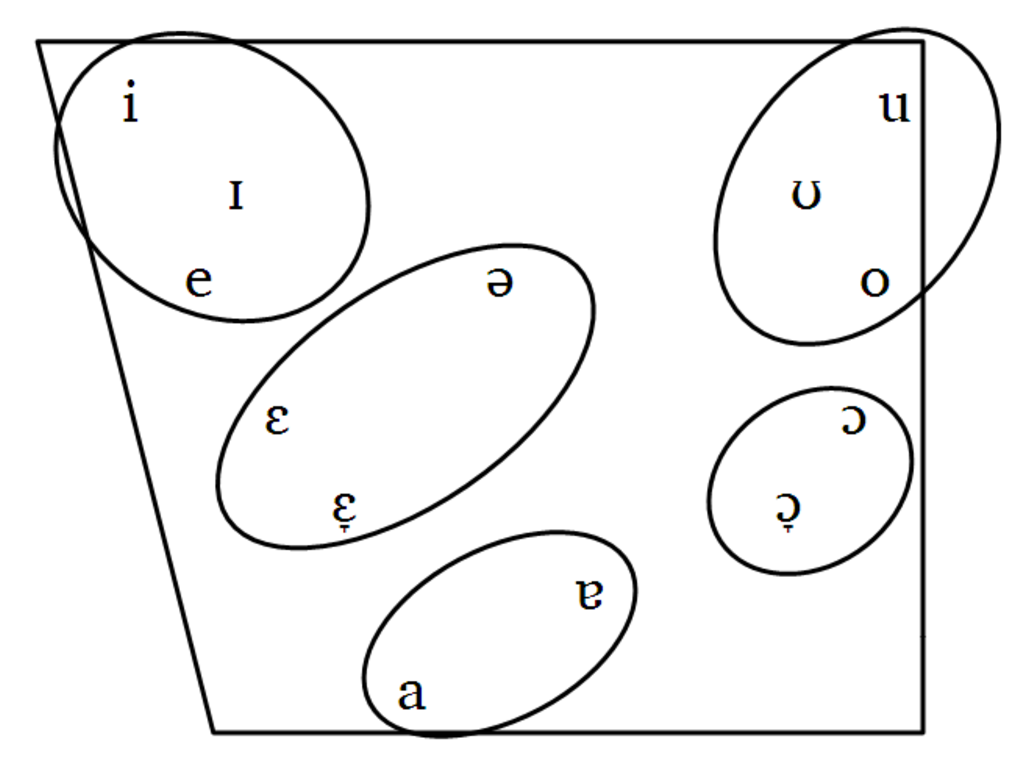
\includegraphics[scale=0.5]{./figures/Figure_2_1}
%\documentclass{article}
%
%\usepackage{tikz}
%\usetikzlibrary{calc}
%\usetikzlibrary{positioning}
%\usetikzlibrary{fit}
%
%\begin{document}

\begin{tikzpicture}[baseline, on grid=true]
\node at (0,0) (ol) {};
\node [right=6cm of ol] (or) {};
\node [below right=4.5cm and 1cm of ol] (ul) {};
\node [below=4.5cm of or] (ur) {};

\draw (ol.center) -- (or.center) -- (ur.center) -- (ul.center) -- (ol.center);

\node[below right=\baselineskip and 0.6cm of ol] (i) {i};
\node[below left=\baselineskip and .25cm of or](u) {u};
\node[below left=\baselineskip and .5cm of u](U) {ʊ};
\node[below right=\baselineskip and .75cm of i] (I) {ɪ};
\node[below right=2\baselineskip and .5cm of i](e) {e};
\node[right=2.25cm of e](E) {ə};
\node[right=2.25cm of E.west](o) {o};
\node[below right=2\baselineskip and .5cm of e](eps) {ε};
\node[right=4cm of eps](oo) {ɔ};
\node[below left=\baselineskip and .5cm of oo](ool) {\textlowering{ɔ}};
\node[below right=\baselineskip and .5cm of eps](epsl) {\textlowering{ε}};

\node[above right=.5\baselineskip and 1.5cm of ul](a) {a};
\node[above right=\baselineskip and 1.25cm of a](A) {ɐ};

\node[draw=black, inner sep=0pt, thick, ellipse, rotate fit=135, fit=(i) (I) (e)] {};
\node[draw=black, inner sep=0pt, thick, ellipse, fit=(u) (U) (o)] {};
\node[draw=black, inner sep=0pt, thick, ellipse, rotate fit=120, fit=(E) (eps) (epsl)] {};
\node[draw=black, inner sep=0pt, thick, ellipse, fit=(a) (A)] {};
\node[draw=black, inner sep=0pt, thick, ellipse, fit=(oo) (ool)] {};


\end{tikzpicture}	
%
%\end{document}
\caption{Vowel space for the Papuan Malay vowels\label{Figure_2.1}}
\end{figure}
 



The phonological processes involved in the allophonic \isi{variation} of the Papuan Malay vowels are discussed in §\ref{Para_2.2.3}.


\subsubsection[Contrast between the vowel segments]{Contrast between the vowel segments\label{Para_2.1.2.2}}

Contrast between the five vowel segments in disyllabic lexical items is presented in minimal or near-minimal pairs in the following tables: in open stressed penultimate syllables in \tabref{Table_2.7}, in closed stressed penultimate syllables in \tabref{Table_2.8}, and in open unstressed ultimate syllables in \tabref{Table_2.9}. When minimal or near-minimal pairs could not be found, another word containing a contrasting vowel segment is given.

\begin{table}
\caption{Vowel contrast in open stressed penultimate syllables\label{Table_2.7}}

\begin{tabular}{llll}

\lsptoprule
 Contrast & Item & Orthogr. & Gloss\\

\midrule
\textstyleChCharisSIL{i{\Tilde}ɛ} & [\textstyleChCharisSIL{ˈi.kʊt̚}] & \textitbf{ikut} & ‘follow’\\
& [\textstyleChCharisSIL{ˈɛ.kɔ̞r}] & \textitbf{ekor} & ‘tail’\\
\textstyleChCharisSIL{i{\Tilde}a} & [\textstyleChCharisSIL{ˈi.ŋɪŋ}] & \textitbf{inging} & ‘wish’\\
& [\textstyleChCharisSIL{ˈa.ŋɪŋ}] & \textitbf{anging} & ‘wind’\\
\textstyleChCharisSIL{i{\Tilde}u} & [\textstyleChCharisSIL{ˈɪ.ɾɪs}] & \textitbf{iris} & ‘cut’\\
& [\textstyleChCharisSIL{ˈʊ.ɾʊs}] & \textitbf{urus} & ‘arrange’\\
\textstyleChCharisSIL{i{\Tilde}ɔ} & [\textstyleChCharisSIL{ˈi.tu}] & \textitbf{itu} & ‘\textsc{d.dist}’\\
& [\textstyleChCharisSIL{ˈɔ.tɔ̞t˺}] & \textitbf{otot} & ‘muscle’\\
\textstyleChCharisSIL{ɛ{\Tilde}a} & [\textstyleChCharisSIL{ˈɛ.dʒɛ̞k̚}] & \textitbf{ejek} & ‘mock’\\
& [\textstyleChCharisSIL{ˈa.dʒɐk}] & \textitbf{ajak} & ‘invite’\\
\textstyleChCharisSIL{ɛ{\Tilde}u} & [\textstyleChCharisSIL{ˈɛ.kɔ̞r}] & \textitbf{ekor} & ‘tail’\\
& [\textstyleChCharisSIL{ˈu.kʊr}] & \textitbf{ukur} & ‘measure’\\
\textstyleChCharisSIL{ɛ{\Tilde}ɔ} & [\textstyleChCharisSIL{ˈɛ.dʒɛ̞k˺}] & \textitbf{ejek} & ‘mock’\\
& [\textstyleChCharisSIL{ˈɔ.dʒɛ̞k˺}] & \textitbf{ojek} & ‘motorbike taxi’\\
\textstyleChCharisSIL{a{\Tilde}u} & [\textstyleChCharisSIL{ˈa.ɾa}] & \textitbf{ara} & ‘direction’\\
& [\textstyleChCharisSIL{ˈu.ɾɐt̚}] & \textitbf{urat} & ‘vein’\\
\textstyleChCharisSIL{u{\Tilde}ɔ} & [\textstyleChCharisSIL{ˈu.dʒʊŋ}] & \textitbf{ujung} & ‘end’\\
& [\textstyleChCharisSIL{ˈɔ.dʒɛ̞k˺}] & \textitbf{ojek} & ‘motorbike taxi’\\
\lspbottomrule
\end{tabular}
\end{table}

\begin{table}
\caption{Vowel contrast in closed stressed penultimate syllables\label{Table_2.8}}

\begin{tabular}{llll}

\lsptoprule
 Contrast & Item & Orthogr. & Gloss\\

\midrule
\textstyleChCharisSIL{i{\Tilde}u} & [\textstyleChCharisSIL{ˈmɪn.ta}] & \textitbf{minta} & ‘request’\\
& [\textstyleChCharisSIL{ˈmʊn.ta}] & \textitbf{munta} & ‘vomit’\\
\textstyleChCharisSIL{i{\Tilde}ɛ} & [\textstyleChCharisSIL{ˈtɪm.bɐŋ}] & \textitbf{timbang} & ‘weigh’\\
& [\textstyleChCharisSIL{ˈtɛ̞m.bɐk̚}] & \textitbf{tembak} & ‘shoot’\\
\textstyleChCharisSIL{i{\Tilde}a} & [\textstyleChCharisSIL{ˈtɪm.ba}] & \textitbf{timba} & ‘fetch’\\
& [\textstyleChCharisSIL{ˈtɐm.ba}] & \textitbf{tamba} & ‘add’\\
\textstyleChCharisSIL{i{\Tilde}ɔ} & [\textstyleChCharisSIL{ˈtɪŋ.kɐt̚}] & \textitbf{tingkat} & ‘level’\\
& [\textstyleChCharisSIL{ˈtɔ̞ŋ.kɐt̚}] & \textitbf{tongkat} & ‘cane’\\
\textstyleChCharisSIL{ɛ{\Tilde}a} & [\textstyleChCharisSIL{ˈsɛ̞n.tu}] & \textitbf{sentu} & ‘touch’\\
& [\textstyleChCharisSIL{ˈsɐn.tɛ}] & \textitbf{sante} & ‘relax’\\
\textstyleChCharisSIL{ɛ{\Tilde}u} & [\textstyleChCharisSIL{ˈtɛ̞m.bɐk̚}] & \textitbf{tembak} & ‘shoot’\\
& [\textstyleChCharisSIL{ˈtʊm.bʊk̚}] & \textitbf{tumbuk} & ‘pound’\\
\textstyleChCharisSIL{ɛ{\Tilde}ɔ} & [\textstyleChCharisSIL{ˈbɛ̞ŋ.kɔ̞k̚}] & \textitbf{bengkok} & ‘be crooked’\\
& [\textstyleChCharisSIL{ˈbɔ̞ŋ.kɔ̞k̚}] & \textitbf{bongkok} & ‘be bent over’\\
\textstyleChCharisSIL{a{\Tilde}u} & [\textstyleChCharisSIL{ˈbɐn.tu}] & \textitbf{bantu} & ‘help’\\
& [\textstyleChCharisSIL{ˈbʊn.tu}] & \textitbf{buntu} & ‘be blocked’\\
\textstyleChCharisSIL{a{\Tilde}ɔ} & [\textstyleChCharisSIL{ˈsɐm.bʊŋ}] & \textitbf{sambung} & ‘continue’\\
& [\textstyleChCharisSIL{ˈsɔ̞m.bɔ̞ŋ}] & \textitbf{sombong} & ‘be arrogant’\\
\textstyleChCharisSIL{u{\Tilde}ɔ} & [\textstyleChCharisSIL{ˈsʊm.bɐŋ}] & \textitbf{sumbang} & ‘donate’\\
& [\textstyleChCharisSIL{ˈsɔ̞m.bɔ̞ŋ}] & \textitbf{sombong} & ‘be arrogant’\\
\lspbottomrule
\end{tabular}
\end{table}

\clearpage

\begin{table}
\caption{Vowel contrast in open unstressed syllables\label{Table_2.9}}

\begin{tabular}{llll}
\lsptoprule
 Contrast & Item & Orthogr. & Gloss\\

\midrule
\textstyleChCharisSIL{i{\Tilde}ɛ} & [\textstyleChCharisSIL{ˈpi.li}] & \textitbf{pili} & ‘choose’\\
& [\textstyleChCharisSIL{ˈpɛ.lɛ}] & \textitbf{pele} & ‘cover’\\
\textstyleChCharisSIL{i{\Tilde}a} & [\textstyleChCharisSIL{ˈka.li}] & \textitbf{kali} & ‘river’\\
& [\textstyleChCharisSIL{ˈka.la}] & \textitbf{kala} & ‘be defeated’\\
\textstyleChCharisSIL{i{\Tilde}u} & [\textstyleChCharisSIL{ˈla.gi}] & \textitbf{lagi} & ‘again’\\
& [\textstyleChCharisSIL{ˈla.gu}] & \textitbf{lagu} & ‘song’\\
\textstyleChCharisSIL{i{\Tilde}ɔ} & [\textstyleChCharisSIL{ˈba.bi}] & \textitbf{babi} & ‘pig’\\
& [\textstyleChCharisSIL{ˈbɔ.bɔ}] & \textitbf{bobo} & ‘palm liquor’\\
\textstyleChCharisSIL{ɛ{\Tilde}u} & [\textstyleChCharisSIL{ˈpa.kɛ}] & \textitbf{pake} & ‘use’\\
& [\textstyleChCharisSIL{ˈpa.ku}] & \textitbf{paku} & ‘nail’\\
\textstyleChCharisSIL{ɛ{\Tilde}ɔ} & [\textstyleChCharisSIL{ˈga.lɛ̞}] & \textitbf{gale} & ‘dig up’\\
& [\textstyleChCharisSIL{ˈga.ɾɔ}] & \textitbf{garo} & ‘scratch’\\
\textstyleChCharisSIL{a{\Tilde}u} & [\textstyleChCharisSIL{ˈbi.sa}] & \textitbf{bisa} & ‘be able’\\
& [\textstyleChCharisSIL{ˈbi.su}] & \textitbf{bisu} & ‘mute’\\
\textstyleChCharisSIL{u{\Tilde}ɔ} & [\textstyleChCharisSIL{ˈtu.bu}] & \textitbf{tubu} & ‘body’\\
& [\textstyleChCharisSIL{ˈtɔ.bɔ}] & \textitbf{tobo} & ‘dive’\\
\lspbottomrule
\end{tabular}
\end{table}

 
\section{Phonological processes\label{Para_2.2}}

In Papuan Malay, two phonological processes are attested for the consonants and one for the vowels: nasal place \isi{assimilation} (§\ref{Para_2.2.1}), tap/trill alternation of the alveolar rhotic (§\ref{Para_2.2.2}), and \isi{centralization} of vowels (§\ref{Para_2.2.3}).


\subsection{Nasal place {assimilation}\label{Para_2.2.1}}
Nasal place \isi{assimilation} applies to nasals as coda in the domain of the prosodic word. While all four nasals occur in the onset position (although velar /\textstyleChCharisSIL{ŋ}/ only occurs in the word-internal onset position), only two nasals occur as coda, namely bilabial /\textstyleChCharisSIL{m}/ and velar /\textstyleChCharisSIL{ŋ}/, as shown in \tabref{Table_2.10}. The velar nasal as a coda assimilates in place of articulation to a following stop or affricate. When preceding the alveolar fricative, the nasal is always realized as velar [\textstyleChCharisSIL{ŋ}], as in \textitbf{bongso} ‘youngest offspring’ or \textitbf{langsung} ‘immediately’. These patterns agree with \citegen[489]{Padgett.1994} cross-linguistic findings that nasals either do “not assimilate in place to fricatives” or that such \isi{assimilation} is, at least, “highly disfavored, while \isi{assimilation} to stops and affricates is pervasive”. (See also \citealt[146--147]{deLacy.2006}; \citealt[554]{Zsiga.2006}; \citealt{Blust.2012}.) An exception to these patterns of nasal \isi{assimilation} is the prefix \textscItal{pe(n)-} ‘\textsc{ag}’ (§\ref{Para_3.1.4}). When preceding the alveolar fricative /s/, the nasal is not realized as alveolar [\textstyleChCharisSIL{n}] but as palatal [\textstyleChCharisSIL{ɲ}], as in \textitbf{penyakit} [\textstyleChCharisSIL{pɛ̞ɲ}–\textstyleChCharisSIL{sakɪt}] ‘disease’, with /\textstyleChCharisSIL{s}/ being deleted (see also \citealt{Blust.2012}; for the \isi{allomorphy} of \textscItal{pe(n)-} see §\ref{Para_3.1.4.1}).


Cross-linguistically, the preservation of the bilabial nasal is not unusual, as \citet[78–207]{deLacy.2006} points out. It is due to the fact, that on the “Place of Articulation” hierarchy, the labial nasal is more marked than the dental or velar ones \citep[129]{deLacy.2006}. Such marked elements “can be specifically targeted for preservation. Consequently, highly marked elements can survive a process that less-marked elements undergo” \citep[146]{deLacy.2006}.\footnote{One anonymous reviewer suggests, however, a different analysis. Given that the nasal in this position obtains its place features from the following segment, not two, but only one nasal phoneme (or ``archiphoneme'') occurs in the word-internal coda position.}

\begin{table}
\caption{Nasal place \isi{assimilation} in the word-internal coda position\label{Table_2.10}}

\begin{tabular}{lllll}
\lsptoprule
 Phoneme & Realization & Item & Orthogr. &  Gloss\\

\midrule
/\textstyleChCharisSIL{m}/ & [\textstyleChCharisSIL{m}] & [\textstyleChCharisSIL{ˈsɪ}\textstyleChCharisSILBlueBold{m}\textstyleChCharisSIL{.}\textstyleChCharisSILBlueBold{p}\textstyleChCharisSIL{ɐŋ}] & \textitbf{simpang} & ‘store’\\
&  & [\textstyleChCharisSIL{kɛ̞}\textstyleChCharisSILBlueBold{m}\textstyleChCharisSIL{.ˈ}\textstyleChCharisSILBlueBold{b}\textstyleChCharisSIL{a.li}] & \textitbf{kembali} & ‘return’\\
/\textstyleChCharisSIL{ŋ}/ & [n] & [\textstyleChCharisSIL{ˈmɪ}\textstyleChCharisSILBlueBold{n}\textstyleChCharisSIL{.}\textstyleChCharisSILBlueBold{t}\textstyleChCharisSIL{a}] & \textitbf{minta} & ‘ask’\\
&  & [\textstyleChCharisSIL{ˈmɐ}\textstyleChCharisSILBlueBold{n}\textstyleChCharisSIL{.}\textstyleChCharisSILBlueBold{d}\textstyleChCharisSIL{i}] & \textitbf{mandi} & ‘bathe’\\
&  & [\textstyleChCharisSIL{ˈhɐ}\textstyleChCharisSILBlueBold{n}\textstyleChCharisSIL{.}\textstyleChCharisSILBlueBold{ʧ}\textstyleChCharisSIL{ʊr}] & \textitbf{hancur} & ‘be shattered’\\
&  & [\textstyleChCharisSIL{ˈɪ}\textstyleChCharisSILBlueBold{n}\textstyleChCharisSIL{.}\textstyleChCharisSILBlueBold{dʒ}\textstyleChCharisSIL{ɐk̚}] & \textitbf{injak} & ‘step on’\\
& [\textstyleChCharisSIL{ŋ}] & [\textstyleChCharisSIL{ˈɐ}\textstyleChCharisSILBlueBold{ŋ}\textstyleChCharisSIL{.}\textstyleChCharisSILBlueBold{k}\textstyleChCharisSIL{ɐt̚}] & \textitbf{angkat} & ‘lift’\\
&  & [\textstyleChCharisSIL{ˈtɪ}\textstyleChCharisSILBlueBold{ŋ}\textstyleChCharisSIL{.}\textstyleChCharisSILBlueBold{g}\textstyleChCharisSIL{i}] & \textitbf{tinggi} & ‘be tall’\\
&  & [\textstyleChCharisSIL{ˈbɔ̞}\textstyleChCharisSILBlueBold{ŋ}\textstyleChCharisSIL{.}\textstyleChCharisSILBlueBold{s}\textstyleChCharisSIL{ɔ̞}] & \textitbf{bongso} & ‘youngest offspring’\\
&  & [\textstyleChCharisSIL{ˈlɐ}\textstyleChCharisSILBlueBold{ŋ}\textstyleChCharisSIL{.}\textstyleChCharisSILBlueBold{s}\textstyleChCharisSIL{ʊŋ}] & \textitbf{langsung} & ‘immediately’\\
\lspbottomrule
\end{tabular}
\end{table}

\largerpage
Nasal place \isi{assimilation} also occurs across word boundaries, when the nasal is in the word-final coda position, as shown in \tabref{Table_2.11}. While bilabial /\textstyleChCharisSIL{m}/ is preserved, velar /\textstyleChCharisSIL{ŋ}/ assimilates in place of articulation to a following stop or affricate, similar to the processes illustrated in \tabref{Table_2.10}. When preceding a fricative-initial or vowel-initial word, or when occurring before a pause or at the end of an utterance, by contrast, the velar nasal is most commonly realized as velar [\textstyleChCharisSIL{ŋ}]. In \tabref{Table_2.11}, this is illustrated with \textitbf{minum} ‘drink’, \textitbf{biking} ‘make’ and \textitbf{bilang} ‘say’. Overall, however, \isi{assimilation} across word boundaries is applied less often than within the prosodic word.

\begin{table}
\caption{Nasal place \isi{assimilation} in the word-final coda position\label{Table_2.11}}

\begin{tabular}{llll}
\lsptoprule
 Phoneme & Item & Orthogr. &  Gloss\\
\midrule
/\textstyleChCharisSIL{m}/ & [\textstyleChCharisSIL{ˈmi.nʊ}\textstyleChCharisSILBlueBold{m}\textstyleChCharisSIL{ ˈ}\textstyleChCharisSILBlueBold{b}\textstyleChCharisSIL{ɔ.bɔ}] & \textitbf{minum bobo} & ‘drink schnapps’\\
& [\textstyleChCharisSIL{ˈmi.nʊ}\textstyleChCharisSILBlueBold{m}\textstyleChCharisSIL{ ˈ}\textstyleChCharisSILBlueBold{d}\textstyleChCharisSIL{u.lu}] & \textitbf{minum dulu} & ‘drink first’\\
& [{\ldots} \textstyleChCharisSIL{ˈmi.nʊ}\textstyleChCharisSILBlueBold{m}\textstyleChCharisSIL{ ˈ}\textstyleChCharisSILBlueBold{k}\textstyleChCharisSIL{i.ˈtɔ̞ŋ}] & \textitbf{{\ldots} minum kitong} & ‘(give) us to drink’\\
& [\textstyleChCharisSIL{ˈmi.nʊ}\textstyleChCharisSILBlueBold{m}\textstyleChCharisSIL{ ˈ}\textstyleChCharisSILBlueBold{i}\textstyleChCharisSIL{.tu}] & \textitbf{minum itu} & ‘drink that’\\
& [\textstyleChCharisSIL{ˈmi.nʊ}\textstyleChCharisSILBlueBold{m}\textstyleChCharisSIL{, ˈ}\textstyleChCharisSILBlueBold{t}\textstyleChCharisSIL{a.pi}] & \textitbf{minum, tapi} & ‘drink, but’\\
/\textstyleChCharisSIL{ŋ}/ & [\textstyleChCharisSIL{ˈbi.kɪ}\textstyleChCharisSILBlueBold{m}\textstyleChCharisSIL{ ˈ}\textstyleChCharisSILBlueBold{b}\textstyleChCharisSIL{a.gʊs}] & \textitbf{biking bagus} & ‘make good’\\
& [\textstyleChCharisSIL{ˈbi.kɪ}\textstyleChCharisSILBlueBold{n}\textstyleChCharisSIL{ ˈ}\textstyleChCharisSILBlueBold{d}\textstyleChCharisSIL{ɪ.a}] & \textitbf{biking dia} & ‘make him/her’\\
& [\textstyleChCharisSIL{ˈbi.kɪ}\textstyleChCharisSILBlueBold{ŋ}\textstyleChCharisSIL{ ˈ}\textstyleChCharisSILBlueBold{k}\textstyleChCharisSIL{ɔ.tɔ̞r}] & \textitbf{biking kotor} & ‘make dirty’\\
& [\textstyleChCharisSIL{ˈbi.kɪ}\textstyleChCharisSILBlueBold{ŋ}\textstyleChCharisSIL{ ˈ}\textstyleChCharisSILBlueBold{s}a] & \textitbf{biking sa} & ‘make me’\\
& [\textstyleChCharisSIL{ˈbi.kɪ}\textstyleChCharisSILBlueBold{ŋ}\textstyleChCharisSIL{ ˈ}\textstyleChCharisSILBlueBold{a}\textstyleChCharisSIL{.pa}] & \textitbf{biking apa} & ‘make what’\\
& [\textstyleChCharisSIL{ˈbi.kɪ}\textstyleChCharisSILBlueBold{ŋ}\textstyleChCharisSIL{, ˈ}\textstyleChCharisSILBlueBold{m}\textstyleChCharisSIL{ɛ.mɐŋ}] & \textitbf{biking, memang} & ‘make, indeed’\\
/\textstyleChCharisSIL{ŋ}/ & [\textstyleChCharisSIL{ˈbi.lɐ}\textstyleChCharisSILBlueBold{m}\textstyleChCharisSIL{ ˈ}\textstyleChCharisSILBlueBold{b}\textstyleChCharisSIL{a.pa}] & \textitbf{bilang bapa} & ‘tell father’\\
& [\textstyleChCharisSIL{ˈbi.lɐ}\textstyleChCharisSILBlueBold{n}\textstyleChCharisSIL{ ˈ}\textstyleChCharisSILBlueBold{d}\textstyleChCharisSIL{ɪ.a}] & \textitbf{bilang dia} & ‘tell him/her’\\
& [\textstyleChCharisSIL{ˈbi.lɐ}\textstyleChCharisSILBlueBold{ŋ}\textstyleChCharisSIL{ ˈ}\textstyleChCharisSILBlueBold{k}\textstyleChCharisSIL{a.ka}] & \textitbf{bilang kaka} & ‘tell older sibling’\\
& [\textstyleChCharisSIL{ˈbi.lɐ}\textstyleChCharisSILBlueBold{ŋ}\textstyleChCharisSIL{ ˈ}\textstyleChCharisSILBlueBold{s}a\textstyleChCharisSIL{.ma}] & \textitbf{bilang sama} & ‘say to’\\
& [\textstyleChCharisSIL{ˈbi.lɐ}\textstyleChCharisSILBlueBold{ŋ}\textstyleChCharisSIL{ ˈ}\textstyleChCharisSILBlueBold{i}\textstyleChCharisSIL{.ni}] & \textitbf{bilang ini} & ‘say this’\\
& [\textstyleChCharisSIL{ˈbi.lɐ}\textstyleChCharisSILBlueBold{ŋ}\textstyleChCharisSIL{, ˈ}\textstyleChCharisSILBlueBold{b}\textstyleChCharisSIL{lʊm}] & \textitbf{bilang, blum} & ‘say, not yet’\\
\lspbottomrule
\end{tabular}
\end{table}

In summary, the data presented in \tabref{Table_2.10} and \tabref{Table_2.11} shows that Papuan Malay has only two underlying nasals in the coda position, namely bilabial /\textstyleChCharisSIL{m}/ and velar /\textstyleChCharisSIL{ŋ}/, with the latter assimilating to a following stop or affricate.

\newpage 

\subsection{Tap/trill alternation of the alveolar rhotic\label{Para_2.2.2}}
The rhotic /r/ is most commonly realized as the voiced alveolar trill [\textstyleChCharisSIL{r}]. In inter-vocalic position, however, the rhotic is realized as the voiced tap [\textstyleChCharisSIL{ɾ}] as illustrated in (\ref{Example_2.1}) and \tabref{Table_2.12}.\footnote{In the examples in this chapter, the first line gives the orthographic representation, while the second lines gives the IPA transcription.} In the C\textsubscript{2} position in CC clusters, the rhotic is also most commonly realized as the voiced trill [r]. The voiced tap, however, is also quite common in this position.

\ea
\label{Example_2.1}
\gll {ta}  { pake}  {\ldots}  {ga\bluebold{ɾ}ɐɐɐm}  {s\bluebold{r}ej}  {\bluebold{r}iʧaaa}  {\ldots}  {dagɪŋ}  {ini}\\
\textsc{1pl}  {take} { }  {salt} {lemongrass}  {red.pepper} {}    {meat}  \textsc{d.prox}\\
\gll {saja}  {asa\bluebold{r}}  dia  {kasi}  {k\bluebold{r}ing}  {di }  {pa\bluebold{r}apa\bluebold{r}a}\\
{\textsc{1sg}}  {smoke}  \textsc{3sg}  {give}  be.dry  {at}  {platform}\\
\glt ‘we used {\ldots} \bluebold{salt}, \bluebold{lemongrass}, \bluebold{red pepper}, {\ldots} this (pig) meat, I \bluebold{smoked} it (and) \bluebold{dried} (it) on a \bluebold{platform}’ \textstyleExampleSource{[080919-004-NP.0037-0038]} \\
\z


\begin{table}
\caption{Tap/trill alternation of rhotic /\textstyleChCharisSIL{r}/\label{Table_2.12}}

\begin{tabular}{llll}
\lsptoprule
 Realization & Item & Orthogr. &  Gloss\\

\midrule

[\textstyleChCharisSIL{r}] & [\textstyleChCharisSIL{ˈ}\textstyleChCharisSILBlueBold{r}\textstyleChCharisSIL{a.kʊs}] & \textitbf{rakus} & ‘be greedy’\\
 & [\textstyleChCharisSIL{ˈk}\textstyleChCharisSILBlueBold{r}\textstyleChCharisSIL{i.ŋɐt̚}] & \textitbf{kringat} & ‘sweat’\\
 & [\textstyleChCharisSIL{ˈmʊ}\textstyleChCharisSILBlueBold{r}\textstyleChCharisSIL{.ni}] & \textitbf{murni} & ‘be pure’\\
 & [\textstyleChCharisSIL{ˈdʒɐŋ.k}\textstyleChCharisSILBlueBold{r}\textstyleChCharisSIL{ɪk̚}] & \textitbf{jangkrik} & ‘cricket’\\
 
[\textstyleChCharisSIL{ɾ}] & [\textstyleChCharisSIL{ˈba.}\textstyleChCharisSILBlueBold{ɾ}\textstyleChCharisSIL{ɐŋ}] & \textitbf{barang} & ‘stuff’\\
 & [\textstyleChCharisSIL{ˈgɔ.}\textstyleChCharisSILBlueBold{ɾ}\textstyleChCharisSIL{ɛ̞ŋ}] & \textitbf{goreng} & ‘fry’\\
 & [\textstyleChCharisSIL{ˈʊ.}\textstyleChCharisSILBlueBold{ɾ}\textstyleChCharisSIL{ʊs}] & \textitbf{urus} & ‘arrange’\\

\lspbottomrule

\end{tabular}
\end{table}

\newpage 
\subsection{Centralization of vowels\label{Para_2.2.3}}
In closed syllables the five vowels are centralized. Close /\textstyleChCharisSIL{i}/ is centralized to [\textstyleChCharisSIL{ɪ}] and /\textstyleChCharisSIL{u}/ to [\textstyleChCharisSIL{ʊ}], open-mid /\textstyleChCharisSIL{ɛ}/ is centralized to [\textstyleChCharisSIL{ɛ̞}] and /\textstyleChCharisSIL{ɔ}/ to [\textstyleChCharisSIL{ɔ̞}], and open /\textstyleChCharisSIL{a}/ is centralized to [\textstyleChCharisSIL{ɐ}], as illustrated in \tabref{Table_2.13}. In unstressed closed syllables with a coda nasal, open-mid /\textstyleChCharisSIL{ɛ}/ can alternatively be centralized to [\textstyleChCharisSIL{ə}] rather than to [\textstyleChCharisSIL{ɛ̞}].

\begin{table}
\caption{Vowel \isi{centralization} in closed syllables\label{Table_2.13}}

\begin{tabular}{cclll}
\lsptoprule
 Phoneme & Realization & \multicolumn{1}{c}{Item} &  \multicolumn{1}{c}{Orthogr.} &   \multicolumn{1}{c}{Gloss}\\


\midrule
/\textstyleChCharisSIL{i}/ & [\textstyleChCharisSIL{ɪ}] & [\textstyleChCharisSIL{ˈt}\textstyleChCharisSILBlueBold{ɪ}\textstyleChCharisSIL{ŋ.gi}] & \textitbf{tinggi} & ‘be high’\\
&  & [\textstyleChCharisSIL{ˈa.d}\textstyleChCharisSILBlueBold{ɪ}\textstyleChCharisSIL{l}] & \textitbf{adil} & ‘be fair’\\
/\textstyleChCharisSIL{u}/ & [\textstyleChCharisSIL{ʊ}] & [\textstyleChCharisSIL{ˈb}\textstyleChCharisSILBlueBold{ʊ}\textstyleChCharisSIL{ŋ.k}\textstyleChCharisSILBlueBold{ʊ}\textstyleChCharisSIL{s}] & \textitbf{bungkus} & ‘pack’\\
&  & [\textstyleChCharisSIL{ˈi.k}\textstyleChCharisSILBlueBold{ʊ}\textstyleChCharisSIL{t̚}] & \textitbf{ikut} & ‘follow’\\
/\textstyleChCharisSIL{ɛ}/ & [\textstyleChCharisSIL{ɛ̞}] & [\textstyleChCharisSIL{ˈg}\textstyleChCharisSILBlueBold{ɛ̞}\textstyleChCharisSIL{n.dɔ̞ŋ}] & \textitbf{gendong} & ‘hold’\\
&  & [\textstyleChCharisSIL{ˈdɔ.ŋ}\textstyleChCharisSILBlueBold{ɛ̞}\textstyleChCharisSIL{ŋ}] & \textitbf{dongeng} & ‘legend’\\
& [\textstyleChCharisSIL{ə}] & [\textstyleChCharisSILBlueBold{ə}\textstyleChCharisSIL{m.ˈpɐt̚}] & \textitbf{empat} & ‘four’\\
&  & [\textstyleChCharisSIL{s}\textstyleChCharisSILBlueBold{ə}\textstyleChCharisSIL{m.ˈbi.lɐŋ}] & \textitbf{sembilang} & ‘nine’\\
/\textstyleChCharisSIL{ɔ}/ & [\textstyleChCharisSIL{ɔ̞}] & [\textstyleChCharisSIL{ˈl}\textstyleChCharisSILBlueBold{ɔ̞}\textstyleChCharisSIL{m.ba}] & \textitbf{lomba} & ‘contest’\\
&  & [\textstyleChCharisSIL{ˈbɛ.l}\textstyleChCharisSILBlueBold{ɔ̞}\textstyleChCharisSIL{k̚}] & \textitbf{belok} & ‘turn’\\
/\textstyleChCharisSIL{a}/ & [\textstyleChCharisSIL{ɐ}] & [\textstyleChCharisSIL{ˈ}\textstyleChCharisSILBlueBold{ɐ}\textstyleChCharisSIL{n.dʒɪŋ}] & \textitbf{anjing} & ‘dog’\\
&  & [\textstyleChCharisSIL{ˈbɪn.t}\textstyleChCharisSILBlueBold{ɐ}\textstyleChCharisSIL{ŋ}] & \textitbf{bintang} & ‘star’\\
\lspbottomrule
\end{tabular}
\end{table}
\section{Phonetic processes\label{Para_2.3}}

In Papuan Malay, a number of phonetic processes occur in addition to the predictable phonological processes described in §\ref{Para_2.2}. These surface phenomena involve unpredict\-able \isi{variation}. For the consonants, the following phenomena are attested: \isi{lenition} of the stops and the voiced affricates as well as \isi{fortition} of the voiceless affricate and the palatal approximant (§\ref{Para_2.3.1.1}), \isi{elision} of the voiceless stops, the alveolar fricative, the velar nasal, and the liquids (§\ref{Para_2.3.1.2}), and \isi{devoicing} of the alveolar rhotic (§\ref{Para_2.3.1.3}). The vowels can undergo the following phonetic processes: \isi{centralization} and \isi{lowering} (§\ref{Para_2.3.2.1}), \isi{nasalization} (§\ref{Para_2.3.2.2}), and \isi{lengthening} (§\ref{Para_2.3.2.3}). In addition, this section includes a discussion on alternative realizations of the VC sequences /\textstyleChCharisSIL{aj}/ and /\textstyleChCharisSIL{aw}/ (§\ref{Para_2.3.3})


\subsection{Phonetic processes for consonants\label{Para_2.3.1}}
\subsubsection[Lenition and {fortition}]{Lenition and {fortition}\label{Para_2.3.1.1}}
 
Lenition, or weakening, is attested for the stops and affricates and can occur in word-internal inter-vocalic position, and word-initial position. Fortition, or strengthening, occurs very rarely and is only attested for the voiceless affricate and the palatal approximant as word-initial onset.


Most of the stops and the voiced affricate can also be lenited in word-initial position when following a word with final vowel. In this environment, however, \isi{lenition} of the voiced affricate occurs less often than \isi{lenition} of the stops. Inter-vocalically across word-boundaries, the word-initial obstruents are lenited to the same fricatives as word-internally, as shown in \tabref{Table_2.15}. Also, /\textstyleChCharisSIL{p}/ can be lenited to [\textstyleChCharisSIL{f}], and /\textstyleChCharisSIL{d}/ and /\textstyleChCharisSIL{d}\textstyleChCharisSIL{ʒ}/ can be lenited to [\textstyleChCharisSIL{j}]. Word-initial \isi{lenition} to a fricative is also attested for /\textstyleChCharisSIL{b}/, /\textstyleChCharisSIL{d}/, and /\textstyleChCharisSIL{k}/ when following a nasal. In this environment, /\textstyleChCharisSIL{d}/ can also be lenited to [\textstyleChCharisSIL{n}]. Again, \isi{lenition} to a fricative is unattested for the voiceless alveolar and palato-alveolar segments. Likewise, \isi{lenition} in word-initial position is unattested for /\textstyleChCharisSIL{g}/.\footnote{One lexical item in particular undergoes \isi{lenition} of its word-initial stop: the long and the short forms of the third person singular \isi{pronoun}, \textitbf{dia}/\textitbf{de} ‘\textsc{3sg}’. Onset /\textstyleChCharisSILviiivpt{d}/ can be lenited to [\textstyleChCharisSILviiivpt{j}] when following a lexical item with a voiceless stop, the alveolar fricative /\textstyleChCharisSILviiivpt{s}/, or the rhotic /\textstyleChCharisSILviiivpt{r}/ in word-final coda position.}



\begin{table} 
\caption{Lenition of stops and affricates in word-internal inter-vocalic position\label{Table_2.14}}

\begin{tabular}{clll}
\lsptoprule
 Phoneme &  \multicolumn{1}{c}{Item} &  \multicolumn{1}{c}{Orthogr.} &   \multicolumn{1}{c}{Gloss}\\

\midrule
/\textstyleChCharisSIL{p}/ & [\textstyleChCharisSIL{ˈba.}\textstyleChCharisSILBlueBold{ɸ}\textstyleChCharisSIL{a}] & \textitbf{bapa} & ‘father’\\
/\textstyleChCharisSIL{b}/ & [\textstyleChCharisSIL{ˈsa.}\textstyleChCharisSILBlueBold{β}\textstyleChCharisSIL{ɐr}] & \textitbf{sabar} & ‘be patient’\\
/\textstyleChCharisSIL{d}/ & [\textstyleChCharisSIL{ˈsʊ.}\textstyleChCharisSILBlueBold{ð}\textstyleChCharisSIL{a}] & \textitbf{suda} & ‘already’\\
/\textstyleChCharisSIL{k}/ & [\textstyleChCharisSIL{ˈma.}\textstyleChCharisSILBlueBold{x}\textstyleChCharisSIL{ɐŋ}] & \textitbf{makang} & ‘eat’\\
/\textstyleChCharisSIL{g}/ & [\textstyleChCharisSIL{ˈba.}\textstyleChCharisSILBlueBold{ɣ}\textstyleChCharisSIL{i}] & \textitbf{bagi} & ‘divide’\\
/\textstyleChCharisSIL{d}\textstyleChCharisSIL{ʒ}/ & [\textstyleChCharisSIL{ˈsa.}\textstyleChCharisSILBlueBold{ʝ}\textstyleChCharisSIL{a}] & \textitbf{saja} & ‘just’\\
/\textstyleChCharisSIL{t}\textstyleChCharisSIL{ʃ}/ & [\textstyleChCharisSIL{ˈpa.}\textstyleChCharisSILBlueBold{j}\textstyleChCharisSIL{ɛ}] & \textitbf{pace} & ‘man’\\
\lspbottomrule
\end{tabular}
\end{table}



Inter-vocalically, the stops and the voiced affricate can be lenited by means of spirantization to fricatives, as illustrated in \tabref{Table_2.14}: /\textstyleChCharisSIL{p}/ is lenited to [\textstyleChCharisSIL{ɸ}], /\textstyleChCharisSIL{b}/ to [\textstyleChCharisSIL{β}], /\textstyleChCharisSIL{d}/ to [\textstyleChCharisSIL{ð}], /\textstyleChCharisSIL{k}/ to [\textstyleChCharisSIL{x}], /\textstyleChCharisSIL{g}/ to [\textstyleChCharisSIL{ɣ}], and /\textstyleChCharisSIL{d}\textstyleChCharisSIL{ʒ}/ to [\textstyleChCharisSIL{ʝ}]. This process is unattested, however, for the voiceless alveolar and palato-alveolar segments. The voiceless affricate /\textstyleChCharisSIL{t}\textstyleChCharisSIL{ʃ}/ can be lenited to the palatal approximant [\textstyleChCharisSIL{j}], while \isi{lenition} of alveolar /\textstyleChCharisSIL{t}/ is unattested.




\begin{table}[t] 
\caption{Lenition of stops and affricates in word-initial position\label{Table_2.15}}


\begin{tabular}{clll}
\lsptoprule
 Phoneme &  \multicolumn{1}{c}{Item} &  \multicolumn{1}{c}{Orthogr.} &   \multicolumn{1}{c}{Gloss}\\

\midrule
/\textstyleChCharisSIL{p}/ & [\textstyleChCharisSIL{ˈdɛ }\textstyleChCharisSILBlueBold{ɸ}\textstyleChCharisSIL{u}] & \textitbf{de pu} & ‘his (grandson)’\\
&  & \textsc{3sg} \textsc{poss} & \\
& [\textstyleChCharisSIL{ˈdi.a ˈ}\textstyleChCharisSILBlueBold{f}\textstyleChCharisSIL{luŋ.ku}] & \textitbf{dia palungku} & ‘he punched’\\
&  & \textsc{3sg} punch & \\

/\textstyleChCharisSIL{b}/ & [\textstyleChCharisSIL{ˈjɛ ˈ}\textstyleChCharisSILBlueBold{β}\textstyleChCharisSIL{i.lɐŋ}] & \textitbf{de bilang} & ‘he/she said’\\
&  & \textsc{3sg} say & \\
& [\textstyleChCharisSIL{ˈdʒa.rɪm ˈ}\textstyleChCharisSILBlueBold{β}\textstyleChCharisSIL{ɔ.lɛ}] & \textitbf{jaring bole} & (the) net (is) permitted\\
&  & net may & \\

/\textstyleChCharisSIL{d}/ & [\textstyleChCharisSIL{mˈla, ɛ ˈ}\textstyleChCharisSILBlueBold{ð}\textstyleChCharisSIL{ɛ̞p̚}] & \textitbf{mulay, eh dep} & ‘(he) started, uh his’\\
&  & start uh \textsc{3sg:poss} & \\
& [\textstyleChCharisSIL{ˈsa.dʒa }\textstyleChCharisSILBlueBold{j}\textstyleChCharisSIL{ɛ̞.ˈŋɐŋ}] & \textitbf{saja dengang} & ‘just with’\\
&  & just with & \\
& [\textstyleChCharisSIL{ˈspʊl ˈba.ðɐn ˈ}\textstyleChCharisSILBlueBold{ð}\textstyleChCharisSIL{i}] & \textitbf{spul badang di} & ‘wash (your) body in’\\
&  & wash body at & \\
& [\textstyleChCharisSIL{ˈki.tɔ̞n ˈ}\textstyleChCharisSILBlueBold{n}\textstyleChCharisSIL{u.a}] & \textitbf{kitong dua} & ‘we two’\\
&  & \textsc{1pl} two & \\

/\textstyleChCharisSIL{k}/ & [\textstyleChCharisSIL{ˈa.dɛ̞.ˈ}\textstyleChCharisSILBlueBold{x}\textstyleChCharisSIL{a.xa}] & \textitbf{ade-kaka} & ‘siblings’\\
&  & ySb oSb & \\
& [\textstyleChCharisSIL{dɛ̞.ˈŋɐŋ ˈ}\textstyleChCharisSILBlueBold{x}\textstyleChCharisSIL{a.xa}] & \textitbf{dengang kaka} & ‘with (the) older sibling’\\
&  & with oSb & \\

/\textstyleChCharisSIL{d}\textstyleChCharisSIL{ʒ}/ & [\textstyleChCharisSIL{ˈsa pu ˈ}\textstyleChCharisSILBlueBold{ʝ}\textstyleChCharisSIL{ɛ̞.kɛ̞t˺}] & \textitbf{sa pu jeket} & ‘my jacket’\\
&  & 1\textsc{sg} \textsc{poss} jacket & \\
& [\textstyleChCharisSIL{{\ldots} ˈi.tu, ˈ}\textstyleChCharisSILBlueBold{j}\textstyleChCharisSIL{a.ŋɐŋ}] & \textitbf{{\ldots} itu, jangang} & ‘those (big ones), don’t’\\
&  & \textsc{d.dist} \textsc{neg.imp} & \\
\lspbottomrule
\end{tabular}
\end{table}





  
Fortition occurs very rarely and is attested only for the voiceless affricate and the palatal approximant in word-initial position. In the more thoroughly transcribed 150-minute extract of the corpus, \isi{fortition} of /\textstyleChCharisSIL{t}\textstyleChCharisSIL{ʃ}/ is attested once and strengthening of /\textstyleChCharisSIL{j}/ twice, as shown in \tabref{Table_2.16}.

\begin{table}[p]
\caption{ Fortition of the voiceless affricate and the voiced palatal approximant\label{Table_2.16}}
\begin{tabular}{clll}
\lsptoprule
Phoneme &  \multicolumn{1}{c}{Item} &  \multicolumn{1}{c}{Orthogr.} &   \multicolumn{1}{c}{Gloss}\\
\midrule
/\textstyleChCharisSIL{ʧ}/ & [\textstyleChCharisSIL{ˈdɛ̞p˺} \textstyleChCharisSILBlueBold{ˈt}\textstyleChCharisSIL{u.ʧu}] & \textitbf{de pu cucu} & ‘his grandchild’\\
&  & \textsc{3sg} \textsc{poss} grandchild & \\

/\textstyleChCharisSIL{j} / & [\textstyleChCharisSIL{ˈej} \textstyleChCharisSILBlueBold{ˈdʒ}\textstyleChCharisSIL{ɐŋ bɛ.}ˌ\textstyleChCharisSIL{sɐr{\Tilde}bɛ.ˈsɐr}] & \textitbf{ey yang {besar{\Tilde}besar}} & ‘hey those big ones’\\
&  & hey \textsc{rel} \textsc{rdp} {\Tilde}be.big & \\
& [\textstyleChCharisSIL{ˈ}\textstyleChCharisSILBlueBold{ʝ}\textstyleChCharisSIL{a}] & \textitbf{yo} & ‘yes’\footnote{Affirmative \textitbf{yo} ‘yes’ is frequently realized as \textitbf{ya} (see §\ref{Para_5.4.3}).}\\
&  & yes & \\
\lspbottomrule
\end{tabular}
\end{table}



\subsubsection[Elision]{Elision\label{Para_2.3.1.2}}
 
Elision of a word-final segment is attested for the voiceless stops, the alveolar fricative, the velar nasal, and both liquids, as shown in \tabref{Table_2.17}. Concerning the voiceless stops, \isi{elision} applies most frequently to /\textstyleChCharisSIL{k}/. Elision of /\textstyleChCharisSIL{t}/ occurs less frequently and is unattested for /\textstyleChCharisSIL{p}/. Word-final /\textstyleChCharisSIL{s}/ is much less prone to \isi{elision} than word-final stops, with the corpus containing only two lexical items with deleted /\textstyleChCharisSIL{s}/. When the word-final velar nasal is omitted, it is always realized as \isi{nasalization} on the preceding vowel.\footnote{More in-depth acoustic phonetic analysis is needed to determine whether the nasalized vowels remain centralized. Since these vowels occur in open syllables they are represented as their non-centralized allophones (for more details see §\ref{Para_2.2.3}) pending further results.} Elision of the liquids occurs only very rarely. The exception is \textitbf{ambil} ‘fetch’. Of its 221 tokens, 49 tokens are realized without word-final /\textstyleChCharisSIL{l}/: [\textstyleChCharisSIL{ˈɐm.bi}] (48 tokens) and [\textstyleChCharisSIL{ˈɐm.be.a}] (1 token).

\begin{table}
\caption[Elision of the voiceless stops\ldots]{Elision of the voiceless stops, the alveolar fricative, the velar nasal, and the liquids in word-final position\label{Table_2.17}}

\begin{tabular}{clll}
\lsptoprule
 Phoneme &  \multicolumn{1}{c}{Item} &  \multicolumn{1}{c}{Orthogr.} &   \multicolumn{1}{c}{Gloss}\\
\midrule

/\textstyleChCharisSIL{t}/ & [\textstyleChCharisSIL{ˈsa.ki}] & \textitbf{sakit} & ‘be sick’\\
/\textstyleChCharisSIL{k}/ & [\textstyleChCharisSIL{ˈma.sa}] & \textitbf{masak} & ‘cook’\\
/\textstyleChCharisSIL{s}/ & [\textstyleChCharisSIL{ˈtru}] & \textitbf{trus} & ‘be continuous’\\
/\textstyleChCharisSIL{ŋ}/ & [\textstyleChCharisSIL{ˈɐn.dʒ\~{i}}] & \textitbf{anjing} & ‘dog’\\
/\textstyleChCharisSIL{r}/ & [\textstyleChCharisSIL{ˈla.pa}] & \textitbf{lapar} & ‘be hungry’\\
/\textstyleChCharisSIL{l}/ & [\textstyleChCharisSIL{ˈɐm.bi} / \textstyleChCharisSIL{ˈɐm.be.a}] & \textitbf{ambil} & ‘fetch’\\

\lspbottomrule
\end{tabular}
\end{table}
\subsubsection[Devoicing]{Devoicing\label{Para_2.3.1.3}}

Devoicing applies only to the rhotic trill as word-final coda. In this position, it is most commonly realized as [\textstyleChCharisSIL{r}]. Before a pause or in utterance-final position, however, the trill can also be devoiced to [\textstyleChCharisSIL{r̥}], as illustrated in (\ref{Example_2.2}).


\ea
\label{Example_2.2}
\gll \bluebold{skaɾɐn}  dɔ̞ŋ  kasi  dɪa  \bluebold{sɛ̞ntɛ̞r̥},  kasi  \bluebold{sɛ̞ntɛ̞r}  dɔ̞ŋ  kasi {\ldots}\\
now  \textsc{3pl}  give  \textsc{3sg}  flashlight  give  flashlight  \textsc{3pl}  give {}\\
\glt
‘\bluebold{now} they give him a \bluebold{flashlight}, (having) given (him) a \bluebold{flashlight} they give (him) \ldots’ \textstyleExampleSource{[081108-003-JR.0002]}\\
\z

\subsubsection[Palatalization]{Palatalization\label{Para_2.3.1.4}}

Palatalization of /\textstyleChCharisSIL{s}/ is rare. It occurs only in lexical roots with a /\textstyleChCharisSIL{si.}V/ sequence, if this root has three or more syllables and if the syllable containing /s/ is unstressed. The \isi{palatalization} of /\textstyleChCharisSIL{s}/ co-occurs with the \isi{elision} of the close front vowel /\textstyleChCharisSIL{i}/, which reduces the number of syllables by one, as illustrated in \tabref{Table_2.18}. Hence, /\textstyleChCharisSIL{si.}V/ is realized as [\textstyleChCharisSIL{sʲ}V]. Attested is one polysyllabic \isi{lexical root} with a /\textstyleChCharisSIL{si.}V/ sequence, the high frequency item \textitbf{siapa} ‘who’. In lexical roots with a /\textstyleChCharisSIL{si.}V/ sequence in which the syllable containing /s/ is stressed, \isi{palatalization} of the fricative is unattested. Attested are the three lexical roots listed in \tabref{Table_2.18}, all of which are disyllabic: \textitbf{sial} ‘be unfortunate’, \textitbf{siang} ‘midday’, and \textitbf{siap} ‘be ready’.


This lack of \isi{assimilation} in stressed syllables does, however, also apply to lexical items with more than two syllables, as evidenced by three polysyllabic loanwords, presented in §\ref{Para_2.5.2.3}. The occurrence of /\textstyleChCharisSIL{s}/ in a /\textstyleChCharisSIL{si.}V/ sequence together with the \isi{stress pattern} of the respective lexical item does not, however, \isi{condition} the \isi{palatalization} of the fricative. This is evidenced by the fact that \textitbf{siapa} ‘who’ is realized quite commonly without \isi{palatalization}: [\textstyleChCharisSIL{ˈsa.pa}].



The frequency counts in \tabref{Table_2.18} are based on the broad transcription of the entire 16-hour corpus (16-\textsc{h-c}) and the more thoroughly transcribed 150-minute extract (150-\textsc{m-c}).\footnote{The broad transcription of the 16-hour corpus makes no distinction between the unpalatalized and the palatalized realizations of \textitbf{siapa} ‘who’, [\textstyleChCharisSILviiivpt{si.ˈa.pa}] and [\textstyleChCharisSILviiivpt{ˈsʲa.pa}], respectively. Hence, a more thorough transcription of all 196 /\textstyleChCharisSILviiivpt{siapa}/ tokens is required to establish whether speakers sometimes realize the \isi{interrogative} as the trisyllabic item [\textstyleChCharisSILviiivpt{si.ˈa.pa}] or whether they always palatalize the fricative and thereby realize the item as disyllabic [\textstyleChCharisSILviiivpt{ˈsʲa.pa}]. In the more thoroughly transcribed 150-minute extract of the corpus the trisyllabic \textitbf{siapa} [\textstyleChCharisSILviiivpt{si.ˈa.pa}] ‘who’ is unattested.}

\begin{table}
\caption{Palatalization of the alveolar fricative in loanwords\label{Table_2.18}}

\begin{tabularx}{\textwidth}{lp{1.2cm}p{2.5cm}Xrr}
\lsptoprule
 \multicolumn{1}{c}{Stress} & \multicolumn{1}{c}{Orthogr.} & \multicolumn{1}{c}{Gloss} & \multicolumn{1}{c}{Realization} & \multicolumn{1}{c}{Freq.} &  \multicolumn{1}{c}{Freq.}\\
&  &  &  & 16-\textsc{h-c} &  150-\textsc{m-c}\\

\midrule
/\textstyleChCharisSIL{si}/ unstressed & \textitbf{siapa} & ‘who’ & [\textstyleChCharisSILBlueBold{si.ˈa}\textstyleChCharisSIL{.pa}] &  196 &  {}-{}-{}-\\
&  &  & [\textstyleChCharisSIL{ˈ}\textstyleChCharisSILBlueBold{sʲa}\textstyleChCharisSIL{.pa}] &  {}-{}-{}- &  40\\
&  &  & [\textstyleChCharisSIL{ˈ}\textstyleChCharisSILBlueBold{sa}\textstyleChCharisSIL{.pa}] &  115 &  10\\
/\textstyleChCharisSIL{ˈsi}/ stressed & \textitbf{sial} & ‘be unfortunate’ & [\textstyleChCharisSIL{ˈ}\textstyleChCharisSILBlueBold{si.ɐ}\textstyleChCharisSIL{l}] &  1 &  1\\
& \textitbf{siang} & ‘midday’ & [\textstyleChCharisSIL{ˈ}\textstyleChCharisSILBlueBold{si.ɐ}\textstyleChCharisSIL{ŋ}] &  55 &  6\\
& \textitbf{siap} & ‘be ready’ & [\textstyleChCharisSIL{ˈ}\textstyleChCharisSILBlueBold{si.ɐ}\textstyleChCharisSIL{p̚}] &  54 &  2\\
\lspbottomrule
\end{tabularx}
\end{table}
\subsection{Phonetic processes for vowels\label{Para_2.3.2}}
\subsubsection[Centralization and {lowering}]{Centralization and {lowering}\label{Para_2.3.2.1}}

In addition to the regular de\isi{centralization} of the vowels in closed syllables, the data indicates two environments where \isi{centralization} of vowels occurs on an irregular basis in open syllables: (1) under the influence of central vowel /\textstyleChCharisSIL{a}/, and (2) under the influence of the corresponding centralized allophone occurring in closed syllables. In addition, the close vowels are very commonly lowered in fast speech.


In open syllables, the close and open-mid vowels are frequently centralized under the influence of the central vowel /\textstyleChCharisSIL{a}/, similar to the process of \isi{centralization} in closed syllables (§\ref{Para_2.2.3}) In unstressed open syllables, open-mid /\textstyleChCharisSIL{ɛ}/ can alternatively be centralized to [\textstyleChCharisSIL{ə}] rather than to [\textstyleChCharisSIL{ɛ̞}].

\begin{table}
\caption{Vowel \isi{centralization} under the influence of central vowel /\textstyleChCharisSIL{a}/\label{Table_2.19}}

\begin{tabular}{cllll}
\lsptoprule
 Phoneme & Realization & \multicolumn{1}{c}{Item} & \multicolumn{1}{c}{Orthogr.} &  \multicolumn{1}{c}{Gloss}\\

\midrule
/\textstyleChCharisSIL{i}/ & [\textstyleChCharisSIL{ɪ}] & [\textstyleChCharisSIL{ˈd}\textstyleChCharisSILBlueBold{ɪ}\textstyleChCharisSIL{.a}] & \textitbf{dia} & ‘\textsc{3sg}’\\
&  & [\textstyleChCharisSIL{ˈh}\textstyleChCharisSILBlueBold{ɪ}\textstyleChCharisSIL{.lɐŋ}] & \textitbf{hilang} & ‘be lost’\\
/\textstyleChCharisSIL{u}/ & [\textstyleChCharisSIL{ʊ}] & [\textstyleChCharisSIL{ˈl}\textstyleChCharisSILBlueBold{ʊ}\textstyleChCharisSIL{.ɐs}] & \textitbf{luas} & ‘be vast’\\
&  & [\textstyleChCharisSIL{ˈb}\textstyleChCharisSILBlueBold{ʊ}\textstyleChCharisSIL{.kɐŋ}] & \textitbf{bukang} & ‘\textsc{neg}’\\
/\textstyleChCharisSIL{ɛ}/ & [\textstyleChCharisSIL{ɛ̞}] & [\textstyleChCharisSIL{ˈb}\textstyleChCharisSILBlueBold{ɛ̞}\textstyleChCharisSIL{.ɾa}] & \textitbf{bera} & ‘defecate’\\
&  & [\textstyleChCharisSIL{ˈh}\textstyleChCharisSILBlueBold{ɛ̞}\textstyleChCharisSIL{.la}] & \textitbf{hela} & ‘haul’\\
& [\textstyleChCharisSIL{ə}] & [\textstyleChCharisSIL{b}\textstyleChCharisSILBlueBold{ə}\textstyleChCharisSIL{.ˈkɐs}] & \textitbf{bekas} & ‘trace’\\
&  & [\textstyleChCharisSIL{l}\textstyleChCharisSILBlueBold{ə}\textstyleChCharisSIL{.ˈpɐs}] & \textitbf{lepas} & ‘free’\\
/\textstyleChCharisSIL{ɔ}/ & [\textstyleChCharisSIL{ɔ̞}] & [\textstyleChCharisSIL{ˈh}\textstyleChCharisSILBlueBold{ɔ̞}\textstyleChCharisSIL{.sa}] & \textitbf{hosa} & ‘pant’\\
&  & [\textstyleChCharisSIL{ˈk}\textstyleChCharisSILBlueBold{ɔ̞}\textstyleChCharisSIL{.lɐm}] & \textitbf{kolam} & ‘big hole’\\
\lspbottomrule
\end{tabular}
\end{table}

In open syllables, the close and open-mid vowels can also be centralized under the influence of the corresponding centralized allophone occurring in a closed syllable, as illustrated in \tabref{Table_2.20} (see also §\ref{Para_2.2.3}).

\begin{table} 

\caption[Vowel \isi{centralization} harmony]{Vowel \isi{centralization} harmony\label{Table_2.20}\footnote{The following lexemes are loanwords: \textitbf{propinsi} ‘province’ and \textitbf{skripsi} ‘minithesis’. The following lexemes are \isi{historically derived} by (unproductive) \isi{affixation}: \textitbf{bertemu} ‘be friends’, \textitbf{berkebung} ‘farm’, and \textitbf{meleset} ‘miss a target’.}}

\begin{tabularx}{\textwidth}{cp{3cm}p{2cm}p{2cm}p{2.5cm}}
\lsptoprule
 Phoneme & \multicolumn{1}{c}{Environment} & \multicolumn{1}{c}{Item} & \multicolumn{1}{c}{Orthogr.} &  \multicolumn{1}{c}{Gloss}\\

\midrule
/\textstyleChCharisSIL{i}/ & \multirow{2}{3cm}{[\textstyleChCharisSIL{ɪ}] in open \textsc{sylb} preceded by [\textstyleChCharisSIL{ɪ}C]} & [\textstyleChCharisSIL{prɔ.ˈpɪn.s}\textstyleChCharisSILBlueBold{ɪ}]   & \textitbf{propinsi} & ‘province’\\

   & & [\textstyleChCharisSIL{ˈskrɪp̚.s}\textstyleChCharisSILBlueBold{ɪ}] & \textitbf{skripsi} & ‘minithesis’\\
 & \multirow{2}{3cm}{[\textstyleChCharisSIL{ɪ}] in open \textsc{sylb} followed by [\textstyleChCharisSIL{ɪ}C]} & [\textstyleChCharisSIL{ˈm}\textstyleChCharisSILBlueBold{ɪ}\textstyleChCharisSIL{.ɾɪŋ}] & \textitbf{miring} & ‘be sideways’\\
 & & [\textstyleChCharisSIL{ˈg}\textstyleChCharisSILBlueBold{ɪ}\textstyleChCharisSIL{.lɪŋ}] & \textitbf{giling} & ‘grind’\\
/\textstyleChCharisSIL{u}/ & \multirow{2}{3cm}{[\textstyleChCharisSIL{ʊ}] in open \textsc{sylb} preceded by [\textstyleChCharisSIL{ʊ}C]} & [\textstyleChCharisSIL{ˈbʊm.b}\textstyleChCharisSILBlueBold{ʊ}] & \textitbf{bumbu} & ‘bamboo’\\
  & & [\textstyleChCharisSIL{ˈbʊn.t}\textstyleChCharisSILBlueBold{ʊ}] & \textitbf{buntu} & ‘be blocked’\\
& \multirow{2}{3cm}{[\textstyleChCharisSIL{ʊ}] in open \textsc{sylb} followed by [\textstyleChCharisSIL{ʊ}C]} & [\textstyleChCharisSIL{ˈl}\textstyleChCharisSILBlueBold{ʊ}\textstyleChCharisSIL{.ɾʊs}] & \textitbf{lurus} & ‘be straight’\\
 & & [\textstyleChCharisSIL{ˈt}\textstyleChCharisSILBlueBold{ʊ}\textstyleChCharisSIL{.ɾʊŋ}] & \textitbf{turung} & ‘descend’\\
/\textstyleChCharisSIL{ɛ}/ & \multirow{2}{3cm}{[\textstyleChCharisSIL{ɛ̞}] in open \textsc{sylb} preceded by [\textstyleChCharisSIL{ɛ̞}C]} & [\textstyleChCharisSIL{bɛ̞r.ˈt}\textstyleChCharisSILBlueBold{ɛ̞}\textstyleChCharisSIL{.mu}] & \textitbf{bertemu} & ‘be friends’\\
&  & [\textstyleChCharisSIL{ˌbɛ̞r.k}\textstyleChCharisSILBlueBold{ɛ̞}\textstyleChCharisSIL{.ˈbʊŋ}] & \textitbf{berkebung} & ‘do farming’\\
& \multirow{2}{3cm}{[\textstyleChCharisSIL{ɛ̞}] in open \textsc{sylb} followed by [\textstyleChCharisSIL{ɛ̞}C]} & [\textstyleChCharisSIL{ˈ}\textstyleChCharisSILBlueBold{ɛ̞}\textstyleChCharisSIL{.pɛ̞ŋ}] & \textitbf{epeng} & ‘important’\\
 & & [\textstyleChCharisSIL{mɛ.ˈl}\textstyleChCharisSILBlueBold{ɛ̞}\textstyleChCharisSIL{.sɛ̞t̚}] & \textitbf{meleset} & ‘miss a target’\\
/\textstyleChCharisSIL{ɔ}/ &\multirow{2}{3cm}{[\textstyleChCharisSIL{ɔ̞}] in open \textsc{sylb} preceded by [\textstyleChCharisSIL{ɔ̞}C]} & [\textstyleChCharisSIL{ˈbɔ̞ŋ.s}\textstyleChCharisSILBlueBold{ɔ̞}] & \textitbf{bongso} & ‘youngest child’\\
&  & [\textstyleChCharisSIL{ˈʧɔ̞n.t}\textstyleChCharisSILBlueBold{ɔ̞}] & \textitbf{conto} & ‘example’\\
& \multirow{2}{3cm}{[\textstyleChCharisSIL{ɔ̞}] in open \textsc{sylb} followed by [\textstyleChCharisSIL{ɔ̞}C]} & [\textstyleChCharisSIL{ˈr}\textstyleChCharisSILBlueBold{ɔ̞}\textstyleChCharisSIL{.kɔ̞k̚}] & \textitbf{rokok} & ‘cigarette’\\
& & [\textstyleChCharisSIL{ˈk}\textstyleChCharisSILBlueBold{ɔ̞}\textstyleChCharisSIL{.dɔ̞k̚}] & \textitbf{kodok} & ‘frog’\\

\lspbottomrule
\end{tabularx}

\end{table}

In fast speech, the close vowels /\textstyleChCharisSIL{i}/ and /\textstyleChCharisSIL{u}/ are very commonly lowered and realized as the close-mid vowels [\textstyleChCharisSIL{e}] and [\textstyleChCharisSIL{o}] respectively, as demonstrated in (\ref{Example_2.3}) to (\ref{Example_2.6}). In (\ref{Example_2.3}) the \isi{verb} \textitbf{kasi} ‘give’ is realized as [\textstyleChCharisSIL{ˈka.se}], and in (\ref{Example_2.4}) the \isi{verb} \textitbf{balik} ‘turn around’ is realized as [\textstyleChCharisSIL{ˈba.le}].\footnote{Concerning the \isi{elision} of the word-final stop see §\ref{Para_2.3.1.2}.} In (\ref{Example_2.5}) the \isi{numeral} \textitbf{dua} ‘two’ is realized as [\textstyleChCharisSIL{ˈdo.a}] and in (\ref{Example_2.6}) the common \isi{noun} \textitbf{lubang} ‘hole’ is realized as [\textstyleChCharisSIL{ˈlo.bɐŋ}]



\ea
\label{Example_2.3}
\gll  {\ldots}  mɔ  bikɪn  papɛda  mɔ  \bluebold{kase}  anana  makɐn\\
  {} want  \textsc{3pl}  sagu.porridge  want  give  \textsc{rdp}{\Tilde}child  eat\\
\glt 
‘[they said (they) wanted to catch chickens and then] (they) wanted to make sagu porridge to \bluebold{give} the children to eat’ \textstyleExampleSource{[081010-001-Cv.0191]}
\z

\ea
\label{Example_2.4}
\gll  itu  Bɔp  Bɔp  itu,  de  biasa  \bluebold{bale}\\
\textsc{d.dist}  Bop  Bop  \textsc{d.dist}  \textsc{3sg}  be.usual  turn.around\\
\glt 
‘that was Bob, that Bob, he usually \bluebold{(flies) a circle}’ (Lit. ‘turns around’) \textstyleExampleSource{[081011-010-Cv.0019]}
\z

\ea
\label{Example_2.5}
\gll  skaɾɐn  dɔ̞ŋ  \bluebold{doa}  mɐn.ʧɪŋ\\
  now  \textsc{3pl}  two  fish\\
\glt 
‘now the \bluebold{two} of them are fishing’ \textstyleExampleSource{[081109-010-JR.0002]}
\z

\begin{table} 

\caption{Nasalization of the vowels\label{Table_2.21}}

\begin{tabular}{clll}

\lsptoprule
 Phoneme & \multicolumn{1}{c}{Item} & \multicolumn{1}{c}{Orthogr.} &  \multicolumn{1}{c}{Gloss}\\
\midrule
/\textstyleChCharisSIL{i}/ & [\textstyleChCharisSIL{ˈɐn.dʒ\~{i}}] & \textitbf{anjing} & ‘dog’\\
/\textstyleChCharisSIL{u}/ & [\textstyleChCharisSIL{ˈlaŋ.s\~{u}}] & \textitbf{langsung} & ‘immediately’\\
/\textstyleChCharisSIL{ɛ}/ & [\textstyleChCharisSIL{ˈd\~{e}}] & \textitbf{dengang} & ‘with’\footnote{Comitative \textitbf{dengang} ‘with’ is frequently realized as monosyllabic \textitbf{deng} ‘with’ (see §\ref{Para_14.2.1.1}).}\\
/\textstyleChCharisSIL{ɔ}/ & [\textstyleChCharisSIL{ˈd\~{ɔ}}] & \textitbf{dong} & ‘\textsc{3pl}’\\
/\textstyleChCharisSIL{a}/ & [\textstyleChCharisSIL{ˈbil\~{a}}] & \textitbf{bilang} & ‘say’\\
\lspbottomrule
\end{tabular}

\end{table}


\ea
\label{Example_2.6}

\gll  dɛ  masʊk̚  \bluebold{lobɐŋ}  tu\\
\textsc{3sg}  enter  hole  \textsc{d.dist}\\
\glt ‘it (the chicken) went into that \bluebold{hole} (in the floor)’ \textstyleExampleSource{[080921-004a-CvNP.0096]}\\
\z


\subsubsection[Nasalization]{Nasalization\label{Para_2.3.2.2}}
% \todo{check table placement}
The five vowels \textstyleChCharisSIL{i}, \textstyleChCharisSIL{u}, \textstyleChCharisSIL{ɛ}, \textstyleChCharisSIL{ɔ}, \textstyleChCharisSIL{a} can be nasalized and realized as [\textstyleChCharisSIL{\~{i}}, \textstyleChCharisSIL{\~{u}}, \textstyleChCharisSIL{\~{ɛ}}, \textstyleChCharisSIL{\~{ɔ}}, \textstyleChCharisSIL{\~{a}}], as shown in \tabref{Table_2.21}. This \isi{nasalization} is a result of the \isi{elision} of the word-final velar nasal /\textstyleChCharisSIL{ŋ}/, discussed in §\ref{Para_2.3.1.2}.



\subsubsection[Lengthening]{Lengthening\label{Para_2.3.2.3}}
Vowel length is not phonemic in Papuan Malay. Very commonly, however, vowel \isi{lengthening} occurs as a manifestation of emphasis, as in (\ref{Example_2.7}) and (\ref{Example_2.8}). In (\ref{Example_2.7}) the speaker relates how, after a long journey, they finally got to their destination \textitbf{sampeee di pohong} ‘all the way up to the tree’. In (\ref{Example_2.8}), an irritated mother explains to her son for the nth time that their date of departure has \textitbf{beluuum} ‘not yet’ come.



\ea
\label{Example_2.7}
\glll {kitong} {dua} {turung} {sampeee} {di} {pohong}\\ %
 kitɔ̞ŋ  dʊa  tʊɾʊn  \bluebold{sɐmpɛːː}  di  pɔhɔ̞n\\
\textsc{1pl}  two  descend  reach  at  tree\\
\glt ‘we two came down \textsc{all} \textsc{the} \textsc{way} to the tree’ \textstyleExampleSource{[080917-008-NP.0024]}
\z
\ea
\label{Example_2.8}
\glll {itu} {bluuum}, {tong} {blum} {jalang}\\ %
 itu  \bluebold{bɛlʊːːm}  tɔ̞ŋ  blʊm  dʒalɐn\\
\textsc{d.dist}  not.yet  \textsc{1pl}  not.yet  walk\\
\glt ‘that’s \textsc{not} \textsc{yet}, we’re not going yet’ \textstyleExampleSource{[080921-001-CvNP.0007]}\\
\z


\subsection{Alternative realizations of the VC sequences /aj/ and /aw/\label{Para_2.3.3}}

The VC sequences /aj/ and /aw/ have alternative realizations on an irregular basis. They tend to be centralized to [\textstyleChCharisSIL{ɛ̞j}] and [\textstyleChCharisSIL{ɔ̞w}], respectively, as shown in \tabref{Table_2.22}, or they can be reduced to the open-mid vowels [\textstyleChCharisSIL{ɛ}] and [\textstyleChCharisSIL{ɔ}], respectively, as illustrated in \tabref{Table_2.23} and \tabref{Table_2.24}.

\begin{table} 
\caption{ Realization of /\textstyleChCharisSIL{aj}/ as [\textstyleChCharisSIL{ɛ̞j}] and of /\textstyleChCharisSIL{aw}/ as [\textstyleChCharisSIL{ɔ̞w}]\label{Table_2.22}}

\begin{tabular}{cllll}
\lsptoprule
 Phoneme & \multicolumn{1}{c}{Realization} & \multicolumn{2}{c}{ Item} &  Gloss\\
 
\midrule
/\textstyleChCharisSIL{aj}/ & [\textstyleChCharisSIL{ɐj}] vs. [\textstyleChCharisSIL{ɛ̞j}] & [\textstyleChCharisSIL{ʧɛ.ˈɾ}\textstyleChCharisSILBlueBold{ɛ̞j}] & \textitbf{cerey} & ‘divorce’\\
&  & [\textstyleChCharisSIL{ˈla.l}\textstyleChCharisSILBlueBold{ɛ̞j}] & \textitbf{laley} & ‘be careless’\\
&  & [\textstyleChCharisSIL{sɛ.ˈɾ}\textstyleChCharisSILBlueBold{ɛ̞j}] & \textitbf{serey} & ‘lemongrass’\\
&  & [\textstyleChCharisSIL{ˈda.m}\textstyleChCharisSILBlueBold{ɐj}] & \textitbf{damay} & ‘peace’\\
&  & [\textstyleChCharisSIL{ˈtu.p}\textstyleChCharisSILBlueBold{ɐj}] & \textitbf{tupay} & ‘squirrel’\\
/\textstyleChCharisSIL{aw}/ & [\textstyleChCharisSIL{ɐw}] vs. [\textstyleChCharisSIL{ɔ̞w}] & [\textstyleChCharisSIL{ˈhi.dʒ}\textstyleChCharisSILBlueBold{ɔ̞w}] & \textitbf{hijow} & ‘green’\\
&  & [\textstyleChCharisSIL{ˈpi.s}\textstyleChCharisSILBlueBold{ɔ̞w}] & \textitbf{pisow} & ‘knife’\\
&  & [\textstyleChCharisSIL{ˈpu.l}\textstyleChCharisSILBlueBold{ɔ̞w}] & \textitbf{pulow} & ‘island’\\
&  & [\textstyleChCharisSIL{ˈhi.r}\textstyleChCharisSILBlueBold{ɐw}] & \textitbf{hiraw} & ‘heed’\\

&  & [\textstyleChCharisSIL{ˈki.ʧ}\textstyleChCharisSILBlueBold{ɐw}] & \textitbf{kicaw} & ‘be naughty’\\
\lspbottomrule
\end{tabular}
\end{table}


When /\textstyleChCharisSIL{aj}/ and /\textstyleChCharisSIL{aw}/ occur in disyllabic roots, they tend to be centralized to [\textstyleChCharisSIL{ɛ̞j}] and [\textstyleChCharisSIL{ɔ̞w}], respectively, in the following environments (see \tabref{Table_2.22}). The VC sequence /\textstyleChCharisSIL{aj}/ is centralized to [\textstyleChCharisSIL{ɛ̞j}] when following a liquid, as in \textitbf{serey} [\textstyleChCharisSIL{sɛ.ˈrɛ̞j}] ‘lemongrass’ or \textitbf{laley} [\textstyleChCharisSIL{ˈla.lɛ̞j}] ‘be careless’.\footnote{All ten participants in a unrepresentative rapid orthography test, by contrast, realized \textitbf{laley} ‘be careless’ as [\textstyleChCharisSILviiivpt{ˈla.lɐj}] and not as [\textstyleChCharisSILviiivpt{ˈla.lɛ̞j}]. At this point in the research on Papuan Malay the reasons for the realization as [\textstyleChCharisSILviiivpt{ˈla.lɐj}] remain uncertain, however.} With other onset consonants /\textstyleChCharisSIL{aj}/ remains unaffected. As for the \isi{centralization} of /aw/ to [\textstyleChCharisSIL{ɔ̞w}], the data is less clear. Attested are only three lexical items: /aw/ is centralized to [\textstyleChCharisSIL{ɔ̞w}] following the lateral /\textstyleChCharisSIL{l}/ in \textitbf{pulow} [\textstyleChCharisSIL{ˈpu.lɔ̞w}] ‘island’, the affricate /\textstyleChCharisSIL{dʒ}/ in \textitbf{hijow} [\textstyleChCharisSIL{ˈhi.dʒɔ̞w}] ‘green’, and the fricative /\textstyleChCharisSIL{s}/ in \textitbf{pisow} [\textstyleChCharisSIL{ˈpi.sɔ̞w}] ‘knife’. With other onset consonants /\textstyleChCharisSIL{aw}/ is not centralized. More data is needed to explore whether \isi{centralization} in these contexts is indeed unpredictable or whether it constitutes a predictable phonological process.\footnote{The corpus includes only eight lexical roots containing /\textstyleChCharisSILviiivpt{aj}/ and ten roots with /\textstyleChCharisSILviiivpt{aw}/.}




When /aj/ and /aw/ occur in unstressed CVC syllables of non-monosyllabic roots, they tend to be reduced to open-mid vowels under the influence of the central vowel /\textstyleChCharisSIL{a}/; that is, /aj/ is realized as front /\textstyleChCharisSIL{ɛ}/, and /aw/ as back /\textstyleChCharisSIL{ɔ}/.



The tendency to realize /aj/ as [\textstyleChCharisSIL{ɛ}] applies especially to unstressed CVC syllables with an onset stop, as shown in \tabref{Table_2.23}. In this environment, the realization of /aj/ as [\textstyleChCharisSIL{ɐ}j] occurs much less often or not at all. Examples are \textitbf{cape} ‘be tired’ or \textitbf{pake} ‘use’. The VC sequence typically remains unaffected in the following environments: in unstressed CVC syllables with an initial consonant other than a stop, as in \textitbf{damay} ‘peace’, when preceded by a syllable containing a vowel other than central /a/, as in \textitbf{sungay} ‘river’, or in stressed syllables as in \textitbf{selesay} ‘finish’.

\begin{table} 

\caption{ Realization of /\textstyleChCharisSIL{aj}/ as [\textstyleChCharisSIL{ɐj}] or [\textstyleChCharisSIL{ɛ}]\label{Table_2.23}}
\centering
\begin{tabular}{lrlrll}
\lsptoprule
\multicolumn{2}{c}{ [\textstyleChCharisSIL{ɐj}]} & \multicolumn{2}{c}{ [\textstyleChCharisSIL{ɛ}]} & \multicolumn{1}{c}{Orthogr.} &  \multicolumn{1}{c}{Gloss}\\
 \multicolumn{1}{c}{Item} & \multicolumn{1}{c}{Freq.} & \multicolumn{1}{c}{Item} & \multicolumn{1}{c}{Freq.} &  & \\

\midrule

[\textstyleChCharisSIL{ˈʧa.p}\textstyleChCharisSILBlueBold{ɐj}] &  1 & [\textstyleChCharisSIL{ˈʧa.p}\textstyleChCharisSILBlueBold{ɛ}] &  23 & \textitbf{cape} & ‘be tired’\\

 {}-{}-{}-\footnote{Standard Malay realizes this lexical item orthographically as {\textless}\textitbf{pakai}{\textgreater} ‘use, wear’ \citep{Mintz.2002}.} &  {}-{}-{}- & [\textstyleChCharisSIL{ˈpa.k}\textstyleChCharisSILBlueBold{ɛ}] &  213 & \textitbf{pake} & ‘use’\\
 
[\textstyleChCharisSIL{ˈsɐn.t}\textstyleChCharisSILBlueBold{ɐj}] &  1 & [\textstyleChCharisSIL{ˈsɐn.t}\textstyleChCharisSILBlueBold{ɛ}] &  7 & \textitbf{sante} & ‘relax’\\

[\textstyleChCharisSIL{ˈda.m}\textstyleChCharisSILBlueBold{ɐj}] &  9 & {}-{}-{}- &  {}-{}-{}- & \textitbf{damay} & ‘peace’\\

[\textstyleChCharisSIL{pɛ.ˈga.w}\textstyleChCharisSILBlueBold{ɐj}] &  110 & [\textstyleChCharisSIL{pɛ.ˈga.w}\textstyleChCharisSILBlueBold{ɛ}] &  3 & \textitbf{pegaway} & ‘employee’\\

[\textstyleChCharisSIL{ˌsɛ.lɛ.ˈs}\textstyleChCharisSILBlueBold{ɐj}] &  154 & {}-{}-{}- &  {}-{}-{}- & \textitbf{selesay} & ‘finish’\\

[\textstyleChCharisSIL{ˈsu.ŋ}\textstyleChCharisSILBlueBold{ɐj}] &  6 & {}-{}-{}- &  {}-{}-{}- & \textitbf{sungay} & ‘river’\\

[\textstyleChCharisSIL{ˈtu.p}\textstyleChCharisSILBlueBold{ɐj}] &  1 & {}-{}-{}- &  {}-{}-{}- & \textitbf{tupay} & ‘squirrel’\\

\lspbottomrule

\end{tabular}

\end{table}


The tendency to realize /\textstyleChCharisSIL{aw}/ as [\textstyleChCharisSIL{ɔ}] also applies to unstressed syllables with an onset consonant. This consonant, however, does not need to be a stop, as shown in \tabref{Table_2.24}. Examples are \textitbf{dano} ‘lake’ and \textitbf{kaco} ‘be confused’.\footnote{In addition, the corpus also contains three loanwords in which /\textstyleChCharisSILviiivpt{aw}/ is realized as /\textstyleChCharisSILviiivpt{ɔ}/:
\begin{enumerate}[label=(\arabic*)]
\setlength{\itemsep}{0em}
\item \textitbf{ato} ‘or’: /\textstyleChCharisSILviiivpt{ˈa.tɔ}/ (113 tokens) vs. /\textstyleChCharisSILviiivpt{ˈa.taw}/ (85 tokens)
\item \textitbf{kalo} ‘if’: /\textstyleChCharisSILviiivpt{ˈka.lɔ}/ (1,028 tokens) vs. /\textstyleChCharisSILviiivpt{ˈka.law}/ (230 tokens).
\item \textitbf{sodara} ‘sibling’: /\textstyleChCharisSILviiivpt{sɔ.ˈda.ra}/ (138 tokens) vs. /\textstyleChCharisSILviiivpt{saw.ˈda.ra}/ (14 tokens).
\end{enumerate}
}
When preceded by a syllable containing a vowel other than central /a/, the VC sequence typically remains unaffected, and its realization as [\textstyleChCharisSIL{ɔ}] is rare. The corpus includes only one lexeme with an alternative [\textstyleChCharisSIL{ɔ}] realization, namely \textitbf{pulow} ‘island’.

\begin{table} 
\caption{Realization of /\textstyleChCharisSIL{aw}/ as [\textstyleChCharisSIL{ɐw}] or [\textstyleChCharisSIL{ɔ}]\label{Table_2.24}}

\begin{tabular}{lrlrll}
\lsptoprule
\multicolumn{2}{c}{ [\textstyleChCharisSIL{aw}]} & \multicolumn{2}{c}{ [\textstyleChCharisSIL{ɔ}]} & \multicolumn{1}{c}{Orthogr.} &  \multicolumn{1}{c}{Gloss}\\
 \multicolumn{1}{c}{Item} & \multicolumn{1}{c}{Freq.} & \multicolumn{1}{c}{Item} & \multicolumn{1}{c}{Freq.} &  & \\


\midrule

[\textstyleChCharisSIL{ˈda.n}\textstyleChCharisSILBlueBold{ɐw}] &  1 & [\textstyleChCharisSIL{ˈda.n}\textstyleChCharisSILBlueBold{ɔ}] &  3 & \textitbf{dano} & ‘lake’\\

[\textstyleChCharisSIL{ˈka.ʧ}\textstyleChCharisSILBlueBold{ɐw}] &  2 & [\textstyleChCharisSIL{ˈka.ʧ}\textstyleChCharisSILBlueBold{ɔ}] &  12 & \textitbf{kaco} & ‘be confused’\\

[\textstyleChCharisSIL{ˈhi.dʒ}\textstyleChCharisSILBlueBold{ɐw}] &  1 & {}-{}-{}- &  {}-{}-{}- & \textitbf{hijow} & ‘be green’\\

[\textstyleChCharisSIL{ˈhi.r}\textstyleChCharisSILBlueBold{ɐw}] &  2 & {}-{}-{}- &  {}-{}-{}- & \textitbf{hiraw} & ‘heed’\\

[\textstyleChCharisSIL{ˈki.ʧ}\textstyleChCharisSILBlueBold{ɐw}] &  1 & {}-{}-{}- &  {}-{}-{}- & \textitbf{kicaw} & ‘be naughty’\\

[\textstyleChCharisSIL{ˈpu.l}\textstyleChCharisSILBlueBold{ɐw}] &  7 & [\textstyleChCharisSIL{ˈpu.l}\textstyleChCharisSILBlueBold{ɔ}] &  5 & \textitbf{pulow} & ‘island’\\

[\textstyleChCharisSIL{ˈpɪs.}\textstyleChCharisSILBlueBold{ɐw}] &  5 & {}-{}-{}- &  {}-{}-{}- & \textitbf{pisow} & ‘knife’\\

\lspbottomrule

\end{tabular}
\end{table}

In monosyllabic words, /aj/ and /aw/ are never realized as /\textstyleChCharisSIL{ɛ}/ and /\textstyleChCharisSIL{ɔ}/, respectively. Examples are \textitbf{tay} /\textstyleChCharisSIL{taj}/ ‘excrement’ and \textitbf{taw} /\textstyleChCharisSIL{taw}/ ‘know’. There is one exception, though, monosyllabic \textitbf{mo} ‘want’. In the corpus this item is typically realized as /\textstyleChCharisSIL{mɔ}/ (750 tokens), rather than as /\textstyleChCharisSIL{maw}/ (212). In the historically affixed lexical items \textitbf{kemawang} ‘will’ and \textitbf{mawnya} ‘the wanting’, however, the root is realized as /\textstyleChCharisSIL{maw}/, as the syllable containing the root is stressed.


\section{Phonotactics\label{Para_2.4}}
\largerpage
This section describes how in Papuan Malay segments combine to form syllables, how syllables combine into words, and what the stress patterns of these words are. The distribution and sequences of the consonant phonemes are presented in §\ref{Para_2.4.1} and those of the vowel phonemes in section §\ref{Para_2.4.2}. The syllable structures are described in §\ref{Para_2.4.3} and the stress patterns in §\ref{Para_2.4.4}.



For all of the identified segment sequences, as well as for most of the syllable types and stress patterns, the attested lexical items were investigated as to whether they are inherited Malay roots or loanwords, by using the following sources: \citet{Jones.2007} and \citet{Tadmor.2009}.\footnote{Additional input was provided by A. Clynes, R. van den Berg, C. Williams-van Klinken, W. Mahdi, R. Mills, R. A. Blust and C. E. Grimes (all p.c. 2012).
%\cite{Clynes.12October2012, vandenBerg.12October2012, WilliamsvanKlinken.12October2012, Mahdi.26October2012, Mills.13October2012, Blust.14October2012, Grimes.18October2012}
} For high frequency syllable types and stress patterns, however, not all of the attested entries were checked. Hence, upon further investigation some of these lexical items may turn out to be loanwords.


\subsection{Consonant phoneme distribution and sequences\label{Para_2.4.1}}

\tabref{Table_2.25} provides an overview of the distribution of the consonant phonemes. All consonants occur in the onset position, both word-initially and word-intern\-ally, except for the velar nasal /\textstyleChCharisSIL{ŋ}/. While it occurs rather commonly in the word-internal onset position, it is unattested as word-initial onset.\footnote{This restricted \isi{phonotactic} distribution of the velar nasal is cross-linguistically rather common. Following \citet[7]{Anderson.2013}, it has to do with “word-edge” and “word-medial” phonotactics in general: “word-edge coda and onset positions seem to be more restricted than corresponding coda and onset positions in non-edge positions”.}


The range of consonants occurring as a coda is considerably smaller. The voiceless stops, fricative /\textstyleChCharisSIL{s}/, and the four sonorants (liquids and approximants) occur as coda, both word-internally and word-finally. By contrast, the following segments are unattested as coda, both word-internally and word-finally: the voiced stops, the affricates, and the glottal fricative.\footnote{In the word-final coda position, the glottal fricative /\textstyleChCharisSILviiivpt{h}/ is only attested in interjections.} As for the nasals, only bilabial /m/ and velar /\textstyleChCharisSIL{ŋ}/ occur as word-internal or word-final codas, with the velar nasal assimilating to a following stop or affricate (§\ref{Para_2.2.1}).

\begin{table}
\caption{Distribution of the consonant phonemes\label{Table_2.25}}
{\setlength{\tabcolsep}{1pt}
\begin{tabularx}{\textwidth}{l*{18}{p{16.5pt}}}
\lsptoprule
 & \multicolumn{6}{c}{ \textsc{stop}} & \multicolumn{2}{l}{ \textsc{ affr}} & \multicolumn{2}{l}{ \textsc{ fric}} & \multicolumn{4}{c}{ \textsc{nas}} & \multicolumn{2}{l}{\textsc{ liq}} & \multicolumn{2}{l}{\textsc{ apr}}\\

\midrule
 & \textstyleChCharisSIL{p} & \textstyleChCharisSIL{b} & \textstyleChCharisSIL{t} & \textstyleChCharisSIL{d} & \textstyleChCharisSIL{k} & \textstyleChCharisSIL{g} & \textstyleChCharisSIL{ʧ} & \textstyleChCharisSIL{dʒ} & \textstyleChCharisSIL{s} & \textstyleChCharisSIL{h} & \textstyleChCharisSIL{m} & \textstyleChCharisSIL{n} & \textstyleChCharisSIL{ɲ} & \textstyleChCharisSIL{ŋ} & \textstyleChCharisSIL{r} & \textstyleChCharisSIL{l} & \textstyleChCharisSIL{j} &  \textstyleChCharisSIL{w}\\
\textsc{onset} & + & + & + & + & + & + & + & + & + & + & + & + & + & \small{(+)} & + & + & + &  +\\
\textsc{coda} & + & – & + & – & + & – & – & – & + & – & \textstyleChCharisSIL{m} & \textstyleChCharisSIL{ŋ} & \textstyleChCharisSIL{ŋ} & \textstyleChCharisSIL{ŋ} & + & + & + &  +\\
\lspbottomrule
\end{tabularx}
}
\end{table}

A restricted sample of consonants can occur in onset CC clusters, as illustrated in \tabref{Table_2.26}. The range of consonants occurring in word-initial clusters is considerably larger than the range of consonants occurring in word-internal clusters.

\begin{table}[t]
\caption{CC clusters – Examples\label{Table_2.26}}


\begin{tabular}{llllll}
\lsptoprule
\multicolumn{3}{c}{ Word-initial position} & \multicolumn{3}{c}{ Word-internal position}\\

\midrule

\multicolumn{6}{c}{ Stops in C\textsubscript{1} position}\\
\midrule
\textstyleChCharisSIL{p}C\textsubscript{2}/ & /\textstyleChCharisSIL{ˈ}\textstyleChCharisSILBlueBold{pr}\textstyleChCharisSIL{aŋ}/ & ‘war’ &  &  & \\
& /\textstyleChCharisSIL{ˈ}\textstyleChCharisSILBlueBold{pl}\textstyleChCharisSIL{aŋ}/ & ‘be slow’ &  &  & \\
\textstyleChCharisSIL{b}C\textsubscript{2}/ & /\textstyleChCharisSIL{ˈ}\textstyleChCharisSILBlueBold{br}\textstyleChCharisSIL{at}/ & ‘be heavy’ & /\textstyleChCharisSIL{b}C\textsubscript{2}/ & /\textstyleChCharisSIL{ˈta.}\textstyleChCharisSILBlueBold{br}\textstyleChCharisSIL{ak}/ & ‘hit against’\\
& /\textstyleChCharisSIL{ˈ}\textstyleChCharisSILBlueBold{bl}\textstyleChCharisSIL{a.kaŋ}/ & ‘back’ &  & /\textstyleChCharisSIL{ˈʧɔ.}\textstyleChCharisSILBlueBold{bl}\textstyleChCharisSIL{ɔs}/ & ‘punch’\\
\textstyleChCharisSIL{t}C\textsubscript{2}/ & /\textstyleChCharisSIL{ˈ}\textstyleChCharisSILBlueBold{tr}\textstyleChCharisSIL{aŋ}/ & ‘be clear’ &  &  & \\
& /\textstyleChCharisSIL{ˈ}\textstyleChCharisSILBlueBold{tl}\textstyleChCharisSIL{an.dʒaŋ}/ & ‘be naked’ &  &  & \\
\textstyleChCharisSIL{d}C\textsubscript{2}/ & /\textstyleChCharisSIL{ˈ}\textstyleChCharisSILBlueBold{dl}\textstyleChCharisSIL{a.paŋ}/ & ‘eight’ & /\textstyleChCharisSIL{d}C\textsubscript{2}/ & /\textstyleChCharisSIL{ˈgɔn.}\textstyleChCharisSILBlueBold{dr}\textstyleChCharisSIL{ɔŋ}/ & ‘be long haired’\\
\textstyleChCharisSIL{ʧ}C\textsubscript{2}/ & /\textstyleChCharisSIL{ˈ}\textstyleChCharisSILBlueBold{ʧr}\textstyleChCharisSIL{ɛ.wɛt}/ & ‘chatty’ &  &  & \\
\textstyleChCharisSIL{k}C\textsubscript{2}/ & /\textstyleChCharisSIL{ˈ}\textstyleChCharisSILBlueBold{kn}\textstyleChCharisSIL{a.pa}/ & ‘why’ & /\textstyleChCharisSIL{k}C\textsubscript{2}/ & /\textstyleChCharisSIL{ˈdʒaŋ.}\textstyleChCharisSILBlueBold{kr}\textstyleChCharisSIL{ik}/ & ‘cricket’\\
& /\textstyleChCharisSIL{ˈ}\textstyleChCharisSILBlueBold{kr}\textstyleChCharisSIL{iŋ}/ & ‘be dry’ &  &  & \\
& /\textstyleChCharisSIL{ˈ}\textstyleChCharisSILBlueBold{kl}\textstyleChCharisSIL{ɔm.pɔk}/ & ‘group’ &  &  & \\
& /\textstyleChCharisSIL{ˈ}\textstyleChCharisSILBlueBold{kw}\textstyleChCharisSIL{ali}/ & ‘frying pan’ &  &  & \\
\textstyleChCharisSIL{g}C\textsubscript{2}/ & /\textstyleChCharisSIL{ˈ}\textstyleChCharisSILBlueBold{gn}\textstyleChCharisSIL{ɛ.mɔ}/ & ‘melinjo tree’ &  &  & \\
& /\textstyleChCharisSIL{ˈ}\textstyleChCharisSILBlueBold{gl}\textstyleChCharisSIL{ap}/ & ‘be dark’ &  &  & \\
\midrule
\multicolumn{6}{c}{ Fricatives in C\textsubscript{1} position}\\
\midrule
\textstyleChCharisSIL{s}C\textsubscript{2}/ & /\textstyleChCharisSIL{ˈ}\textstyleChCharisSILBlueBold{sp}\textstyleChCharisSIL{ɛr.ti}/ & ‘like’ & /\textstyleChCharisSIL{s}C\textsubscript{2}/ & /\textstyleChCharisSIL{ka.ˈ}\textstyleChCharisSILBlueBold{sw}\textstyleChCharisSIL{a.ri}/ & ‘cassowary’\\
& /\textstyleChCharisSIL{ˈ}\textstyleChCharisSILBlueBold{sk}\textstyleChCharisSIL{a.raŋ}/ & ‘now’ &  &  & \\
& /\textstyleChCharisSIL{ˈ}\textstyleChCharisSILBlueBold{sm}\textstyleChCharisSIL{ut}/ & ‘ant’ &  &  & \\
& /\textstyleChCharisSIL{ˈ}\textstyleChCharisSILBlueBold{sn}\textstyleChCharisSIL{aŋ}/ & ‘be happy’ &  &  & \\
& /\textstyleChCharisSIL{ˈ}\textstyleChCharisSILBlueBold{sr}\textstyleChCharisSIL{iŋ}/ & ‘often’ &  &  & \\
& /\textstyleChCharisSIL{ˈ}\textstyleChCharisSILBlueBold{sl}\textstyleChCharisSIL{a.taŋ}/ & ‘south’ &  &  & \\
& /\textstyleChCharisSIL{ˈ}\textstyleChCharisSILBlueBold{sw}\textstyleChCharisSIL{ak}/ & ‘be exhausted’ &  &  & \\
\lspbottomrule
\end{tabular}
\end{table}
 
Cross-linguistically, the creation of consonant clusters tends to be constrained and guided by the “Sonority Sequencing Principle that requires onsets to rise in sonority toward the nucleus” \citep[254]{Kenstowicz.1994}: vowels are the most sonorous, followed by glides, liquids, nasals, and obstruents. Following the Sonority Sequencing Principle, C\textsubscript{1} “may be added to the onset only if it is less sonorous” than C\textsubscript{2} (\citeyear*[255]{Kenstowicz.1994}). Hence, CC clusters are most commonly formed with an obstruent in C\textsubscript{1} position and a glide in C\textsubscript{2} position. The second most common are liquids or nasals occurring in C\textsubscript{2} position, while CC clusters with an obstruent in C\textsubscript{2} position are the least common. For the most part, the attested Papuan Malay CC clusters agree with the Sonority Sequencing Principle, as illustrated in \tabref{Table_2.27}: all CC clusters to the right of the double line obey the Sonority Sequencing Principle. Only two clusters are attested that do not agree with this principle. They are found to the left of the double line. Both clusters have alveolar /\textstyleChCharisSIL{s}/ in C\textsubscript{1} position and /\textstyleChCharisSIL{p}/ or /\textstyleChCharisSIL{k}/ in C\textsubscript{2} position.



All CC clusters listed in \tabref{Table_2.27} occur as word-initial onsets, while some of them are also found as word-internal onsets. In \tabref{Table_2.27} the latter clusters are underlined. Consonant sequences in the coda position are unattested. The data shows a clear preference for CC clusters with the lateral /\textstyleChCharisSIL{l}/ in C\textsubscript{2} position (29 entries), followed by clusters with rhotic /\textstyleChCharisSIL{r}/ in C\textsubscript{2} position (18 entries). CC clusters with the velar approximant /\textstyleChCharisSIL{w}/ (4 entries) or a nasal (3 entries) in C\textsubscript{2} position are much less common. Clusters with a stop in C\textsubscript{2} position are even less common (2 entries).

\begin{table}
\caption{CC clusters – Overview\label{Table_2.27}}
{
\setlength{\tabcolsep}{3pt}
% \begin{tabularx}{\textwidth}{m{10pt}*{11}{p{12pt}}||*{8}{p{12pt}}}
% % %                                 p btdTD k gshm nNN rl jw
% \begin{tabularx}{\textwidth}{ll >{\centering}X ccccc >{\centering}X ccc>{\centering}X >{\centering}Xcc >{\centering}X>{\centering}X l>{\centering\arraybackslash}X}
\begin{tabularx}{.75\textwidth}{XX *{10}c ||*{8}c }
\lsptoprule
\multicolumn{2}{c}{ C\textsubscript{1}C\textsubscript{2}} & \multicolumn{10}{c}{ \textsc{obstr}} & \multicolumn{4}{c}{ \textsc{nas}} & \multicolumn{2}{c}{ \textsc{liq}} & \multicolumn{2}{c}{ \textsc{apr}}\\
\multicolumn{2}{l}{} & \textstyleChCharisSIL{p} & \textstyleChCharisSIL{b} & \textstyleChCharisSIL{t} & \textstyleChCharisSIL{d} & \textstyleChCharisSIL{ʧ} & \textstyleChCharisSIL{dʒ} & \textstyleChCharisSIL{k} & \textstyleChCharisSIL{g} & \textstyleChCharisSIL{s} & \multicolumn{1}{c}{\textstyleChCharisSIL{h}} & \textstyleChCharisSIL{m} & \textstyleChCharisSIL{n} & \textstyleChCharisSIL{ɲ} & \textstyleChCharisSIL{ŋ} & \textstyleChCharisSIL{r} & \textstyleChCharisSIL{l} & \textstyleChCharisSIL{j} &  \textstyleChCharisSIL{w}\\

\midrule

\multirow{10}{*}{\sidewaystext{\textsc{obstr}}} & \textstyleChCharisSIL{p} &  &  &  &  &  &  &  &  &  &  &  &  &  &  & \textstyleChCharisSIL{pr} & \textstyleChCharisSIL{pl} &  & \\
& \textstyleChCharisSIL{b} &  &  &  &  &  &  &  &  &  &  &  &  &  &  & \textstyleChCharisSILUnderl{br} & \textstyleChCharisSILUnderl{bl} &  & \\
& \textstyleChCharisSIL{t} &  &  &  &  &  &  &  &  &  &  &  &  &  &  & \textstyleChCharisSIL{tr} & \textstyleChCharisSIL{tl} &  & \\
& \textstyleChCharisSIL{d} &  &  &  &  &  &  &  &  &  &  &  &  &  &  & \textstyleChCharisSILUnderl{dr} & \textstyleChCharisSILUnderl{dl} &  & \\
& \textstyleChCharisSIL{ʧ} &  &  &  &  &  &  &  &  &  &  &  &  &  &  & \textstyleChCharisSIL{ʧr} &  &  & \\
& \textstyleChCharisSIL{dʒ} &  &  &  &  &  &  &  &  &  &  &  &  &  &  &  &  &  & \\
& \textstyleChCharisSIL{k} &  &  &  &  &  &  &  &  &  &  &  & \textstyleChCharisSIL{kn} &  &  & \textstyleChCharisSILUnderl{kr} & \textstyleChCharisSIL{kl} &  &  \textstyleChCharisSIL{kw}\\
& \textstyleChCharisSIL{g} &  &  &  &  &  &  &  &  &  &  &  & \textstyleChCharisSIL{gn} &  &  &  & \textstyleChCharisSIL{gl} &  & \\
& \textstyleChCharisSIL{s} & \textstyleChCharisSIL{sp} &  &  &  &  &  & \textstyleChCharisSIL{sk} &  &  &  & \textstyleChCharisSIL{sm} & \textstyleChCharisSIL{sn} &  &  & \textstyleChCharisSIL{sr} & \textstyleChCharisSIL{sl} &  &  \textstyleChCharisSILUnderl{sw}\\
& h &  &  &  &  &  &  &  &  &  &  &  &  &  &  &  &  &  & \\
% \cline{13-20}
\midrule

\multirow{4}{*}{\sidewaystext{\textsc{nas}}} & \textstyleChCharisSIL{m}  \\
& \textstyleChCharisSIL{n} \\
& \textstyleChCharisSIL{ɲ}  \\
& \textstyleChCharisSIL{ŋ} \\
\midrule

\multirow{2}{*}{\sidewaystext{\textsc{liq}}} & \textstyleChCharisSIL{r} \\
& \textstyleChCharisSIL{l}  \\

\midrule

\multirow{2}{*}{\sidewaystext{\textsc{apr}}} & \textstyleChCharisSIL{j}  \\
& \textstyleChCharisSIL{w} \\

\lspbottomrule

\end{tabularx}
}
\end{table}
\subsection{Vowel phoneme distribution and sequences\label{Para_2.4.2}}

All five vowels occur in stressed and unstressed, open and closed syllables, as illustrated in \tabref{Table_2.28}.

\begin{table}
\caption{Distribution of vowels in stressed and unstressed syllables\label{Table_2.28}}


\begin{tabular}{cllll}
\lsptoprule

 Phoneme & \multicolumn{2}{c}{ Stressed open \textsc{sylb}} & \multicolumn{2}{c}{ Stressed closed \textsc{sylb}}\\
\midrule

/\textstyleChCharisSIL{i}/ & /\textstyleChCharisSIL{ˈbi.su}/ & ‘be mute’ & /\textstyleChCharisSIL{ˈtim.ba}/ & ‘fetch’\\

/\textstyleChCharisSIL{u}/ & /\textstyleChCharisSIL{ˈpu.ti}/ & ‘be white’ & /\textstyleChCharisSIL{ˈmun.ta}/ & ‘vomit’\\

/\textstyleChCharisSIL{ɛ}/ & /\textstyleChCharisSIL{ˈmɛ.ra}/ & ‘be red’ & /\textstyleChCharisSIL{ˈsɛn.tu}/ & ‘touch’\\

/\textstyleChCharisSIL{ɔ}/ & /\textstyleChCharisSIL{ˈgɔ.dɛ}/ & ‘be fat’ & /\textstyleChCharisSIL{ˈlɔm.ba}/ & ‘contest’\\

/\textstyleChCharisSIL{a}/ & /\textstyleChCharisSIL{ˈra.dʒu}/ & ‘pout’ & /\textstyleChCharisSIL{ˈgaŋ.gu}/ & ‘disturb’\\
\midrule
 Phoneme & \multicolumn{2}{c}{ Unstressed open \textsc{sylb}} & \multicolumn{2}{c}{ Unstressed closed \textsc{sylb}}\\
\midrule
/\textstyleChCharisSIL{i}/ & /\textstyleChCharisSIL{ˈba.bi}/ & ‘pig’ & /\textstyleChCharisSIL{ˈma.nis}/ & ‘be sweet’\\

/\textstyleChCharisSIL{u}/ & /\textstyleChCharisSIL{ˈka.ju}/ & ‘wood’ & /\textstyleChCharisSIL{ˈta.kut}/ & ‘fear’\\

/\textstyleChCharisSIL{ɛ}/ & /\textstyleChCharisSIL{ˈʧa.pɛ}/ & ‘be tired’ & /\textstyleChCharisSIL{ˈsɔ.bɛk}/ & ‘tear’\\

/\textstyleChCharisSIL{ɔ}/ & /\textstyleChCharisSIL{ˈga.rɔ}/ & ‘scratch’ & /\textstyleChCharisSIL{ˈbɛ.sɔk}/ & ‘tomorrow’\\

/\textstyleChCharisSIL{a}/ & /\textstyleChCharisSIL{ˈbu.ta}/ & ‘be blind’ & /\textstyleChCharisSIL{ˈli.pat}/ & ‘fold’\\


\lspbottomrule
\end{tabular}
\end{table}

A restricted set of vowel segments can occur in V.V vowel sequences, as shown in \tabref{Table_2.29}. As far as attested, two examples are given for each V.V sequence. The first has a /\textstyleChCharisSIL{ˈ}(C)V.V/ \isi{stress pattern} in which the syllable containing V\textsubscript{1} is stressed. The second example has a /CV.\textstyleChCharisSIL{ˈ}V/ \isi{stress pattern} in which V\textsubscript{2} is stressed. Of the 51 lexical roots containing V.V sequences, 43 items (84\%) have a /\textstyleChCharisSIL{ˈ}(C)V.V/ \isi{stress pattern}, while only eight items (16\%) show a /CV.\textstyleChCharisSIL{ˈ}V/ \isi{stress pattern}. The V.V sequences are realized without an inserted glottal stop.\footnote{Very commonly, speakers realize a /\textstyleChCharisSILviiivpt{i.}V/ sequence with a brief transitional glide. Since this is an almost universal phenomenon, the transitional glide is not transcribed.}

\begin{table}[t]


\caption{V.V sequences – Examples\label{Table_2.29}}
\centering
\begin{tabular}{llllr}
\lsptoprule

 \textsubscript{V1}.V\textsubscript{2} & \multicolumn{1}{c}{Stress} & \multicolumn{1}{c}{Item} & \multicolumn{1}{c}{Gloss} &  \multicolumn{1}{c}{Freq.}\\
\midrule
/\textstyleChCharisSIL{i.u}/ & /\textstyleChCharisSIL{ˈ}C\textstyleChCharisSIL{i.u}/ & /\textstyleChCharisSIL{ˈʧ}\textstyleChCharisSILUnderl{i.u}\textstyleChCharisSIL{m}/ & ‘kiss’ &  2\\
/\textstyleChCharisSIL{i.a}/ & /\textstyleChCharisSIL{ˈ}C\textstyleChCharisSIL{i.a}/ & /\textstyleChCharisSIL{ˈd}\textstyleChCharisSILUnderl{i.a}\textstyleChCharisSIL{m}/ & ‘be quiet’ &  \textstyleChBold{\textmd{12}}\\
& /C\textstyleChCharisSIL{i.ˈa}/ & /\textstyleChCharisSIL{g}\textstyleChCharisSILUnderl{i.ˈa}\textstyleChCharisSIL{.was}/ & ‘guava’ &  \textstyleChBold{\textmd{4}}\\
/\textstyleChCharisSIL{u.a}/ & /\textstyleChCharisSIL{ˈu.a}/ & /\textstyleChCharisSIL{ˈ}\textstyleChCharisSILUnderl{u.a}\textstyleChCharisSIL{ŋ}/ & ‘money’ &  \textstyleChBold{\textmd{1}}\\
& /\textstyleChCharisSIL{ˈ}C\textstyleChCharisSIL{u.a}/ & /\textstyleChCharisSIL{ˈb}\textstyleChCharisSILUnderl{u.a}\textstyleChCharisSIL{t}/ & ‘make’ &  \textstyleChBold{\textmd{15}}\\
& /C\textstyleChCharisSIL{u.ˈa}/ & /\textstyleChCharisSIL{b}\textstyleChCharisSILUnderl{u.ˈa}\textstyleChCharisSIL{.ja}/ & ‘crocodile’ &  \textstyleChBold{\textmd{4}}\\
/\textstyleChCharisSIL{a.i}/ & /\textstyleChCharisSIL{ˈa.i}/ & /\textstyleChCharisSIL{ˈ}\textstyleChCharisSILUnderl{a.i}\textstyleChCharisSIL{r}/ & ‘water’ &  \textstyleChBold{\textmd{1}}\\
& /\textstyleChCharisSIL{ˈ}C\textstyleChCharisSIL{a.i}/ & /\textstyleChCharisSIL{ˈb}\textstyleChCharisSILUnderl{a.i}\textstyleChCharisSIL{k}/ & ‘be good’ &  \textstyleChBold{\textmd{7}}\\
/\textstyleChCharisSIL{a.u}/ & /\textstyleChCharisSIL{ˈ}C\textstyleChCharisSIL{a.u}/ & /\textstyleChCharisSIL{ˈd}\textstyleChCharisSILUnderl{a.u}\textstyleChCharisSIL{ŋ}/ & ‘leaf’ &  \textstyleChBold{\textmd{5}}\\
\lspbottomrule
\end{tabular}


%\todo{Check footnone, as it is duplicated in Word}\\
\end{table}

The attested V.V sequences with their frequencies are summarized in \tabref{Table_2.30}. This overview, together with the data presented in \tabref{Table_2.29}, shows that the V\textsubscript{1} position is typically taken by a close vowel (38/51 lexical roots – 74\%), while the open central vowel (36/51 lexical roots – 71\%) typically takes the V\textsubscript{2} position.

\begin{table}
\caption{V.V sequences and frequencies – Overview\label{Table_2.30}}

\begin{tabular}{clrlrlrr}
\lsptoprule

\raisebox{-5pt}{V\textsubscript{1}}.V\textsubscript{2} & \multicolumn{2}{l}{ \textstyleChCharisSIL{i}} & \multicolumn{2}{c}{ \textstyleChCharisSIL{u}} & \multicolumn{2}{c}{ \textstyleChCharisSIL{a}} &  Total\\
 \midrule
 i & \textstyleChCharisSIL{{}-{}-{}-} &  0 & \textstyleChCharisSIL{i.u} &  2 & \textstyleChCharisSIL{i.a} &  16 &  18\\
 u & \textstyleChCharisSIL{{}-{}-{}-} &  0 & \textstyleChCharisSIL{{}-{}-{}-} &  0 & \textstyleChCharisSIL{u.a} &  20 &  20\\
 a & \textstyleChCharisSIL{a.i} &  8 & \textstyleChCharisSIL{a.u} &  5 & \textstyleChCharisSIL{{}-{}-{}-} &  0 &  13\\
 \midrule
Total &  &  8 &  &  7 &  &  36 &  51\\
\lspbottomrule
\end{tabular}
\end{table}

Following \citegen[60]{Parker.2008} “hierarchy of relative sonority”, most of the Papuan Malay V.V sequences are sequences of rising sonority with the open vowel /\textstyleChCharisSIL{a}/ in V\textsubscript{2} position having higher sonority than the close vowels /\textstyleChCharisSIL{i}/ and /\textstyleChCharisSIL{u}/ in V\textsubscript{1} position (36/51 – 71\%). There are two exceptions: first, the two lexical entries with an /\textstyleChCharisSIL{i.u}/ \isi{vowel sequence}, with both vowels having the same relative sonority, and second, the 13 lexical roots with an /\textstyleChCharisSIL{a.i}/ or /\textstyleChCharisSIL{a.u}/ \isi{vowel sequence}.


\newpage 
The remainder of this section discusses the analysis of the vowel combinations /\textstyleChCharisSIL{ai}/ and /\textstyleChCharisSIL{au}/ as the V.V sequences /\textstyleChCharisSIL{a.i}/ and /\textstyleChCharisSIL{a.u}/, or rather as the VC sequences /\textstyleChCharisSIL{aj}/ and /\textstyleChCharisSIL{aw}/, respectively. When /\textstyleChCharisSIL{ai}/ and /\textstyleChCharisSIL{au}/ occur in closed syllables, they are analyzed as the V.V sequences /\textstyleChCharisSIL{a.i}/ and /\textstyleChCharisSIL{a.u}/. The actual pronunciations of /\textstyleChCharisSIL{ai}/ and /\textstyleChCharisSIL{au}/ do not indicate, however, that they are V.V sequences. Examples are \textitbf{baik} /\textstyleChCharisSIL{ˈba.ik}/ ‘be good’ or \textitbf{laut} /\textstyleChCharisSIL{ˈla.ut}/ ‘sea’. When /\textstyleChCharisSIL{ai}/ and /\textstyleChCharisSIL{au}/ occur at syllable boundaries, they are analyzed as the VC sequences /\textstyleChCharisSIL{aj}/ and /\textstyleChCharisSIL{aw}/, respectively. Examples are \textitbf{damay} /\textstyleChCharisSIL{ˈ}da.\textstyleChCharisSIL{m}aj/ ‘peace’ and \textitbf{baw} /\textstyleChCharisSIL{ˈbaw}/ ‘smell’. This analysis is based on phonological and prosodic evidence, that is, the distribution of the vowel and consonant phonemes, as well as the syllable structures and stress patterns.

 
The first piece of evidence to be discussed is the vowel phoneme distribution. The five vowels occur in stressed and unstressed, open and closed syllables, as shown in \tabref{Table_2.28}. If the vowel combinations /\textstyleChCharisSIL{ai}/ and /\textstyleChCharisSIL{au}/ were diphthongs, they should occur in the same contexts where the five vowels occur. This, however, is not the case, as demonstrated in \tabref{Table_2.31}. The putative diphthong /ai/ (or centralized [\textstyleChCharisSIL{ɛɪ}]) occurs in stressed and unstressed open syllables. As for closed syllables, however, /\textstyleChCharisSIL{ai}/ occurs only once in a stressed syllable while it is unattested in unstressed syllables. The distribution of the putative diphthong /\textstyleChCharisSIL{au}/ is even more restricted. In disyllabic roots, /\textstyleChCharisSIL{au}/ only occurs in unstressed open syllables. In addition, the corpus contains eight monosyllabic items with /\textstyleChCharisSIL{au}/: three open monosyllabic items such as [\textstyleChCharisSIL{ˈtaʊ}] ‘know’ and five closed items such as [\textstyleChCharisSIL{ˈdaʊŋ}] ‘leaf’. The same distributional patterns apply to loanwords.

\begin{table}
\caption[Distribution of the putative diphthong]{Distribution of the putative diphthongs /\textstyleChCharisSIL{ai}/ and /\textstyleChCharisSIL{au}/ in stressed and unstressed syllables\label{Table_2.31}}

\begin{tabular}{lllll}
\lsptoprule
 & \multicolumn{2}{c}{ Stressed open \textsc{sylb}} & \multicolumn{2}{c}{ Stressed closed \textsc{sylb}}\\
\midrule
/\textstyleChCharisSIL{ai}/ & [\textstyleChCharisSIL{ʧɛ.ˈɾɛɪ}] & ‘divorce’ & [\textstyleChCharisSIL{mu.ˈdʒaɪr}] & ‘tilapiine fish’\\
/\textstyleChCharisSIL{au}/ & ([\textstyleChCharisSIL{ˈtaʊ}] & ‘know’) & ([\textstyleChCharisSIL{ˈdaʊŋ}] & ‘leaf’)\\

\midrule
& \multicolumn{2}{c}{ Unstressed open \textsc{sylb}} & \multicolumn{2}{c}{ Unstressed closed \textsc{sylb}}\\
\midrule
/\textstyleChCharisSIL{ai}/ & [\textstyleChCharisSIL{ˈtu.paɪ}] & ‘squirrel’ & {}-{}-{}- &  {}-{}-{}-\\
/\textstyleChCharisSIL{au}/ & [\textstyleChCharisSIL{ˈki.ʧaʊ}] & ‘be naughty’ & {}-{}-{}- &  {}-{}-{}-\\
\lspbottomrule
\end{tabular}
\end{table}

\newpage 
This constraint against diphthongs in unstressed (and stressed) closed syllables supports the analysis of /\textstyleChCharisSIL{ai}/ and /\textstyleChCharisSIL{au}/ as VC combinations or vowel sequences, rather than as diphthongs. Hence, when /\textstyleChCharisSIL{ai}/ and /\textstyleChCharisSIL{au}/ occur at syllable boundaries, they are analyzed as VC combinations. Examples are \textitbf{cerey} /\textstyleChCharisSIL{ʧɛ.ˈrɛj}/ ‘divorce’, \textitbf{taw} /\textstyleChCharisSIL{ˈtaw}/ ‘know’, \textitbf{tupay} /\textstyleChCharisSIL{ˈtu.paj}/ ‘squirrel’, and \textitbf{kicaw} /\textstyleChCharisSIL{ˈki.ʧaw} / ‘be naughty’. By contrast, when the second vowel, that is /i/ or /u/, occurs in a closed syllable, /\textstyleChCharisSIL{ai}/ and /\textstyleChCharisSIL{au}/ are analyzed as vowel sequences. Examples are \textitbf{mujair} /\textstyleChCharisSIL{mu.ˈdʒa.ir}/ ‘tilapiine fish’, and \textitbf{daung} /\textstyleChCharisSIL{ˈda.uŋ}/ ‘leaf’.



The second piece of evidence is the distribution of the consonant phonemes (see also §\ref{Para_2.4.1}). As already mentioned, /\textstyleChCharisSIL{ai}/ and /\textstyleChCharisSIL{au}/ are analyzed as the VC sequences /\textstyleChCharisSIL{aj}/ and /\textstyleChCharisSIL{aw}/, respectively, when they occur at syllable boundaries. If instead /\textstyleChCharisSIL{ai}/ and /\textstyleChCharisSIL{au}/ were analyzed as diphthongs, this would affect the consonant phoneme distribution, since in that case the two approximants /\textstyleChCharisSIL{j}/ and /\textstyleChCharisSIL{w}/ would only occur in the onset position of a syllable but not in the coda position. This distribution, however, does not agree with that of the other sonorants, given that the liquids and also the nasals, although not all of them, occur in both positions. The analysis of /\textstyleChCharisSIL{ai}/ and /\textstyleChCharisSIL{au}/ as /\textstyleChCharisSIL{aj}/ and /\textstyleChCharisSIL{aw}/ at syllable boundaries fills this gap. Given, however, that coda /\textstyleChCharisSIL{j}/ and /\textstyleChCharisSIL{w}/ do not freely follow all vowels but only /\textstyleChCharisSIL{a}/, this could also be taken as evidence that /\textstyleChCharisSIL{ai}/ and /\textstyleChCharisSIL{au}/ are better analyzed as diphthongs.


The third piece of evidence has to do with syllable structures and stress patterns. Papuan Malay has a clear preference for disyllabic roots and CV(C) syllables (see §\ref{Para_2.4.3}), and stress typically falls on the penultimate syllable (see §\ref{Para_2.4.4}). The corpus contains 26 lexical roots with an /\textstyleChCharisSIL{ai}/ or /\textstyleChCharisSIL{au}/ vowel combination. Of these, 13 are analyzed as VC combinations (eight /aj/ and five /aw/ combinations). The remaining 13 vowel combination are analyzed as vowel sequences (eight /a.i/ and five /a.u/ sequences). These 13 vowel sequences occur in lexical roots with penultimate stress; that is, /a/ belongs to the stressed penultimate syllable, while the close vowel belongs to the unstressed ultimate syllable. If these 13 sequences are analyzed as diphthongs instead, the \isi{syllable structure} of the respective roots changes and 12 of them become monosyllabic. This increases the number of monosyllabic roots from 44 to 56, an increase of 27\%. Such an increase, however, seems to be disproportionally high given the strong preference for disyllabic roots. With respect to the stress patterns, evidence comes from one \isi{lexical root} and four (historically) affixed items. In the \isi{lexical root} \textitbf{mujair} /\textstyleChCharisSIL{mu.ˈdʒa.ir}/ ‘tilapiine fish’ stress falls on the preferred penultimate syllable. If /\textstyleChCharisSIL{ai}/ is analyzed as a diphthong, stress instead falls on the dispreferred ultimate syllable, [\textstyleChCharisSIL{mu.ˈdʒair}]. Further, as mentioned above, the actual pronunciation of the /\textstyleChCharisSIL{ai}/ or /\textstyleChCharisSIL{au}/ vowel combinations does not suggest that they are V.V sequences. This, however, does not apply to four (historically) affixed items with penultimate stress, presented in \tabref{Table_2.32}. In these items, the penultimate stress audibly breaks up the /\textstyleChCharisSIL{ai}/ and /\textstyleChCharisSIL{au}/ vowel combinations with the close vowel receiving stress. This is taken as evidence that in the four respective roots /\textstyleChCharisSIL{ai}/ and /\textstyleChCharisSIL{au}/ are V.V sequences rather than diphthongs.

\begin{table}
\caption{Vowel combinations /\textstyleChCharisSIL{ai}/ and /\textstyleChCharisSIL{au}/ in (historically) affixed items\label{Table_2.32}}

\begin{tabular}{llllll}
\lsptoprule

\multicolumn{2}{c}{ (Historically) affixed items} & Gloss & \multicolumn{2}{c}{Roots} &  \multicolumn{1}{c}{Gloss}\\
\midrule
\textitbf{kebaikang} & [\textstyleChCharisSIL{ˌkɛ.ba.ˈɪ.kɐŋ}] & ‘goodness’ & \textitbf{baik} & /\textstyleChCharisSIL{ˈba.ik}/ & ‘be good’\\
\textitbf{maingang} & [\textstyleChCharisSIL{ma.ˈɪ.ŋɐŋ}] & ‘toy’ & \textitbf{maing} & /\textstyleChCharisSIL{ˈma.iŋ}/ & ‘play’\\
\textitbf{lautang} & [\textstyleChCharisSIL{la.ˈʊ.tɐŋ}] & ‘ocean’ & \textitbf{laut} & /\textstyleChCharisSIL{ˈla.ut}/ & ‘sea’\\
\textitbf{permaingang} & [\textstyleChCharisSIL{ˌpɛ̞r.ma.ˈɪ.ŋɐŋ}] & ‘game’ & \textitbf{maing} & /\textstyleChCharisSIL{ˈma.iŋ}/ & ‘play’\\
\lspbottomrule
\end{tabular}
\end{table}
 
 \largerpage
Based on the evidence presented here, it is concluded that the analysis of the /\textstyleChCharisSIL{ai}/ and /\textstyleChCharisSIL{au}/ vowel combinations as VC combinations at syllable boundaries and as V.V sequences in closed syllables is the most efficient one. At the same time it is acknowledged, however, that there is evidence supporting the analysis of /\textstyleChCharisSIL{ai}/ and /\textstyleChCharisSIL{au}/ as diphthongs.



In the literature on \ili{eastern Malay varieties} there is also some discussion concerning the question of whether these varieties have diphthongs at all, or whe\-ther vowel combinations such as /ai/ and /au/ are better analyzed as sequences of distinct vowels. For a number of \ili{eastern Malay varieties}, diphthongs have been posited. For North Moluccan / \ili{Ternate Malay}, \citet[15]{Litamahuputty.2012} posits five diphthongs, /\textstyleChCharisSIL{ai}/, /\textstyleChCharisSIL{ae}/, /\textstyleChCharisSIL{ao}/, /\textstyleChCharisSIL{oi}/, and /\textstyleChCharisSIL{ei}/. In earlier studies on North Moluccan Malay, \citet[2]{Voorhoeve.1983} suggests five diphthongs, /\textstyleChCharisSIL{ai}/, /\textstyleChCharisSIL{ae}/, /\textstyleChCharisSIL{au}/, /\textstyleChCharisSIL{ao}/, and /\textstyleChCharisSIL{oi}/, while {\citet[17]{Taylor.1983}} adds a sixth diphthong, /\textstyleChCharisSIL{ei}/. For three other \ili{eastern Malay varieties}, such vowel combinations have been analyzed as sequences of distinct vowels rather than as diphthongs, that is \ili{Ambon Malay} \citep[24]{vanMinde.1997}, \ili{Larantuka Malay} \citep[105]{Paauw.2009}, and \ili{Manado Malay} \citep[12]{Stoel.2005}.


\subsection{Syllable structures\label{Para_2.4.3}}
\largerpage
In Papuan Malay the minimal syllable and prosodic word consists of a single consonant and a single vowel. The maximal syllable is CCVC. Papuan Malay shows a clear preference for disyllabic roots and for CV(C) syllables. In \tabref{Table_2.33} to \tabref{Table_2.36} the possible arrangements of C and V for mono-and polysyllabic roots are presented in more detail. For each type the number of occurrences is given plus one example. The investigation of the \isi{syllable structure} is based on the 1,117-root \isi{word list}, extracted from the above-mentioned 2,458-item list.



Monosyllabic roots, with their different arrangements of C and V, are presented in \tabref{Table_2.33}. All roots have an onset C(C), while monosyllabic roots with (onset) V are unattested. In addition, the data shows a clear preference for closed syllables: (C)CVC (33/44 entries – 75\%).

\begin{table}

\caption{Monosyllabic roots (44 entries)\label{Table_2.33}}
\centering
\begin{tabular}{lrll}
\lsptoprule

 Syllable types & Count & Item &  Gloss\\

\midrule
CV\footnote{The corpus includes eight CV roots all of which are function words, that is, personal pronouns, prepositions, or conjunctions.} &  8 & /\textstyleChCharisSIL{ˈkɔ}/ & ‘2\textsc{sg}’\\
CVC &  13 & /\textstyleChCharisSIL{ˈlur}/ & ‘spy on’\\
CCV &  3 & /\textstyleChCharisSIL{ˈbli}/ & ‘buy’\\
CCVC &  20 & /\textstyleChCharisSIL{ˈglap}/ & ‘dark’\\
\lspbottomrule
\end{tabular}

\end{table}


Roots with two syllables are the most common ones. The data shows a clear preference for syllables with onset C, as shown in \tabref{Table_2.34}. The most common roots are CV.CV(C) (615/1,004 entries – 61\%) and CVC.CV(C) (222/1,004 entries – 22\%), while roots with onset V are rare (86/1,004 entries – 9\%). Roots with onset CC clusters are also rare (42/1,004 – 4\%).

\begin{table}

\caption{Disyllabic roots (1,004 items)\label{Table_2.34}}
\centering
\begin{tabular}{lrll}
\lsptoprule
 Syllable types & Count & Item &  Gloss\\

\midrule

V.VC &  2 & /\textstyleChCharisSIL{ˈa.ir}/ & ‘water’\footnote{The second item displaying a V.VC \isi{syllable structure} is \textitbf{uang} ‘money’. In \citet{Jones.2007}, \textitbf{uang} ‘money’ is not listed as a loanword, whereas \citet{Tadmor.2009} classifies it as a “probably borrowed”.}\\

V.CV &  15 & /\textstyleChCharisSIL{ˈa.pi}/ & ‘fire’\\

V.CVC &  52 & /\textstyleChCharisSIL{ˈi.kaŋ}/ & ‘fish’\\

VC.CVC &  \textstyleChBold{\textmd{17}} & /\textstyleChCharisSIL{ˈam.pas}/ & ‘waste’\\

CV.V &  \textstyleChBold{\textmd{4}} & /\textstyleChCharisSIL{ˈdua}/ & ‘two’\\

CV.VC &  \textstyleChBold{\textmd{35}} & /\textstyleChCharisSIL{ˈbu.at}/ & ‘make’\\

CV.CV &  223 & /\textstyleChCharisSIL{ˈba.bi}/ & ‘pig’\\

CV.CVC &  392 & /\textstyleChCharisSIL{ˈgɔ.rɛŋ}/ & ‘fry’\\

CV.CCVC &  \textstyleChBold{\textmd{3}} & /\textstyleChCharisSIL{ˈta.brak}/ & ‘hit against’\\

CVC.CV &  \textstyleChBold{\textmd{60}} & /\textstyleChCharisSIL{ˈpan.tɛ}/ & ‘coast’\\

CVC.CVC &  \textstyleChBold{\textmd{162}} & /\textstyleChCharisSIL{ˈtum.buk}/ & ‘pound’\\

CVC.CCVC &  \textstyleChBold{\textmd{2}} & /\textstyleChCharisSIL{ˈdʒaŋ.krik}/ & ‘cricket’\footnote{The second item with a CVC.CCVC \isi{syllable structure} is \textitbf{gondrong} ‘be long haired’.}\\

CCV.VC &  \textstyleChBold{\textmd{1}} & /\textstyleChCharisSIL{ˈklʊ.ɐr}/ & ‘go out’\footnote{Neither \citet{Jones.2007} nor \citet{Tadmor.2009} list \textit{kluar} ‘go out’ as a loanword.}\\

CCV.CV &  \textstyleChBold{\textmd{11}} & /\textstyleChCharisSIL{ˈbra.ni}/ & ‘be courageous’\\

CCV.CVC &  \textstyleChBold{\textmd{14}} & /\textstyleChCharisSIL{ˈbla.kaŋ}/ & ‘backside’\\

CCVC.CV &  \textstyleChBold{\textmd{5}} & /\textstyleChCharisSIL{ˈklam.bu}/ & ‘mosquito net’\\

CCVC.CVC &  \textstyleChBold{\textmd{6}} & /\textstyleChCharisSIL{ˈglɔm.baŋ}/ & ‘wave’\\

\lspbottomrule

\end{tabular}

\end{table}
Trisyllabic roots with their possible arrangements of C and V are presented in \tabref{Table_2.35}. Again, the data shows a clear preference for syllables with onset C. The most common roots are CV.CV.CV(C) (40/67 entries – 60\%) and CVC.CV.CV(C) (15/67 entries – 22\%). Roots with an onset CC cluster are, with one entry, very rare.

\begin{table}

\caption[Trisyllabic roots]{Trisyllabic roots (67 items)\footnote{Five of the syllable types presented in \tabref{Table_2.35} are attested only once. However, none of these items are listed as loanwords in \citet{Jones.2007}. Nor could other literature sources be found that would identify them as loans.}\label{Table_2.35}}
\centering
\begin{tabular}{lrll}
\lsptoprule
\multicolumn{1}{c}{Syllable types} & \multicolumn{1}{c}{Count} & \multicolumn{1}{c}{Item} &  \multicolumn{1}{c}{Gloss}\\


\midrule

CV.V.CV &  5 & /\textstyleChCharisSIL{bu.ˈa.ja}/ & ‘crocodile’\\

CV.V.CVC &  2 & /\textstyleChCharisSIL{ti.ˈa.rap}/ & ‘lie face downward’\footnote{The second item displaying a CV.V.CVC \isi{syllable structure} is \textitbf{giawas} ‘guava’.}\\

CV.CV.VC &  1 & /\textstyleChCharisSIL{mu.ˈdʒa.ir}/ & ‘tilapiine fish’\\

CV.CV.CV &  14 & /\textstyleChCharisSIL{tɛ.ˈli.ŋa}/ & ‘ear’\\

CV.CV.CVC &  26 & /\textstyleChCharisSIL{bɛ.ˈla.laŋ}/ & ‘grasshopper’\\

CV.CVC.CV &  1 & /\textstyleChCharisSIL{pa.ˈluŋ.ku}/ & ‘punch’\\

CV.CVC.CVC &  1 & /\textstyleChCharisSIL{ˌgɛ.mɛn.ˈtar}/ & ‘tremble’\\

CV.CCV.CV &  1 & /\textstyleChCharisSIL{ka.ˈswa.ɾi}/ & ‘cassowary’\\

CVC.CV.CV &  9 & /\textstyleChCharisSIL{sɛn.ˈdi.ri}/ & ‘be alone’\\

CVC.CV.CVC &  6 & /\textstyleChCharisSIL{tam.ˈpɛ.lɛŋ}/ & ‘slap on face/ears’\\

CCVC.CV.VC &  1 & /\textstyleChCharisSIL{prɛm.ˈpu.aŋ}/ & ‘woman’\\

\lspbottomrule

\end{tabular}

\end{table}


 
Quadrisyllabic roots are presented in \tabref{Table_2.36}. With only two entries, they are extremely rare.\footnote{Neither item is listed as a loan in \citet{Jones.2007}. In addition, A. Clynes (p.c. 2012) and W. Mahdi (p.c. 2012) maintain that both items are morphologically indivisible Malay roots.}

\begin{table} 
\caption[Quadrisyllabic roots]{Quadrisyllabic roots (2 items)\label{Table_2.36}}

\begin{tabular}{lrll}
\lsptoprule

\multicolumn{1}{c}{Syllable types} & \multicolumn{1}{c}{Count} & \multicolumn{1}{c}{Item} &  \multicolumn{1}{c}{Gloss}\\

\midrule

V.CV.CV.CV &  1 & /\textstyleChCharisSIL{ˌɔ.la.ˈra.ga}/ & ‘do sports’\\

CV.CV.V.CV &  1 & /\textstyleChCharisSIL{ˌkɛ.ʧu.ˈa.li}/ & ‘except’\\

\lspbottomrule
\end{tabular}
\end{table}

The data presented in \tabref{Table_2.33} to \tabref{Table_2.36} shows that Papuan Malay has a clear preference for disyllabic roots. Roots with one or three syllables are considerably less common, while quadrisyllabic roots are rare. \tabref{Table_2.37} presents a frequency count for the mono- and polysyllabic roots.

\begin{table}
\caption{ Frequencies of mono- and polysyllabic roots\label{Table_2.37}}

\begin{tabular}{lrr}
\lsptoprule
Syllable types & Count &  \%\\

\midrule

Monosyllabic &  44 &  3.9\%\\

Disyllabic &  1,004 &  89.9\%\\

Trisyllabic &  67 &  6.0\%\\

Quadrisyllabic &  2 &  0.2\%\\
\midrule

Total &  1,117 &  100.0\%\\

\lspbottomrule

\end{tabular}
\end{table}

 
The data presented in \tabref{Table_2.33} to \tabref{Table_2.36} also indicates that Papuan Malay has a preference for CV(C) syllables, with the maximal syllable being (C)CVC. With these “modest expansions of the simple CV syllable type”, Papuan Malay displays a “moderately complex \isi{syllable structure}” which is “by far the most common type” cross-linguis\-tically, following \citegen[4]{Maddieson.2013b} typology of \isi{syllable structure}.
\newpage


In his analysis, \citet[5]{Maddieson.2013b} also observes an areal overlap and a significant, albeit not strong, correlation between consonant inventories and \isi{syllable structure}:


\begin{quote}
\ldots languages with simple canonical \isi{syllable structure} have an average of 19.1 consonants in their inventory, languages with moderately complex \isi{syllable structure} have an average of 22.0 consonants, and those with complex syllable structures have an average of 25.8 consonants.
\end{quote}


Hence, given its \isi{consonant inventory} with 18 segments, one would expect Papuan Malay to have a simple rather than a moderately complex canonical structure.


\subsection{Stress patterns\label{Para_2.4.4}}

In Papuan Malay, primary stress typically falls on the penultimate syllable of the \isi{lexical root}, while secondary stress is assigned to the alternating syllable preceding the one carrying the primary stress. These stress patterns apply to lexical roots (§\ref{Para_2.4.4.1}) as well as to lexical items that are \isi{historically derived} by (unproductive) \isi{affixation} (§\ref{Para_2.4.4.2}).


\subsubsection[Stress patterns for lexical roots]{Stress patterns for lexical roots\label{Para_2.4.4.1}}

The basic stress patterns for di-, tri-, and quadrisyllabic lexical roots are illustrated in \tabref{Table_2.38} to \tabref{Table_2.40}. The basis for this investigation forms the above-mentioned \isi{word list} with 1,117 lexical roots.



Most disyllabic roots have penultimate stress (900/1,004 items – 90\%), as illustrated in \tabref{Table_2.38}. The remaining 104 items (10\%) have ultimate stress and display the following pattern. In 101 of the 104 roots (97\%), the unstressed penultimate syllable contains the front open-near vowel /\textstyleChCharisSIL{ɛ}/. In the remaining three lexical roots, the unstressed penultimate syllable contains a close vowel (one item with front /i/ and two items with back /u/).\footnote{The three items are: \textitbf{kitong} /\textstyleChCharisSILviiivpt{ki.ˈtɔŋ}/ ‘\textsc{1pl}’, \textitbf{kumur} /\textstyleChCharisSILviiivpt{ku.ˈmur}/ ‘rinse mouth’, and \textitbf{kuskus} /\textstyleChCharisSILviiivpt{kus.ˈkus}/ ‘cuscus’.} Front open-near /\textstyleChCharisSIL{ɛ}/, however, does not \isi{condition} ultimate stress, as in 61 of the 900 lexical roots with penultimate stress (7\%) the stressed syllable also contains front~ /\textstyleChCharisSIL{ɛ}/.\footnote{Examples are \textitbf{bebas} /\textstyleChCharisSILviiivpt{ˈbɛ.bas}/ ‘be free’ (see \tabref{Table_2.38}), \textitbf{leher} /\textstyleChCharisSILviiivpt{ˈlɛ.hɛr}/ ‘neck’, or \textitbf{sentu} /\textstyleChCharisSILviiivpt{ˈsɛn.tu}/ ‘touch’.}

\begin{table}[p]
\caption[Stress patterns for disyllabic lexical roots]{Stress patterns for disyllabic lexical roots (1,004 items)\label{Table_2.38}}

\begin{tabular}{llll}
\lsptoprule
 \multicolumn{1}{c}{Stress} & \multicolumn{1}{c}{Item} & \multicolumn{1}{c}{Orthogr.} &  \multicolumn{1}{c}{Gloss}\\

\midrule

\textsc{p-ult} & /\textstyleChCharisSIL{ˈu.aŋ}/ & \textitbf{uang} & ‘money’\\
& /\textstyleChCharisSIL{ˈa.pi}/ & \textitbf{api} & ‘fire’\\
& /\textstyleChCharisSIL{ˈi.kaŋ}/ & \textitbf{ikang} & ‘fish’\\
& /\textstyleChCharisSIL{ˈbu.at}/ & \textitbf{buat} & ‘make’\\
& /\textstyleChCharisSIL{ˈbɛ.bas}/ & \textitbf{bebas} & ‘be free’\\
& /\textstyleChCharisSIL{ˈgɔ.rɛŋ}/ & \textitbf{goreng} & ‘fry’\\
& /\textstyleChCharisSIL{ˈtum.buk}/ & \textitbf{tumbuk} & ‘pound’\\
& /\textstyleChCharisSIL{ˈbla.kaŋ}/ & \textitbf{blakang} & ‘backside’\\

\textsc{ult} & /\textstyleChCharisSIL{ɛ.ˈnam}/ & \textitbf{enam} & ‘six’\\
& /\textstyleChCharisSIL{ɛm.ˈpat}/ & \textitbf{empat} & ‘four’\\
& /\textstyleChCharisSIL{pɛ.ˈnu}/ & \textitbf{penu} & ‘be full’\\
& /\textstyleChCharisSIL{ku.ˈmur}/ & \textitbf{kumur} & ‘rinse mouth’\\
& /\textstyleChCharisSIL{rɛn.ˈda}/ & \textitbf{renda} & ‘be low’\\
& /\textstyleChCharisSIL{dʒɛm.ˈpɔl}/ & \textitbf{jempol} & ‘thumb’\\

\lspbottomrule
\end{tabular}
\end{table}

\begin{table}[p]
\caption[Stress patterns for trisyllabic lexical roots]{Stress patterns for trisyllabic lexical roots (66 items)\label{Table_2.39}}

\begin{tabular}{llll}
\lsptoprule
 \multicolumn{1}{c}{Stress} & \multicolumn{1}{c}{Item} & \multicolumn{1}{c}{Orthogr.} &  \multicolumn{1}{c}{Gloss}\\
\midrule

\textsc{p-ult} & /\textstyleChCharisSIL{bu.ˈa.ja}/ & \textitbf{buaya} & ‘crocodile’\\
& /\textstyleChCharisSIL{ti.ˈa.rap}/ & \textitbf{tiarap} & ‘lie face downward’\\
& /\textstyleChCharisSIL{mu.ˈdʒa.ir}/ & \textitbf{mujair} & ‘tilapiine fish’\\
& /\textstyleChCharisSIL{tɛ.ˈli.ŋa}/ & \textitbf{telinga} & ‘ear’\\
& /\textstyleChCharisSIL{bɛ.ˈla.laŋ}/ & \textitbf{belalang} & ‘grasshopper’\\
& /\textstyleChCharisSIL{tam.ˈpɛ.lɛŋ}/ & \textitbf{tampeleng} & ‘slap on face/ears’\\
& /\textstyleChCharisSIL{prɛm.ˈpu.aŋ}/ & \textitbf{prempuang} & ‘woman’\\

\textsc{ult} & /\textstyleChCharisSIL{ˌpɛ.lɛ.ˈpa}/ & \textitbf{pelepa} & ‘palm stem/midrib’\\
& /\textstyleChCharisSIL{ˌsɛ.lɛ.ˈsaj}/ & \textitbf{selesay} & ‘finish’\\
& /\textstyleChCharisSIL{ˌgɛ.mɛn.ˈtar}/ & \textitbf{gementar} & ‘tremble’\\
& /\textstyleChCharisSIL{ˌtɛŋ.gɛ.ˈlam}/ & \textitbf{tenggelam} & ‘sink’\\

\lspbottomrule
\end{tabular}
\end{table}

\begin{table}
\caption[Stress patterns for quadrisyllabic lexical roots]{Stress patterns for quadrisyllabic lexical roots (2 items)\label{Table_2.40}}

\begin{tabular}{llll}
\lsptoprule
 Stress & Item & Orthogr. &  Gloss\\

\midrule

\textsc{p-ult} & /\textstyleChCharisSIL{ˌɔ.la.ˈra.ga}/ & \textitbf{olaraga} & ‘do sports’\\
& /\textstyleChCharisSIL{ˌkɛ.ʧu.ˈa.li}/ & \textitbf{kecuali} & ‘except’\\

\lspbottomrule
\end{tabular}
\end{table}
\clearpage 

Examples of trisyllabic words with penultimate and ultimate stress are presented in \tabref{Table_2.39}. Most trisyllabic roots have penultimate stress (63/67 items – 94\%) while only four lexical roots (6\%) have ultimate stress. Again, a pattern similar to that for disyllabic roots emerges. In all four roots, the unstressed penultimate syllable contains the front open-near vowel /\textstyleChCharisSIL{ɛ}/. As in disyllabic roots, however, front open-near /\textstyleChCharisSIL{ɛ}/ does not \isi{condition} ultimate stress, as in four of the 63 lexical roots with penultimate stress (6\%) the stressed syllable contains front \textstyleChCharisSIL{ɛ}/.\footnote{The four items are: \textitbf{papeda} /\textstyleChCharisSILviiivpt{pa.ˈpɛ.da}/ ‘sagu porridge’, \textitbf{padede} \textstyleChCharisSILviiivpt{pa.ˈdɛ.dɛ}/ ‘whine’, \textitbf{tampeleng} /\textstyleChCharisSILviiivpt{tam.ˈpɛ.lɛŋ}/ ‘slap on face/ears’, and \textitbf{wewenang} /\textstyleChCharisSILviiivpt{wɛ.ˈwɛ.naŋ}/ ‘authority’.}


In the two attested lexical roots of four syllables, primary stress also falls on the penultimate syllable, as shown in \tabref{Table_2.40} .


The data presented in \tabref{Table_2.38} to \tabref{Table_2.40} demonstrates that Papuan Malay has a clear preference for penultimate stress. Of the 1,073 lexical roots with more than one syllable, 965 roots (90\%) have penultimate stress, as shown in \tabref{Table_2.41}. There are, however, also many lexical roots that deviate from this basic pattern and that have ultimate stress (108/1,073 – 10\%). As already mentioned, in 105 of the 108 lexical roots with ultimate stress (97\%), the penultimate syllable contains the front open-near vowel /\textstyleChCharisSIL{ɛ}/. Ultimate stress, however, is not conditioned by the front open-near vowel. These findings suggest that while stress in Papuan Malay is not phonemic, it has lexicalized for these items. Minimal pairs are unattested, however.

\begin{table}
\caption{Stress patterns for lexical roots – Frequencies\label{Table_2.41}}
\begin{tabular}{lrrr}
\lsptoprule
 Syllable types & \textsc{p-ult} stress & \textsc{ult} stress &  Total\\


\midrule

Disyllabic &  900 &  104 &  1,004\\

Trisyllabic &  63 &  4 &  67\\

Quadrisyllabic &  2 &  0 &  2\\
\midrule
Total &  965 &  108 &  1,073\\

\lspbottomrule

\end{tabular}
\end{table}
\subsubsection[Stress patterns for {historically derived} lexical items]{Stress patterns for {historically derived} lexical items\label{Para_2.4.4.2}}

Lexical items that are \isi{historically derived} by (unproductive) \isi{affixation} show the same stress patterns as lexical roots (for details on derivation processes in Papuan Malay see §\ref{Para_3.1}). These findings are based on a \isi{word list} with 380 items, extracted from the above-mentioned 2,458-item \isi{word list}. The basic stress patterns of these items are exemplified in \tabref{Table_2.42} to \tabref{Table_2.44}; the ``Affix'' column presents the historical affix.



Stress patterns for disyllabic items are presented in \tabref{Table_2.42}. Most disyllabic items have penultimate stress (16/21 items – 76\%). The remaining five items (24\%) have ultimate stress. In prefixed items in which the prefix is reduced to a consonant and forms a CC cluster with the onset consonant of the \isi{lexical root}, stress is assigned to the penultimate syllable of the derived lexical item, as in \textitbf{brangkat} /\textstyleChCharisSIL{ˈbraŋ.kat}/ ‘leave’ or \textitbf{spulu} /\textstyleChCharisSIL{ˈspu.lu}/ ‘ten’. In items with an unreduced prefix, stress remains on the \isi{lexical root} and thereby on the ultimate syllable, as in \textitbf{bergrak} /\textstyleChCharisSIL{bɛr.ˈgrak}/ ‘move’.

\begin{table}[p]

\caption[Stress patterns for disyllabic affixed lexical items]{Stress patterns for disyllabic affixed lexical items\footnote{Note that the (historical) affixes have phonological allomorphs: \textstyleChCharisSILviiivpt{/ta-/} and \textstyleChCharisSILviiivpt{/tɛr-/}, for example, are allomorphs of prefix \textscItal{ter-}, \textstyleChCharisSILviiivpt{/pl-/} is an allomorph of prefix \textscItal{pe(n)-}, and \textstyleChCharisSILviiivpt{/br-/} and \textstyleChCharisSILviiivpt{/ba-/} are allomorphs of prefix \textscItal{ber-} (the small caps designate abstract representations of the affixes as they have more than one form of realization). (For details see §\ref{Para_3.1.2.1}, §\ref{Para_3.1.4.1}, and §\ref{Para_3.1.5.1}, respectively.)}\label{Table_2.42}}
\centering
\begin{tabular}{lllll}
\lsptoprule
 \multicolumn{1}{c}{Stress} & \multicolumn{1}{c}{Item} & \multicolumn{1}{c}{Affix} & \multicolumn{1}{c}{Orthogr.} &  \multicolumn{1}{c}{Gloss}\\



\midrule

\textsc{p-ult} & /\textstyleChCharisSIL{ˈbraŋ.kat}/ & /\textstyleChCharisSIL{br}–\textstyleChCharisSIL{\_\_}/ & \textitbf{brangkat} & ‘leave’\\
& /\textstyleChCharisSIL{ˈpla.dʒar}/ & /\textstyleChCharisSIL{pɛl}–\textstyleChCharisSIL{\_\_}/ & \textitbf{plajar} & ‘teacher’\\
& /\textstyleChCharisSIL{ˈspu.lu}/ & /\textstyleChCharisSIL{sɛ}–\textstyleChCharisSIL{\_\_}/ & \textitbf{spulu} & ‘ten’\\
& /\textstyleChCharisSIL{ˈgra.kaŋ}/ & /\textstyleChCharisSIL{\_\_}–\textstyleChCharisSIL{aŋ}/ & \textitbf{grakang} & ‘movement’\\

\textsc{ult} & /\textstyleChCharisSIL{bɛr.ˈgrak}/ & /\textstyleChCharisSIL{bɛr}–\textstyleChCharisSIL{\_\_}/ & \textitbf{bergrak} & ‘move’\\
& /\textstyleChCharisSIL{sɛ.ˈblas}/ & /\textstyleChCharisSIL{sɛ}–\textstyleChCharisSIL{\_\_}/ & \textitbf{seblas} & ‘eleven’\\
& /\textstyleChCharisSIL{ta.ˈbla}/ & /\textstyleChCharisSIL{ta}–\textstyleChCharisSIL{\_\_}/ & \textitbf{tabla} & ‘be cracked open’\\
\lspbottomrule
\end{tabular}

\end{table}

\begin{table}[p]
\caption{Stress patterns for trisyllabic affixed lexical items\label{Table_2.43}}

\begin{tabular}{lllll}
\lsptoprule
 \multicolumn{1}{c}{Stress} & \multicolumn{1}{c}{Item} & \multicolumn{1}{c}{Affix} & \multicolumn{1}{c}{Orthogr.} &  \multicolumn{1}{c}{Gloss}\\

\midrule

\textsc{p-ult} & /\textstyleChCharisSIL{ba.ˈi.si}/ & /\textstyleChCharisSIL{ba}–\textstyleChCharisSIL{\_\_} & \textitbf{baisi} & ‘be muscular’\\
& /\textstyleChCharisSIL{pɛ.ˈmu.da}/ & /\textstyleChCharisSIL{pɛ}–\textstyleChCharisSIL{\_\_}/ & \textitbf{pemuda} & ‘young person’\\
& /\textstyleChCharisSIL{kɛ.ˈdu.a}/ & /\textstyleChCharisSIL{kɛ}–\textstyleChCharisSIL{\_\_}/ & \textitbf{kedua} & ‘second’\\
& /\textstyleChCharisSIL{ta.ˈgɔ.jaŋ}/ & /\textstyleChCharisSIL{ta}–\textstyleChCharisSIL{\_\_}/ & \textitbf{tagoyang} & ‘be shaken’\\
& /\textstyleChCharisSIL{sɛ.ˈti.ap}/ & /\textstyleChCharisSIL{sɛ}–\textstyleChCharisSIL{\_\_}/ & \textitbf{setiap} & ‘every’\\
& /\textstyleChCharisSIL{i.ˈka.taŋ}/ & /\textstyleChCharisSIL{\_\_}–\textstyleChCharisSIL{aŋ}/ & \textitbf{ikatang} & ‘tie’\\
& /\textstyleChCharisSIL{mi.ˈsal.ɲa}/ & /\textstyleChCharisSIL{\_\_}–\textstyleChCharisSIL{ɲa}/ & \textitbf{misalnya} & ‘for example’\\

\textsc{ult} & /\textstyleChCharisSIL{ˌbɛr.kɛ.ˈbuŋ}/ & /\textstyleChCharisSIL{bɛr}–\textstyleChCharisSIL{\_\_}/ & \textitbf{berkebung} & ‘do farming’\\
& /\textstyleChCharisSIL{ˌkɛ.ɛm.ˈpat}/ & /\textstyleChCharisSIL{kɛ}–\textstyleChCharisSIL{\_\_}/ & \textitbf{keempat} & ‘fourth’\\
& /\textstyleChCharisSIL{ˌmɛ.ɲɛ.ˈbraŋ}/ & /\textstyleChCharisSIL{mɛ}–\textstyleChCharisSIL{\_\_}/ & \textitbf{menyebrang} & ‘cross’\\
& /\textstyleChCharisSIL{ˌtɛr.lɛ.ˈpas}/ & /\textstyleChCharisSIL{tɛr}–\textstyleChCharisSIL{\_\_}/ & \textitbf{terlepas} & ‘be loose’\\

\lspbottomrule
\end{tabular}
\end{table}


Stress patterns for trisyllabic lexical items are presented in \tabref{Table_2.43}. Almost all of them have penultimate stress (259/272 items – 95\%). That is, when a disyllabic \isi{lexical root} is suffixed, the stress moves from the penultimate syllable of the root to its ultimate syllable, as in \textitbf{ikat} /\textstyleChCharisSIL{ˈi.kat}/ ‘tie up’ versus \textitbf{ikatang} /\textstyleChCharisSIL{i.ˈka.taŋ}/ ‘tie’. The remaining 13 items (5\%) have ultimate stress, with the antepenultimate syllable carrying secondary stress. The respective roots of the 13 items also carry ultimate stress, as in \textitbf{kebung} /\textstyleChCharisSIL{kɛ.ˈbuŋ}/ ‘garden’ versus \textitbf{berkebung} /\textstyleChCharisSIL{ˌbɛr.kɛ.ˈbuŋ}/ ‘do farming’.
 
\largerpage
Examples of derived lexical items with four syllables are presented in \tabref{Table_2.44}. All 88 items have penultimate stress, while secondary stress falls on the alternating syllable preceding the one carrying the primary stress. Again, when suffixed, the stress moves to the ultimate syllable of the root, as in \textitbf{dalam} /\textstyleChCharisSIL{ˈda.lam}/ ‘inside’ versus \textitbf{pedalamang} /\textstyleChCharisSIL{ˌpɛ.da.ˈla.maŋ}/ ‘interior’.

\begin{table}[t]
\caption{Stress patterns for quadrisyllabic affixed lexical items\label{Table_2.44}}

\begin{tabular}{lllll}
\lsptoprule
\multicolumn{1}{c}{Stress} & \multicolumn{1}{c}{Item} & \multicolumn{1}{c}{Affix} & \multicolumn{1}{c}{Orthogr.} &  \multicolumn{1}{c}{Gloss}\\
\midrule
\textsc{p-ult} & /\textstyleChCharisSIL{ˌpɛ.da.ˈla.maŋ}/ & /\textstyleChCharisSIL{pɛ}–\textstyleChCharisSIL{\_\_}–\textstyleChCharisSIL{aŋ}/ & \textitbf{pedalamang} & ‘interior’\\
& /\textstyleChCharisSIL{ˌkɛ.gi.ˈa.taŋ}/ & /\textstyleChCharisSIL{kɛ}–\textstyleChCharisSIL{\_\_}–\textstyleChCharisSIL{aŋ}/ & \textitbf{kegiatang} & ‘activity’\\
& /\textstyleChCharisSIL{ˌkɛn.da.ˈra.aŋ}/ & /\textstyleChCharisSIL{\_\_}–\textstyleChCharisSIL{aŋ}/ & \textitbf{kendaraang} & ‘vehicle’\\
& /\textstyleChCharisSIL{ˌsɛ.bɛ.ˈnar.ɲa}/ & /\textstyleChCharisSIL{sɛ}–\textstyleChCharisSIL{\_\_}–\textstyleChCharisSIL{ɲa}/ & \textitbf{sebenarnya} & ‘actually’\\

\lspbottomrule
\end{tabular}
\end{table}

The data presented in \tabref{Table_2.42} to \tabref{Table_2.44} shows that the Papuan Malay preference for penultimate stress also applies to lexical items that are \isi{historically derived} by (unproductive) \isi{affixation}. The vast majority of the 380 items (362 – 95\%) have penultimate stress, as shown in \tabref{Table_2.45}. For suffixed items, this \isi{stress pattern} implies a stress-shift from the penultimate syllable of the root to its ultimate syllable. Only a small number of items deviates from this basic \isi{stress pattern} and displays ultimate stress (18/380 – 5\%). For 13 of the 18 items, their respective lexical roots also have ultimate stress, while another four have monosyllabic roots; the remaining item has non-compositional semantics (\textitbf{tagait} ‘be hooked’).\footnote{The historical root \textitbf{gait} does not exist in Papuan Malay.}

\begin{table}
\caption{Stress patterns for \isi{historically derived} lexical items – Frequencies\label{Table_2.45}}

\begin{tabular}{lrrr}
\lsptoprule
Syllable types & \textsc{p-ult} stress & \textsc{ult} stress &  Total\\


\midrule
Disyllabic &  16 &  5 &  21\\

Trisyllabic &  259 &  13 &  272\\

Quadrisyllabic &  87 &  {}-{}-{}- &  87\\
\midrule
Total &  362 &  18 &  380\\

\lspbottomrule
\end{tabular}
\end{table}
\section{Non-native segments and loanwords\label{Para_2.5}}

This section describes non-native segments and loanwords attested in the Papuan Malay corpus. So far, 719 items of the 2,458-item \isi{word list} (29\%) have been identified as loanwords, originating from different donor languages, such as \ili{Arabic}, \ili{Chinese}, \ili{Dutch}, English, \ili{Persian}, \ili{Portuguese}, or \ili{Sanskrit}. Not included here are inherited Malay words which are typically used in \ili{Standard Indonesian} but not in Papuan Malay, such as Indonesian \textitbf{desa} ‘village’ or \textitbf{mereka} ‘\textsc{3pl}’ (the corresponding Papuan Malay words are \textitbf{kampung} ‘village’ and \textitbf{dorang}/\textitbf{dong} ‘\textsc{3pl}’, respectively). (See also §\ref{Para_1.11.6}.)



The non-native segments are presented in §\ref{Para_2.5.1}, followed in §\ref{Para_2.5.2} by a description of the phonological and phonetic processes that native and non-native segments can undergo in loanwords. The phonotactics found in loanwords are investigated in §\ref{Para_2.5.3}.


\subsection{Non-native segments\label{Para_2.5.1}}

In the investigated loanwords, two consonantal segments occur that are not part of the Papuan Malay \isi{consonant inventory}: the voiceless labio-dental fricative /\textstyleChCharisSIL{f}/ and the voiceless postalveolar fricative /\textstyleChCharisSIL{ʃ}/.


The voiceless labio-dental fricative /\textstyleChCharisSIL{f}/ is attested in 49 loanwords. It occurs as word-initial and word-internal onset and as word-final coda, as illustrated in \tabref{Table_2.46}.

\begin{table}
\caption{ Labio-dental fricative /\textstyleChCharisSIL{f}/\label{Table_2.46}}

\begin{tabular}{lllll}
\lsptoprule
 Position & Item & Orthogr. & Gloss &  Donor\\
 & & & &language\\
\midrule

Word-initial onset & [\textstyleChCharisSIL{ˈ}\textstyleChCharisSILBlueBold{f}\textstyleChCharisSIL{a.dʒɐr̥}] & \textitbf{fajar} & ‘dawn’ & \ili{Arabic}\\
& [\textstyleChCharisSIL{ˈ}\textstyleChCharisSILBlueBold{f}\textstyleChCharisSIL{ɔ.tɔ}] & \textitbf{foto} & ‘photo’ & \ili{Dutch}\\

Word-internal onset & [\textstyleChCharisSIL{ˈsi.}\textstyleChCharisSILBlueBold{f}\textstyleChCharisSIL{ɐt̚}] & \textitbf{sifat} & ‘characteristic’ & \ili{Arabic}\\
& [\textstyleChCharisSIL{ˈtɾɐns.}\textstyleChCharisSILBlueBold{f}\textstyleChCharisSIL{ɛ̞r}] & \textitbf{transfer} & ‘transfer’ & English\\

Word-final coda & [\textstyleChCharisSIL{ma.ˈɐ}\textstyleChCharisSILBlueBold{f}] & \textitbf{maaf} & ‘pardon’ & \ili{Arabic}\\
& [\textstyleChCharisSIL{ɪn.ˈsɛ̞n.tɪ}\textstyleChCharisSILBlueBold{f}] & \textitbf{insentif} & ‘incentive’ & English\\

\lspbottomrule
\end{tabular}
\end{table}

The second \isi{non-native segment} occurs in loanwords of \ili{Arabic} origins containing the voiceless postalveolar fricative /\textstyleChCharisSIL{ʃ}/. Standard Malay and \ili{Standard Indonesian} have adopted the fricative into their \isi{consonant inventory}, realizing it as /\textstyleChCharisSIL{ʃ}/ {\textless}\textitbf{sy}{\textgreater} as in \textitbf{syurga} ‘heaven’ \citep[13]{Mintz.2002}.\footnote{\citet[13]{Mintz.2002} represents /\textstyleChCharisSILviiivpt{ʃ}/ as /\textstyleChCharisSILviiivpt{š}/ and defines it as “a palatal fricative”: \textitbf{syurga} /\textstyleChCharisSILviiivpt{šur.ga}/ ‘heaven’.} Papuan Malay, by contrast, has not adopted the postalveolar fricative. Instead, Papuan Malay speakers employ three different substitution strategies to realize the fricative in loanwords of \ili{Arabic} origins, some of which may have been borrowed into Papuan Malay via \ili{Standard Indonesian}. The most common strategy is to replace /\textstyleChCharisSIL{ʃ}/ with the alveolar fricative [s]. Alternative strategies are to substitute /\textstyleChCharisSIL{ʃ}/ with the palatalized alveolar fricative [s\textsuperscript{j}], or with the \isi{consonant sequence} [s.j]. In the same utterance or conversation, speakers may employ more than one strategy.



The three substitution strategies are illustrated in \tabref{Table_2.47}. The item \textitbf{masar\-akat} ‘community’, for example, is most commonly realized with the alveolar fricative [s]. The items \textitbf{syarat} ‘\isi{condition}’ and \textitbf{syukur} ‘thanks to God’ are, instead, realized with the palatalized alveolar fricative [s\textsuperscript{j}]. Alternatively, speakers sometimes replace /\textstyleChCharisSIL{ʃ}/ with the \isi{consonant sequence} [s.j], thereby changing the syllable pattern of the target item as in \textitbf{dasyat} [\textstyleChCharisSIL{ˈdɐs.jɐt̚}] ‘terrifying’.

\begin{table}
\caption{Strategies to realize the Standard Indonesian postalveolar fricative\label{Table_2.47}}

\begin{tabular}{lllrl}
\lsptoprule
Orthogr. & Gloss & Realization & Freq. &  Item in SI\\


\midrule

\textitbf{masarakat} & ‘community’ & [\textstyleChCharisSIL{ˌma.}\textstyleChCharisSILBlueBold{s}\textstyleChCharisSIL{a.ˈɾa.kɐt̚}] & 27 & \textitbf{masyarakat}\\
&  & [\textstyleChCharisSIL{ˌma.}\textstyleChCharisSILBlueBold{sʲ}\textstyleChCharisSIL{a.ˈɾa.kɐt̚}] & 11 & \\
\textitbf{asik} & ‘be passionate’ & [\textstyleChCharisSIL{ˈa.}\textstyleChCharisSILBlueBold{s}\textstyleChCharisSIL{ɪk̚}] & 1 & \textitbf{asyik}\\
\textitbf{dasyat} & ‘terrifying’ & [\textstyleChCharisSIL{ˈda.}\textstyleChCharisSILBlueBold{sʲ}\textstyleChCharisSIL{ɐt̚}] & 2 & \textitbf{dasyat}\\
&  & [\textstyleChCharisSIL{ˈdɐ}\textstyleChCharisSILBlueBold{s.j}\textstyleChCharisSIL{ɐt̚}] & 4 & \\
\textitbf{syarat} & ‘\isi{condition}’ & [\textstyleChCharisSIL{ˈ}\textstyleChCharisSILBlueBold{sʲ}\textstyleChCharisSIL{a.ɾɐt̚}] & 2 & \textitbf{syarat}\\
\textitbf{syukur} & ‘thanks to God’ & [\textstyleChCharisSILBlueBold{sʲ}\textstyleChCharisSIL{u.kʊr}] & 3 & \textitbf{syukur}\\

\lspbottomrule
\end{tabular}
\end{table}
\subsection{Phonological and phonetic processes in loanwords\label{Para_2.5.2}}
 
Overall, the same phonological and phonetic processes apply for loanwords as for inherited Malay roots (see §\ref{Para_2.2} and §\ref{Para_2.3}). Three processes, however, need to be discussed in more detail: the lack of nasal place \isi{assimilation} (§\ref{Para_2.5.2.1}), \isi{lenition} (§\ref{Para_2.5.2.2}), and \isi{palatalization} of the alveolar fricative (§\ref{Para_2.5.2.3}).


\subsubsection[Lack of nasal place {assimilation}]{Lack of nasal place {assimilation}\label{Para_2.5.2.1}}
In loanwords, a nasal in the word-internal coda position typically obtains its place features from the following segment in the same way as it does in inherited Malay roots (§\ref{Para_2.2.1}). When preceding the alveolar fricative, the nasal is typically realized as /\textstyleChCharisSIL{ŋ}/. Examples are \textitbf{jambu} ‘rose apple’, \textitbf{cinta} ‘love’, or \textitbf{bengkel} ‘repair shop’, and \textitbf{bangsa} ‘people group’ or \textitbf{fungsi} ‘function’.


\begin{table}[b]

\caption{Lack of nasal place \isi{assimilation} in the word-internal coda in loanwords\label{Table_2.48}}
\centering
\begin{tabular}{cllll}
\lsptoprule
 Realization & Item & Orthogr. & Gloss &  Donor language\\


\midrule

[m] & [\textstyleChCharisSIL{aˈlʊ}\textstyleChCharisSILBlueBold{m.n}\textstyleChCharisSIL{i}] & \textitbf{alumni} & ‘alumnus’ & Latin\\
& [\textstyleChCharisSIL{ˈdzʊ}\textstyleChCharisSILBlueBold{m.l}\textstyleChCharisSIL{a}] & \textitbf{jumla} & ‘sum’ & \ili{Arabic}\\
& [\textstyleChCharisSIL{kɔ̞nˈsʊ}\textstyleChCharisSILBlueBold{m.s}\textstyleChCharisSIL{i}] & \textitbf{konsumsi} & ‘consumption’ & \ili{Dutch}\\

\tablevspace
[n] & [\textstyleChCharisSIL{ˈta}\textstyleChCharisSILBlueBold{n.p}\textstyleChCharisSIL{a}] & \textitbf{tanpa} & ‘without’ & (uncertain\footnote{In \citet{Jones.2007}, \textitbf{tanpa} ‘without’ is not listed as a loanword. \citet{Tadmor.2009}, however, classifies the item as “clearly borrowed”, listing Sudanese, \ili{Balinese}, and \ili{Javanese} as “uncertain” donor languages.}
)\\
& [\textstyleChCharisSIL{mɐ}\textstyleChCharisSILBlueBold{n.ˈf}\textstyleChCharisSIL{a.ɐt̚}] & \textitbf{manfaat} & ‘benefit’ & \ili{Arabic}\\
& [\textstyleChCharisSIL{ˌɪ}\textstyleChCharisSILBlueBold{n.f}\textstyleChCharisSIL{ɔ̞r.ˈma.si}] & \textitbf{informasi} & ‘information’ & \ili{Dutch}\\
\lspbottomrule
\end{tabular}

\end{table}


In some loanwords, however, the nasal does not undergo \isi{assimilation}, as illustrated in \tabref{Table_2.48}. Instead, the bilabial or the alveolar nasal is followed by a consonant with different place features as in \textitbf{jumla} ‘sum’ or \textitbf{tanpa} ‘without’.



\subsubsection[Lenition]{Lenition\label{Para_2.5.2.2}}

Lenition is attested only for the bilabial voiceless stop in two lexical items, namely \textitbf{kopi} ‘coffee’ and \textitbf{pikir} ‘think’. Inter-vocalically, the bilabial stop in \textitbf{kopi} [\textstyleChCharisSIL{ˈkɔ.pi}] ‘coffee’ can be lenited by means of spirantization to fricative [\textstyleChCharisSIL{f}] giving [\textstyleChCharisSIL{ˈkɔ.fi}] ‘coffee’. When following a lexeme with word-final vowel, the word-initial stop in \textitbf{pikir} [\textstyleChCharisSIL{ˈpi.kɪr}] ‘think’ can be lenited to [\textstyleChCharisSIL{f}], as in [\textstyleChCharisSIL{ˈsa ˈfi.kɪr}] \textitbf{sa pikir} ‘I think’ or [\textstyleChCharisSIL{ˈsu.da ˈfi.kɪr}] \textitbf{suda pikir} ‘already thought’.\footnote{Notably, for both loanwords, the source forms contain fricative \textstyleChCharisSILviiivpt{/f/} rather than stop \textstyleChCharisSILviiivpt{/p/}: the source form for \textitbf{kopi} ‘coffee’ is \ili{Dutch} \textitbf{koffie} and the source form for \textitbf{pikir} ‘think’ is \ili{Arabic} \textitbf{fikr}.}


\subsubsection[Palatalization of the alveolar fricative]{Palatalization of the alveolar fricative\label{Para_2.5.2.3}}

Palatalization of the alveolar fricative /s/ occurs in loanwords in an environment identical to that found in inherited Malay roots (§\ref{Para_2.3.1.4}). That is, \isi{palatalization} of alveolar /s/ occurs in loanwords with a /\textstyleChCharisSIL{si.}V/ sequence, if the lexical item consists of three of more syllables and if the syllable containing /s/ is unstressed. Attested are three loanwords with /\textstyleChCharisSIL{si.ɔ}/ or /\textstyleChCharisSIL{si.a}/ sequences, presented in \tabref{Table_2.49}. Again, the \isi{palatalization} of /\textstyleChCharisSIL{s}/ co-occurs with the \isi{elision} of close front /\textstyleChCharisSIL{i}/, which reduces the number of syllables by one. Hence, /\textstyleChCharisSIL{si.ɔ}/ is realized as [\textstyleChCharisSIL{sʲɔ}] and /\textstyleChCharisSIL{si.a}/ as [\textstyleChCharisSIL{sʲa}]. In loanwords with a /\textstyleChCharisSIL{si.a}/ sequence in which the syllable containing /s/ is stressed, /\textstyleChCharisSIL{s}/ is not palatalized, as in \textitbf{manusia} ‘human being’.\footnote{Loanwords with a /\textstyleChCharisSILviiivpt{si.ɔ}/ sequence in which the syllable containing /s/ is stressed are unattested.}

\begin{table}
\caption{Palatalization of the alveolar fricative in loanwords\label{Table_2.49}}

\begin{tabular}{llllr}
\lsptoprule
Stress & Orthogr. & Gloss & Realization &  Freq.\\


\midrule

/\textstyleChCharisSIL{si}/ unstressed & \textitbf{misionaris} & ‘missionary’ & [\textstyleChCharisSIL{ˌmi.}\textstyleChCharisSILBlueBold{si.ɔ}\textstyleChCharisSIL{.ˈna.rɹs}] &  1\\
&  &  & [\textstyleChCharisSIL{ˌmi.}\textstyleChCharisSILBlueBold{sʲɔ}\textstyleChCharisSIL{.ˈna.rɹs}] &  10\\
& \textitbf{nasional} & ‘national’ & [\textstyleChCharisSIL{ˌna.}\textstyleChCharisSILBlueBold{si.ɔ}\textstyleChCharisSIL{.ˈnɐl}] &  1\\
&  &  & [\textstyleChCharisSIL{ˌna.}\textstyleChCharisSILBlueBold{sʲɔ.}\textstyleChCharisSIL{ˈnɐl}] &  2\\
& \textitbf{sosial} & ‘social’ & [\textstyleChCharisSIL{ˌsɔ.}\textstyleChCharisSILBlueBold{sɪ.ˈɐ}\textstyleChCharisSIL{l}] &  2\\
&  &  & [\textstyleChCharisSIL{sɔ.ˈ}\textstyleChCharisSILBlueBold{sʲɐ}\textstyleChCharisSIL{l}] &  3\\

\tablevspace
/\textstyleChCharisSIL{ˈsi}/ stressed & \textitbf{manusia} & ‘human being’ & [\textstyleChCharisSIL{ˌma.nu.ˈ}\textstyleChCharisSILBlueBold{si.a}] &  49\\
& \textitbf{rahasia} & ‘secret’ & [\textstyleChCharisSIL{ˌra.ha.ˈ}\textstyleChCharisSILBlueBold{sɪ.a}] &  4\\
& \textitbf{usia} & ‘age’ & [\textstyleChCharisSIL{u.ˈ}\textstyleChCharisSILBlueBold{si.a}] &  5\\

\lspbottomrule
\end{tabular}
\end{table}
\subsection{Phonotactics in loanwords\label{Para_2.5.3}}

This section describes the phonotactics found in loanwords: the consonant distribution and sequences are described in §\ref{Para_2.5.3.1}, the vowel distribution and sequences in §\ref{Para_2.5.3.2}, and the syllable structures and stress patterns in §\ref{Para_2.5.3.3}.


\subsubsection[Consonant distribution and sequences]{Consonant distribution and sequences}\label{Para_2.5.3.1}
 

The distribution of consonants in loanwords corresponds to their distribution in inherited Malay roots (see §\ref{Para_2.4.1}). This also applies to the loan fricative /\textstyleChCharisSIL{f}/, which has the same distribution as the alveolar fricative /s/ and occurs in all positions.


In loanwords a restricted sample of consonants can occur in consonant clusters, as illustrated in \tabref{Table_2.50} to \tabref{Table_2.52}. The range of consonants occurring in word-initial consonant clusters is considerably larger than the range of consonants occurring in word-internal clusters, similar to their distribution in inherited Malay roots.

\begin{table} 
\caption{Onset CC clusters – Stops in C\textsubscript{1} position\label{Table_2.50}}
\begin{tabular}{llllll}
\lsptoprule
\multicolumn{3}{c}{ Word-initial position} & \multicolumn{3}{c}{ Word-internal position}\\

\midrule
/\textstyleChCharisSIL{p}C\textsubscript{2}/ & /\textstyleChCharisSIL{ˈ}\textstyleChCharisSILBlueBold{pr}\textstyleChCharisSIL{ak.tɛk}/ & ‘practicum’ & /\textstyleChCharisSIL{p}C\textsubscript{2}/ & /\textstyleChCharisSIL{ɔ.ˈ}\textstyleChCharisSILBlueBold{pr}\textstyleChCharisSIL{a.si}/ & ‘operation’\\
& /\textstyleChCharisSIL{ˈ}\textstyleChCharisSILBlueBold{pl}\textstyleChCharisSIL{as.tik}/ & ‘plastic’ &  & /\textstyleChCharisSIL{ˈam.}\textstyleChCharisSILBlueBold{pl}\textstyleChCharisSIL{ɔp}/ & ‘envelop’\\
/\textstyleChCharisSIL{b}C\textsubscript{2}/ & /\textstyleChCharisSIL{ˈ}\textstyleChCharisSILBlueBold{br}\textstyleChCharisSIL{i.ta}/ & ‘news’ & /\textstyleChCharisSIL{b}C\textsubscript{2}/ & /\textstyleChCharisSIL{ˈdɔ.}\textstyleChCharisSILBlueBold{br}\textstyleChCharisSIL{ak}/ & ‘smash’\\
&  &  &  & /\textstyleChCharisSIL{ˈi.}\textstyleChCharisSILBlueBold{bl}\textstyleChCharisSIL{is}/ & ‘devil’\\
/\textstyleChCharisSIL{t}C\textsubscript{2}/ & /\textstyleChCharisSILBlueBold{tr}\textstyleChCharisSIL{a.ˈdi.si}/ & ‘tradition’ & /\textstyleChCharisSIL{t}C\textsubscript{2}/ & /\textstyleChCharisSIL{ba.ˈ}\textstyleChCharisSILBlueBold{tr}\textstyleChCharisSIL{ɛj}/ & ‘battery\\
/\textstyleChCharisSIL{d}C\textsubscript{2}/ & /\textstyleChCharisSIL{ˈ}\textstyleChCharisSILBlueBold{dr}\textstyleChCharisSIL{am.bɛn}/ & ‘marching band’ &  &  & \\
/\textstyleChCharisSIL{k}C\textsubscript{2}/ & /\textstyleChCharisSIL{ˈ}\textstyleChCharisSILBlueBold{kn}\textstyleChCharisSIL{al.pɔt}/ & ‘muffler’ & /\textstyleChCharisSIL{k}C\textsubscript{2}/ & /\textstyleChCharisSIL{ˌrɛ.}\textstyleChCharisSILBlueBold{kr}\textstyleChCharisSIL{ɛ.ˈa.si}/ & ‘recreation’\\
& /\textstyleChCharisSILBlueBold{kr}\textstyleChCharisSIL{ɛ.ˈma.si}/ & ‘cremation’ &  & /\textstyleChCharisSIL{bis.ˈ}\textstyleChCharisSILBlueBold{kw}\textstyleChCharisSIL{it}/ & ‘cracker’\\
& /\textstyleChCharisSIL{ˈ}\textstyleChCharisSILBlueBold{kl}\textstyleChCharisSIL{as}/ & ‘class’ &  &  & \\
& /\textstyleChCharisSIL{ˈ}\textstyleChCharisSILBlueBold{kw}\textstyleChCharisSIL{a}/ & ‘broth’ &  &  & \\
/\textstyleChCharisSIL{g}C\textsubscript{2}/ & /\textstyleChCharisSIL{ˈ}\textstyleChCharisSILBlueBold{gr}\textstyleChCharisSIL{ɔ.bak}/ & ‘wheelbarrow’ & /\textstyleChCharisSIL{g}C\textsubscript{2}/ & /\textstyleChCharisSIL{nɛ.ˈ}\textstyleChCharisSILBlueBold{gr}\textstyleChCharisSIL{i}/ & ‘state’\\
& /\textstyleChCharisSIL{ˈ}\textstyleChCharisSILBlueBold{gl}\textstyleChCharisSIL{ɔ.dʒɔ}/ & ‘be greedy’ &  &  & \\
\lspbottomrule
\end{tabular}
\end{table}
 
 \largerpage
The data presented in \tabref{Table_2.50} to \tabref{Table_2.52} shows considerable similarities between loanwords and inherited Malay roots in terms of the distribution of consonants in CC clusters (see \tabref{Table_2.26}). There are, however, also some differences. A number of CC clusters that are found in inherited Malay roots are unattested in loanwords: /\textstyleChCharisSIL{tl}/, /\textstyleChCharisSIL{dl}/, /\textstyleChCharisSIL{ʧr}/, /\textstyleChCharisSIL{gn}/, and /\textstyleChCharisSIL{sr}/. By contrast, the following onset CC attested in loanwords are unattested in inherited Malay roots: /\textstyleChCharisSIL{gr}/, /\textstyleChCharisSIL{fr}/, /\textstyleChCharisSIL{st}/. In addition, two word-final CC clusters are found in loanwords, /\textstyleChCharisSIL{rt}/ and /\textstyleChCharisSIL{ks}/.\footnote{Four loanwords are attested with word-final CC cluster: \textitbf{erport} ‘airport’, \textitbf{kompleks} ‘complex’, \textitbf{petromaks} ‘kerosene lantern’ and \textitbf{raport} ‘school report book’. Rather commonly, however, these items are realized without the word-final CC cluster, as in [\textstyleChCharisSILviiivpt{ˈɛ̞r.pɔ̞r}] ‘airport’, [\textstyleChCharisSILviiivpt{ˈkɔ̞m.plɛ̞k}] ‘complex’, or [\textstyleChCharisSILviiivpt{ˌpɛ.tɾɔ.ˈmɐs}] ‘kerosene lantern’.
} 
Finally, three onset CCC clusters are attested: /\textstyleChCharisSIL{spr}/, /\textstyleChCharisSIL{str}/, and /\textstyleChCharisSIL{skr}/.

\clearpage  


\begin{table}
\caption{Onset CC and CCC clusters – Fricatives in C\textsubscript{1} position\label{Table_2.51}}
\begin{tabular}{llllll}
\lsptoprule

\multicolumn{3}{c}{ Word-initial position} & \multicolumn{3}{c}{ Word-internal position}\\
\midrule
/\textstyleChCharisSIL{f}C\textsubscript{2}/ & /\textstyleChCharisSIL{ˈ}\textstyleChCharisSILBlueBold{fr}\textstyleChCharisSIL{ɛj}/ & ‘be blank’ &  &  & \\

/\textstyleChCharisSIL{s}C\textsubscript{2}/ & /\textstyleChCharisSIL{ˈ}\textstyleChCharisSILBlueBold{sp}\textstyleChCharisSIL{a.tu}/ & ‘shoe’ & /\textstyleChCharisSIL{s}C\textsubscript{2}/ & /\textstyleChCharisSIL{in.ˈ}\textstyleChCharisSILBlueBold{st}\textstyleChCharisSIL{an.si}/ & ‘level’\\
& /\textstyleChCharisSIL{ˈ}\textstyleChCharisSILBlueBold{st}\textstyleChCharisSIL{a.tus}/ & ‘status’ &  &  & \\
& /\textstyleChCharisSIL{ˈ}\textstyleChCharisSILBlueBold{sk}\textstyleChCharisSIL{ɔ.la}/ & ‘school’ &  &  & \\
& /\textstyleChCharisSIL{ˈ}\textstyleChCharisSILBlueBold{sm}\textstyleChCharisSIL{ɛn}/ & ‘cement’ &  &  & \\
& /\textstyleChCharisSIL{ˈ}\textstyleChCharisSILBlueBold{sn}\textstyleChCharisSIL{ɛk}/ & ‘snack’ &  &  & \\
& /\textstyleChCharisSIL{ˈ}\textstyleChCharisSILBlueBold{sl}\textstyleChCharisSIL{a.mat}/ & ‘be safe’ &  &  & \\
& /\textstyleChCharisSIL{ˈ}\textstyleChCharisSILBlueBold{sw}\textstyleChCharisSIL{a.mi}/ & ‘husband’ &  &  & \\
& /\textstyleChCharisSIL{ˈ}\textstyleChCharisSILBlueBold{spr}\textstyleChCharisSIL{ɛj}/ & ‘bedsheet’ &  &  & \\
& /\textstyleChCharisSIL{ˈ}\textstyleChCharisSILBlueBold{str}\textstyleChCharisSIL{ap}/ & ‘punish’ &  &  & \\
& /\textstyleChCharisSIL{ˈ}\textstyleChCharisSILBlueBold{skr}\textstyleChCharisSIL{ip.si}/ & ‘minithesis’ &  &  & \\
\lspbottomrule
\end{tabular}
\end{table}
\begin{table}

\caption{Coda CC clusters\label{Table_2.52}}

\begin{tabular}{lll}
\lsptoprule

\multicolumn{3}{c}{ Word-final position}\\
\midrule
/\textstyleChCharisSIL{rt}/ & /\textstyleChCharisSIL{ˈɛr.pɔ}\textstyleChCharisSILBlueBold{rt}/ & ‘airport’\\

/\textstyleChCharisSIL{ks}/ & /\textstyleChCharisSIL{ˈkɔm.plɛ}\textstyleChCharisSILBlueBold{ks}/ & ‘complex’\\

\lspbottomrule
\end{tabular}
\end{table}



\begin{table}

\caption[CC and CCC clusters – Overview]{CC and CCC clusters – Overview\footnote{As nasals and approximants do not occur in C\textsubscript{1} position, they are excluded from \tabref{Table_2.53}.}\label{Table_2.53}}
{
\setlength{\tabcolsep}{4pt}
\centering
% \begin{tabularx}{\textwidth}{m{10pt}c*{11}{c}||*{8}{c}}
\begin{tabularx}{.9\textwidth}{XX *{11}c ||*{8}c }
\lsptoprule

\multicolumn{2}{c}{ C\textsubscript{1}C\textsubscript{2}} & \multicolumn{11}{c}{ \textsc{obstr}} & \multicolumn{4}{c}{ \textsc{nas}} & \multicolumn{2}{c}{ \textsc{liq}} & \multicolumn{2}{c}{ \textsc{apr}}\\
\midrule
\multicolumn{2}{l}{} & \textstyleChCharisSIL{p} & \textstyleChCharisSIL{b} & \textstyleChCharisSIL{t} & \textstyleChCharisSIL{d} & \textstyleChCharisSIL{ʧ} & \textstyleChCharisSIL{dʒ} & \textstyleChCharisSIL{k} & \textstyleChCharisSIL{g} & \textstyleChCharisSIL{f} & \textstyleChCharisSIL{s} & \textstyleChCharisSIL{h} & \textstyleChCharisSIL{m} & \textstyleChCharisSIL{n} & \textstyleChCharisSIL{ɲ} & \textstyleChCharisSIL{ŋ} & \textstyleChCharisSIL{r} & \textstyleChCharisSIL{l} & \textstyleChCharisSIL{j} &  \textstyleChCharisSIL{w}\\
\multirow{14}{*}{\sidewaystext{\textsc{obstr}}} & \textstyleChCharisSIL{p} &  &  &  &  &  &  &  &  &  &  &  &  &  &  &  & \textstyleChCharisSILUnderl{pr} & \textstyleChCharisSILUnderl{pl} &  & \\
& \textstyleChCharisSIL{b} &  &  &  &  &  &  &  &  &  &  &  &  &  &  &  & \textstyleChCharisSILUnderl{br} & \textstyleChCharisSILUnderl{bl} &  & \\
& \textstyleChCharisSIL{t} &  &  &  &  &  &  &  &  &  &  &  &  &  &  &  & \textstyleChCharisSILUnderl{tr} &  &  & \\
& \textstyleChCharisSIL{d} &  &  &  &  &  &  &  &  &  &  &  &  &  &  &  & \textstyleChCharisSIL{dr} &  &  & \\
& \textstyleChCharisSIL{ʧ} &  &  &  &  &  &  &  &  &  &  &  &  &  &  &  &  &  &  & \\
& \textstyleChCharisSIL{dʒ} &  &  &  &  &  &  &  &  &  &  &  &  &  &  &  &  &  &  & \\
& \textstyleChCharisSIL{k} &  &  &  &  &  &  &  &  &  & \textstyleChCharisSILUnderl{\textstyleChCharisSILUnderl{ks}} &  &  & \textstyleChCharisSIL{kn} &  &  & \textstyleChCharisSILUnderl{kr} & \textstyleChCharisSIL{kl} &  &  \textstyleChCharisSILUnderl{kw}\\
& \textstyleChCharisSIL{g} &  &  &  &  &  &  &  &  &  &  &  &  &  &  &  & \textstyleChCharisSILUnderl{gr} & \textstyleChCharisSIL{gl} &  & \\
& \textstyleChCharisSIL{f} &  &  &  &  &  &  &  &  &  &  &  &  &  &  &  & \textstyleChCharisSIL{fr} &  &  & \\
& \textstyleChCharisSIL{s} & \textstyleChCharisSIL{sp} &  & \textstyleChCharisSILUnderl{st} &  &  &  & \textstyleChCharisSIL{sk} &  &  &  &  & \textstyleChCharisSIL{sm} & \textstyleChCharisSIL{sn} &  &  & \textstyleChCharisSIL{spr} & \textstyleChCharisSIL{sl} &  &  \textstyleChCharisSIL{sw}\\
&  &  &  &  &  &  &  &  &  &  &  &  &  &  &  &  & \textstyleChCharisSIL{str} &  &  & \\
&  &  &  &  &  &  &  &  &  &  &  &  &  &  &  &  & \textstyleChCharisSIL{skr} &  &  & \\
& \textstyleChCharisSIL{h} &  &  &  &  &  &  &  &  &  &  &  &  &  &  &  &  &  &  & \\
% \cline{14-21}
\midrule
\multirow{2}{*}{\sidewaystext{\textsc{liq}}} & \textstyleChCharisSIL{r} &  &  & \textstyleChCharisSILUnderl{\textstyleChCharisSILUnderl{rt}}  \\
 & \textstyleChCharisSIL{l} \\
\lspbottomrule
\end{tabularx}
}
\end{table}

   
\tabref{Table_2.53} presents an overview of the attested consonant clusters. For the most part, the consonant clusters attested in loanwords agree with \citegen[254]{Kenstowicz.1994} Sonority Sequencing Principle (see §\ref{Para_2.4.1}).

Almost all clusters listed in \tabref{Table_2.53} occur in word-initial position. The exception is /\textstyleChCharisSIL{bl}/ which occurs only as word-internal onset. Those clusters that are attested as word-initial and word-internal onset are underlined; /\textstyleChCharisSIL{bl}/ is also underlined. The two CC clusters in word-final coda position are double-underlined.


\newpage
\subsubsection[Vowel distribution and sequences]{Vowel distribution and sequences}\label{Para_2.5.3.2}
The distribution of vowels in loanwords corresponds to that in inherited Malay roots (see §\ref{Para_2.4.2}). A restricted sample of vowels occurs in V.V vowel sequences, as shown in \tabref{Table_2.54}. Again, for each V.V sequence two examples are given, as far as attested. The first example displays a /\textstyleChCharisSIL{ˈ}(C)V.V/ \isi{stress pattern} with the syllable containing V\textsubscript{1} being stressed. The second example has a /CV.\textstyleChCharisSIL{ˈ}V/ \isi{stress pattern} in which V\textsubscript{2} is stressed. Of the 56 loanwords with V.V sequences, 36 items (56\%) have a /\textstyleChCharisSIL{ˈ}CV.V/ \isi{stress pattern}, while 20 items (44\%) show a /CV.\textstyleChCharisSIL{ˈ}V/ \isi{stress pattern}. Again, the V.V sequences are realized without an inserted glottal stop.
\newpage 

\begin{table}
\caption{V.V sequences – Examples\label{Table_2.54}}

\begin{tabular}{llllr}
\lsptoprule
\raisebox{-5pt}{V\textsubscript{1}}.V\textsubscript{2} & Stress & \multicolumn{1}{c}{Item} & \multicolumn{1}{c}{Gloss} &  \multicolumn{1}{c}{Freq.}\\

\midrule
/\textstyleChCharisSIL{i.u}/ & /C\textstyleChCharisSIL{i.ˈu}/ & /\textstyleChCharisSIL{ˌsɛ.r}\textstyleChCharisSILUnderl{i.ˈu}\textstyleChCharisSIL{s}/ & ‘be serious’ &  1\\
/\textstyleChCharisSIL{i.ɔ}/ & /\textstyleChCharisSIL{ˈ}C\textstyleChCharisSIL{i.ɔ}/ & /\textstyleChCharisSIL{ˈk}\textstyleChCharisSILUnderl{i.ɔ}\textstyleChCharisSIL{s}/ & ‘kiosk’ &  6\\
& /C\textstyleChCharisSIL{i.ˈɔ}/ & /\textstyleChCharisSIL{pr}\textstyleChCharisSILUnderl{i.ˈɔ}\textstyleChCharisSIL{.dɛ}/ & ‘period’ &  2\\
/\textstyleChCharisSIL{i.a}/ & /\textstyleChCharisSIL{ˈ}C\textstyleChCharisSIL{i.a}/ & /\textstyleChCharisSIL{ʧɛ.ˈr}\textstyleChCharisSILUnderl{i.a}/ & ‘be cheerful’ &  \textstyleChBold{\textmd{15}}\\
& /C\textstyleChCharisSIL{i.ˈa}/ & /\textstyleChCharisSIL{p}\textstyleChCharisSILUnderl{i.ˈa}\textstyleChCharisSIL{.ra}/ & ‘raise’ &  \textstyleChBold{\textmd{8}}\\
/\textstyleChCharisSIL{u.a}/ & /\textstyleChCharisSIL{ˈ}C\textstyleChCharisSIL{u.a}/ & /\textstyleChCharisSIL{ˈsm}\textstyleChCharisSILUnderl{u.a}/ & ‘all’ &  \textstyleChBold{\textmd{1}}\\
& /C\textstyleChCharisSIL{u.ˈa}/ & /\textstyleChCharisSIL{p}\textstyleChCharisSILUnderl{u.ˈa}\textstyleChCharisSIL{.sa}/ & ‘fast’ &  \textstyleChBold{\textmd{4}}\\
/\textstyleChCharisSIL{ɛ.ɔ}/ & /\textstyleChCharisSIL{ˈ}C\textstyleChCharisSIL{ɛ.ɔ}/ & /\textstyleChCharisSIL{fi.ˈd}\textstyleChCharisSILUnderl{ɛ.ɔ}/ & ‘video’ &  \textstyleChBold{\textmd{2}}\\
/\textstyleChCharisSIL{ɛ.a}/ & /C\textstyleChCharisSIL{ɛ.ˈa}/ & /\textstyleChCharisSIL{r}\textstyleChCharisSILUnderl{ɛ.ˈa}\textstyleChCharisSIL{k.si}/ & ‘reaction’ &  \textstyleChBold{\textmd{2}}\\
/\textstyleChCharisSIL{ɔ.i}/ & /\textstyleChCharisSIL{ˈ}C\textstyleChCharisSIL{ɔ.i}/ & /\textstyleChCharisSIL{ɛ.ˈg}\textstyleChCharisSILUnderl{ɔ.i}\textstyleChCharisSIL{s}/ & ‘be egoistic’ &  \textstyleChBold{\textmd{1}}\\
/\textstyleChCharisSIL{ɔ.a}/ & /\textstyleChCharisSIL{ˈ}C\textstyleChCharisSIL{ɔ.a}/ & /\textstyleChCharisSIL{ˈs}\textstyleChCharisSILUnderl{ɔ.a}\textstyleChCharisSIL{k}/ & ‘be weak’ &  \textstyleChBold{\textmd{5}}\\
& /C\textstyleChCharisSIL{ɔ.ˈa}/ & /\textstyleChCharisSIL{ˌɔn.d}\textstyleChCharisSILUnderl{ɔ.ˈa}\textstyleChCharisSIL{.fi}/ & ‘traditional chief’ &  \textstyleChBold{\textmd{1}}\\
/\textstyleChCharisSIL{a.i}/ & /\textstyleChCharisSIL{ˈ}C\textstyleChCharisSIL{a.i}/ & /\textstyleChCharisSIL{a.ˈdʒ}\textstyleChCharisSILUnderl{a.i}\textstyleChCharisSIL{p}/ & ‘be miraculous’ &  \textstyleChBold{\textmd{2}}\\
/\textstyleChCharisSIL{a.u}/ & /\textstyleChCharisSIL{ˈ}C\textstyleChCharisSIL{a.u}/ & /\textstyleChCharisSIL{ˈm}\textstyleChCharisSILUnderl{a.u}\textstyleChCharisSIL{t}/ & ‘death’ &  1\\
/\textstyleChCharisSIL{a.ɛ}/ & /C\textstyleChCharisSIL{a.ˈɛ}/ & /\textstyleChCharisSIL{d}\textstyleChCharisSILUnderl{a.ˈɛ}\textstyleChCharisSIL{.ɾa}/ & ‘area’ &  1\\
/\textstyleChCharisSIL{a.a}/ & /\textstyleChCharisSIL{ˈ}C\textstyleChCharisSIL{a.a}/ & /\textstyleChCharisSIL{dʒɛ.ˈm}\textstyleChCharisSILUnderl{a.at}/ & ‘congregation’ &  3\\
& /C\textstyleChCharisSIL{a.ˈa}/ & /\textstyleChCharisSIL{m}\textstyleChCharisSILUnderl{a.ˈa}\textstyleChCharisSIL{f}/ & ‘pardon’ &  \textstyleChBold{\textmd{1}}\\
\lspbottomrule
\end{tabular}
\end{table}

 
The attested V.V sequences and their frequencies are summarized in \tabref{Table_2.55}. V.V sequences that are attested only once are underlined. Similar to inherited Malay roots, the V\textsubscript{1} position is most often occupied by a close vowel (37/56 items – 66\%). Open-mid and open vowels, however, are also quite common in this position (19/56 items – 34\%). The V\textsubscript{2} position is again most often taken by the open central vowel (40/56 lexical roots – 71\%), although close and open-mid vowels are also permitted in this position (16/56 lexical roots – 29\%).

\begin{table}
\caption{V.V sequences and frequencies – Overview\label{Table_2.55}}

\begin{tabular}{clrlrlrlrlrr}
\lsptoprule
 \raisebox{-5pt}{V\textsubscript{1}}.V\textsubscript{2} & \multicolumn{2}{c}{ \textstyleChCharisSIL{i}} & \multicolumn{2}{c}{ \textstyleChCharisSIL{u}} & \multicolumn{2}{c}{ \textstyleChCharisSIL{ɛ}} & \multicolumn{2}{c}{ \textstyleChCharisSIL{ɔ}} & \multicolumn{2}{c}{ \textstyleChCharisSIL{a}} &  Total\\
 \midrule
 i & \textstyleChCharisSIL{{}-{}-{}-} &  0 & \textstyleChCharisSILUnderl{i.u} &  1 & \textstyleChCharisSIL{{}-{}-{}-} &  0 & \textstyleChCharisSIL{i.ɔ} &  8 & \textstyleChCharisSIL{i.a} &  23 &  32\\
 u & \textstyleChCharisSIL{{}-{}-{}-} &  0 & \textstyleChCharisSIL{{}-{}-{}-} &  0 & \textstyleChCharisSIL{{}-{}-{}-} &  0 & \textstyleChCharisSIL{{}-{}-{}-} &  0 & \textstyleChCharisSIL{u.a} &  5 &  5\\
 ɛ & \textstyleChCharisSIL{{}-{}-{}-} &  0 & \textstyleChCharisSIL{{}-{}-{}-} &  0 & \textstyleChCharisSIL{{}-{}-{}-} &  0 & \textstyleChCharisSIL{ɛ.ɔ} &  2 & \textstyleChCharisSIL{ɛ.a} &  2 &  4\\
 ɔ & \textstyleChCharisSILUnderl{ɔ.i} &  1 & \textstyleChCharisSIL{{}-{}-{}-} &  0 & \textstyleChCharisSIL{{}-{}-{}-} &  0 & \textstyleChCharisSIL{{}-{}-{}-} &  0 & \textstyleChCharisSIL{ɔ.a} &  6 &  7\\
 a & \textstyleChCharisSIL{a.i} &  2 & \textstyleChCharisSILUnderl{a.u} &  1 & \textstyleChCharisSILUnderl{a.ɛ} &  1 & \textstyleChCharisSIL{{}-{}-{}-} &  0 & \textstyleChCharisSIL{a.a} &  4 &  8\\
 \midrule
Total &  &  3 &  &  2 &  &  1 &  &  10 &  &  40 &  56\\
\lspbottomrule
\end{tabular}
\end{table}

\newpage 
Most of the V.V sequences found in loanwords (44/56 – 79\%) are sequences of rising sonority, similar to the V.V sequences in inherited Malay roots (see §\ref{Para_2.4.2}). The remaining twelve vowel sequences include seven V.V sequences of equal sonority (/\textstyleChCharisSIL{i.u}/, /\textstyleChCharisSIL{ɛ.ɔ}/ and /\textstyleChCharisSIL{a.a}/), and five V.V sequences of falling sonority (/\textstyleChCharisSIL{ɔ.i}/, /\textstyleChCharisSIL{a.i}/, /\textstyleChCharisSIL{a.u}/, and /\textstyleChCharisSIL{a.ɛ}/).


\subsubsection[Syllable structure and stress patterns]{Syllable structure and stress patterns\label{Para_2.5.3.3}}

The syllable types and stress patterns for mono- and polysyllabic loanwords are illustrated in \tabref{Table_2.56} to \tabref{Table_2.60}. The basis for this investigation is the above-mentioned \isi{word list} with 719 loanwords.



Monosyllabic loanwords with their different arrangements of C and V are presented in \tabref{Table_2.56}. The data indicates a clear preference for closed syllables with an onset consonant (85/86 – 99\%); only one item contains an onset vowel. The data also shows that monosyllabic loanwords with onset consonant clusters are very common: 32 items (37\%) have a CC cluster and another four items (5\%) have a CCC cluster.

\begin{table} 
\caption[Monosyllabic loanwords]{Monosyllabic loanwords (86 items)\label{Table_2.56}}

\begin{tabular}{lrll}
\lsptoprule

\multicolumn{1}{c}{Syllable types} & \multicolumn{1}{c}{Count} & \multicolumn{1}{c}{Item} &  \multicolumn{1}{c}{Gloss}\\
\midrule
VC & 1 & \textstyleChCharisSIL{/ˈɔm/} & ‘uncle’\\

CV & 4 & \textstyleChCharisSIL{ˈ}\textstyleChCharisSIL{/tɛ/} & ‘tea’\\

CVC & 45 & \textstyleChCharisSIL{/ˈdʒiŋ/} & ‘genie’\\

CCV & 2 & \textstyleChCharisSIL{/ˈkwa/} & ‘broth’\\

CCVC & 30 & \textstyleChCharisSIL{/ˈtrɛk/} & ‘truck’\\

CCCVC & 4 & \textstyleChCharisSIL{/ˈstrɔm/} & ‘electricity’\\

\lspbottomrule
\end{tabular}
\end{table}

Disyllabic loanwords, with their attested syllable types and stress patterns, are presented in \tabref{Table_2.57a} and \tabref{Table_2.57b}. They are, with 422 items, the most common, a preference corresponding to that found for inherited Malay roots. While CV(C) syllables are preferred, the data also shows that consonant clusters are quite common: the corpus includes 59 items (14\%) with an onset CC cluster, three items (0.7\%) with an onset CCC cluster, and four items (1\%) with a coda CC cluster. By contrast, only 42 of the attested 1,004 inherited disyllabic Malay roots (4\%) have an onset CC cluster (§\ref{Para_2.4.3}).



Most of the disyllabic loanwords have penultimate stress (376/422 – 89\%), while 46 items have ultimate stress (11\%). This corresponds to the stress patterns observed for inherited disyllabic Malay roots: 104 of the 1,004 roots (10\%) have ultimate stress (§\ref{Para_2.4.4.1}).

\begin{table}
\caption{ Disyllabic loanwords - Ultimate Stress (46 items)\label{Table_2.57a}}
\begin{tabular}{lrll}
\lsptoprule
\multicolumn{1}{c}{Syllable types} & \multicolumn{1}{c}{Count} & \multicolumn{1}{c}{Item} &  \multicolumn{1}{c}{Gloss}\\
\midrule

V.CV &  1 & /\textstyleChCharisSIL{a.ˈtɔ}/ & ‘or’\\

V.CVC &  1 & /\textstyleChCharisSIL{i.ˈman}/ & ‘faith’\\

CV.VC &  1 & /\textstyleChCharisSIL{ma.}\textstyleChCharisSIL{ˈ}\textstyleChCharisSIL{af}/ & ‘pardon’\\

CV.CV &  2 & /\textstyleChCharisSIL{pɛ.ˈta}/ & ‘map’\\

CV.CVC &  18 & /\textstyleChCharisSIL{mi.ˈnit}/ & ‘minute’\\

CV.CCV &  1 & /\textstyleChCharisSIL{nɛ.ˈgri}/ & ‘state’\\

CV.CCVC &  2 & /\textstyleChCharisSIL{rɛ.ˈtrit}/ & ‘retreat’\\

CVC.CV &  4 & /\textstyleChCharisSIL{pɛr.ˈlu}/ & ‘need’\\

CVC.CVC &  12 & /\textstyleChCharisSIL{kɔm.ˈbɔŋ}/ & ‘be inflated’\\

CVC.CCV &  1 & /\textstyleChCharisSIL{mɛn.ˈtri}/ & ‘cabinet minister’\\

CVC.CCVC &  1 & /\textstyleChCharisSIL{bis.ˈkwit}/ & ‘cracker’\\

CCV.CVC &  2 & /\textstyleChCharisSIL{plɛ.ˈtɔn}/ & ‘platoon’\\
\lspbottomrule
\end{tabular}
\end{table}

 \begin{table}
\caption{ Disyllabic loanwords - Penultimate Stress (375 items)\label{Table_2.57b}}
\begin{tabular}{lrll}
\lsptoprule
  Syllable types & Count & Item &  \multicolumn{1}{c}{Gloss}\\
\midrule
V.CV &  \textstyleChBold{\textmd{4}} & /\textstyleChCharisSIL{ˈi.dɛ}/ & ‘idea’\\

V.CVC &  18 & /\textstyleChCharisSIL{ˈi.dʒiŋ}/ & ‘permission’\\

V.CCVC &  1 & /\textstyleChCharisSIL{ˈi.blis}/ & ‘devil’\\

VC.CV &  6 & /\textstyleChCharisSIL{ˈil.mu}/ & ‘knowledge’\\

VC.CVC &  9 & /\textstyleChCharisSIL{ˈɛm.bɛr}/ & ‘bucket’\\

VC.CVCC &  1 & /\textstyleChCharisSIL{ˈɛr.pɔrt}/ & ‘airport’\\

VC.CCV &  2 & /\textstyleChCharisSIL{ˈin.trɔ}/ & ‘introduction’\\

VC.CCCV &  1 & /\textstyleChCharisSIL{ˈɛk.stra}/ & ‘extra’\\

VC.CCVC &  1 & /\textstyleChCharisSIL{ˈam.plɔp}/ & ‘envelope’\\

CV.V &  2 & /\textstyleChCharisSIL{ˈdɔ.a}/ & ‘prayer’\\

CV.VC &  5 & /\textstyleChCharisSIL{ˈta.at}/ & ‘be obedient’\\

CV.CV &  72 & /\textstyleChCharisSIL{ˈka.ja}/ & ‘be rich’\\

CV.CVC &  103 & /\textstyleChCharisSIL{ˈhɔ.nɔr}/ & ‘honorarium’\\

CV.CVCC &  1 & /\textstyleChCharisSIL{ˈra.pɔrt}/ & ‘school report book’\\

CV.CCVC &  2 & /\textstyleChCharisSIL{ˈdɔ.brak}/ & ‘smash’\\

CVC.CV &  48 & /\textstyleChCharisSIL{ˈwak.tu}/ & ‘time’\\

CVC.CVC &  51 & /\textstyleChCharisSIL{ˈkɔr.baŋ}/ & ‘sacrifice’\\

CVC.CCV &  2 & /\textstyleChCharisSIL{ˈman.tri}/ & ‘male nurse’\\

CVC.CCVC &  5 & /\textstyleChCharisSIL{ˈdis.trik}/ & ‘district’\\

CVC.CCVCC &  1 & /\textstyleChCharisSIL{ˈkɔm.plɛks}/ & ‘complex’\\

CCV.V &  1 & /\textstyleChCharisSIL{ˈsmu.a}/ & ‘all’\\

CCV.CV &  13 & /\textstyleChCharisSIL{ˈkwa.sa}/ & ‘power’\\

CCV.CVC &  11 & /\textstyleChCharisSIL{ˈsla.mat}/ & ‘be safe’\\

CCV.CCVC &  1 & /\textstyleChCharisSIL{ˈprɔ.gram}/ & ‘program’\\

CCVC.CV &  2 & /\textstyleChCharisSIL{ˈprik.sa}/ & ‘check’\\

CCVC.CVC &  9 & /\textstyleChCharisSIL{ˈknal.pɔt}/ & ‘muffler’\\

CCVCC.CVC &  1 & /\textstyleChCharisSIL{ˈtrans.fɛr}/ & ‘transfer’\\

CCCV.CV &  1 & /\textstyleChCharisSIL{ˈstri.ka}/ & ‘iron’\\

CCCVC.CV &  1 & /\textstyleChCharisSIL{ˈskrip.si}/ & ‘minithesis’\\

\lspbottomrule
\end{tabular}
\end{table}

\newpage 
Trisyllabic loanwords, with their attested syllable types and stress patterns, are presented in \tabref{Table_2.58a} to \tabref{Table_2.58c}. With 160 items, they are considerably less common than disyllabic loanwords. Again the preferred \isi{syllable structure} is CV(C). In addition, however, the corpus includes a considerable number of loanwords with consonant clusters, that is, 17 items (11\%) with an onset CC cluster, one item with an onset CCC cluster, and one item with a word-final CC cluster. By contrast, only one of the attested 66 inherited trisyllabic Malay roots has an onset CC cluster (§\ref{Para_2.4.3}).



Most of the trisyllabic loanwords have penultimate stress (136/160 – 85\%), while 23 items have ultimate stress (14\%) and one has antepenultimate stress. By comparison, only four of the 66 inherited trisyllabic Malay roots (6\%) have ultimate stress (§\ref{Para_2.4.4.1}).

\begin{table}
\caption{Trisyllabic loanwords - Ultimate stress (23 items)\label{Table_2.58a}}

\begin{tabular}{lrll}
\lsptoprule
 Syllable types & Count & Item &  \multicolumn{1}{c}{Gloss}\\

\midrule
V.CV.CVC &  1 & /\textstyleChCharisSIL{ˌɔ.tɔ.ˈnɔm}/ & ‘autonomous’\\

VC.CV.CVC &  1 & /\textstyleChCharisSIL{ˌin.si.ˈɲur}/ & ‘engineer’\\

CV.CV.VC &  2 & /\textstyleChCharisSIL{ˌsɛ.ri.ˈus}/ & ‘be serious’\\

CV.CV.CV &  1 & /\textstyleChCharisSIL{ˌrɛ.dʒɛ.ˈki}/ & ‘livelihood’\\

CV.CV.CVC &  6 & /\textstyleChCharisSIL{ˌdɔ.mi.ˈnan}/ & ‘dominate’\\

CV.CV.CCVC &  2 & /\textstyleChCharisSIL{ˌrɛ.pu.ˈblik}/ & ‘republic’\\

CV.CCV.CVCC &  1 & /\textstyleChCharisSIL{ˌpɛ.trɔ.ˈmaks}/ & ‘kerosene lantern’\\

CV.CVC.CV &  1 & /\textstyleChCharisSIL{ˌsu.pɛr.ˈmi}/ & ‘instant noodles’\\

CV.CVC.CVC &  4 & /\textstyleChCharisSIL{ˌkɔ.man.ˈdan}/ & ‘commandant’\\

CCV.CV.CVC &  3 & /\textstyleChCharisSIL{ˌprɛ.si.ˈdɛn}/ & ‘president’\\

CVC.CV.CVC &  1 & /\textstyleChCharisSIL{ˌkar.ta.ˈpɛl}/ & ‘slingshot’\\
\lspbottomrule
\end{tabular}
\end{table}

\begin{table}
\caption{Trisyllabic loanwords - Penultimate stress (136 items)\label{Table_2.58b}}

\begin{tabular}{lrll}
\lsptoprule
 Syllable types & Count & Item &  \multicolumn{1}{c}{Gloss}\\

\midrule
V.CV.V &  2 & /\textstyleChCharisSIL{a.ˈrɔ.a}/ & ‘departed spirit’\\

V.CV.VC &  2 & /\textstyleChCharisSIL{ɛ.ˈgɔ.is}/ & ‘be egoistic’\\

V.CV.CV &  8 & /\textstyleChCharisSIL{a.ˈca.ra}/ & ‘ceremony’\\

V.CV.CVC &  3 & /\textstyleChCharisSIL{a.ˈla.mat}/ & ‘address’\\

V.CCV.CV &  1 & /\textstyleChCharisSIL{ɔ.ˈpra.si}/ & ‘surgery’\\

V.CVC.CV &  4 & /\textstyleChCharisSIL{a.ˈgɛn.da}/ & ‘agenda’\\

VC.CV.CV &  4 & /\textstyleChCharisSIL{as.ˈra.ma}/ & ‘dormitory’\\

VC.CV.CVC &  2 & /\textstyleChCharisSIL{ɔk.ˈtɔ.bɛr}/ & ‘October’\\

VC.CVC.CVC &  1 & /\textstyleChCharisSIL{in.ˈsɛn.tif}/ & ‘incentive’\\

VC.CCVC.CV &  1 & /\textstyleChCharisSIL{in.ˈstan.si}/ & ‘level’\\

CV.V.CV &  5 & /\textstyleChCharisSIL{pi.ˈa.ra}/ & ‘raise’\\

CV.V.CVC &  1 & /\textstyleChCharisSIL{di.ˈa.lɛk}/ & ‘dialect’\\

CV.VC.CV &  1 & /\textstyleChCharisSIL{rɛ.ˈak.si}/ & ‘reaction’\\

CV.CV.V &  9 & /\textstyleChCharisSIL{ʧɛ.ˈri.a}/ & ‘be cheerful’\\

CV.CV.VC &  2 & /\textstyleChCharisSIL{dʒɛ.ˈma.at}/ & ‘congregation’\\

CV.CV.CV &  35 & /\textstyleChCharisSIL{pɛ.ˈpa.ja}/ & ‘papaya’\\

CV.CV.CCV &  1 & /\textstyleChCharisSIL{ʧɛ.ˈri.tra}/ & ‘talk’\\

CV.CV.CVC &  4 & /\textstyleChCharisSIL{na.ˈsi.hat}/ & ‘advice’\\

CV.CVC.CV &  4 & /\textstyleChCharisSIL{ta.ˈlɛn.ta}/ & ‘gift’\\

CV.CVC.CVC &  8 & /\textstyleChCharisSIL{kɛ.ˈtum.bar}/ & ‘coriander’\\

CCV.V.CV &  1 & /\textstyleChCharisSIL{pri.ˈɔ.dɛ}/ & ‘period’\\

CCV.VC.CV &  1 & /\textstyleChCharisSIL{klu.ˈar.ga}/ & ‘family’\\

CCV.CV.CV &  3 & /\textstyleChCharisSIL{pri.ˈba.di}/ & ‘be private’\\

CCV.CVC.CV &  1 & /\textstyleChCharisSIL{prɔ.ˈpin.si}/ & ‘province’\\

CCCV.CV.CV &  1 & /\textstyleChCharisSIL{stra.ˈtɛ.gi}/ & ‘strategy’\\

CVC.CV.VC &  1 & /\textstyleChCharisSIL{man.ˈfa.at}/ & ‘benefit’\\

CVC.CV.CV &  20 & /\textstyleChCharisSIL{pɛr.ˈʧa.ja}/ & ‘trust’\\

CVC.CV.CVC &  5 & /\textstyleChCharisSIL{kɔm.ˈpu.tɛr}/ & ‘computer’\\

CVC.CVC.CV &  3 & /\textstyleChCharisSIL{sɛm.ˈpur.na}/ & ‘be perfect’\\

CVC.CCV.CVC &  2 & /\textstyleChCharisSIL{kɔm.ˈplɔ.taŋ}/ & ‘(half)circle’\\
\lspbottomrule
\end{tabular}
\end{table}

\begin{table}
\caption{Trisyllabic loanwords - Antepenultimate stress (1 item)\label{Table_2.58c}}

\begin{tabular}{lrll}
\lsptoprule
 Syllable types & Count & Item &  \multicolumn{1}{c}{Gloss}\\
\midrule
CV.CV.CVC &  1 & /\textstyleChCharisSIL{ˈdʒɛ.ri.ˌkɛn}/ & ‘jerry can’\\

\lspbottomrule

\end{tabular}
\end{table}

The corpus also contains 42 loanwords of four syllables. Their syllable types and stress patterns are presented in \tabref{Table_2.59}. While they are quite rare among loanwords (42/718 – 6\%), their proportion is higher than that attested for inherited Malay roots (two out of 1,117 items) (§\ref{Para_2.4.3}). The preferred \isi{syllable structure} is again CV(C). In addition, the corpus includes five loanwords (12\%) with an onset CC cluster. By contrast, neither of the two attested inherited quadrisyllabic Malay roots has a consonant cluster. Most of the quadrisyllabic loanwords have penultimate stress (36/42 – 86\%), while five items have ultimate stress (12\%) and one has antepenultimate stress. By comparison, both inherited quadrisyllabic Malay roots have penultimate stress (§\ref{Para_2.4.4.1}).

\begin{table}
\caption[Quadrisyllabic loanwords]{Quadrisyllabic loanwords (42 items)\label{Table_2.59}}

\begin{tabular}{lrll}
\lsptoprule 
Syllable types & Count &  {Item} &  {Gloss}\\

\midrule
\multicolumn{2}{l}{ Ultimate stress} &  & \\
\midrule
VC.CV.CV.CVC &  1 & /\textstyleChCharisSIL{is.ˌti.ra.ˈhat}/ & ‘rest’\\

CV.CV.V.CVC &  1 & /\textstyleChCharisSIL{ˌna.si.ɔ.ˈnal}/ & ‘national’\\

CV.CV.CV.CVC &  2 & /\textstyleChCharisSIL{ma.ˌjɔ.ri.ˈtas}/ & ‘majority’\\

CCV.V.CV.CVC &  1 & /\textstyleChCharisSIL{pri.ˌɔ.ri.ˈtas}/ & ‘priority’\\
% \midrule
\midrule
\multicolumn{2}{l}{ Penultimate stress} &  & \\
\midrule
V.CV.CV.CV &  \textstyleChBold{\textmd{1}} & /\textstyleChCharisSIL{ˌɔ.tɔ.ˈnɔ.mi}/ & ‘autonomy’\\

V.CV.CV.CVC &  \textstyleChBold{\textmd{1}} & /\textstyleChCharisSIL{ˌɔ.tɔ.ˈma.tis}/ & ‘be automatic’\\

VC.CV.V.CV &  1 & /\textstyleChCharisSIL{ˌɔn.dɔ.ˈa.fi}/ & ‘traditional chief’\\

VC.CV.CV.CV &  1 & /\textstyleChCharisSIL{ˌis.ti.ˈmɛ.wa}/ & ‘be special’\\

VC.CV.CV.CVC &  1 & /\textstyleChCharisSIL{ˌan.ti.ˈfi.rus}/ & ‘antivirus’\\

VC.CCV.CV.CV &  1 & /\textstyleChCharisSIL{ˌas.trɔ.ˈnɔ.mi}/ & ‘astronomy’\\

VC.CVC.CV.CV &  1 & /\textstyleChCharisSIL{ˌin.fɔr.ˈma.si}/ & ‘information’\\

CV.V.CV.CV &  2 & /\textstyleChCharisSIL{ˌbi.ɔ.ˈlɔ.gi}/ & ‘biology’\\

CV.CV.CV.V &  5 & /\textstyleChCharisSIL{ˌma.nu.ˈsi.a}/ & ‘human being’\\

CV.CV.V.CV &  1 & /\textstyleChCharisSIL{ˌdʒa.nu.ˈa.ri}/ & ‘January’\\

CV.CV.V.CVC &  1 & /\textstyleChCharisSIL{ˌka.ri.ˈa.waŋ}/ & ‘employee’\\

CV.CV.CV.CV &  6 & /\textstyleChCharisSIL{ˌtɛ.lɛ.ˈfi.si}/ & ‘television’\\

CV.CV.CV.CVC &  3 & /\textstyleChCharisSIL{ˌma.sa.ˈra.kat}/ & ‘community’\\

CV.CV.CVC.CVC &  2 & /\textstyleChCharisSIL{ˌrɛ.fɛ.ˈrɛn.dum}/ & ‘referendum’\\

CV.CVC.CV.CV &  4 & /\textstyleChCharisSIL{ˌwa.wan.ˈʧa.ra}/ & ‘interview’\\

CV.CVC.CV.CVC &  1 & /\textstyleChCharisSIL{ˌsɛ.kɛr.ˈta.ris}/ & ‘secretary’\\

CV.CCV.V.CV &  2 & /\textstyleChCharisSIL{ˌfɛ.bru.ˈa.ri}/ & ‘February’\\

CVC.CV.CV.CV &  1 & /\textstyleChCharisSIL{ˌkɔr.di.ˈna.si}/ & ‘coordinate’\\

CVC.CV.CV.CVC &  1 & /\textstyleChCharisSIL{ˌkɔr.di.ˈna.tɔr}/ & ‘coordinator’\\
% \midrule
\midrule
\multicolumn{2}{l}{ Antepenultimate stress} &  & \\
\midrule
V.CCV.CV.V &  1 & /\textstyleChCharisSIL{a.ˈgra.ri.ˌa}/ & ‘agrarian affairs’\\

\lspbottomrule

\end{tabular}
\end{table}

\newpage 
In addition, the corpus also contains ten pentasyllabic roots which are presented in \tabref{Table_2.60}. Most of them have penultimate stress (6/9 – 67\%), while two have ultimate stress and one has antepenultimate stress.

\begin{table}
\caption{Pentasyllabic roots (9 items)\label{Table_2.60}}

\begin{tabular}{lrll}
\lsptoprule 
 Syllable types & Count & Item &  Gloss\\

\midrule

\multicolumn{2}{l}{ Ultimate stress} &  & \\
\midrule
V.CV.CVC.CV.CVC &  1 & /\textstyleChCharisSIL{ˌu.ni.ˌfɛr.si.ˈtas}/ & ‘university’\\

CV.CV.CV.CV.CV &  1 & /\textstyleChCharisSIL{ˌpi.si.ˌkɔ.lɔ.ˈgi}/ & ‘psychology’\\
\midrule
\multicolumn{2}{l}{ Penultimate stress} &  & \\
\midrule
V.CVC.CV.V.CV &  1 & /\textstyleChCharisSIL{ɔ.ˌlɪm.pi.ˈa.dɛ}/ & ‘Olympiad’\\

V.CVC.CV.CV.CV &  1 & /\textstyleChCharisSIL{ɛ.ˌman.si.ˈpa.si}/ & ‘emancipation’\\

CV.CV.V.CV.CVC &  1 & /\textstyleChCharisSIL{mi.ˌsi.ɔ.ˈna.ris}/ & ‘missionary’\\

CV.CV.CV.CV.CV &  2 & /\textstyleChCharisSIL{ma.ˌtɛ.ma.ˈti.ka}/ & ‘mathematics’\\

CV.CVC.CV.CV.V &  1 & /\textstyleChCharisSIL{sɛ.ˌkɛr.ta.ˈri.a}/ & ‘secretariat’\\
\midrule
\multicolumn{2}{l}{ Antepenultimate stress} &  & \\
\midrule
CV.V.CV.CV.V &  1 & /\textstyleChCharisSIL{ˌtɛ.ɔ.ˈlɔ.gi.ˌa}/ & ‘theology’\\

\lspbottomrule

\end{tabular}
\end{table}

The data presented in \tabref{Table_2.56} to \tabref{Table_2.60} shows that for loanwords in Papuan Malay the preferred syllable types and stress patterns correspond to those attested in inherited Malay roots: most of the 719 loanwords are disyllabic (422/719 – 59\%) and most of the items with two or more syllables have penultimate stress (554/633 – 88\%). \tabref{Table_2.61} presents a frequency count for the attested syllable types and stress patterns. Also corresponding to inherited Malay roots, the preferred \isi{syllable structure} is CV(C). Unlike native roots, however, a considerable number of loanwords have consonant clusters, most of which are onset CC clusters.

\begin{table}
\caption{Syllable types and stress patterns for loanwords – Frequencies\label{Table_2.61}}

\begin{tabular}{lrrrr}
\lsptoprule 
 Syllable types & \multicolumn{3}{c}{ Stress patterns} &  Total\\

\midrule

Monosyllabic & \multicolumn{3}{c}{ (n/a)} & \\

Polysyllabic & \textsc{ult}: & \textsc{p-ult}: & \textsc{a-p-ult}: & \\

Disyllabic &  46 &  376 &  {}-{}-{}- &  422\\

Trisyllabic &  23 &  136 &  1 &  160\\

Quadrisyllabic &  5 &  36 &  1 &  42\\

Pentasyllabic &  2 &  6 &  1 &  9\\
\midrule
 Total &  76 &  554 &  3 &  633\\


\lspbottomrule
\end{tabular}
\end{table}

Quite often, but not always, the adaption of loanwords into Papuan Malay involves stress shift from a syllable other than the penultimate one in the original item to the preferred penultimate syllable in the Papuan Malay word. This is illustrated in \tabref{Table_2.62} with three loanwords: \textitbf{astronomi} ‘astronomy’ and \textitbf{strategi} ‘strategy’ are loanwords from \ili{Dutch} which have ultimate stress, while \textitbf{transfer} ‘transfer’ is an English loanword which has ultimate stress. In Papuan Malay, by contrast, the three items are realized with stress on the penultimate syllable.

\begin{table}

\caption[Stress shift in loanwords]{Stress shift in loanwords\footnote{The Dutch examples are taken from \citet{Woorden.orgMMXI.2010} and the English examples from \citet{OxfordUniversityPress.2000}.}\label{Table_2.62}}
\centering
\begin{tabular}{lllll}
\lsptoprule 

\multicolumn{3}{c}{Papuan Malay} & \multicolumn{1}{c}{Dutch} &  \multicolumn{1}{c}{English}\\

\midrule
\textitbf{astronomi} & \textstyleChCharisSIL{ˌɐs.trɔ.ˈnɔ.mi} & ‘astronomy’ & \textstyleChCharisSIL{ɑs.tro.no.ˈmi} & \textstyleChCharisSIL{ə.ˈstrɑ.nə.mi}\\

\textitbf{strategi} & \textstyleChCharisSIL{stra.ˈtɛ.gi} & ‘strategy’ & \textstyleChCharisSIL{stra.tə.ˈxi} & \textstyleChCharisSIL{ˈstræ.tɪ.dʒɪ}\\

\textitbf{transfer} & \textstyleChCharisSIL{ˈtɾɐns.fɛ̞r} & ‘transfer’ & \textstyleChCharisSIL{trɑns.’fʏ:r} & \textstyleChCharisSIL{trɑːns.ˈfɜː(r)}\\


\lspbottomrule

\end{tabular}

\end{table}
\clearpage 
\section{Orthographic conventions\label{Para_2.6}}

The orthographic conventions for the Papuan Malay consonant and vowel phonemes used in this grammar are presented in \tabref{Table_2.63}.

\begin{table}
\caption{Orthographic conventions\label{Table_2.63}}
{%\footnotesize
\setlength{\tabcolsep}{2.6pt}
\begin{tabularx}{\textwidth}{l*{18}{p{12pt}}}

\lsptoprule 

\multicolumn{19}{l}{Consonants}\\

\midrule

\textsc{phon} & p & { \textstyleChCharisSIL{b}} & { \textstyleChCharisSIL{t}} & { \textstyleChCharisSIL{d}} & { \textstyleChCharisSIL{ʧ}} & { \textstyleChCharisSIL{dʒ}} & { \textstyleChCharisSIL{k}} & { \textstyleChCharisSIL{g}} & { \textstyleChCharisSIL{s}} & \textstyleChCharisSIL{h} & { \textstyleChCharisSIL{m}} & { \textstyleChCharisSIL{n}} & { \textstyleChCharisSIL{ɲ}} & { \textstyleChCharisSIL{ŋ}} & { \textstyleChCharisSIL{r}} & { \textstyleChCharisSIL{l}} & { \textstyleChCharisSIL{j}} &  \textstyleChCharisSIL{w}\\

\textsc{orth} & p & {b} & {t} & {d} & {c} & {j} & {k} & {g} & {s} & h & {m} & {n} & {ny} & {ng} & {r} & {l} & {y} &  w\\
\midrule
\multicolumn{19}{l}{Vowels}\\
\midrule
\textsc{phon} & { \textstyleChCharisSIL{i}} & { \textstyleChCharisSIL{ɛ}} & { \textstyleChCharisSIL{u}} & { \textstyleChCharisSIL{ɔ}} & { \textstyleChCharisSIL{a}} & {} & {} & {} &  & {} & {} & {} &  & {} & {} & {} & {} & {}\\

\textsc{orth} & {i} & {e} & {u} & {o} & {a} & {} & {} & {} &  & {} & {} & {} &  & {} & {} & {} & {} & {}\\

\lspbottomrule

\end{tabularx}
}
\end{table}

The orthographic representation of the affricates, the palatal and velar nasals, and the palatal approximant follows the conventions for \ili{Standard Indonesian}, as these are also used by Papuan Malay speakers when writing Papuan Malay. Stress is not marked in the examples and texts in this book. In the word lists in Appendix \ref{Para_A}, however, stress is marked; and those lexemes which do not carry penultimate stress but ultimate or antepenultimate stress are marked with “x” for the interested reader.



For the representation of the velar nasal in the word-internal coda position, the surface realization is used rather than the underlying phonemic form, as in \textitbf{bantu} ‘help’ and \textitbf{janji} ‘promise’. In representing the palatalized alveolar fricative, the surface realization is used instead of the underlying phonemic form. That is, [\textstyleChCharisSIL{sʲ}] is represented as {\textless}\textitbf{sy}{\textgreater} as in \textitbf{syukur} ‘thanks to God’. For vocalic allophones, their surface realization instead of their underlying phonemic form is used if that allophone is also an independent phoneme. Examples are the alternative realizations of the vowel combinations /\textstyleChCharisSIL{ai}/ and /\textstyleChCharisSIL{au}/ (see §\ref{Para_2.3.3}), such as \textitbf{capay} or \textitbf{cape} ‘be tired’, and \textitbf{pulaw} or \textitbf{pulow} ‘island’. These conventions also apply to the orthographic representation of the (historical) affixes, if one element of the affix is also an independent segment; hence, \textitbf{bakalay} /\textstyleChCharisSIL{ba}\textsc{-}\textstyleChCharisSIL{ˈkalaj}/ ‘to fight’ versus \textitbf{bertriak} /\textstyleChCharisSIL{bɛr-ˈtriak}/ ‘to scream’ or \textitbf{talipat} /\textstyleChCharisSIL{ta\-lipat}/ ‘be folded’ versus \textitbf{terpaksa} /\textstyleChCharisSIL{tɛr-ˈpaksa}/ ‘be forced’ (see §\ref{Para_3.1} for a detailed discussion on derivation processes in Papuan Malay and the realizations of the (historical) affixes).



In fast speech, Papuan Malay speakers very often shorten disyllabic lexical items to monosyllabic ones. This affects most often the personal pronouns (see §\ref{Para_5.5} and \chapref{Para_6}), the possessive marker (see §\ref{Para_9.1}), and the following lexical items: \textitbf{dengang} ‘with’ is shortened to \textitbf{deng}, \textitbf{bilang} ‘say’ to \textitbf{blang}, \textitbf{ini} ‘\textsc{d.prox}’ to \textitbf{ni}, \textitbf{itu} ‘\textsc{d.dist}’ to \textitbf{tu}, \textitbf{kasi} ‘give’ to \textitbf{kas}, \textitbf{pergi}/\textitbf{pigi} ‘go’ to \textitbf{pi}, and \textitbf{suda} ‘already’ to \textitbf{su}. Whenever speakers use these short forms, they are also given in the examples and texts in this grammar.



Vowel length is not phonemic in Papuan Malay. It does, however, have the pragmatic function of adding emphasis to a speaker’s utterance, as discussed in §\ref{Para_2.3.2.3}. To indicate this emphasis in the context of this grammar, vowel \isi{lengthening} is represented orthographically and realized with triple vowels.


\section{Summary\label{Para_2.7}}

The Papuan Malay phoneme inventory consists of 18 consonants (six stops, two affricates, two fricatives, four nasals, two liquids, and two approximants) and five vowels. In terms of \citegens[134–159]{Lass.1984} system typology of consonants and vowels, the Papuan Malay consonant and vowel systems show, overall, no typologically unexpected constellations, with the exception of the fricatives.



Consonant system: The obstruent system with its “‘cardinal’ set /\textstyleChCharisSIL{p t k}/” and its palato-alveolar affricate set as “one ‘intermediate’ place” of articulation, using \citegens[147]{Lass.1984} terminology, shows no typologically unexpected constellations. The fricative system with alveolar /\textstyleChCharisSIL{s}/ and glottal /\textstyleChCharisSIL{h}/ is cross-linguistically less typical. Following \citegens[154]{Lass.1984} obstruent frequency hierarchy, systems with only two fricatives typically consist of alveolar /\textstyleChCharisSIL{s}/, to which labial /\textstyleChCharisSIL{f}/ rather than glottal /\textstyleChCharisSIL{h}/ is added. While the stop system is symmetric in terms of voice, the fricative system lacks a voiced series, while the nasal system lacks a voiceless series. The lack of these two series, however, is cross-linguistically quite common. They correspond to \citegen[4]{Maddieson.2013b} findings that “fricatives are more commonly voiceless”. They also agree with \citegens[155–157]{Lass.1984} findings that nasals show a clear “preference for voice”. All consonants occur as onsets, while the range of consonants occurring in the coda position is considerably smaller.



Vowel system: The cross-linguistically very common “5-vowel” system with its “two heights in front and back with a low central vowel”, applying \citegens[143]{Lass.1984} terminology, shows no typologically unexpected constellations. As is typical of such systems cross-linguistically, the front vowels are unrounded while the back vowels are rounded. All five vowels occur in stressed and unstressed, open and closed syllables.




A restricted sample of like segments can occur in sequences. The constraints on their linear sequencing correspond to the Sonority Sequencing Principle if this is taken as a functional principle by which to explain the linear ordering of like segments. In CC clusters, the less sonorous segment precedes the more sonorous segment. The first consonant is typically a stop while the second consonant is a liquid. For V.V sequences the rise in sonority is less marked. The first vowel is most often a close vowel, while the second one is usually the open central vowel.



Papuan Malay shows a clear preference for disyllabic roots and for CV(C) syllables, which is typologically the most common structure. Thereby, the language displays a “moderately complex \isi{syllable structure}”, in terms of \citegen[4]{Maddieson.2013b} typology of the \isi{syllable structure}. Cross-linguistically, however, Papuan Malay would be more likely to have a simple rather than a moderately complex canonical structure, as it consists of only 18 consonants. Primary stress typically falls on the penultimate syllable, although this \isi{stress pattern} is not rigid. Secondary stress usually falls on the alternating syllable preceding the one carrying the primary stress. This \isi{stress pattern} applies to lexical roots as well as to lexical items that are \isi{historically derived} by (unproductive) \isi{affixation}.



Adding to its 18 native \isi{consonant system}, Papuan Malay has adopted one loan segment, the voiceless labio-dental fricative /\textstyleChCharisSIL{f}/. Also, Papuan Malay has developed three substitution strategies to realize the voiceless postalveolar fricative /\textstyleChCharisSIL{ʃ}/ found in loanwords of \ili{Arabic} origins. For the most part, the phonological and phonetic processes found in loanwords correspond to those found in inherited Malay roots. The exception is the process of nasal \isi{assimilation}, which is applied less rigorously. Consonants and vowels in loanwords show the same distribution as in inherited Malay roots. In sequences of like segments, the range of attested consonants and vowels is wider in comparison to that found in inherited Malay roots. Further, for V.V sequences the rise in sonority is less marked. The preferred syllable types and stress patterns attested in loanwords correspond to those found in inherited Malay roots. Compared to Malay roots, however, a larger number of loanwords employ consonant clusters.
\chapter[Word{}-formation]{Word-formation}\label{Para_3}

Papuan Malay has very little productive \isi{morphology}. Words are typically single root morphemes and word formation is limited to the two derivational processes of \isi{reduplication} and \isi{affixation}. Compounding is a third \isi{word-formation} process; it remains uncertain, however, to what degree it is a productive process. Inflectional \isi{morphology} is lacking, as nouns and verbs are not marked for any grammatical category such as gender, number, or case. There is also no voice system on verbs.



In discussing \isi{word-formation} in Papuan Malay, a major issue is to what degree these processes are productive. Following \citet[127]{Plag.2006}, the “productivity of a \isi{word-formation} process can be defined as its general potential to be used to create new words and as the degree to which this potential is exploited by the speakers”. Given this definition, the data in the corpus indicates that \isi{reduplication} in Papuan Malay is a very productive process, whereas \isi{affixation} has only very limited productivity. The productivity of \isi{compounding} as a \isi{word-formation} process remains debatable.



This chapter discusses two \isi{word-formation} processes in detail: \isi{affixation} in §\ref{Para_3.1} and \isi{compounding} in §\ref{Para_3.2}. Reduplication is described in \chapref{Para_4}. The main points of this chapter are summarized in §\ref{Para_3.3}.


\section{Affixation}\label{Para_3.1}
\subsection{Introduction}\label{Para_3.1.1}
In Papuan Malay, \isi{affixation} is a morphological process whereby an affix is attached to a \isi{lexical root} to derive new lexemes. This process typically applies to nouns and verbs.



The corpus contains a considerable number of morphologically complex lexical items with the 2,458-item \isi{word list} mentioned in §\ref{Para_1.11.6} including 523 affixed lexemes (21\%). The most commonly employed (historical) affixes are the prefixes \textscItal{ter-} ‘\textsc{acl}’, \textscItal{pe(n)-} ‘\textsc{ag}’, and \textscItal{ber-} ‘\textsc{vblz}’, the suffixes -\textitbf{ang} ‘\textsc{pat}’ and \textitbf{-nya} ‘\textsc{3possr}’, and the circumfix \textitbf{ke}-/-\textitbf{ang} ‘\textsc{nmlz}’.\footnote{The small caps designate the abstract representation of affixes that have more than one form of realization; prefixes \textscItal{ter-}, \textscItal{pe(n)-}, and \textscItal{ber-}, have two allomorphs each, namely \textitbf{ter}\textitbf{-} and \textitbf{ta}\textitbf{-} ( §\ref{Para_3.1.2.1}), \textitbf{pe(}\textscItal{n}\textitbf{)}- and \textitbf{pa(}\textscItal{n}\textitbf{)}- (small-caps \textscItal{n} represents the different realizations of the nasal) (§\ref{Para_3.1.4.1}), and \textitbf{ber}- and \textitbf{ba}- ( §\ref{Para_3.1.5.1}), respectively.}



Before examining these affixes in detail, the remainder of this introduction discusses methodological issues related to examining the productivity of \isi{affixation} in Papuan Malay.



Morphological patterns are considered to be productive if language users apply them “to create new well-formed complex words” by systematically extending the pattern “to new cases” \citep[67, 68]{Booij.2007}. By contrast, a morphological pattern is said to be unproductive when the morphological rule involved “is not used for coining new words” but “has become obsolete” (\citeyear*[68]{Booij.2007}). The productivity of a given pattern is a matter of degree, however, as pointed out by scholars such as \citet[49–58]{Aikhenvald.2007}, \citet[62–100]{Bauer.1983}, \citet[67–71]{Booij.2007}, or \citet[169–172]{Pike.1967}. This degree depends on the amount “to which the structural possibilities of a \isi{word-formation} pattern are actually used” \citep[68]{Booij.2007}. That is, depending on their functional load, some patterns are “fully active” or productive, while others are “inactive” or unproductive, with “semi-active” or semi-productive patterns found in-between \citep[169–171]{Pike.1967}.\footnote{\citet[169–171]{Pike.1967} talks about the “activeness of morphemes” rather than of “morphological patterns”.} Therefore, productivity is best viewed as a “cline” \citep[97]{Bauer.1983} or a “scalar phenomenon” (\citeyear*[126]{Bauer.2001}).\footnote{As {\citet[125]{Bauer.2001}} elaborates, however, there is an ongoing discussion among scholars “whether productivity is a gradable/scalar phenomenon or not”.} On such a cline of productivity, fully productive patterns are viewed as one endpoint, and completely unproductive patterns as the other endpoint of the continuum, with semi-productive patterns found in-between.



To investigate whether and to what degree Papuan Malay speakers employ a given affix to create new words, one technique would be to devise a test along the lines of \citegen{Aronoff.1978} “Productivity experiment”. This psycholinguistic experiment involved a lexical-decision task which required testees to make judgments about possible but non-occurring affixed words. That is, the testees had to judge whether or not these words were instances of English.



For the present study no productivity tests were conducted to determine whe\-ther and to what extent a given affix can be attached to Papuan Malay roots to derive new lexical items. Tests such as the mentioned lexical-decision tasks were considered unworkable due to the \isi{sociolinguistic profile} of the Papuan Malay speech variety and speech communities, discussed in §\ref{Para_1.5}:


\begin{itemize}
\item 
Functional distribution of Papuan Malay as the \textsc{low} variety, and Indonesian as the \textsc{high} variety, in terms of \citegen{Ferguson.1972} notion of diglossia;

\item 
Positive to somewhat am\isi{bivalent} language attitudes toward Papuan Malay; and

\item 
Lack of language awareness of many Papuan Malay speakers about the status of Papuan Malay as a language distinct from Indonesian.

\end{itemize}

Given this \isi{sociolinguistic profile} and the formal setting of a test situation as well as the fairly high degree of linguistic relatedness between Papuan Malay and Indonesian, an undesirable amount of interference from Indonesian was expected. This assumption is based on \citegen[1]{Weinreich.1953} definition of “interference” as “instances of deviation from the norms of either language which occur in the speech of bilinguals as a result of their familiarity with more than one language, i.e. as a result of language contact”. Even in a monolingual test situation, such interference would most likely have had a skewing impact on testees’ naïve judgments, given that, when in the “monolingual speech mode [\ldots] bilinguals rarely deactivate the other language totally”, as \citet[59]{Grosjean.1992} points out.



Given these problems, the attested affixes and derived words are instead examined in terms of six language internal and three language external factors. These factors were deemed relevant in examining the productivity of these affixes.


%\setcounter{itemize}{0}
\begin{enumerate}
\item 
Language internal factors


The affixes are examined with respect to the following six language internal factors: (a) syntactic properties, (b) type frequencies, token frequencies, and hapaxes, (c) form{}-function relationship between the derivation and its base word, (d) alternative strategies, (e) formally complex words with non-compositional semantics, and (f) status of the affixed lexemes as part of the Papuan Malay lexicon or as code-switches with Indonesian.


%\setcounter{itemize}{0}
\begin{enumerate}
\item 
Syntactic properties


If an affix is “polyfunctional”, that is, if it can take bases from more than one lexical category, this is taken as evidence that the process is more productive (\citealt[90--91]{Booij.2002}; see also \citealt{Zwanenburg.2000}). Hence, the syntactic properties for each affix are examined as to whether it can be attached to verbal, nominal, adverbial, and/or other bases. Likewise, the syntactic properties of the affixed lexemes are described, as to which word class they belong to.


\item 
Type frequencies, token frequencies and hapaxes\footnote{Type frequency is defined as “the number of types of a class of linguistic units in a corpus”, while token frequency refers to “the number of tokens of a linguistic unit or a class of linguistic units in a corpus” \citep[323]{Booij.2007}. Hapaxes are “new word types that occur only once in the corpus, and clearly do not belong to the set of established words” (\citeyear*[69]{Booij.2007}).}


If an affix is represented by a large number of words (high type frequency) which, in turn, have low token frequencies, this is taken as an indication that the \isi{affixation} process is more likely to be productive. (For the purposes of this study, type frequencies of ten or more are considered as “(relatively) high” while token frequencies of less than 20 are considered as “(relatively) low”.)



\citet[1044–1047]{Hay.2001} points out that “the frequency of the base form is involved in facilitating decomposability. When the base is more frequent than the whole, the word is easily and readily decomposable. However, when the derived form is more frequent than the base it contains, it is more difficult to decompose and appears to be less complex”. In terms of processing, morphologically complex words with a low relative frequency are accessed via their parts, that is, via a “decomposed access” or “parsing route”. Morphologically complex words with a high relative frequency, by contrast, are accessed as whole words via a “whole-word access” or “direct route” (\citeyear*[1055]{Hay.2001}).



Building on \citet{Hay.2001}, \citet[203–204]{Hay.2002} argue that “for an affix to remain productive, words containing that affix must be parsed sufficiently often that the resting activation level of that affix remains high”. The findings of their study confirm this link between productivity and parsing. \citet{Hay.2002} show that affixes which derive words with low relative frequencies and high rates of decomposition are more likely to be productive. By contrast, affixes which derive words with high relative frequencies and low rates of decomposition are less likely to be productive.



Along similar lines \citet[542]{Plag.2006b} discusses the decomposability of derived words with low token frequencies which “tend to be words that are unlikely to be familiar to the hearer”. They can, however, be understood if “an available \isi{word-formation} rule allows the decomposition of the newly encountered word into its constituent morphemes and thus the computation of the meaning on the basis of the meaning of the parts” (\citeyear*[542]{Plag.2006b}). Hence, productive morphological patterns tend to be characterized by “large numbers of low frequency words and small numbers of high frequency words, with the former keeping the rule alive. In contrast, unproductive morphological categories will be characterized by a preponderance of words with rather high frequencies and by a small number of words with low frequencies” (\citeyear*[542]{Plag.2006b}).



Among the derived words with low token frequency, hapaxes are especially useful in determining the productivity of a morphological pattern, as “the highest proportion of neologisms” is found here \citep[542]{Plag.2006b}; or in other words, “[the] higher the number of hapaxes, the greater the productivity” (\citeyear*[544]{Plag.2006b}). Therefore, as \citet[69–70]{Booij.2007} points out, “one might define the degree of productivity \textstyleChBold{P} of a particular morphological process as the proportion between the number of hapaxes of that type (n\textsubscript{1}) to the total number of tokens N” for that particular affix; a definition which is based on \citegen[115]{Baayen.1992} formula P~=~n\textsubscript{1}/N.



For the present study, however, it remains unclear to what extent the attested hapaxes are useful in determining productivity. That is, the limited size of the corpus makes it difficult to verify which hapaxes are neologisms in Papuan Malay and which ones merely reflect the limited size of the corpus. Moreover, the literature does not mention thresholds which would allow interpreting a calculated P value in terms of the degree of productivity of a given morphological pattern. For the interested reader, however, the number of hapaxes and their respective P values for each affix are given in footnotes throughout this chapter.



\item 
Form-function relationship between the derivation and its base\label{List_3.1.c}


Typical derivational processes include nominalization, verbalization, or class-preserving valency-changing operations, among others. In each case, the derivational process “results in the creation of a new word with a new meaning”, as {\citet[35]{Aikhenvald.2007}} points out.



Following \citet[240, 323]{Booij.2007}, one “necessary” albeit not “sufficient” \isi{condition} for the productivity of such derivational processes is their transparency, which is defined as “the presence of a systematic form-meaning correspondence in a morphologically complex form”. Therefore, if the form-function relationship between the affixed lexemes and their base is transparent, this is taken as evidence that a given \isi{affixation} process is more productive. If, by contrast, this relationship is opaque, this is considered evidence that the process is less productive.



For the present study, pairs of words in which the affixed words and their respective bases have the same semantics are not taken as parts of a larger derivational paradigm. Instead these sets are taken as pairs of words belonging to different speech varieties, namely Papuan Malay and Indonesian. This conclusion is based on the fact that, in general, nonstandard varieties of Malay “have lost most or all of this system of \isi{affixation}”, whereas “Standard Malay exhibits a rich system of \isi{affixation}” \citep[20]{Paauw.2009}. Hence, for pairs of words with the same semantics, the unaffixed base words are taken to be the native Papuan Malay lexemes, whereas the affixed words are taken to be code-switches with the corresponding Indonesian lexemes.


\item 
Alternative strategies


If speakers employ alternative strategies that do not involve \isi{affixation} and that express the same meanings as the affixed forms, these alternative strategies are taken as evidence that the \isi{affixation} process is less productive.



\item 
Formally complex words with non-compositional semantics


Affixed lexemes for which there is no corresponding base have lost their status as complex words. They are so-called “formally complex words” \citep[17]{Booij.2007}. Such a word “behaves as a complex word although there is no corresponding semantic complexity” (\citeyear*[13]{Booij.2007}). A high number of formally complex words are taken as evidence that the \isi{affixation} process is less productive. Their non-compositional semantics suggest that these lexemes are either lexicalized forms or code-switches with Indonesian. (For each affix, the number of formally complex words is given with a few examples. Given, however, that they have lost their status as complex words, these items are not further discussed.)



\item 
Status of the affixed lexemes as part of the Papuan Malay lexicon or as code-switches with Indonesian\label{List_3.1.f}


If a large number of affixed lexemes are not part of the Papuan Malay lexicon but code-switches with Indonesian, this is taken as evidence that the derivation process for a given affix is less productive.



Sources such as \citet{Jones.2007}, or \citet{Tadmor.2009} allow the identification of foreign, non-Malay loanwords in the corpus. They do not, however, allow identifying code-switches with Indonesian. Hence, an alternative approach was deemed necessary to explore whether the affixed lexemes are part of the Papuan Malay lexicon or constitute code-switches with Indonesian.



All 533 attested affixed lexemes were discussed with a Papuan Malay consultant who has a high level of language awareness, both with respect to Papuan Malay and to Indonesian. Based on his knowledge of both languages, the consultant classified the affixed lexemes as “Papuan Malay” or “borrowings from Indonesian”. The statement that a lexeme is considered to be Papuan Malay does not imply, however, that the respective lexeme does not exist in other Malay varieties as well. Across Southeast Asia, all Malay varieties have large sets of shared lexical items; this also applies to Papuan Malay, the other \ili{eastern Malay varieties} and also to Indonesian.



While the consultant’s tentative classification is subjective and not necessarily representative, it provides one more piece of evidence as to the potential productivity of the attested affixes. In \tabref{Table_3.1} to \tabref{Table_3.24}, these alleged borrowings or code-switches with (Standard) Indonesian are underlined.


\end{enumerate}
\item 
{Language external factors\label{List_3.2}}: Variables of the \isi{communicative event}


The affixes were examined as to whether they are employed without sociolinguistic restrictions or whether their use is conditioned by variables of the speech situation in terms of \citegen[86]{Fishman.1965} “domains of language choice”. The main factors which influence language choices are (1) the topics discussed, (2) the relationships between the interlocutors, and (3) the locations where the communication takes place (\citeyear*[67, 75]{Fishman.1965}). Speaker education levels are a fourth pertinent factor.



If the use of the affixes seems to be conditioned by language external factors, this is taken as evidence that the \isi{affixation} process is less productive. For the present study, the pertinent “domains of language choice” are (a) the topics, (b) speaker education levels, and (c) the relationships between the interlocutors, all of which are discussed in the following. The locations of communication were not considered pertinent domains since all recorded conversations took place in the same informal setting of the home. (For details on the \isi{sociolinguistic profile} of Papuan Malay, see §\ref{Para_1.5}.)


%\setcounter{itemize}{0}
\begin{enumerate}
\item 
Speaker education levels\label{List_3.2.a}


In West Papua, as is typical of diglossic situations, the \textsc{high} variety Indonesian is acquired in school. Given their amount of access to the \textsc{high} variety, better-educated speakers are more likely to display language behaviors influenced by the \textsc{high} variety Indonesian than less-educated speakers. Therefore, if better-educated speakers employ a particular affix considerably more often than less-educated ones, this is taken as evidence that the affixed lexemes are not the result of a productive process but that they constitute code-switches with Indonesian. (See also Factor 1 ``Speaker education levels'' in §\ref{Para_1.5.1}.)



\item 
Topics\label{List_3.2.b}


Following {\citet[71]{Fishman.1965}}, the topics under discussion may also bring “another language to the fore” as “certain topics are somehow handled better in one language than in another”. This notion of topical regulation suggests that Papuan Malay speakers consider Indonesian, and not Papuan Malay, the appropriate language to use when discussing \textsc{high} topics associated with formal domains such as politics, education, or religion. Therefore, if Papuan Malay speakers use a particular affix much more often when discussing \textsc{high} topics than when discussing casual daily-life issues (\textsc{low} topics), this is taken as evidence that the affixed lexemes are code-switches with Indonesian. This applies especially to less-educated Papuans, as better-educated Papuans already display a general tendency to include Indonesian features when speaking Papuan Malay, although this tendency is more pronounced when the latter discuss \textsc{high} topics. (See also Factor 2 ``Topical regulation'' in §\ref{Para_1.5.1}.)


\item 
Relationships between interlocutors\label{List_3.2.c}

Given the diglossic distribution of Papuan Malay and Indonesian, it is expected that the language behavior of Papuans shows influences from the \textsc{high} variety Indonesian when they interact with fellow-Papuans of higher status or with group outsiders. As discussed under Factor 3 ``Relationships between interlocutors'' in §\ref{Para_1.5.1}, the use of features from the \textsc{high} variety serves to signal social inequality, distance, and formality. Therefore, if speakers use a given affix much more often when conversing with interlocutors of higher status or with group outsiders than when interacting with peers, this is taken as evidence that the affixed lexemes are code-switches with Indonesian. Again, this applies especially to less-educated Papuans, given that better-educated Papuans already show a general tendency to “dress-up” their Papuan Malay with Indonesian features, although this tendency is more marked when the latter interact with group outsiders, such as the author. (See also Factor 3 ``Relationships between interlocutors'' in §\ref{Para_1.5.1}.)

\end{enumerate}
\end{enumerate}

In examining the attested affixes and affixed lexemes as outlined above, none of the factors was taken in isolation. Instead, the findings pertaining to all nine factors were taken together as an indication of the degree of productivity for the affix in question. The results of this multifaceted investigation indicate that in Papuan Malay:



\begin{itemize}
\item 
Prefix \textscItal{ter-} ‘\textsc{acl}’ and suffix -\textitbf{ang} ‘\textsc{pat}’ are somewhat productive;

\item 
Prefix \textscItal{pe(n)-} ‘\textsc{ag}’ is, at best, marginally productive; and

\item
Prefix \textscItal{ber-} ‘\textsc{vblz}’, suffix \textitbf{-nya} ‘\textsc{3possr}’, and circumfix \textitbf{ke}-/-\textitbf{ang} ‘\textsc{nmlz}’ are unproductive.

\end{itemize}

The unproductive derivations are considered to be lexicalized forms borrowed into the language or code-switches with Indonesian; in the examples, however, no attempt is made to distinguish the two.



In the following, the six affixes are discussed in detail in terms of the factors outlined above: \textscItal{ter-} in §\ref{Para_3.1.2}, -\textitbf{ang} in §\ref{Para_3.1.3}, \textscItal{pe(n)-} in §\ref{Para_3.1.4}, \textscItal{ber-} in §\ref{Para_3.1.5}, \mbox{\textitbf{-nya}} in §\ref{Para_3.1.6}, and \textitbf{ke}-/-\textitbf{ang} in §\ref{Para_3.1.7}. For the three somewhat productive affixes (\textscItal{ter-}, -\textitbf{ang}, and \textscItal{pe(n)-}) the mentioned variables of the \isi{communicative event} are investigated in detail within the respective sections. For the remaining three affixes (\textscItal{ber-}, \textitbf{-nya}, and \textitbf{ke}-/-\textitbf{ang}) the variables of the \isi{communicative event} are summarily discussed in §\ref{Para_3.1.8}. The main points on \isi{affixation} are summarized in §\ref{Para_3.3}.


\subsection[Prefix {\TER}- ‘\textsc{acl}’]{Prefix \textscItal{ter-} ‘\textsc{acl}’}\label{Para_3.1.2}
Affixation with \textscItal{ter-} ‘\textsc{acl}’ derives \isi{monovalent} verbs from verbal bases. The derived verbs denote accidental or unintentional actions or events, as shown in (\ref{Example_3.1}). This derivation process appears to be somewhat productive in Papuan Malay, as discussed below.

\ea
\label{Example_3.1}
\gll {bos} {pagi} {{su}} {{br\bluebold{–}angkat}} {{ke}} {{Sarmi}} {{begini}} {adu}\\ %
 boss  morning  {already}  {\textsc{vblz}\bluebold{–}leave}  {to}  {Sarmi}  {like.this}  oh.no!\\
\gll {sial–ang}  {\bluebold{ter–paksa}}  {tong}  {dua}  {jalang}  {kaki}\\
 {be.unfortunate–\textsc{pat}}  {\textsc{acl}–force}  {\textsc{1pl}}  {two}  {walk}  {foot}\\
\glt 
‘as the boss had already left for \ili{Sarmi} in the morning, oh no, damn it!, the two of us \bluebold{were} \bluebold{forced} to walk on foot’ \textstyleExampleSource{[080921-002-Cv.0001]}\\
\z


Prefix \textscItal{ter-} is a reflex of Proto-\ili{Malayic} *\textitbf{t}\textscItal{a}\textitbf{r}-, which, following \citet[155]{Adelaar.1992}, “contributed the notion of unintentionality or feasibility to the VTR or VDI to which it was affixed”. In Standard Malay, “\textitbf{tər}- denotes an ‘accidental’ state, process or action” when affixed to \isi{bivalent} bases and “a superlative degree” when affixed to \isi{monovalent} bases (\citeyear*[150–151]{Adelaar.1992}). In \ili{eastern Malay varieties}, the prefix also denotes accidental or unintentional actions, or events that happened unexpectedly or unintentionally. These productive uses of the prefix are attested for \ili{Ambon Malay} \citep[98]{vanMinde.1997}, \ili{Banda Malay} {\citep[250]{Paauw.2009}}, \ili{Kupang Malay} {\citep[46]{Steinhauer.1983}}, \ili{Larantuka Malay} {\citep[256]{Paauw.2009}}, \ili{Manado Malay} \citep[22]{Stoel.2005}, and North Moluccan / \ili{Ternate Malay} (\citealt[18]{Taylor.1983};\footnote{While \citet[18]{Taylor.1983} considers the prefix to be productive, \citet[4]{Voorhoeve.1983} believes that it is unproductive.} \citealt[133]{Litamahuputty.2012}).



The corpus includes 43 \isi{monovalent} verbs (167 tokens) prefixed with \textscItal{ter-}:\footnote{The 43 verbs include 21 hapaxes (P=0.1257); the 38 \isi{bivalent} verbs include 17 hapaxes (P=0.1111); the five \isi{monovalent} verbs include four hapaxes (P=0.2857).}


%\setcounter{itemize}{0}

\begin{enumerate}
\item 
Verbs with \isi{bivalent} bases (38 items with 153 tokens)

\item 
Verbs with \isi{monovalent} bases (five items with 14 tokens)

\end{enumerate}

The corpus also contains ten formally complex words with non-compositional semantics, such as \textitbf{tertawa} ‘laugh’, \textitbf{tergrak} ‘be moved’, or \textitbf{trapung} ‘be drifting’.\footnote{The historical roots \textitbf{tawa}, \textitbf{grak}, or \textitbf{apung} do not exist in Papuan Malay.}



Before discussing \textscItal{ter-}\isi{affixation} of \isi{bivalent} bases in §\ref{Para_3.1.2.2} and of \isi{monovalent} bases in §\ref{Para_3.1.2.3}, the \isi{allomorphy} of \textscItal{ter-} is examined in §\ref{Para_3.1.2.1}. Variables of the \isi{communicative event} that may impact the use of \textscItal{ter-} are explored in §\ref{Para_3.1.2.4}. The main points on prefix \textscItal{ter-} are summarized and evaluated in §\ref{Para_3.1.2.5}.


\subsubsection[Allomorphy of ter-]{Allomorphy of \textscItalBold{ter-}}\label{Para_3.1.2.1}

Prefix \textscItal{ter-} has two allomorphs, \textitbf{ter}\textitbf{-} and \textitbf{ta}\textitbf{-}. The allomorphs are not governed by phonological processes.



The form \textitbf{ter}\textitbf{-}, in turn, has three allomorphs that are the effect of, what \citet[75]{Booij.2007} calls “morphologically conditioned phonological rules”. More specifically, the three allomorphs are conditioned by the word-initial segment of the base word, as shown in \tabref{Table_3.1}: /\textstyleChCharisSIL{tɛr-}/, /\textstyleChCharisSIL{tɛ-}/, and /\textstyleChCharisSIL{tr-}/. Most commonly, \textitbf{ter}- is realized as /\textstyleChCharisSIL{tɛr-}/. With onset rhotic /\textstyleChCharisSIL{r}/, however, it is realized as /\textstyleChCharisSIL{tɛ-}/. With onset vowels, the prefix is usually realized as /\textstyleChCharisSIL{tr-}/.


\begin{table}
\caption{ Realizations of allomorph \textitbf{ter}-}\label{Table_3.1}

\begin{tabular}{lll}
\lsptoprule
 \multicolumn{1}{c}{\textitbf{ter}-base} & \multicolumn{1}{c}{Orthogr.} &  \multicolumn{1}{c}{Gloss}\\
\midrule



/\textstyleChCharisSIL{tɛr}–\textstyleChCharisSIL{pukul}/ & \textitbf{terpukul} & ‘be beaten’\\

/\textstyleChCharisSIL{tɛ}–\textstyleChCharisSIL{rɛndam}/ & \textitbf{terendam} & ‘be soaked’\\

/\textstyleChCharisSIL{tr}–a\textstyleChCharisSIL{ŋkat}/ & \textitbf{trangkat} & ‘be lifted’\\

\lspbottomrule
\end{tabular}
\end{table}

Allomorph \textitbf{ta}- is used in about one third of the affixed items; that is, 17 items with a total of 41 \textitbf{ta}- tokens, listed in \tabref{Table_3.2}. Some of the derived items are alternatively realized with allomorph \textitbf{ter}-. Hence, for each item the frequencies for \textitbf{ta}- and for \textitbf{ter}- are given.\footnote{In addition, the 2,459-item \isi{word list} (see \chapref{Para_2}, p. \pageref{Para_2}) contains five items realized with /\textstyleChCharisSILviiivpt{ta-}/ rather than with /\textstyleChCharisSILviiivpt{tɛr-}/: /\textstyleChCharisSILviiivpt{tabla}/ ‘be cracked open’, /\textstyleChCharisSILviiivpt{takumpul}/ ‘be gathered’, /\textstyleChCharisSILviiivpt{takupas}/ ‘be peeled’, /\textstyleChCharisSILviiivpt{tamasuk}/ ‘be included’, and /\textstyleChCharisSILviiivpt{tatutup}/ ‘be closed’. In the corpus these items are realized with /\textstyleChCharisSILviiivpt{tɛr-}/. Further, the \isi{word list} also includes three items realized with /\textstyleChCharisSILviiivpt{tɛr-}/ whereas in the corpus these items are most commonly realized with /\textstyleChCharisSILviiivpt{ta-}/: \textitbf{talempar} ‘be thrown’, \textitbf{talipat} ‘be folded’, and \textitbf{tarangkat} ‘be lifted up’.} If in a greater number of tokens the prefix is realized with /\textstyleChCharisSIL{ta-}/ than with /\textstyleChCharisSIL{tɛr-}/, then its orthographic representation is \textitbf{ta}- as in \textitbf{tagoyang} ‘be shaken’. If both realizations occur with the same frequency, then the orthographic representation follows its realization in the recorded texts, as in \textitbf{terlepas} ‘be loose’.


\begin{table}
\caption{Realizations of allomorph \textitbf{ta}-}\label{Table_3.2}


\begin{tabular}{lllrr}
\lsptoprule

 \multicolumn{1}{c}{\textitbf{ta}-base} & \multicolumn{1}{c}{Orthogr.} & \multicolumn{1}{c}{Gloss} & \multicolumn{1}{c}{\textitbf{ta}- \#} &  \multicolumn{1}{c}{\textitbf{ter}- \#}\\
\midrule
/\textstyleChCharisSIL{ta}–\textstyleChCharisSIL{g}ɔ\textstyleChCharisSIL{jaŋ}/ & \textitbf{tagoyang} & ‘be shaken’ &  9 &  0\\

/\textstyleChCharisSIL{ta}–\textstyleChCharisSIL{putar}/ & \textitbf{taputar} & ‘be turned around’ &  7 &  2\\

/\textstyleChCharisSIL{ta}–\textstyleChCharisSIL{lipat}/ & \textitbf{talipat} & ‘be folded’ &  6 &  1\\

/\textstyleChCharisSIL{ta}–\textstyleChCharisSIL{lɛmpar}/ & \textitbf{talempar} & ‘be thrown’ &  4 &  1\\

/\textstyleChCharisSIL{ta}–\textstyleChCharisSIL{guliŋ}/ & \textitbf{taguling} & ‘be rolled over’ &  3 &  0\\

/\textstyleChCharisSIL{ta}–\textstyleChCharisSIL{gant}ɔ\textstyleChCharisSIL{ŋ}/ & \textitbf{tergantong} & ‘be dependent’ &  1 &  6\\

/\textstyleChCharisSIL{ta}–\textstyleChCharisSIL{lɛpas}/ & \textitbf{terlepas} & ‘be loose’ &  1 &  1\\

/\textstyleChCharisSIL{ta}–\textstyleChCharisSIL{balik}/ & \textitbf{tabalik} & ‘be turned upside down’ &  1 &  0\\

/\textstyleChCharisSIL{ta}–\textstyleChCharisSIL{bantiŋ}/ & \textitbf{tabanting} & ‘be tossed around’ &  1 &  0\\

/\textstyleChCharisSIL{ta}–\textstyleChCharisSIL{tʃukur}/ & \textitbf{tacukur} & ‘be scalped’ &  1 &  0\\

/\textstyleChCharisSIL{ta}–\textstyleChCharisSIL{gait}/ & \textitbf{tagait} & ‘be hooked &  1 &  0\\

/\textstyleChCharisSIL{ta}–\textstyleChCharisSIL{hambur}/ & \textitbf{tahambur} & ‘be scattered about’ &  1 &  0\\

/\textstyleChCharisSIL{ta}–\textstyleChCharisSIL{kantʃiŋ}/ & \textitbf{takancing} & ‘be locked’ &  1 &  0\\

/\textstyleChCharisSIL{ta}–\textstyleChCharisSIL{lɛm}/ & \textitbf{talem} & ‘be glued’ &  1 &  0\\

/\textstyleChCharisSIL{ta}–\textstyleChCharisSIL{sala}/ & \textitbf{tasala} & ‘be mistaken’ &  1 &  0\\

/\textstyleChCharisSIL{ta}–\textstyleChCharisSIL{tikam}/ & \textitbf{tatikam} & ‘be stabbed’ &  1 &  0\\

/\textstyleChCharisSIL{ta}–\textstyleChCharisSIL{t}ɔ\textstyleChCharisSIL{ŋkat}/ & \textitbf{tatongkat} & ‘be beaten’ &  1 &  0\\

\lspbottomrule
\end{tabular}
\end{table}

In realizing the prefix most commonly as \textitbf{ter}- rather than as \textitbf{ta}-, Papuan Malay differs from other \ili{eastern Malay varieties} such as \ili{Ambon Malay} \citep[98]{vanMinde.1997}, \ili{Banda Malay} \citep[250]{Paauw.2009}, \ili{Kupang Malay} \citep[46]{Steinhauer.1983}, \ili{Manado Malay} \citep[22]{Stoel.2005}, and North Moluccan / \ili{Ternate Malay} (\citealt[18]{Taylor.1983}; \citealt[4]{Voorhoeve.1983}; \citealt[133]{Litamahuputty.2012}). In these varieties the prefix is always realized as \textitbf{ta}-. Instead, the \textscItal{ter-}prefixed items have more resemblance with the corresponding items in Indonesian, where the prefix is realized as \textitbf{ter}-. In addition, in \ili{Larantuka Malay} the prefix is also realized as \textitbf{tə(r)}- {\citep[253]{Paauw.2009}}. The different behavior of Papuan Malay \textscItal{ter-} supports the conclusion put forward in §\ref{Para_1.8} that the history of Papuan Malay is different from that of the other \ili{eastern Malay varieties}.


\subsubsection[Prefixed items derived from {bivalent} verbal bases]{Prefixed items derived from {bivalent} verbal bases}\label{Para_3.1.2.2}

The corpus contains 38 \textscItal{ter-}prefixed lexemes (with 153 tokens) with \isi{bivalent} \isi{verbal base} words (BW), as listed in \tabref{Table_3.3} and \tabref{Table_3.3a}. The \isi{affixation} derives \isi{monovalent} verbs with non-agent arguments through a valency-changing operation, in which \textscItal{ter-} removes agent arguments. All but one of the derived lexemes are low frequency words (37 lexemes, attested with less than 20 tokens). Besides, the token frequencies for the respective bases are (much) higher for most of the derived words (29 lexemes).

\begin{table} 
\caption[Affixation with {ter-} of \isi{bivalent} verbal bases]{Affixation with \textscItal{ter-} of \isi{bivalent} verbal bases\footnote{As mentioned in language internal factor (\ref{List_3.1.f}) in §\ref{Para_3.1.1} (p. \pageref{List_3.1.f}),
  alleged borrowings or code-switches with (Standard) Indonesian are underlined.}}
\label{Table_3.3}
\centering
%\setlength{\tabcolsep}{1.1mm}
\begin{tabularx}{\textwidth}{llllrr}
\lsptoprule
 \multicolumn{1}{c}{BW} & \multicolumn{1}{c}{Gloss} & \multicolumn{1}{c}{Item} & \multicolumn{1}{c}{Gloss} & \multicolumn{1}{c}{\textscItal{ter-} \#} & \multicolumn{1}{c}{BW \#}\\
\midrule
\textitbf{jadi} & ‘become’ & \textitbf{terjadi} & ‘happen’ &  39 &  120\\

\textitbf{paksa} & ‘force’ & \textitbf{terpaksa} & ‘be forced’ &  10 &  10\\

\textitbf{masuk} & ‘enter’ & \textitbf{termasuk} & ‘be included’ &  9 &  261\\

\textitbf{putar} & ‘turn around’ & \textitbf{taputar} & ‘be turned around’ &  9 &  33\\

\textitbf{goyang} & ‘shake’ & \textitbf{tagoyang} & ‘be shaken’ &  9 &  10\\

\textitbf{gantong} & ‘suspend’ & \textitbf{tergantong} & ‘be dependent’ &  7 &  14\\

\textitbf{lipat} & ‘fold’ & \textitbf{talipat} & ‘be folded’ &  7 &  1\\

\textitbf{buka} & ‘open’ & \textitbf{terbuka} & ‘be opened’ &  6 &  1\\

\textitbf{angkat} & ‘lift’ & \textitbf{trangkat} & ‘be lifted’ &  5 &  81\\

\textitbf{lempar} & ‘throw’ & \textitbf{talempar} & ‘be thrown’ &  5 &  12\\

\textitbf{rendam} & ‘soak’ & \textitbf{terendam} & ‘be soaked’ &  5 &  1\\

\textitbf{pukul} & ‘beat’ & \textitbf{terpukul} & ‘be beaten’ &  4 &  59\\

\textitbf{bakar} & ‘burn’ & \textitbf{terbakar} & ‘be burnt’ &  3 &  55\\

\textitbf{guling} & ‘roll over’ & \textitbf{taguling} & ‘be rolled over’ &  3 &  2\\

\textitbf{tutup} & ‘close’ & \textitbf{tertutup} & ‘be closed’ &  3 &  53\\

\textitbf{bagi} & ‘divide’ & \textitbf{terbagi} & ‘be split up’ &  2 &  66\\

\textitbf{tarik} & ‘pull’ & \textitbf{tertarik} & ‘be pulled’ &  2 &  32\\

\textitbf{lepas} & ‘free’ & \textitbf{talepas} & ‘be loose’ &  2 &  23\\

\textitbf{kumpul} & ‘gather’ & \textitbf{terkumpul} & ‘be collected’ &  2 &  16\\

\textitbf{tolak} & ‘push away’ & \textitbf{tertolak} & ‘be rejected’ &  2 &  11\\

\textitbf{kupas} & ‘peel’ & \textitbf{terkupas} & ‘be peeled’ &  2 &  1\\

\textitbf{buat} & ‘make’ & \textitbfUndl{terbuat} & ‘be made’ &  1 &  135\\

\textitbf{kenal} & ‘know’ & \textitbf{terkenal} & ‘be well-known’ &  1 &  57\\

\textitbf{balik} & ‘turn over’ & \textitbf{tabalik} & ‘be turned over’ &  1 &  37\\

\textitbf{ganggu} & ‘disturb’ & \textitbf{terganggu} & ‘be disturbed’ &  1 &  18\\

\textitbf{bla} & ‘split’ & \textitbf{terbla} & ‘be split’ &  1 &  13\\

\textitbf{pengaru} & ‘influence’ & \textitbfUndl{terpengaru} & ‘be affected’ &  1 &  7\\

\textitbf{banting} & ‘throw’ & \textitbf{tabanting} & ‘be tossed around’ &  1 &  6\\
\lspbottomrule
\end{tabularx} 
\end{table}

\begin{table}
\begin{minipage}{\textwidth}
\caption[Affixation with {ter-} of \isi{bivalent} verbal bases continued]{Affixation with \textscItal{ter-} of \isi{bivalent} verbal bases continued\footnote{As mentioned in language internal factor (\ref{List_3.1.f}) in §\ref{Para_3.1.1} (p. \pageref{List_3.1.f}),
  alleged borrowings or code-switches with (Standard) Indonesian are underlined.}}
\label{Table_3.3a}
\centering
\begin{tabularx}{\textwidth}{llllrr}
\lsptoprule
 \multicolumn{1}{c}{BW} & \multicolumn{1}{c}{Gloss} & \multicolumn{1}{c}{Item} & \multicolumn{1}{c}{Gloss} & \multicolumn{1}{c}{\textscItal{ter-} \#} & \multicolumn{1}{c}{BW \#}\\
 \midrule
\textitbf{tukar} & ‘exchange’ & \textitbf{tertukar} & ‘get changed’ &  1 &  6\\

\textitbf{tongkat} & ‘cane’ & \textitbf{tatongkat} & ‘be beaten up’ &  1 &  5\\

\textitbf{singgung} & ‘offend’ & \textitbf{tersinggung} & ‘be offended’ &  1 &  3\\

\textitbf{cinta} & ‘love’ & \textitbfUndl{tercinta} & ‘be beloved’ &  1 &  3\\

\textitbf{cukur} & ‘flatten’ & \textitbf{tacukur} & ‘be scalped’ &  1 &  2\\

\textitbf{hambur} & ‘scatter’ & \textitbf{tahambur} & ‘be scattered about’ &  1 &  1\\

\textitbf{wesel} & ‘transfer’ & \textitbfUndl{terwesel} & ‘be transferred’ &  1 &  2\\

\textitbf{tikam} & ‘stab’ & \textitbf{tatikam} & ‘be stabbed’ &  1 &  2\\

\textitbf{kancing} & ‘lock’ & \textitbf{takancing} & ‘be locked’ &  1 &  0\\

\textitbf{lem} & ‘glue’ & \textitbfUndl{talem} & ‘be glued’ &  1 &  0\\

\lspbottomrule
\end{tabularx}
\end{minipage}
\end{table}
The derived verbs denote accidental or unintentional states, processes, or actions. The term “accidental” covers “such concepts as involuntary, unmotivated, agentless, sudden, and unexpected action (or state resulting therefrom)”, employing \citegen[150]{Adelaar.1992} terminology. Hence, \textscItal{ter-} is glossed as ‘\textsc{acl}’ (‘accidental’). Two \textscItal{ter-}prefixed items are given in context: \textitbf{tagoyang} ‘be shaken’ in (\ref{Example_3.2}) and \textitbf{tertutup} ‘be closed’ in (\ref{Example_3.4}). Both examples, together with the one in (\ref{Example_3.3}), illustrate how \textscItal{ter-} decreases \isi{valency} by “removing agent-like participants”.


\newpage
\begin{styleExampleTitle}
{Prefix \textscItal{ter-}: Semantics of \isi{bivalent} verbal bases and derived lexemes}
\end{styleExampleTitle}

\ea
\label{Example_3.2}
\gll {de} {bilang,} {mama} {sa} {liat} {pohong} {ini} {de} {\bluebold{ta–goyang}}\\ %
 \textsc{3sg}  say  mother  \textsc{1sg}  see  tree  \textsc{d.prox}  \textsc{3sg}  \textsc{acl}–shake\\
\glt 
‘she said, ``mama, I saw this tree, it was \bluebold{shaking}''' \textstyleExampleSource{[080917-008-NP.0031]}
\z
\ea
\label{Example_3.3}
\gll {\ldots} {bapa} {Markus} {S.} {doseng} {satu} {de} {\bluebold{goyang}} {kepala}\\ %
{}   father  Markus  S.  lecturer  one  \textsc{3sg}  shake  head\\
\glt 
‘{\ldots} Mr. Markus S., a certain lecturer, he \bluebold{shook} (his) head’ \textstyleExampleSource{[080917-010-CvEx.0194]}
\z
\ea
\label{Example_3.4}
\gll {kalo} {ko} {\bluebold{tutup}} {pintu} {berkat} {juga} {\bluebold{ter–tutup}} {\ldots}\\ %
 if  \textsc{2sg}  close  door  blessing  also  \textsc{acl}–close  \\
\glt 
‘if you \bluebold{close} the door (of your house), the blessing is also \bluebold{closed off} [(because) guests cannot come into (your) house]’ \textstyleExampleSource{[081110-008-CvNP.0096]}
\z


Of the 38 \textscItal{ter-}prefixed \isi{bivalent} verbs, one Papuan Malay consultant classified four as borrowings from \ili{Standard Indonesian} (SI-borrowings) (see language internal factor (\ref{List_3.1.f}) in §\ref{Para_3.1.1}, p. \pageref{List_3.1.f}), namely \textitbf{terbuat} ‘be made’, \textitbf{terpengaru} ‘be influenced’, \textitbf{tercinta} ‘be beloved’, and \textitbf{terwesel} ‘be transferred’ (in \tabref{Table_3.3} these items are underlined). The same consultant also stated that Papuan Malay speakers usually employ the respective bases rather than the prefixed forms. One such contrastive set of examples is given in (\ref{Example_3.5}) and (\ref{Example_3.6}). Instead of using the prefixed form \textitbf{terpengaru} ‘be influenced’, as in (\ref{Example_3.5}), speakers more often employ the base \textitbf{pengaru} ‘influence’ in the sense of ‘be influenced’, as in (\ref{Example_3.6}).


\newpage
\begin{styleExampleTitle}
{Prefix \textscItal{ter-}: Use patterns of base words versus derived lexemes}
\end{styleExampleTitle}
\ea
\label{Example_3.5}
\gll {\ldots} {tapi} {de} {ana} {juga} {cepat} {ikut} {\bluebold{ter–pengaru}}\\ %
 { }    but  \textsc{3sg}  child  also  be.fast  follow  \textsc{acl}–influence\\
\glt 
‘{\ldots} but he/she, a kid, also quickly follows (others) to \bluebold{be influenced}’ \textstyleExampleSource{[080917-010-CvEx.0001]}
\z
\ea
\label{Example_3.6}
\gll {de} {su} {\bluebold{pengaru}} {dengang} {orang{\Tilde}orang} {yang} {minum}\\ %
 \textsc{3sg}  already  influence  with  \textsc{rdp}{\Tilde}person  \textsc{rel}  drink\\
\glt
‘he has already \bluebold{been influenced} by people who drink’ \textstyleExampleSource{[080919-007-CvNP.0018]}
\z


\subsubsection[Prefixed items derived from {monovalent} verbal bases]{Prefixed items derived from {monovalent} verbal bases}\label{Para_3.1.2.3}
The corpus contains five \textscItal{ter-}prefixed lexemes (with 14 tokens) with \isi{monovalent} verbal bases, as listed in \tabref{Table_3.4}. Contrasting with the \isi{affixation} of \isi{bivalent} bases, \textscItal{ter-}{affixa\-tion} of \isi{monovalent} bases is not a valency-changing operation, nor does it derive verbs with non-agent arguments. Instead, \textscItal{ter-} downplays the level of control of its arguments by deriving \isi{monovalent} verbs which denote accidental or unintentional states or actions, such as \textitbf{terlambat} ‘be late’ or \textitbf{tersendiri} ‘be separate’. All five lexemes are low frequency words, attested with less than 20 tokens. Moreover, the token frequencies for the respective bases are (much) higher for four of the five derived words.

\begin{table}
\caption[Affixation with {ter-} of \isi{monovalent} verbal bases]{Affixation with \textscItal{ter-} of \isi{monovalent} verbal bases}\label{Table_3.4}
\begin{tabular}{llllll}
\lsptoprule
 \multicolumn{1}{c}{BW} & \multicolumn{1}{c}{Gloss} & \multicolumn{1}{c}{Item} & \multicolumn{1}{c}{Gloss} & \multicolumn{1}{c}{\textscItal{ter-} \#} & \multicolumn{1}{c}{ BW \#}\\
\midrule

\textitbf{lambat} & ‘be slow’ & \textitbf{terlambat} & ‘be late’ &  10 &  3\\

\textitbf{sendiri} & ‘be alone’ & \textitbfUndl{tersendiri} & ‘be separate’ &  1 &  232\\

\textitbf{biasa} & ‘be used to’ & \textitbfUndl{terbiasa} & ‘be accustomed’ &  1 &  186\\

\textitbf{jatu} & ‘fall’ & \textitbf{terjatu} & ‘be dropped, fall’ &  1 &  64\\

\textitbf{sala} & ‘be wrong’ & \textitbf{tasala} & ‘be mistaken’ &  1 &  42\\

\lspbottomrule
\end{tabular}
\end{table}

Two items indicating uncontrolled and/or unexpected actions are given in context: \textitbf{terjatu} ‘be dropped, fall’ in (\ref{Example_3.7}) and \textitbf{terlambat} ‘be late’ in (\ref{Example_3.8}). Both examples, along with the example in (\ref{Example_3.9}), show that the verbal \isi{valency} is not further decreased and that the derivation does not result in a loss of agentivity. That is, the referents of the derived verbs \textitbf{terjatu} ‘be dropped, fall’ and \textitbf{terlambat} ‘be late’ and the referents of the bases \textitbf{jatu} ‘fall’ and \textitbf{lambat} ‘be slow’, respectively, have the same semantic functions. With \textscItal{ter-}prefixed verbs, however, the level of control the referents have is downplayed, as mentioned above.


\ea
\label{Example_3.7}
\gll {dia} {\bluebold{ter–jatu}} {de} {\bluebold{jatu}} {baru} {motor} {tindis} {dia}\\ %
 \textsc{3sg}  \textsc{acl}–fall  \textsc{3sg}  fall  and.then  motorbike  overlap  \textsc{3sg}\\
\glt 
‘he \bluebold{fell (off unexpectedly)}, he \bluebold{fell} (off), and then the motorbike crushed him’ \textstyleExampleSource{[080923-010-CvNP.0012]}
\z

\ea
\label{Example_3.8}
\gll {kaka} {tadi} {\bluebold{ter–lambat}} {karna} {lagi} {ada} {duka}\\ %
 oSb  earlier  \textsc{acl}–be.slow  because  again  exist  grief\\
\glt 
‘a short while ago I (‘older brother’) was \bluebold{(unintentionally) late} because there was (still) mourning (going on)’ \textstyleExampleSource{[080918-001-CvNP.0003]}
\z

\ea
\label{Example_3.9}
\gll {kalo} {Niwerawar} {Aruswar} {nanti} {dia} {agak} {\bluebold{lambat}} {sedikit}\\ %
 if  Niwerawar  Aruswar  very.soon  \textsc{3sg}  rather  be.slow  few\\
\glt
[About a road construction project:] ‘as for (the area of) Niwerawar (and) Aruswar, (there) it (the bulldozer) will be somewhat \bluebold{slow}’ \textstyleExampleSource{[081006-033-Cv.0051]}
\z
\subsubsection[Variables of the {communicative event}]{Variables of the communicative event}\label{Para_3.1.2.4}

To explore the issue of \textscItal{ter-}productivity in Papuan Malay further, a domain analysis was conducted which focused on the variables of speaker education levels, topics, and role-relations (for details see ``Language external factors'' in §\ref{Para_3.1.1}, p. \pageref{List_3.2}). In all, 43 \textscItal{ter-}prefixed items, totaling 167 tokens, were examined:


\begin{itemize}
\item 
38 prefixed items derived from \isi{bivalent} verbal bases (153 tokens)
\item 
Five prefixed items derived from \isi{monovalent} verbal bases (14 tokens)
\end{itemize}

For the 43 prefixed lexemes, most tokens (143/167 – 86\%) can be accounted for in terms of speaker education levels, topics, and/or role-relations. The remaining 24/167 tokens (14\%), however, cannot be explained in terms of these variables of the \isi{communicative event}. These tokens occurred when less-educated speakers (\textsc{-edc-spk}) conversed with fellow-Papuans of equally low social standing (\textsc{-stat}) about \textsc{low} topics, that is, casual daily-life issues.\footnote{As mentioned under Factor 3 ``Relationships between interlocutors'' in §\ref{Para_1.5.1} (p. \pageref{Item_1.3}), all of the recorded less-educated speakers belong to the group of Papuans with lower social status (\textsc{-stat}), while the recorded Papuans with higher social status (\textsc{+stat}), such as teachers, government officials, or pastors, are all better educated.} (See \tabref{Table_3.5} and \figref{Figure_3.1}.)



If the prefixed items were the result of a productive \isi{affixation} process, one would expect the percentage of tokens that cannot be explained in terms of speaker education levels, topics, and/or role-relations to be much higher than 14\%. Instead, most tokens (86\%) seem to be conditioned by these variables of the \isi{communicative event}. These findings do not support the conclusion that the respective lexemes result from a productive \isi{affixation} process. Instead, they appear to be code-switches with Indonesian.



\tabref{Table_3.5} and \figref{Figure_3.1} (p. \pageref{Table_3.5}, p. \pageref{Figure_3.1}) present the token frequencies for \textscItal{ter-}prefixed lexemes by speakers and topics/interlocutors. Before discussing the data in more detail, the layouts of \tabref{Table_3.5} and \figref{Figure_3.1} are explained.

\begin{table}
\caption[Token frequencies for {ter-}prefixed lexemes with bi- and \isi{monovalent} verbal bases by speakers, topics, and interlocutors (43 items)]{Token frequencies for \textscItal{ter-}prefixed lexemes with bi- and \isi{monovalent} verbal bases by speakers, topics, and interlocutors (43 items)}\label{Table_3.5}
\begin{tabular}{lllllllll}
\lsptoprule
 & \multicolumn{4}{c}{ Topics (\textsc{top})} & \multicolumn{3}{c}{ Interlocutors (\textsc{ilct})} &  Tokens\\
\midrule

\multicolumn{9}{l}{Prefixed lexemes with \isi{bivalent} bases (38 items)}\\
\midrule

& \textsc{pol} & \textsc{edc} & \textsc{rel} & \textsc{low} & \textsc{+stat} & \textsc{-stat} & \textsc{outsd} &  Total\\

\textsc{+edc-spk} &  6 &  10 &  10 &  15 &  {}-{}-{}- &  {}-{}-{}- &  9 &  50\\

\textsc{-edc-spk} &  2 &  1 &  26 &  {}-{}-{}- &  45 &  \textstyleChBold{23} &  6 &  103\\

Subtotal &  8 &  11 &  36 &  15 &  45 &  \textstyleChBold{23} &  15 &  153\\
\midrule
\multicolumn{9}{l}{Prefixed lexemes with \isi{monovalent} bases (5 items)}\\
\midrule
& \textsc{pol} & \textsc{edc} & \textsc{rel} & \textsc{low} & \textsc{+stat} & \textsc{-stat} & \textsc{outsd} &  Total\\

\textsc{+edc-spk} &  0 &  0 &  1 &  4 &  {}-{}-{}- &  {}-{}-{}- &  0 &  5\\

\textsc{-edc-spk} &  0 &  1 &  5 &  {}-{}-{}- &  2 &  \textstyleChBold{1} &  0 &  9\\

Subtotal &  0 &  1 &  6 &  4 &  2 &  \textstyleChBold{1} &  0 &  14\\
\midrule
\multicolumn{9}{l}{\textstyleChBold{TOTAL} (43 items)}\\
\midrule
& \textsc{pol} & \textsc{edc} & \textsc{rel} & \textsc{low} & \textsc{+stat} & \textsc{-stat} & \textsc{outsd} &  Total\\

\textsc{+edc-spk} &  6 &  10 &  11 &  19 &  {}-{}-{}- &  {}-{}-{}- &  9 &  55\\

\textsc{-edc-spk} &  2 &  2 &  31 &  {}-{}-{}- &  47 &  \textstyleChBold{24} &  6 &  112\\
\midrule
\textstyleChBold{Total} &  8 &  12 &  42 &  19 &  47 &  \textstyleChBold{24} &  15 &  \textstyleChBold{167}\\

\lspbottomrule
\end{tabular}
\end{table}

\tabref{Table_3.5} is divided into three major parts. The top part lists the token frequencies for prefixed lexemes with \isi{bivalent} bases, while the middle part gives the frequencies for prefixed lexemes with \isi{monovalent} bases. The bottom part gives the frequencies for all verbal bases. The layout of each of these parts represents the three variables of speaker education levels, topics, and role relations (this layout also applies to the tables and figures presented in §\ref{Para_3.1.3.3}, §\ref{Para_3.1.4.4}, and §\ref{Para_3.1.8}). The token frequencies according to the variable ``Speaker education levels'' are given in the rows labeled ``\textsc{+edc-spk}'' and ``\textsc{-edc-spk}'', while the token frequencies according to the variables ``Topics'' and ``Role-relations'' are presented in the columns labeled ``Topics (\textsc{top})'' and ``Interlocutors'' (\textsc{ilct}), respectively. The token frequencies by speaker education levels are presented in two rows: the first row labeled ``\textsc{+edc-spk}'' gives the token frequencies for better-educated speakers while the second row labeled ``\textsc{-edc-spk}'' lists the token frequencies for less-educated speakers. The token frequencies by topics are presented in the first four columns. The three columns headed ``\textsc{pol}'', ``\textsc{edc}'', and ``\textsc{rel}'' list the frequencies for tokens when speakers conversed about the \textsc{high} topics of politics, education, and religion, respectively. The column headed ``\textsc{low}'' lists the number of tokens produced during conversations about \textsc{low} topics, that is, casual daily-life issues. The token frequencies by role-relations are presented in the next three columns. The columns headed with ``\textsc{+stat}'', ``\textsc{ -stat}'', and ``\textsc{outsd}'' give the number of tokens produced during conversations with fellow-Papuans of higher social standing (\textsc{+stat}), fellow-Papuans of lower social standing (\textsc{-stat}), and group outsiders (\textsc{outsd}), respectively.


The layout of \tabref{Table_3.5} is based on four assumptions. First, when discussing \textsc{high} topics, the language behavior of Papuans is likely to show influences from Indonesian, regardless of their own education levels and also regardless of the social standing of their fellow-Papuan interlocutors. Therefore, these token frequencies are totaled in the respective ``Topics'' cells and not broken down according to the social standing of their interlocutors. For \textscItal{ter-}prefixed lexemes with \isi{bivalent} bases, the respective token frequencies for better-educated speakers (\textsc{+edc-spk}) are as follows: 6 tokens for discussions about politics (\textsc{pol}), 10 about education (\textsc{edc}), and 10 tokens about religion (\textsc{rel}). For less-educated speakers (\textsc{-edc-spk}) the respective frequencies are 2, 1, and 26 tokens (See the left top part of \tabref{Table_3.5}).



Second, when discussing \textsc{low} topics, the language behavior of better-educated speakers (\textsc{+edc-spk}) is presumably not affected by the social standing of their fellow-Papuan interlocutors, given that they already have the general tendency to “dress-up” their Papuan Malay with Indonesian features. Therefore, these token frequencies are totaled in the \textsc{low}{}-topic cell of the \textsc{+edc-spk} row. That is, in this total are included the token frequencies for interactions with interlocutors of equally high social standing (\textsc{+stat}) and with those of lower status (\textsc{-stat}). The columns to the right of the \textsc{low}{}-topic column give the token frequencies according to the social status of the speakers’ interlocutors. However, given that for the better-educated speakers (\textsc{+edc-spk}), the total in the \textsc{low}{}-topic cell includes both \textsc{+stat} and \textsc{-stat} interlocutors, the respective cells for \textsc{+stat} and \textsc{-stat} interlocutors are left empty. For \textscItal{ter-}prefixed lexemes with \isi{bivalent} bases, the respective token frequency is 15 (see the \textsc{low}{}-topic column in the top part of \tabref{Table_3.5}), while the \textsc{+stat} and \textsc{-stat} cells to the right are left empty.



Third, when discussing \textsc{low} topics, the language behavior of less-educated speakers (\textsc{-edc-spk}) is likely to be affected by the status of their fellow-Papuan interlocutors. Therefore, these total token frequencies are not totaled in the \textsc{low}{}-topic cell of the \textsc{-edc-spk} row. Instead the \textsc{low}{}-topic token frequencies are broken down according to the status of their fellow-Papuan interlocutors; hence, the respective \textsc{low}{}-topic cell is left empty. For \textscItal{ter-}prefixed lexemes with \isi{bivalent} bases, the respective token frequencies are 45 for \textsc{+stat} Papuan interlocutors and 23 for \textsc{-stat} Papuan interlocutors (see the \textsc{+stat-} and \textsc{-stat} -interlocutor columns in the top part of \tabref{Table_3.5}), while the \textsc{low}{}-topic cell to the left is left empty.



Fourth, the language behavior of both better and less-educated speakers is likely to be affected when they converse with a non-Papuan outsider, regardless of the topic under discussion. Therefore, all tokens produced during conversations with an outsider, namely the author, are totaled in the \textsc{outsd} column of the \textsc{+edc-spk} and \textsc{-edc-spk} rows. For \textscItal{ter-}prefixed lexemes with \isi{bivalent} bases, this token frequency is nine for better-educated speakers and six for less-educated speakers (see the \textsc{outsd}{}-interlocutor column in the top part of \tabref{Table_3.5}).



\figref{Figure_3.1} gives a graphic representation of the data listed in \tabref{Table_3.5}. The horizontal category (X) axis presents the different categories according to which the token frequencies are listed, that is, the four topic categories and the three interlocutor categories. The vertical value (Y) axis gives the token totals for each of these categories, according to speaker education levels. The columns with the dots denote the token frequencies for the better-educated speakers, while the columns with the downward diagonal lines indicate the frequencies for the less-educated speakers.



\begin{figure}
\centering
%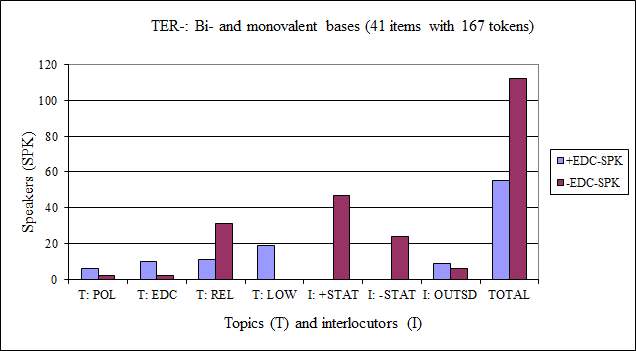
\includegraphics[scale=0.7]{./figures/Figure_3_1}
\begin{tikzpicture}
\begin{axis}[klugeaxis,title={\textscItal{ter}-: Bi- and \isi{monovalent} bases (41 items with 167 tokens)}]
\addplot[klugedots]	coordinates {(1,6)(2,10)(3,11)(4,19)(5,0)(6,0)(7,9)(8,55)};
\addplot[klugelines] coordinates {(1,2)(2,2)(3,31)(4,0)(5,47)(6,24)(7,6)(8,112)};		
\legend{\textsc{+edc-spk},\textsc{-edc-spk}}
\end{axis}
\end{tikzpicture}
\caption[Token frequencies for {ter-}prefixed lexemes with bi- and \isi{monovalent} verbal bases by speakers, topics, and interlocutors\label{Figure_3.1}]{Token frequencies for \textscItal{ter-}prefixed lexemes with bi- and \isi{monovalent} verbal bases by speakers, topics, and interlocutors\label{Figure_3.1}}
\end{figure}


The data given in \tabref{Table_3.5} and \figref{Figure_3.1} shows that for the 43 \textscItal{ter-}prefixed lexemes, most tokens (143/167 – 86\%) can be explained in terms of speaker education levels, topics, and/or role-relations between the speakers and their interlocutors; this total includes 130/153 tokens (85\%) with \isi{bivalent} bases, and 13/14 tokens (93\%) with \isi{monovalent} bases.


Only 55/167 tokens (33\%) were produced by better-educated speakers (\textsc{+edc-spk}) while most tokens (112/167 – 67\%) were produced by less-educated speakers (\textsc{-edc-spk}). The \textsc{+edc-spk} produced half of their tokens (27/55 – 49\%) during discussions about \textsc{high} topics, that is, political, educational or religious affairs (\textsc{pol}, \textsc{edc} and \textsc{rel}, respectively). Another 19 tokens (35\%) occurred during conversations with fellow-Papuans (both \textsc{+stat} and \textsc{-stat} speakers) about \textsc{low} topics. The remaining nine tokens (16\%) occurred while conversing with an outsider, namely the author (\textsc{outsd}).



The \textsc{-edc-spk} produced most of their tokens (47/112 – 42\%) while discussing \textsc{low} topics with \textsc{+stat} speakers (47 tokens). Another 35/112 tokens (31\%) were produced during discussions about \textsc{high} topics, while 6/112 tokens (5\%) occurred during conversations with the author. The remaining 24/112 tokens (21\%) occurred when \textsc{-edc-spk} discussed \textsc{low} topics with \textsc{-stat} Papuans, and therefore cannot be explained in terms of speaker education levels, topics, and/or role-relations. This total of 24 tokens refers to 14\% of all 167 \textscItal{ter-}tokens, including 23/153 tokens (15\%) with \isi{bivalent} bases and 1/14 tokens (7\%) with \isi{monovalent} bases.\footnote{As for the 21 hapaxes (17 with \isi{bivalent} and four with \isi{monovalent} bases), 18 appear to be conditioned by the variables of speaker education levels, topics, and/or role-relations, and therefore seem to be code-switches with Indonesian. This leaves only three hapaxes (with \isi{bivalent} bases) that are unaccounted for in terms of language external factors and that might result from a productive derivation process. For three hapaxes, P=0.0180 as opposed to P=0.1257 for 21 hapaxes (N=167).}


\subsubsection[Summary and conclusions]{Summary and conclusions}\label{Para_3.1.2.5}
For most of the derived verbs with \isi{bivalent} bases, the data suggests a productive form-function relationship between the derived lexemes and their bases. This conclusion is based on four observations: (1) the valency-decreasing or -reducing function of \textscItal{ter-} of removing or downplaying agent-like participants, (2) the transparent form-function relationships between derived lexemes and bases, (3) the large number of low frequency words and small number of high frequency words, and (4) the relative token frequencies with most bases having higher frequencies than the affixed lexemes.



For the prefixed verbs with \isi{monovalent} bases, the derivation process also seems to be productive, given (1) the transparent form-function relationships between derived lexemes and bases, (2) the comparatively large number of low frequency words and small number of high frequency words, and (3) the relative token frequencies with most bases having higher frequencies than the affixed lexemes. However, the low type frequency, with only five derived verbs, suggests that \textscItal{ter-}prefixation of \isi{monovalent} bases plays a minor role.



As for the speech situations during which the derived lexemes occurred, a sizable number of verbs with \isi{bivalent} bases cannot be explained in terms of pertinent variables of the \isi{communicative event}. Most tokens, however, including those with \isi{bivalent} bases, seem to be conditioned by the variables of speaker education levels, topics, and/or role-relations and therefore are best explained as code-switches with Indonesian.



These findings suggest that in Papuan Malay \textscItal{ter-}\isi{affixation} is a productive process to derive \isi{monovalent} verbs that denote accidental or unintentional actions. The degree of productivity appears to be limited, however, given that most of the attested tokens are best explained as code-switches with Indonesian.


\subsection{Suffix \textitbf{-an}\textitbf{g} ‘\textsc{pat}’}\label{Para_3.1.3}

Affixation with \textitbf{-ang} ‘\textsc{pat}’ typically derives nominals from verbal bases. The derived nouns denote the patient or result of the action, event, or state specified by the \isi{verbal base}, as illustrated in (\ref{Example_3.10}). Some lexical items are also derived from nominal and \isi{numeral} bases. The derivation process seems to be productive in Papuan Malay to some degree, as discussed below.


\ea
\label{Example_3.10}
\gll {\bluebold{pake–ang}} {itu} {basa} {smua}\\ %
 use–\textsc{pat}  \textsc{d.dist}  be.wet  all\\
\glt 
‘all those \bluebold{clothes} were wet’ \textstyleExampleSource{[080917-008-NP.0139]}
\z


Suffix \textitbf{-ang} is a reflex of Proto-\ili{Malayic} *\textitbf{-}\textscItal{a}\textitbf{n}, which “was a noun-forming suffix occurring on the basis of VTRs and denoting the goal or result of an act” \citep[174]{Adelaar.1992}. In Standard Malay, when affixed to \isi{monovalent} bases, the suffix designates “something that has the quality of” the \isi{monovalent} base, while with transitive bases it denotes the “goal or result of an action, or place where the action takes place” or “the instrument” (\citeyear*[172–173]{Adelaar.1992}). As for the \ili{eastern Malay varieties}, the suffix is only mentioned for \ili{Ambon Malay}. Also realized as \textitbf{-ang}, it “refers to the object of the transitive \isi{verb} or an instrument used in an act of V” \citep[106]{vanMinde.1997}. It is left unclear, however, whether and to what degree the \ili{Ambon Malay} suffix is productive. These observations are again an indication of the distinct history of Papuan Malay vis-à-vis the other Malay varieties, discussed in §\ref{Para_1.8}. Moreover, the similarities between Papuan Malay and \ili{Ambon Malay} reflect the link between both speech communities, also discussed in §\ref{Para_1.8}.


The corpus contains 84 nouns (441 tokens) suffixed with \textitbf{-}\textitbf{ang}:\footnote{The 84 nouns include 28 hapaxes (P=0.0635); the 69 nouns with verbal bases include 23 hapaxes (P=0.0571); the 15 nouns with nominal or \isi{numeral} bases include five hapaxes (P=0.1316).}


%\setcounter{itemize}{0}
\begin{enumerate}
\item 
Nouns with verbal bases (69 items with 403 tokens)
\item 
Nouns with nominal or \isi{numeral} bases (15 items with 38 tokens)
\end{enumerate}

The corpus also includes 28 formally complex words that have non-comp\-os\-ition\-al semantics, such as \textitbf{kasiang} ‘pity’, \textitbf{lapangang} ‘field’, or \textitbf{grakang} ‘movement’.



Suffixed items with verbal bases are examined in §\ref{Para_3.1.3.1}, and those with nominal bases in §\ref{Para_3.1.3.2}. Variables of the \isi{communicative event} that may impact the use of \textitbf{-ang} are explored in §\ref{Para_3.1.3.3}. The main findings on suffix \textitbf{-ang} are summarized and evaluated in §\ref{Para_3.1.3.4}.


\subsubsection[Suffixed items derived from verbal bases]{Suffixed items derived from verbal bases}\label{Para_3.1.3.1}

The corpus contains 69 \textitbf{-ang}{}-suffixed items (with 403 tokens) with verbal bases, including bases such as \isi{bivalent} \textitbf{pake} ‘use’, \isi{monovalent} dynamic \textitbf{jalang} ‘walk’, or \isi{monovalent} stative \textitbf{dulu} ‘be prior’. Affixation with \textitbf{-ang} typically derives nouns that denote the object of the action, event, or state indicated by the \isi{verbal base}.



Derived words with token frequencies of five or more are listed in \tabref{Table_3.6}. Most of the affixed lexemes are low frequency words (63 lexemes, attested with less than 20 tokens). Moreover, the token frequencies for the respective bases are (much) higher for most of the derived words (64 lexemes). While all 69 derived lexemes are structurally nouns, three of them have other than nominal functions in their actual uses: \textitbf{jualang} ‘merchandise’, \textitbf{duluang} ‘be prior’, and \textitbf{latiang} ‘practice'; illustrations are provided in (\ref{Example_3.13}) to (\ref{Example_3.15}).



Seven of the 69 lexemes were tentatively classified as borrowings from \ili{Standard Indonesian} (SI-borrowings) (for more details see language internal factor (\ref{List_3.1.f}) in §\ref{Para_3.1.1}, p. \pageref{List_3.1.f}). As their token frequencies are four or less, they are not included in \tabref{Table_3.6}.

\begin{table}
\caption{Affixation with \textitbf{-ang} of verbal bases}\label{Table_3.6}
\setlength{\tabcolsep}{0.6mm}
\begin{tabularx}{\textwidth}{llllrr}
\lsptoprule
 \multicolumn{1}{c}{BW} & \multicolumn{1}{c}{Gloss} & \multicolumn{1}{c}{Item} & \multicolumn{1}{c}{Gloss} & \multicolumn{1}{c}{\textitbf{-ang} \#} &  \multicolumn{1}{c}{BW \#}\\

\midrule

\textitbf{makang} & ‘eat’ & \textitbf{makangang} & ‘food’ &  57 &  414\\

\textitbf{pake} & ‘use’ & \textitbf{pakeang} & ‘clothes’ &  38 &  218\\

\textitbf{dulu} & ‘be prior’ & \textitbf{duluang} & ‘be prior to others’ &  29 &  351\\

\textitbf{bagi} & ‘divide’ & \textitbf{bagiang} & ‘part’ &  28 &  63\\

\textitbf{pikir} & ‘think’ & \textitbf{pikirang} & ‘thought’ &  23 &  102\\

\textitbf{uji} & ‘examine’ & \textitbf{ujiang} & ‘examination, examine’ &  21 &  1\\

\textitbf{lati} & ‘practice’ & \textitbf{latiang} & ‘practice’ &  17 &  3\\

\textitbf{kubur} & ‘burry’ & \textitbf{kuburang} & ‘grave’ &  14 &  8\\

\textitbf{atur} & ‘arrange’ & \textitbf{aturang} & ‘regulation’ &  8 &  24\\

\textitbf{ikat} & ‘tie up’ & \textitbf{ikatang} & ‘tie’ &  8 &  14\\

\textitbf{jual} & ‘sell’ & \textitbf{jualang} & ‘merchandise, sell’ &  8 &  14\\

\textitbf{turung} & ‘descend’ & \textitbf{turungang} & ‘descendant’ &  8 &  192\\

\textitbf{ulang} & ‘repeat’ & \textitbf{ulangang} & ‘\isi{repetition}’ &  8 &  16\\

\textitbf{bantu} & ‘help’ & \textitbf{bantuang} & ‘help’ &  7 &  34\\

\textitbf{alas} & ‘put down as base’ & \textitbf{alasang} & ‘reason’ &  6 &  7\\

\textitbf{bangun}\textitbf{g} & ‘build’ & \textitbf{bangungan}\textitbf{g} & ‘building’ &  6 &  25\\

\textitbf{libur} & ‘have vacation’ & \textitbf{liburang} & ‘vacation’ &  6 &  10\\

\textitbf{campur} & ‘mix’ & \textitbf{campurang} & ‘mixture’ &  5 &  5\\

\textitbf{jalang} & ‘walk’ & \textitbf{jalangang} & ‘route’ &  5 &  485\\

\textitbf{lapor} & ‘report’ & \textitbf{laporang} & ‘report’ &  5 &  14\\

\textitbf{tulis} & ‘write’ & \textitbf{tulisang} & ‘writing’ &  5 &  12\\

\lspbottomrule
\end{tabularx}
\end{table}

Affixing verbal bases with \textitbf{-ang} typically derives nouns that denote the object of the action specified by the \isi{verbal base}. The suffixed nouns include patients such as \textitbf{makangang} ‘that which is eaten’ or ‘food’, or results such as \textitbf{bagiang} ‘that which is divided’ or ‘part’. “Objective nominalization” that derives “nouns designating the result, or the typical or ‘cognate’ object of an action” has also been observed for other languages \citep[340]{Comrie.2007}. This polysemy can be explained in terms of a “domain shift” in that “one may go from one semantic domain to another, related one, and thus derive new interpretations” {\citep[221]{Booij.2007}}. Hence, suffix \textitbf{-ang} is glossed as ‘\textsc{pat}’ (‘patient’) in the sense of ‘patients or results which are \textsc{base}{}-ed’.


Two derived nouns together with their bases are given in context: \textitbf{makangang} ‘food’ with its \isi{bivalent} base \textitbf{makang} ‘eat’ in (\ref{Example_3.11}), and \textitbf{jalangang} ‘route’ with its \isi{monovalent} base \textitbf{jalang} ‘walk’ in (\ref{Example_3.12}).


\newpage
\begin{styleExampleTitle}
{Suffix \textitbf{-ang}: Semantics of verbal bases and derived lexemes}
\end{styleExampleTitle}

\ea
\label{Example_3.11}
\gll {maytua} {bilang,} {\bluebold{makang}} {karna} {\bluebold{makang–ang}} {suda} {masak}\\ %
 wife  say  eat  because  eat–\textsc{pat}  already  cook\\
\glt 
‘(my) wife said, ``\bluebold{eat}, because the \bluebold{food} has already been cooked''’ \textstyleExampleSource{[080919-004-NP.0039]}
\z

\ea
\label{Example_3.12}
\gll {{trus}} {kitong} {dua} {{pulang,}} {{sampe}} {di} {\bluebold{jalang–ang}} {sa} {istirahat,}\\ %
 {next}  \textsc{1pl}  two  {go.home}  {reach}  at  walk–\textsc{pat}  \textsc{1sg}  rest\\
\gll  de  {bilang,}  {kitong}  dua  {\bluebold{jalang}}  {suda!}\\
 \textsc{3sg}  {say}  {\textsc{1pl}}  two  {walk}  {already}\\
\glt 
‘and then we two went home, on the \bluebold{way} I rested, he said, ``let the two of us \bluebold{walk} (on)!''’ \textstyleExampleSource{[081015-005-NP.0036]}
\z


Some of the suffixed items, listed in \tabref{Table_3.6}, differ from the other suffixed items, as for example \textitbf{jual-ang} ‘sell-\textsc{pat}’ and \textitbf{dulu-ang} ‘be.prior-\textsc{pat}’. Suffixed with \textitbf{-ang}, these items are structurally nouns. In a sentence, however, \textitbf{jualang} also functions as the \isi{verb} ‘sell’ in the same way as its base \textitbf{jual} ‘sell’, as shown in (\ref{Example_3.13}). Likewise \textitbf{duluang} ‘be.prior-\textsc{pat}’ in (\ref{Example_3.14}) is used in the same way as its base \textitbf{dulu} ‘be prior’ in (\ref{Example_3.15}).



\begin{styleExampleTitle}
%\caption
{Suffix \textitbf{-ang}: Verbal reading of derived lexemes}
\end{styleExampleTitle}

\ea
\label{Example_3.13}
\gll {mama} {saya} {pergi} {\bluebold{jual}} {pinang,} {sa} {pu} {mama} {\bluebold{jual–ang}}\\ %
 mother  \textsc{1sg}  go  sell  betel.nut  \textsc{1sg}  \textsc{poss}  mother  sell–\textsc{pat}\\
\gll {pinang}\\
 {betel.nut}\\
\glt 
‘my mother went to \bluebold{sell} betel nuts, my mother \bluebold{sells} betel nuts’ \textstyleExampleSource{[081014-014-NP.0002]}
\z

\ea
\label{Example_3.14}
\gll {nanti} {kam} {dari} {blakang,} {bapa} {\bluebold{dulu–ang}}\\ %
 very.soon  \textsc{2pl}  from  backside  father  be.prior–\textsc{pat}\\

\glt
[About an upcoming official meeting:] ‘then you two (go in) second, (and) the gentleman \bluebold{(goes) ahead}’ \textstyleExampleSource{[081011-001-Cv.0199]}

\z
\ea
\label{Example_3.15}
\gll {dua} {orang} {\bluebold{dulu}}\\ %
 two  person  be.prior\\
\glt
[About the number of potential nominees for the upcoming local election:] ‘two people \bluebold{(go) ahead}’ \textstyleExampleSource{[080919-001-Cv.0065]}
\z

\subsubsection[Suffixed items derived from nominal or {numeral} bases]{Suffixed items derived from nominal or {numeral} bases}\label{Para_3.1.3.2}
The corpus contains 13 \textitbf{-ang}{}-suffixed lexemes with nominal bases (36 tokens) and two derived lexemes with \isi{numeral} bases (2 tokens), as listed in \tabref{Table_3.7}. In most cases, the bases and the derived nouns differ in their semantics. In some cases, the affixed nouns designate a magnification of the base, such as \textitbf{laut} ‘sea’ and \textitbf{lautang} ‘ocean’, or \textitbf{ruang} ‘room’ and \textitbf{ruangang} ‘large room’. In some cases, the meanings of the derived nouns are an extension of the meanings of their bases with suffix \textitbf{-ang} having a generalizing function, as for instance \textitbf{ana} ‘child’ and \textitbf{anaang} ‘offspring’, or \textitbf{musim} ‘season’ and \textitbf{musimang} ‘each season’. In yet other cases, the affixed nouns have unpredictable meanings compared to the semantics of their bases, such as \textitbf{rambut} ‘hair’ and \textitbf{rambutang} ‘rambutan’, or \textitbf{obat} ‘medicine’ and \textitbf{obatang} ‘magic spell’. And in a few cases, the base and the derived \isi{noun} have the same semantics, as in \textitbf{pasang} ‘pair’ and \textitbf{pasangang} ‘pair’ or \textitbf{pangkal} ‘base’ and \textitbf{pangkalang} ‘base’.



All 13 derived lexemes are low frequency words, attested with less than 20 tokens. Moreover, the token frequencies for the respective bases are (much) higher for most of the derived words (10 lexemes); for one lexeme, the base is unattested in the corpus, although it does exist. Four of the 15 derived nouns were tentatively classified as SI-borrowings; in \tabref{Table_3.7} these items are underlined (for more details see language internal factor (\ref{List_3.1.f}) in §\ref{Para_3.1.1}, p. \pageref{List_3.1.f}).

\begin{table}

\caption{Affixation with \textitbf{-ang} of nominal and \isi{numeral} bases}\label{Table_3.7}
\begin{tabularx}{\textwidth}{lXXXrr}
\lsptoprule

 \multicolumn{1}{c}{BW} & \multicolumn{1}{c}{Gloss} & \multicolumn{1}{c}{Item} & \multicolumn{1}{c}{Gloss} & \multicolumn{1}{c}{\textitbf{-ang} \#} & \multicolumn{1}{c}{ BW \#}\\

\midrule
\textitbf{bayang} & ‘image’ & \textitbf{bayangang} & ‘shadow’ &  6 &  2\\

\textitbf{ana} & ‘child’ & \textitbf{anaang} & ‘offspring’ &  4 &  741\\

\textitbf{tingkat} & ‘floor’ & \textitbfUndl{tingkatang} & ‘level’ &  4 &  5\\

\textitbf{hukum} & ‘law’ & \textitbf{hukumang} & ‘punishment’ &  4 &  3\\

\textitbf{rambut} & ‘hair’ & \textitbf{rambutang} & ‘rambutan’ &  3 &  23\\

\textitbf{obat} & ‘medicine’ & \textitbf{obatang} & ‘magic spell’ &  3 &  9\\

\textitbf{pasang} & ‘pair’ & \textitbf{pasangang} & ‘pair’ &  3 &  2\\

\textitbf{laut} & ‘sea’ & \textitbf{lautang} & ‘ocean’ &  2 &  68\\

\textitbf{pinggir} & ‘border’ & \textitbfUndl{pinggirang} & ‘edges’ &  2 &  23\\

\textitbf{ruang} & ‘room’ & \textitbf{ruangang} & ‘large room’ &  2 &  3\\

\textitbf{kandung} & ‘womb’ & \textitbfUndl{kandungang} & ‘womb’ &  1 &  8\\

\textitbf{musim} & ‘season’ & \textitbfUndl{musimang} & ‘each season’ &  1 &  5\\

\textitbf{pangkal} & ‘base’ & \textitbf{pangkalang} & ‘base’ &  1 &  0\\

\textitbf{pulu} & ‘tens’ & \textitbf{puluang} & ‘tens’ &  1 &  78\\

\textitbf{ratus} & ‘hundreds’ & \textitbf{ratusang} & ‘hundreds’ &  1 &  34\\

\lspbottomrule
\end{tabularx}
\end{table}

The data listed in \tabref{Table_3.7} shows that most of the nominal bases and affixed nouns differ in their semantics. The magnifying function of suffix \textitbf{-ang} is illustrated in (\ref{Example_3.16}) and (\ref{Example_3.17}), the generalizing function in (\ref{Example_3.18}), and its unpredictable semantics in (\ref{Example_3.19}) and (\ref{Example_3.20}).


The magnifying function of \textitbf{-ang} is demonstrated with \textitbf{laut} ‘sea’ in (\ref{Example_3.16}) and \textitbf{lautang} ‘ocean’ in (\ref{Example_3.17}). While \textitbf{laut} refers to the ‘sea’ close to the coast, \textitbf{lautang} denotes the open and deep ‘ocean’ off the coast.

\newpage

\begin{styleExampleTitle}
{Suffix \textitbf{-ang}: Magnifying function}
\end{styleExampleTitle}

\ea
\label{Example_3.16}
\gll {dong} {dua} {pergi} {mancing} {di} {\bluebold{laut}}\\ %
 \textsc{3pl}  two  go  fish.with.rod  at  sea\\
\glt 
‘the two of them went fishing on the \bluebold{sea}’ \textstyleExampleSource{[081109-005-JR.0005]}
\z
\ea
\label{Example_3.17}
\glll {banyak} {mati} {\ldots} {di} {pulow{\Tilde}pulow} {banyak} {mati} {di} \bluebold{laut–ang}\\ %
{} {} {} {} {} {} {} {} {sea–\textsc{pat}}\\
 many  die {}   at  \textsc{rdp}{\Tilde}island  many  die  at  ocean\\
\glt ‘many died {\ldots} on the islands, many died on the (open) \bluebold{ocean}’ \textstyleExampleSource{[081029-002-Cv.0025]}
\z
%\todo[inline]{Please check this example.}

The generalizing function of \textitbf{-ang} is illustrated with \textitbf{ana} ‘child’ and \textitbf{anaang} ‘offspring’ in (\ref{Example_3.18}).



\begin{styleExampleTitle}
{Suffix \textitbf{-ang}: Generalizing function}
\end{styleExampleTitle}
\ea
\label{Example_3.18}
\gll {kalo} {{mo}} {antar} {{\bluebold{ana}}} {{\bluebold{prempuang}}} {ke} {\bluebold{ana}} {{\bluebold{laki{\Tilde}laki}}} {{\ldots}} {kitorang}\\ %
 if  {want}  bring  {child}  {woman}  to  child  {\textsc{rdp}{\Tilde}husband}  {}  \textsc{1pl}\\
 
 \glll {itu}  {harus}  {\ldots}  {bawa}  \bluebold{ana–ang}  {pinang}  \bluebold{ana–ang}  {sagu}\\
 {} {} {} {} child–\textsc{pat} {} child–\textsc{pat} {} \\
  {\textsc{d.dist}} {have.to} {}   {bring}  {offspring}  {betel.nut}  {offspring}  {sago}\\
\glt 
[About wedding preparations:] ‘if we want to bring our \bluebold{daughter} to (their) \bluebold{son} {\ldots} we have to {\ldots} bring betel nut \bluebold{seedlings} (and) sago \bluebold{seedlings}’ (Lit. ‘female/male \bluebold{child}; betel nut/sago \bluebold{offspring}’) \textstyleExampleSource{[081110-005-CvPr.0055-0057]}
\z
%\todo[inline]{Please check this example.}


In some cases, the semantics of the affixed nouns are unpredictable, although a connection between the base word and the derived word can still be seen. This is demonstrated with \textitbf{rambut} ‘hair’ in (\ref{Example_3.19}) and \textitbf{rambutang} ‘rambutan’ in (\ref{Example_3.20}), which refers to the fruit of the rambutan tree (\textstyleChItalic{Nephelium lappaceum}). The leathery reddish skin of the fruit is covered with numerous hairy protuberances, which is depicted by the label \textitbf{rambut-ang} ‘hair-\textsc{pat}’.



\begin{styleExampleTitle}
{Suffix \textitbf{-ang}: Unpredictable semantics}
\end{styleExampleTitle}

\ea
\label{Example_3.19}
\gll {sa} {mo} {cuci} {de} {pu} {\bluebold{rambut}}\\ %
 \textsc{1sg}  want  wash  \textsc{3sg}  \textsc{poss}  hair\\
\glt 
‘I want to wash her \bluebold{hair}’ \textstyleExampleSource{[081025-001-CvHt.0006]}
\z

\ea
\label{Example_3.20}
\glll {di} {sini} {ada} {jambu} {di} {sini} {ada} {ada} \bluebold{rambut–ang}\\ %
 {} {} {} {} {} {} {} {} hair–\textsc{pat}\\
 at  \textsc{l.prox}  exist  rose.apple  at  \textsc{l.prox}  exist  exist  rambutan\\
\glt
‘here are rose apples, here are are \bluebold{rambutan}’ \textstyleExampleSource{[081029-001-Cv.0006]}
\z
%\todo[inline]{Please check this example.}

\subsubsection[Variables of the {communicative event}]{Variables of the communicative event}\label{Para_3.1.3.3}

To further investigate the issue of productivity of \textitbf{-ang} in Papuan Malay, a domain analysis was conducted which focused on the variables of speaker education levels, topics, and/or role-relations (for details see ``Language external factors'' in §\ref{Para_3.1.1}, p. \pageref{List_3.2}). In all, 84 items suffixed with \textitbf{-ang}, totaling 441 tokens, were investigated:


\begin{itemize}
\item 
69 suffixed items derived from verbal bases (403 tokens)

\item 
15 suffixed items derived from nominal or \isi{numeral} bases (38 tokens)

\end{itemize}

For the 84 suffixed lexemes, 352/441 tokens (80\%) can be accounted for in terms of speaker education levels, topics, and/or role-relations. The remaining 89/441 tokens (20\%) occurred when less-educated speakers (\textsc{-edc-spk}) talked with fellow-Papuans of equally low social standing (\textsc{-stat}) about \textsc{low} topics.\footnote{As mentioned under Factor 3 ``Relationships between interlocutors'' in §\ref{Para_1.5.1} (p. \pageref{Item_1.3}), all of the recorded less-educated speakers belong to the group of Papuans with lower social status (\textsc{-stat}), while the recorded Papuans with higher social status (\textsc{+stat}), such as teachers, government officials, or pastors, are all better educated.} (See \tabref{Table_3.8} and \figref{Figure_3.2}.)



That is, a considerable number of tokens (20\%) cannot be explained in terms of these variables of the \isi{communicative event}. Therefore, it cannot be concluded that the respective lexemes are code-switches with Indonesian. This total of 89/441 tokens (20\%) includes 80/403 tokens (20\%) with verbal bases and 9/38 tokens (24\%) with nominal or \isi{numeral} bases. The vast majority of \textitbf{-ang}{}-suffixed tokens (352/441 – 80\%), however, seem to be conditioned by variables of the \isi{communicative event}.



As for the rather high number of unaccounted tokens with nominal or \isi{numeral} bases (9/38 – 24\%), one observation is made. Four of the nine tokens refer to the same lexeme produced by the same speaker during three conversations about the same topic, namely the death of a young mother. This speaker has a reputation of speaking incoherently due to his unsuccessful attempts to approximate \ili{Standard Indonesian}. Excluding these four tokens brings down the number of unaccounted lexemes to 15\% (5/34). If \isi{affixation} of nominal bases was a productive process, however, one would expect this percentage to be much higher. In turn, this finding does not support the conclusion that the suffixed lexemes with nominal or \isi{numeral} bases result from a productive derivation process. Instead, they seem to be code-switches with Indonesian.



The data presented in \tabref{Table_3.8} and \figref{Figure_3.2} is discussed in more detail below.

\begin{table}
\caption{Token frequencies for \textitbf{-ang}{}-suffixed lexemes with verbal, nominal, and \isi{numeral} bases by speakers, topics, and interlocutors (84 items)}\label{Table_3.8}

\begin{tabular}{lllllllll}
\lsptoprule

 & \multicolumn{4}{l}{ Topics (\textsc{top})} & \multicolumn{3}{l}{ Interlocutors (\textsc{ilct})} &  Tokens\\
\midrule
\multicolumn{9}{l}{Suffixed lexemes with verbal bases (69 items)}\\
\midrule
& \textsc{pol} & \textsc{edc} & \textsc{rel} & \textsc{low} & \textsc{+stat} & \textsc{-stat} & \textsc{outsd} &  Total\\

\textsc{+edc-spk} &  30 &  26 &  15 &  46 &  {}-{}-{}- &  {}-{}-{}- &  75 &  192\\

\textsc{-edc-spk} &  15 &  40 &  47 &  {}-{}-{}- &  26 &  \textstyleChBold{80} &  3 &  211\\

Subtotal &  45 &  66 &  62 &  46 &  26 &  \textstyleChBold{80} &  78 &  403\\
\midrule
\multicolumn{9}{l}{Suffixed lexemes with nominal and \isi{numeral} bases (15 items)}\\
\midrule

& \textsc{pol} & \textsc{edc} & \textsc{rel} & \textsc{low} & \textsc{+stat} & \textsc{-stat} & \textsc{outsd} &  Total\\

\textsc{+edc-spk} &  4 &  1 &  0 &  4 &  {}-{}-{}- &  {}-{}-{}- &  8 &  17\\

\textsc{-edc-spk} &  3 &  0 &  6 &  {}-{}-{}- &  1 &  \textstyleChBold{9} &  2 &  20\\

Subtotal &  7 &  1 &  6 &  4 &  1 &  \textstyleChBold{9} &  10 &  38\\
\midrule
\multicolumn{9}{l}{\textstyleChBold{TOTAL} (84 items)}\\
\midrule
& \textsc{pol} & \textsc{edc} & \textsc{rel} & \textsc{low} & \textsc{+stat} & \textsc{-stat} & \textsc{outsd} &  Total\\

\textsc{+edc-spk} &  34 &  27 &  15 &  50 &  {}-{}-{}- &  {}-{}-{}- &  83 &  209\\

\textsc{-edc-spk} &  18 &  40 &  53 &  {}-{}-{}- &  27 &  \textstyleChBold{89} &  5 &  232\\
\midrule
\textstyleChBold{Total} &  52 &  67 &  68 &  50 &  27 &  \textstyleChBold{89} &  88 &  \textstyleChBold{441}\\

\lspbottomrule
\end{tabular}
\end{table}
\begin{figure}
\centering
%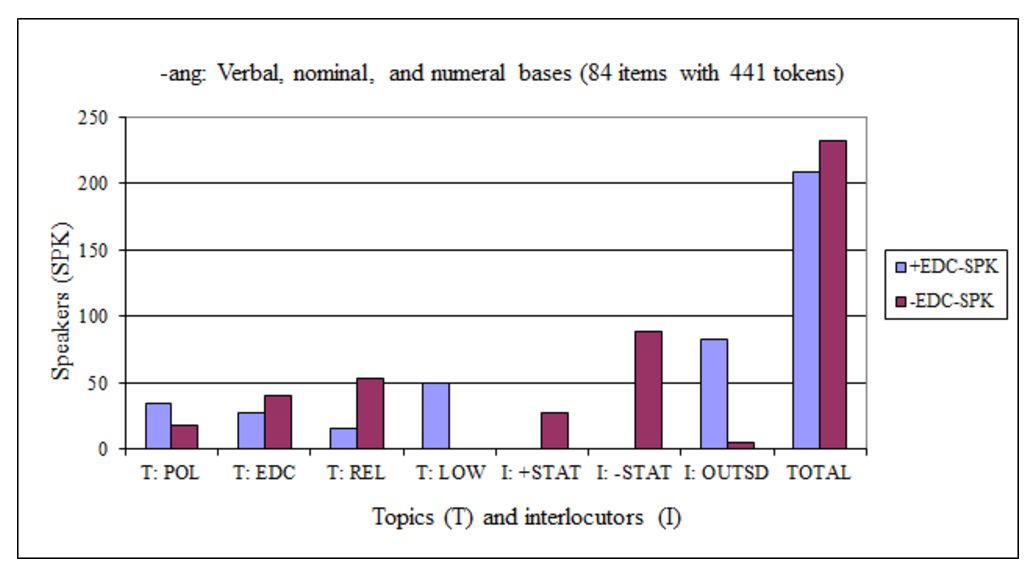
\includegraphics[scale=0.7]{./figures/Figure_3_2}
\begin{tikzpicture}
\begin{axis}[klugeaxis, y={}, height={.5\textheight}, title={\textitbf{-ang}: Verbal, nominal, and \isi{numeral} bases (84 items with 441 tokens)}]
\addplot[klugedots]	coordinates {(1,34)(2,27)(3,15)(4,50)(5,0)(6,0)(7,83)(8,209)};
\addplot[klugelines] coordinates {(1,18)(2,40)(3,53)(4,0)(5,27)(6,89)(7,5)(8,232)};		
\legend{\textsc{+edc-spk},\textsc{-edc-spk}}
\end{axis}
\end{tikzpicture}
\caption{Token frequencies for \textitbf{-ang}{}-suffixed lexemes with verbal, nominal, and \isi{numeral} bases by speakers, topics, and interlocutors\label{Figure_3.2}}
\end{figure}

The data given in \tabref{Table_3.8} and \figref{Figure_3.2} shows that for the 84 \textitbf{-ang}{}-suffixed lexemes, 352/441 tokens (80\%) can be explained in terms of speaker education levels, topics, and/or role-relations between the speakers and their interlocutors; this includes 323/403 tokens (80\%) with verbal bases, and 29/38 tokens (76\%) with nominal bases.


The better-educated speakers (\textsc{+edc-spk}) produced 209/441 tokens (47\%), while the less-educated speakers (\textsc{-edc-spk}) produced 232/441 (53\%) tokens.



In terms of topics (\textsc{top}), 187/441 tokens (42\%) occurred during conversations about \textsc{high} topics, that is, political, educational or religious affairs (\textsc{pol}, \textsc{edc} and \textsc{rel}, respectively). This includes 76/209 \textsc{+edc-spk} tokens (36\%) and 111/232 \textsc{-edc-spk} tokens (48\%). 
Another 88/441 tokens (20\%) were produced in conversations with an outsider, namely the author (\textsc{outsd}), including 83/209 \textsc{+edc-spk} tokens (40\%) and 5/232 \textsc{-edc-spk} tokens (0.2\%).



This leaves 166/441 tokens (38\%) that were produced when the interlocutors discussed \textsc{low} topics. This includes 50/166 \textsc{+edc-spk} tokens (30\%) and 116/166 \textsc{-edc-spk} tokens (70\%). The 116 \textsc{low} topic tokens produced by \textsc{-edc-spk} are distributed as follows. When conversing with \textsc{+stat} Papuans, 27 tokens were produced (that is, 27/232 \textsc{-edc-spk} tokens – 12\%). The remaining 89 tokens (that is, 89/232 \textsc{-edc-spk} tokens – 38\%) occurred when \textsc{-edc-spk} discussed \textsc{low} topics with \textsc{-stat} Papuans, and therefore cannot be explained in terms of speaker education levels, topics, and/or role-relations. This total of 89 tokens refers to 20\% of all 441 \textitbf{-ang} tokens. It includes 80/403 tokens (20\%) with verbal bases and 9/38 tokens (24\%) with nominal or \isi{numeral} bases.\footnote{As for the 28 hapaxes (23 with verbal bases, and five with nominal bases), 17 appear to be conditioned by the variables of speaker education levels, topics, and/or role-relations, and therefore are best explained as code-switches with Indonesian. This leaves 11 hapaxes that are unaccounted for in terms of language external factors and that might be the result of a productive \isi{word-formation} process. For 11 hapaxes, P=0.0249 as opposed to P=0.0635 for 28 hapaxes (N=441). The total of 11 hapaxes includes nine with verbal bases (P=0.0223) and two with nominal or \isi{numeral} bases (P=0.0526).}


\subsubsection[Summary and conclusions]{Summary and conclusions}\label{Para_3.1.3.4}

Suffix \textitbf{-ang} is polyfunctional in that it derives nouns from verbal, nominal, and \isi{numeral} bases. This polyfunctionality suggests that \isi{affixation} with \textitbf{-ang} is a somewhat productive process (see language internal factor (\ref{List_3.1.c}) in §\ref{Para_3.1.1}, p. \pageref{List_3.1.c}).



Concerning \textitbf{-ang}{}-\isi{affixation} of verbal bases, four other observations support this conclusion: (1) the transparent form-function relationship between the derived nouns and their respective bases, (2) the large number of low frequency words and small number of high frequency words, (3) the relative token frequencies with most bases having higher frequencies than the affixed lexemes, and (4) the low number of derived lexemes tentatively classified as SI-borrowings.



To a lesser extent, the same observations apply to \textitbf{-ang}{}-\isi{affixation} of nominal bases: (1) the form-function relationships between derived lexemes and bases is more or less transparent, (2) all derived lexemes are low frequency words, (3) most bases have higher token frequencies than the affixed lexemes, and (3) the number of derived lexemes tentatively classified as SI-borrowings is rather low. These findings suggest that \textitbf{-ang}{}-\isi{affixation} of nominal bases is also a somewhat productive process.



With respect to the speech situations during which the derived nouns occurred, the following patterns emerge. For affixed nouns with verbal bases, one fifth of the attested tokens cannot be accounted for in terms of pertinent variables of the \isi{communicative event}; that is, for these items there are no indications that they are code-switches with Indonesian. However, the vast majority of tokens with verbal bases (80\%) seem to be conditioned by the variables of speaker education levels, topics, and/or role-relations and are best explained as code-switches with Indonesian. The same applies to nouns with nominal bases for which most tokens also appear to be conditioned by the three mentioned variables of the \isi{communicative event}. Hence, these items are also best explained as code-switches with Indonesian.



These findings suggest that in Papuan Malay \textitbf{-ang}{}-\isi{affixation} is a productive process to derive nouns from verbal and nominal bases. The degree of productivity appears to be limited, however, as most tokens seem to be code-switches with Indonesian.


\subsection[Prefix {\PEN}- ‘\textsc{ag}’]{Prefix \textscItal{pe(n)}- ‘\textsc{ag}’}\label{Para_3.1.4}

Affixation with \textscItal{pe(n)}- ‘\textsc{ag}’ typically derives nominals from verbal bases. The derived nouns denote the agent or instrument of the action, event, or state specified by the \isi{verbal base}, as in (\ref{Example_3.21}). Some lexemes are also derived from nominal bases. The \isi{affixation} process appears to be marginally productive in Papuan Malay, at best, as discussed below.


\ea
\label{Example_3.21}
\gll {pokoknya} {orang} {\bluebold{pen–datang}} {pulang}\\ %
 the.main.thing.is  person  \textsc{ag}–come  go.home\\
\glt 
‘the main thing is (that) the \bluebold{strangers} return home’ (Lit. ‘\bluebold{the one who comes}’) \textstyleExampleSource{[081029-005-Cv.0048]}
\z


Suffix \textscItal{pe(n)-} is a reflex of Proto-\ili{Malayic} *\textitbf{p}\textscItal{an}\textitbf{-}, which “formed deverbal nouns that were used attributively, predicatively, and in prepositional phrases, and that had a nominal as head or subject. They denoted a purpose or instrument when prefixed to VDIs and VTRs. Moreover, *\textitbf{p}\textscItal{an}\textitbf{-} denoted an inclination or characteristic when prefixed to VSIs” \citep[193]{Adelaar.1992}. In Standard Malay, derived lexemes with a \isi{monovalent} base “denote a characteristic” while forms with a \isi{bivalent} base “usually denote an actor or instrument” or “a goal or result, or they form an abstract \isi{noun}. Furthermore \textitbf{pa}\textscItal{n}\textitbf{-} forms are used attributively, and, on the basis of VSIs, they can function as VSIs” (\citeyear*[183]{Adelaar.1992}).



In some of the \ili{eastern Malay varieties}, the prefix is also found. In \ili{Ambon Malay}, the prefix occurs but it is unproductive \citep[109]{vanMinde.1997}. In \ili{Manado Malay} \textitbf{paŋ-} also occurs and is productive (in addition, a unproductive form \textitbf{pa}\textsc{-} exists) \citep[18, 24]{Stoel.2005}. Likewise, in North Moluccan / \ili{Ternate Malay} \textitbf{pa(}\textscItal{n}\textitbf{)-} occurs, but its status is uncertain. While {\citet[4]{Voorhoeve.1983}} maintains that it “is no longer morphologically distinct”, \citet[30]{Litamahuputty.2012} states that the prefix is productive. In these varieties, the prefix usually denotes the actor or instrument of the event expressed by the base. In addition, however, some of prefixed forms can also receive a verbal reading, as discussed in more detail in §\ref{Para_3.1.4.2}.



The corpus contains 34 nouns (186 tokens) prefixed with \textscItal{pe(n)-}:\footnote{The 34 nouns include 11 hapaxes (P=0.0591); the 29 nouns with verbal bases include nine hapaxes (P=0.0588); the five nouns with nominal bases include two hapaxes (P=0.0606).}


\begin{enumerate}
\item 
Nouns with verbal bases (29 items with 153 tokens)
\item 
Nouns with nominal bases (five items with 33 tokens)
\
\end{enumerate}

The corpus also contains nine formally complex words with non-compositional semantics, such as \textitbf{peserta} ‘participant’ or \textitbf{panggayu} ‘(a/to) paddle’.



Before discussing \textscItal{pe(n)-}\isi{affixation} of verbal bases in §\ref{Para_3.1.4.2} and of nominal bases in §\ref{Para_3.1.4.3}, the \isi{allomorphy} of \textscItal{pe(n)-} is investigated in §\ref{Para_3.1.4.1}. Variables of the \isi{communicative event} that may impact the use of \textscItal{pe(n)-} are explored in §\ref{Para_3.1.4.4}. The main points on prefix \textscItal{pe(n)-} are summarized and evaluated in §\ref{Para_3.1.4.5}.


\subsubsection[Allomorphy of pe(n)-]{Allomorphy of \textscItal{pe(n)-}}\label{Para_3.1.4.1}

Prefix \textscItal{pe(n)-} has two allomorphs, \textitbf{pe(}\textscItal{n}\textitbf{)}\textitbf{-} and \textitbf{pa(}\textscItal{n}\textitbf{)}\textitbf{-} (small-caps \textscItal{n} represents the different realizations of the nasal). The allomorphs are not governed by phonological processes.



The form \textitbf{pe(}\textscItal{n}\textitbf{)}\textitbf{-}, in turn, has seven allomorphs that result from morphologically conditioned phonological rules. More specifically, they are conditioned by the word-initial segment of the base word, as shown in \tabref{Table_3.9}: /\textstyleChCharisSIL{pɛm-}/, /\textstyleChCharisSIL{pɛn-}/, /\textstyleChCharisSIL{pɛɲ-}/, \textstyleChCharisSIL{pɛŋ-}/, /\textstyleChCharisSIL{pɛ-}/, /\textstyleChCharisSIL{p-}/, and /\textstyleChCharisSIL{pl-}/. The prefix is realized as /\textstyleChCharisSIL{pɛm-}/ when the initial segment of the base is a bilabial stop. Onset voiced stops are retained, while voiceless stops are deleted. With onset bilabial /\textstyleChCharisSIL{m}/, the prefix is realized as /\textstyleChCharisSIL{pɛ-}/. With alveolar stops, the prefix is very commonly realized as /\textstyleChCharisSIL{pɛn-}/. Again, the onset voiced stop is retained, while the onset voiceless stop is deleted. Alternatively, however, the onset voiceless stop can also be retained, in which case the prefix is realized as /\textstyleChCharisSIL{pɛ-}/. With onset fricative /\textstyleChCharisSIL{s}/, the prefix is realized as /\textstyleChCharisSIL{pɛɲ-}/, with /\textstyleChCharisSIL{s}/ being deleted. With onset palato-alveolar affricates, \textitbf{pe(}\textscItal{n}\textitbf{)}\textitbf{-} is realized as /\textstyleChCharisSIL{pɛn-}/. With onset rhotic /r/, the affix is realized as /\textstyleChCharisSIL{pɛ-}/. With onset velar stops and onset vowels, the prefix is realized as /\textstyleChCharisSIL{pɛŋ-}/. Finally, when prefixed to \textitbf{ajar} ‘teach’, \textitbf{pe(}\textscItal{n}\textitbf{)}\textitbf{-} is realized as /\textstyleChCharisSIL{pl-}/.

\begin{table}
\caption[Realizations of allomorph \textitbf{pe(n)-}]{Realizations of allomorph \textitbf{pe(}\textscItal{n}\textitbf{)}\textitbf{-}}\label{Table_3.9}


\begin{tabular}{lll}
\lsptoprule

 \multicolumn{1}{c}{\textitbf{pe(}\textscItal{n}\textitbf{)-}base} & \multicolumn{1}{c}{Orthogr.} &  \multicolumn{1}{c}{Gloss}\\

\midrule
/\textstyleChCharisSIL{pɛm}–\textstyleChCharisSIL{bantu}/ & \textitbf{pembantu} & ‘house helper’\\

/\textstyleChCharisSIL{pɛm}–\textstyleChCharisSIL{pili}/ & \textitbf{pemili} & ‘voter’\\

/\textstyleChCharisSIL{pɛ}–\textstyleChCharisSIL{muda}/ & \textitbf{pemuda} & ‘youth’\\

/\textstyleChCharisSIL{pɛn}–\textstyleChCharisSIL{dataŋ}/ & \textitbf{pendatang} & ‘newcomer’\\

/\textstyleChCharisSIL{pɛn}–\textstyleChCharisSIL{tumpaŋ}/ & \textitbf{penumpang} & ‘passenger’\\

/\textstyleChCharisSIL{pɛ}–\textstyleChCharisSIL{tugas}/ & \textitbf{petugas} & ‘official’\\

/\textstyleChCharisSIL{pɛɲ}–\textstyleChCharisSIL{sakit}/ & \textitbf{penyakit} & ‘disease’\\

/\textstyleChCharisSIL{pɛn}–\textstyleChCharisSIL{tʃuri}/ & \textitbf{pencuri} & ‘thief, to steal (\textsc{emph})’\\

/\textstyleChCharisSIL{pɛn}–\textstyleChCharisSIL{dʒaga}/ & \textitbf{penjaga} & ‘guard’\\

/\textstyleChCharisSIL{pɛ}–\textstyleChCharisSIL{rɛntʃana}/ & \textitbf{perencana} & ‘planner’\\

/\textstyleChCharisSIL{pɛŋ–acara}/ & \textitbf{pengacara} & ‘master of ceremony’\\

/\textstyleChCharisSIL{pɛŋ}–\textstyleChCharisSIL{ganti}/ & \textitbf{pengganti} & ‘replacement’\\

/\textstyleChCharisSIL{pl}–\textstyleChCharisSIL{adʒar}/ & \textitbf{plajar} & ‘teacher’\\

\lspbottomrule
\end{tabular}
\end{table}

The allomorph \textitbf{pa(}\textscItal{n}\textitbf{)}\textitbf{-} occurs considerably less frequently. Attested are only the four items listed in \tabref{Table_3.10} with a total of 18 \textitbf{pa(}\textscItal{n}\textitbf{)}\textitbf{-} tokens. Form \textitbf{pa(}\textscItal{n}\textitbf{)}\textitbf{-} has two attested allomorphs: /\textstyleChCharisSIL{pan-}/ and /\textstyleChCharisSIL{pa-}/. The phonological processes involved in the \isi{allomorphy} are the same as those for \textitbf{pe(}\textscItal{n}\textitbf{)}\textitbf{-}, discussed above. For two of the items, the prefix is alternatively realized as allomorph \textitbf{pe(}\textscItal{n}\textitbf{)}\textitbf{-}. Therefore, for each item the token frequencies for \textitbf{pa(}\textscItal{n}\textitbf{)}\textitbf{-} and for \textitbf{pe(}\textscItal{n}\textitbf{)}\textitbf{-} are given. If the prefix is realized with /\textstyleChCharisSIL{pɛ(}\textsc{n}\textstyleChCharisSIL{)-}/ in a greater number of tokens than with /\textstyleChCharisSIL{pa(}\textsc{n}\textstyleChCharisSIL{)-}/, then its orthographic representation is \textscItal{pe(n)-} as in \textitbf{pencuri} ‘thief, steal (\textsc{emph})’.

\begin{table}
\caption[Realizations of allomorph \textitbf{pa(n)-}]{Realizations of allomorph \textitbf{pa(}\textscItal{n}\textitbf{)}\textitbf{-}}\label{Table_3.10}


\begin{tabularx}{\textwidth}{llXll}
\lsptoprule

 \textitbf{pa(}\textscItal{n}\textitbf{)}\textitbf{{}-}base & Orthogr. & \multicolumn{1}{c}{Gloss} & \textitbf{pa(}\textscItal{n}\textitbf{)}\textitbf{-} \# &  \textitbf{pe(}\textscItal{n}\textitbf{)}\textitbf{-} \#\\
\midrule
/\textstyleChCharisSIL{pa}–\textstyleChCharisSIL{malas}/ & \textitbf{pamalas} & ‘listless person, be very listless’ &  12 &  2\\

/\textstyleChCharisSIL{pan}–\textstyleChCharisSIL{diam}/ & \textitbf{pandiam} & ‘taciturn person, be very quiet’ &  2 &  0\\

/\textstyleChCharisSIL{pan}–\textstyleChCharisSIL{takut}/ & \textitbf{panakut} & ‘coward, be very fearful (of)’ &  3 &  0\\

/\textstyleChCharisSIL{pan}–\textstyleChCharisSIL{tʃuri}/ & \textitbf{pencuri} & ‘thief, steal (\textsc{emph})’ &  1 &  11\\

\lspbottomrule
\end{tabularx}
\end{table}

In realizing the prefix typically as \textitbf{pe(}\textscItal{n}\textitbf{)}\textitbf{-} rather than as \textitbf{pa(}\textscItal{n}\textitbf{)}\textitbf{-}, Papuan Malay differs from other \ili{eastern Malay varieties} such as \ili{Ambon Malay} \citep[109]{vanMinde.1997}, \ili{Manado Malay} \citep[23]{Stoel.2005}, and North Moluccan / \ili{Ternate Malay} (\citealt[4]{Voorhoeve.1983}; \citealt[30]{Litamahuputty.2012}). In these varieties the prefix is always realized as \textitbf{pa(}\textscItal{n}\textitbf{)}\textitbf{-}. Instead, the \textscItal{pe(n)-}prefixed items have more resemblance with the corresponding items in \ili{Standard Indonesian} where the prefix is realized as \textitbf{pe(}\textscItal{n}\textitbf{)}\textitbf{-}. This is again an indication of the distinct history of Papuan Malay vis-à-vis the other \ili{eastern Malay varieties}, discussed in §\ref{Para_1.8}.


\subsubsection[Prefixed items derived from verbal bases]{Prefixed items derived from verbal bases}\label{Para_3.1.4.2}

The corpus includes 29 \textscItal{pe(n)-} prefixed nouns (with 153 tokens) with verbal bases, listed in  \tabref{Table_3.11a} and \tabref{Table_3.11b}. Included are items with biverbal bases such as \textitbf{curi} ‘steal’, \isi{monovalent} dynamic bases such as \textitbf{duduk} ‘sit’, or \isi{monovalent} stative bases such as \textitbf{muda} ‘be young’. The \isi{affixation} process derives nouns that designate the subject of the action, event, or state specified by the \isi{verbal base}.



All but one of the derived words are low frequency words (28 lexemes, attested with less than 20 tokens). In addition, the token frequencies for the respective bases are (much) higher for most of the derived words (24 lexemes). While the 29 prefixed items are structurally nouns, four of them also have verbal functions in their actual uses: \textitbf{pamalas} ‘listless person, be very listless’, \textitbf{pandiam} ‘taciturn person, be very quiet’, \textitbf{panakut} ‘coward, be very fearful (of)’, and \textitbf{pencuri} ‘thief, steal (\textsc{emph})’. These items are investigated in more detail in (\ref{Example_3.26}) to (\ref{Example_3.29}).



Of the 29 derived lexemes, more than half (17 items) were tentatively classified as borrowings from \ili{Standard Indonesian} (SI-borrowings) (for details see language internal factor (\ref{List_3.1.f}) in §\ref{Para_3.1.1}, p. \pageref{List_3.1.f}); in \tabref{Table_3.11a} and \tabref{Table_3.11b} these items are underlined.

\begin{table}
\caption[Affixation with {pe(n)-} of verbal bases]{Affixation with \textscItal{pe(n)-} of verbal bases}\label{Table_3.11a}
{\setlength{\tabcolsep}{2pt}
\begin{tabularx}{\textwidth}{p{2cm}p{2.5cm}p{3cm}p{2cm}rr}
%\begin{tabularx}{\textwidth}{llllrr}
\lsptoprule

 \multicolumn{1}{c}{BW} & \multicolumn{1}{c}{Gloss} & \multicolumn{1}{c}{Item} & \multicolumn{1}{c}{Gloss} & \multicolumn{1}{c}{\textscItal{pe(n)-} \#} &  \multicolumn{1}{c}{BW \#}\\
\midrule
\textitbf{muda} & ‘be young’ & \textitbf{pemuda} & ‘youth’ &  46 &  24\\

\textitbf{malas} & ‘be listless’ & \textitbf{pamalas} & ‘listless person, be very listless’ &  14 &  19\\

\textitbf{curi} & ‘steal’ & \textitbf{pencuri} & ‘thief, steal (\textsc{emph})’ &  12 &  4\\

\textitbf{pimping} & ‘lead’ & \textitbf{pemimping} & ‘leader’ &  11 &  8\\

\textitbf{datang} & ‘come’ & \textitbf{pendatang} & ‘newcomer’ &  10 &  447\\

\textitbf{sakit} & ‘be sick’ & \textitbf{penyakit} & ‘disease’ &  7 &  155\\

\textitbf{duduk} & ‘sit’ & \textitbf{penduduk} & ‘inhabitant’ &  5 &  167\\

\textitbf{tunggu} & ‘wait’ & \textitbf{penunggu} & ‘tutelary spirit’ &  5 &  92\\

\textitbf{pili} & ‘choose’ & \textitbfUndl{pemili} & ‘voter’ &  5 &  25\\

\textitbf{tanggung-jawap} & ‘be responsible’ & \textitbfUndl{penanggung-} \textitbfUndl{jawap} & ‘responsible person’ &  5 &  6\\

\textitbf{tumpang} & ‘join in’ & \textitbf{penumpang} & ‘passenger’ &  5 &  1\\

\textitbf{takut} & ‘feel afraid (of)’ & \textitbf{panakut} & ‘coward, be very fearful (of)’ &  3 &  154\\

\textitbf{tokok} & ‘pound’ & \textitbfUndl{penokok} & ‘pounder’ &  3 &  44\\

\textitbf{antar} & ‘bring’ & \textitbfUndl{pengantar} & ‘escort’ &  2 &  130\\

\textitbf{diam} & ‘be quiet’ & \textitbf{pandiam} & ‘taciturn person, be very quiet’ &  2 &  58\\

\textitbf{jaga} & ‘guard’ & \textitbfUndl{penjaga} & ‘guard’ &  2 &  41\\

\textitbf{ajar} & ‘teach’ & \textitbfUndl{plajar} & ‘teacher’ &  2 &  41\\

\textitbf{bantu} & ‘help’ & \textitbf{pembantu} & ‘house helper’ &  2 &  34\\

\textitbf{urus} & ‘arrange’ & \textitbfUndl{pengurus} & ‘manager’ &  2 &  28\\

\textitbf{bicara} & ‘speak’ & \textitbfUndl{pembicara} & ‘speaker’ &  1 &  332\\

\textitbf{ikut} & ‘follow’ & \textitbfUndl{pengikut} & ‘follower’ &  1 &  253\\

\textitbf{dengar} & ‘hear’ & \textitbfUndl{pendengar} & ‘listener’ &  1 &  130\\

\textitbf{pikir} & ‘think’ & \textitbfUndl{pemikir} & ‘thinker’ &  1 &  102\\
\lspbottomrule
\end{tabularx}
}
\end{table}
\begin{table}
\caption[Affixation with {pe(n)-} of verbal bases continued]{Affixation with \textscItal{pe(n)-} of verbal bases continued}\label{Table_3.11b}
{\setlength{\tabcolsep}{2pt}
\begin{tabularx}{\textwidth}{*{2}{p{2cm}}*{2}{p{2.5cm}}rr}
\lsptoprule
\multicolumn{1}{c}{BW} & \multicolumn{1}{c}{Gloss} & \multicolumn{1}{c}{Item} & \multicolumn{1}{c}{Gloss} & \multicolumn{1}{c}{\textscItal{pe(n)-} \#} &  \multicolumn{1}{c}{BW \#}\\
\midrule

\textitbf{ganti} & ‘replace’ & \textitbfUndl{pengganti} & ‘replacement’ &  1 &  40\\

\textitbf{tolong} & ‘help’ & \textitbfUndl{penolong} & ‘helper’ &  1 &  39\\

\textitbf{tunjuk} & ‘show’ & \textitbfUndl{petunjuk} & ‘guide’ &  1 &  32\\

\textitbf{tendang} & ‘kick’ & \textitbfUndl{penendang} & ‘kicker’ &  1 &  4\\

\textitbf{iris} & ‘slice’ & \textitbfUndl{pengiris} & ‘slicer’ &  1 &  3\\

\textitbf{tinju} & ‘box’ & \textitbfUndl{petinju} & ‘boxer’ &  1 &  1\\

\lspbottomrule
\end{tabularx}
}
\end{table}

Affixing verbal bases with \textscItal{pe(n)-} derives nouns that denote the subject of the action, event, or state specified by the \isi{verbal base}. The prefixed nouns include personal agents such as \textitbf{pendatang} ‘newcomer’, impersonal agents such as \textitbf{penyakit} ‘disease’, or instruments such as \textitbf{penokok} ‘pounder’. This polysemy can be explained in terms of \citegen[509]{Booij.1986} “extension scheme” which shows that “the conceptual category Agent [\ldots] derived from verbs with an Agent subject can be extended” to instruments such that “Personal Agent {\textgreater} Impersonal Agent {\textgreater} Instrument”. In Papuan Malay, this extension schema also includes less typical agents derived from stative verbs, so-called “attributants”, following \citegen[55]{vanValin.2005} cross-linguistics definitions of thematic relations. Examples are \textitbf{pemuda} ‘youth’, derived from \textitbf{muda} ‘be young’. Hence, prefix \textscItal{pe(n)-} is glossed as ‘\textsc{ag}’ (‘agent’) in the sense of ‘agents or instruments who/which habitually do \textsc{base} or have the characteristics of \textsc{base}’.


Two of the derived nouns together with their verbal bases are given in context: \textitbf{pemim\-ping} ‘leader’ and its \isi{bivalent} base \textitbf{pimping} ‘lead’ in (\ref{Example_3.22}) and (\ref{Example_3.23}), and \textitbf{pemuda} ‘youth’ and its \isi{monovalent} base \textitbf{muda} ‘be young’ in (\ref{Example_3.24}) and (\ref{Example_3.25}), respectively.



\begin{styleExampleTitle}
{Prefix \textscItal{pe(n)-}: Semantics of verbal bases and derived lexemes}
\end{styleExampleTitle}
\ea
\label{Example_3.22}
\gll {\bluebold{pemimping} (pem–pimping)} {mati,} {yo} {smua} {mati}\\ %
   \textsc{ag}–lead  die  yes  all  die\\
\glt 
‘(when) the \bluebold{leader} dies, yes, all die’ \textstyleExampleSource{[081010-001-Cv.0026]}
\z

\ea
\label{Example_3.23}
\gll {o} {kenal} {karna} {bapa} {kang} {biasa} {\bluebold{pimping}} {kor}\\ %
 oh!  know  because  father  you.know  usual  lead  choir\\
\glt 
‘oh, (I) know (him), because, you know, the gentleman usually \bluebold{leads} the choir’ \textstyleExampleSource{[081011-022-Cv.0243]}
\z

\ea
\label{Example_3.24}
\gll {sa} {liat} {\bluebold{pe–muda}} {di} {Takar} {banyak} {skali}\\ %
 \textsc{1sg}  see  \textsc{ag}–be.young  at  Takar  many  very\\
\glt 
‘I see (there are) very many \bluebold{young people} in Takar’ \textstyleExampleSource{[080925-003-Cv.0176]}
\z
\ea
\label{Example_3.25}
\gll {kasi–ang} {masi} {\bluebold{muda}} {baru} {janda}\\ %
 love–\textsc{pat}  still  be.young  and.then  widow\\
\glt 
‘poor thing, (she’s) still \bluebold{young} but now (she’s) a widow’ \textstyleExampleSource{[081006-015-Cv.0032]}
\z


Four of the prefixed lexemes listed in \tabref{Table_3.11a} and \tabref{Table_3.11b} are nouns that can also receive an intensified verbal reading: \textitbf{pamalas} ‘be very listless’ as in (\ref{Example_3.26}), \textitbf{pencuri} ‘steal (\textsc{emph})’ as in (\ref{Example_3.27}), \textitbf{panakut} ‘be very fearful (of)’ as in (\ref{Example_3.28}), and \textitbf{pandiam} ‘be very quiet’ as in (\ref{Example_3.29}). In (\ref{Example_3.26}) \textitbf{pamalas} ‘be very listless’ receives a verbal reading given that a nominal reading of \textitbf{pamalas kerja} ‘the lazy males work’ is inappropriate. In (\ref{Example_3.27}), \textitbf{pencuri} ‘steal (\textsc{emph})’ has verbal function as only verbs are negated with \textitbf{tra} ‘\textsc{neg}’ (see §\ref{Para_5.3.6} and §\ref{Para_13.1.1}). In (\ref{Example_3.28}) \textitbf{panakut} ‘be very fearful (of)’ functions as a \isi{verb}, which is intensified with \textitbf{sampe} ‘reach’. The utterance in (\ref{Example_3.29}) is ambiguous, as \textitbf{pandiam} can receive the nominal reading ‘taciturn person’ or the verbal reading ‘be very quiet’.


\begin{styleExampleTitle}
Prefix \textscItal{pe(n)-}: Verbal reading of derived lexemes
\end{styleExampleTitle}

\ea
\label{Example_3.26}
\gll {jadi} {sampe} {skarang} {laki{\Tilde}laki} {\bluebold{pa}\bluebold{–}\bluebold{malas}} {kerja}\\ %
 so  until  now  \textsc{rdp}{\Tilde}husband  \textsc{ag}–be.listless  work\\
\glt 
‘so until now the men are \bluebold{too} \bluebold{listless} / \bluebold{don’t like it at all} to work’ \textstyleExampleSource{[081014-007-CvEx.0087]}
\z

\ea
\label{Example_3.27}
\gll {dong} {tra} {\bluebold{pen}\bluebold{–}\bluebold{curi}}\\ %
 \textsc{3pl}  \textsc{neg}  \textsc{ag}–steal\\
\glt 
‘(nowadays), they don’t \bluebold{steal (}\blueboldSmallCaps{emph}\bluebold{)}!’ \textstyleExampleSource{[081011-022-Cv.0298]}
\z

\ea
\label{Example_3.28}
\glll {\ldots} {i} {biasa–nya} \bluebold{panakut} {sampe} {bagemana}\\ %
{} {} {} pan-takut\\
 { }   ugh!  be.usual–\textsc{3possr}  \textsc{ag}–feel.afraid(.of)  reach  how\\
\glt 
[About a frightening event at night:] ‘[she started (running) past (us),] ugh, usually (she’s) \bluebold{very fearful} beyond words’ \textstyleExampleSource{[081025-006-Cv.0328]}
\z

\ea
\label{Example_3.29}
\gll {Sofia} {de} {bilang} {begini,} {sa} {ini} {\bluebold{pan}\bluebold{–}\bluebold{diam}.}\\ %
 Sofia  \textsc{3sg}  say  like.this  \textsc{1sg}  \textsc{d.prox}  \textsc{ag}–be.quiet\\

\glt 
‘Sofia said something like this, ``I’m a \bluebold{taciturn person} / I’m \bluebold{very quiet}''' \textstyleExampleSource{[081115-001a-Cv.0190]}
\z


As discussed in the introductory remarks in §\ref{Para_3.1.4}, the corresponding prefix in Proto-\ili{Malayic} and Standard Malay also has verbal functions. That is, with \isi{monovalent} stative bases, the derived lexemes “can function as VSIs” \citep[183]{Adelaar.1992}. This prefix does not, however, have the intensifying verbal function that Papuan Malay \textscItal{pe(n)-} has. This intensified verbal reading of mono- and \isi{bivalent} verbal bases prefixed with \textscItal{pe(n)-} could be an extension of the original functions of \textitbf{pə}\textscItal{n}- found in Standard Malay or of *\textitbf{p}\textscItal{an}\textitbf{-} found in Proto-\ili{Malayic}.



In other \ili{eastern Malay varieties}, lexical items prefixed with \textitbf{pa}- can also receive a verbal reading. For \ili{Ambon Malay}, \citet[109]{vanMinde.1997} presents a number of examples, noting that “the word class of the \textitbf{pa}\textbf{(}\textscItal{n}\textbf{)}- formation varies between transitive \isi{verb}, intransitive \isi{verb} and \isi{noun}”. For North Moluccan / \ili{Ternate Malay}, \citet[4]{Voorhoeve.1983} presents two prefixed items with a basic verbal reading: \textitbf{pamalas} ‘lazy’ and \textitbf{panggayung} ‘row’. Likewise, {\citet[40]{Litamahuputty.1994}} presents two such items: \textitbf{pamalas} ‘lazy’ and \textitbf{panako} ‘afraid’; both “are considered to be monomorphemic”, however. For \ili{Manado Malay}, \citet[24]{Stoel.2005} also presents two such items: \textitbf{pancuri} ‘steal’ and \textitbf{pandusta} ‘lie’. As mentioned, though, prefix \textitbf{pa}- is unproductive in Manado and North Moluccan / \ili{Ternate Malay}.


\subsubsection[Prefixed items derived from nominal bases]{Prefixed items derived from nominal bases}\label{Para_3.1.4.3}

The corpus contains five \textscItal{pe(n)-}prefixed nouns (with 33 tokens), listed in \tabref{Table_3.12}, which are derived from nominal bases and denote abstract concepts. In general, the derived lexemes denote an ``agent who executes what \textsc{base} indicates''. Four of the five lexemes are low frequency words, attested with less than 20 tokens. Moreover, the token frequencies for the respective bases are (much) higher for three of the five derived words. In addition, four items were tentatively classified as SI-borrowings (for details see language internal factor (\ref{List_3.1.f}) in §\ref{Para_3.1.1}, p. \pageref{List_3.1.f}); in \tabref{Table_3.12} these items are underlined.

\begin{table}
\caption[Affixation with {pe(n)-} of nominal bases]{Affixation with \textscItal{pe(n)-} of nominal bases}\label{Table_3.12}
\begin{tabularx}{\textwidth}{lXlXrr}
\lsptoprule

 \multicolumn{1}{c}{BW} & \multicolumn{1}{c}{Gloss} & \multicolumn{1}{c}{Item} & \multicolumn{1}{c}{Gloss} & \multicolumn{1}{c}{\textscItal{pe(n)-} \#} &  \multicolumn{1}{c}{BW \#}\\
\midrule
\textitbf{printa} & ‘command’ & \textitbf{pemrinta} & ‘government’ &  23 &  5\\

\textitbf{tugas} & ‘duty’ & \textitbfUndl{petugas} & ‘official’ &  5 &  19\\

\textitbf{usaha} & ‘effort’ & \textitbfUndl{pengusaha} & ‘entrepreneur’ &  3 &  2\\

\textitbf{acara} & ‘ceremony’ & \textitbfUndl{pengacara} & ‘master of ce\-remony’ &  1 &  40\\

\textitbf{rencana} & ‘plan’ & \textitbfUndl{perencana} & ‘planner’ &  1 &  17\\

\lspbottomrule
\end{tabularx}
\end{table}
In (\ref{Example_3.30}) and (\ref{Example_3.31}) one of the prefixed nouns and its \isi{nominal base} are given in context, namely \textitbf{pemrinta} ‘government’ and \textitbf{printa} ‘command’, respectively.

\ea
\label{Example_3.30}
\glll {kalo} {de} {bilang} {spulu} {milyar} \bluebold{pemrinta} {sanggup} {bayar}\\ %
 {} {} {} {} {} {pem–printa}\\
 if  \textsc{3sg}  say  ten  billion  \textsc{ag}–command  be.capable  pay\\
\glt 
‘if he demands ten billion (then) the \bluebold{government} is capable of paying’ \textstyleExampleSource{[081029-004-Cv.0073]}
\z

\ea
\label{Example_3.31}
\gll {masi} {banyak} {yang} {melangar} {\bluebold{printa{\Tilde}printa}} {Tuhang}\\ %
 still  many  \textsc{rel}  collide.with  \textsc{rdp}{\Tilde}command  God\\
\glt
‘(there are) still many who violate God’s \bluebold{commands}’ \textstyleExampleSource{[081014-014-NP.0050]}
\z

\subsubsection[Variables of the {communicative event}]{Variables of the communicative event}\label{Para_3.1.4.4}

To examine the issue of productivity of \textscItal{pe(n)-} in Papuan Malay from a different perspective, a domain analysis was conducted which focused on the variables of speaker education levels, topics, and/or role-relations (for details see ``Language external factors'' in §\ref{Para_3.1.1}, p. \pageref{List_3.2}). In all, 34 items prefixed with \textscItal{pe(n)-}, totaling 186 tokens, were investigated:
% \todo{check crossref and link}

\begin{itemize}
\item 
29 prefixed items with verbal bases (153 tokens)
\item 
Five prefixed items with nominal bases (33 tokens)

\end{itemize}

For the 34 prefixed lexemes, most tokens (167/186 – 90\%) can be accounted for in terms of speaker education levels, topics, and/or role-relations. The remaining 19/186 tokens (10\%) cannot be explained in terms of these variables of the \isi{communicative event}. These tokens occurred when less-educated speakers (\textsc{-edc-spk}) conversed with fellow-Papuans of equally low social standing (\textsc{-stat}) about \textsc{low} topics, that is, casual daily-life issues\footnote{As mentioned under Factor 3 ``Relationships between interlocutors'' in §\ref{Para_1.5.1} (p. \pageref{Item_1.3}), all of the recorded less-educated speakers belong to the group of Papuans with lower social status (\textsc{-stat}), while the recorded Papuans with higher social status (\textsc{+stat}), such as teachers, government officials, or pastors, are all better educated.} (see \tabref{Table_3.13} and \figref{Figure_3.3}).



If the prefixed lexemes were the result of a productive \isi{affixation} process, one would expect the percentage of tokens that cannot be explained in terms of speaker education levels, topics, and/or role-relations to be much higher than 10\%. Instead, most tokens (90\%) seem to be conditioned by these variables of the \isi{communicative event}. These findings do not support the conclusion that the respective lexemes are the result of a productive derivation process. Instead, they seem to be code-switches with Indonesian.



The data presented in \tabref{Table_3.13} and \figref{Figure_3.3} is discussed in more detail below.

\begin{table}
\caption[Token frequencies for {pe(n)-}prefixed lexemes with verbal and nominal bases by speakers, topics, and interlocutors (34 items)]{Token frequencies for \textscItal{pe(n)-}prefixed lexemes with verbal and nominal bases by speakers, topics, and interlocutors (34 items)}\label{Table_3.13}
\begin{tabular}{lllllllll}
\lsptoprule

 & \multicolumn{4}{l}{ Topics (\textsc{top})} & \multicolumn{3}{l}{ Interlocutors (\textsc{ilct})} &  Tokens\\

\midrule
\multicolumn{9}{l}{Prefixed lexemes with verbal bases (29 items)}\\
\midrule
& \textsc{pol} & \textsc{edc} & \textsc{rel} & \textsc{low} & \textsc{+stat} & \textsc{-stat} & \textsc{outsd} &  Total\\

\textsc{+edc-spk} &  37 &  6 &  3 &  19 &  {}-{}-{}- &  {}-{}-{}- &  11 &  76\\

\textsc{-edc-spk} &  11 &  2 &  37 &  {}-{}-{}- &  9 &  \textstyleChBold{18} &  0 &  77\\

Subtotal &  48 &  8 &  40 &  19 &  9 &  \textstyleChBold{18} &  11 &  153\\
\midrule
\multicolumn{9}{l}{Prefixed lexemes with nominal bases (5 items)}\\
\midrule
& \textsc{pol} & \textsc{edc} & \textsc{rel} & \textsc{low} & \textsc{+stat} & \textsc{-stat} & \textsc{outsd} &  Total\\

\textsc{+edc-spk} &  10 &  0 &  12 &  5 &  {}-{}-{}- &  {}-{}-{}- &  0 &  27\\

\textsc{-edc-spk} &  1 &  2 &  2 &  {}-{}-{}- &  0 &  \textstyleChBold{1} &  0 &  6\\

Subtotal &  11 &  2 &  14 &  5 &  0 &  \textstyleChBold{1} &  0 &  33\\
\midrule
\multicolumn{9}{l}{\textstyleChBold{TOTAL} (34 items)}\\
\midrule
& \textsc{pol} & \textsc{edc} & \textsc{rel} & \textsc{low} & \textsc{+stat} & \textsc{-stat} & \textsc{outsd} &  Total\\

\textsc{+edc-spk} &  47 &  6 &  15 &  24 &  {}-{}-{}- &  {}-{}-{}- &  11 &  103\\

\textsc{-edc-spk} &  12 &  4 &  39 &  {}-{}-{}- &  9 &  \textstyleChBold{19} &  0 &  83\\
\midrule
\textstyleChBold{Total} &  59 &  10 &  54 &  24 &  9 &  \textstyleChBold{19} &  11 &  \textstyleChBold{186}\\

\lspbottomrule
\end{tabular}
\end{table}
\begin{figure}
\centering
%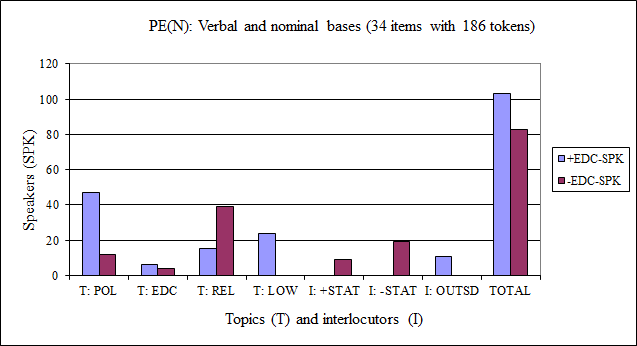
\includegraphics[scale=0.7]{./figures/Figure_3_3}
\begin{tikzpicture}
\begin{axis}[klugeaxis,title={\textscItal{pe(n)-}: Verbal and nominal bases (34 items with 186 tokens)}]
\addplot[klugedots]	coordinates {(1,47)(2,6)(3,15)(4,24)(5,0)(6,0)(7,11)(8,103)};
\addplot[klugelines] coordinates {(1,12)(2,4)(3,39)(4,0)(5,9)(6,19)(7,0)(8,83)};		
\legend{\textsc{+edc-spk},\textsc{-edc-spk}}
\end{axis}
\end{tikzpicture}
\caption[Token frequencies for {pe(n)-}prefixed lexemes with verbal and nominal bases by speakers, topics, and interlocutors]{Token frequencies for \textscItal{pe(n)-}prefixed lexemes with verbal and nominal bases by speakers, topics, and interlocutors}\label{Figure_3.3}
\end{figure}


The data given in \tabref{Table_3.13} and \figref{Figure_3.3} shows that for the 34 \textscItal{pe(n)-}prefixed lexemes, most tokens (167/186 – 90\%) can be explained in terms of speaker education levels, topics, and/or role-relations between the speakers and their interlocutors; this total includes 135/153 (88\%) tokens with verbal and 32/33 tokens (97\%) with nominal bases.


More than half of the tokens were produced by better-educated speakers (\textsc{+edc-spk}) (103/186 – 55\%), while less-educated speakers (\textsc{-edc-spk}) produced 83/186 tokens (45\%).



Two thirds of the 186 tokens (123/186 – 66\%) occurred during conversations about \textsc{high} topics, that is, political, educational or religious affairs (\textsc{pol}, \textsc{edc} and \textsc{rel}, respectively). This includes 68/103 tokens (66\%) produced by \textsc{+edc-spk} and 55/83 tokens (66\%) produced by \textsc{-edc-spk}. In addition, 11/186 tokens (6\%) occurred during conversations with an outsider, namely the author (\textsc{outsd}), all of them being \textsc{+edc-spk} tokens (11/103 – 11\%).



This leaves 52/186 tokens (28\%) that were produced when the interlocutors discussed \textsc{low} topics. This includes 24/103 \textsc{+edc-spk} tokens (23\%) and 28/83 \textsc{-edc-spk} tokens (34\%). The 28 \textsc{low} topic tokens produced by \textsc{-edc-spk} are distributed as follows. Nine tokens occurred during conversations with \textsc{+stat} Papuans (that is, 9/83 \textsc{-edc-spk} tokens – 11\%). The remaining 19 tokens (that is, 19/83 \textsc{-edc-spk} tokens – 23\%) occurred when \textsc{-edc-spk} discussed \textsc{low} topics with \textsc{-stat} Papuans, and therefore cannot be explained in terms of speaker education levels, topics, and/or role-relations. This total of 19 tokens refers to 10\% of all 186 \textscItal{pe(n)-}tokens, including 18/153 tokens (12\%) with verbal bases and 1/33 tokens (3\%) with nominal bases.\footnote{Concerning the 11 hapaxes (nine with verbal and two with nominal bases), the data suggests that seven are conditioned by the variables of speaker education levels, topics, and/or role-relations, and therefore are best explained as code-switches with \ili{Standard Indonesian}. This leaves only four hapaxes (with verbal bases) that cannot be accounted for in terms of language external factors and that are likely to result from a productive \isi{word-formation} process. For four hapaxes P=0.0376 as opposed to P=0.0591 for 11 hapaxes (N=186).}


\subsubsection[Summary and conclusions]{Summary and conclusions}\label{Para_3.1.4.5}

\largerpage
Prefix \textscItal{pe(n)-} is polyfunctional, in that it derives nouns from verbal and nominal bases. This polyfunctionality suggests that \isi{affixation} with \textscItal{pe(n)-} is a somewhat productive process (see language internal factor (\ref{List_3.1.c}) in §\ref{Para_3.1.1}, p. \pageref{List_3.1.c}).



Concerning \textscItal{pe(n)-}\isi{affixation} of verbal bases, three other observations support this conclusion: (1) the transparent form-function relationship between the derived nouns and their respective bases, (2) the large number of low frequency words and small number of high frequency words, and (3) the relative token frequencies with most bases having higher frequencies than the affixed lexemes. On the other hand, more than half of the derived lexemes were tentatively classified as SI-borrowings. These observations suggest that productivity of the \isi{affixation} process is rather limited.



As for \textscItal{pe(n)-}\isi{affixation} of nominal bases, two observations suggest that this is a productive process: (1) most of the derived lexemes are low frequency words, and (2) most bases have higher token frequencies than the affixed lexemes. On the other hand, almost all derived lexemes were tentatively classified as SI-borrowings. These findings suggest that \textscItal{pe(n)-}\isi{affixation} of nominal bases has limited productivity



As for the speech situations during which the derived nouns occurred, the vast majority of the attested tokens are conditioned by the variables of speaker education levels, topics, and/or role-relations. Hence, these items are best explained as code-switches with Indonesian.


\largerpage[2]
These findings suggest that in Papuan Malay \textscItal{pe(n)-} \isi{affixation} has, at best, margin\-al productivity.


\subsection[Prefix {\BER}- ‘\textsc{vblz}’]{Prefix \textscItal{ber-} ‘\textsc{vblz}’}\label{Para_3.1.5}

Prefix \textscItal{ber-} ‘\textsc{vblz}’ is typically attached to verbal bases, as in (\ref{Example_3.32}), or to nominal bases. Besides, the corpus also includes a few lexical items with \isi{numeral} and \isi{quantifier} bases. The prefixed lexemes have a verbal reading. As shown throughout this section, however, \isi{affixation} with \textscItal{ber-} ‘\textsc{vblz}’ is not used as a productive derivation device in Papuan Malay.

\ea
\label{Example_3.32}
\gll {\ldots} {waktu} {saya} {\bluebold{ber–buru}} {saya} {perlu} {makang} {pinang}\\ %
 { }  time  \textsc{1sg}  \textsc{vblz}–hunt  \textsc{1sg}  need  eat  betel.nut\\
\glt 
‘\ldots when I \bluebold{hunt} I need to chew betel nuts’ \textstyleExampleSource{[080919-004-NP.0011]}
\z



The corpus contains 62 derived verbs (602 tokens) prefixed with \textscItal{ber-}:\footnote{The 62 verbs include 25 hapaxes (P=0.0415); the 29 verbs with verbal bases include 11 hapaxes (P=0.0484); the 33 verbs with nominal, \isi{numeral}, or \isi{quantifier} bases include 14 hapaxes (P=0.0373).}



\begin{enumerate}
\item 
Verbs with verbal bases (29 items with 227 tokens)
\item 
Verbs with nominal, \isi{numeral}, or \isi{quantifier} bases (33 items with 375 tokens)

\end{enumerate}

The corpus also includes 16 formally complex words with non-compositional semantics, such as \textitbf{bertriak} ‘scream’, \textitbf{berjuang} ‘struggle’, or \textitbf{berlabu} ‘anchor’.



Before discussing \textscItal{ber-}\isi{affixation} of verbal bases in §\ref{Para_3.1.5.2} and of nominal, \isi{numeral}, and \isi{quantifier} bases in §\ref{Para_3.1.5.3}, the \isi{allomorphy} of \textscItal{ber-} is investigated in §\ref{Para_3.1.5.1}. Pertinent variables of the \isi{communicative event} that may impact the use of \textscItal{ber-} are explored in §\ref{Para_3.1.8}. The main findings on prefix \textscItal{ber-} are summarized and evaluated in §\ref{Para_3.1.5.4}.


\subsubsection[Allomorphy of ber-]{Allomorphy of \textscItal{ber-}}\label{Para_3.1.5.1}

Prefix \textscItal{ber-} has two allomorphs, \textitbf{ber}- and \textitbf{ba}-. The allomorphs are not governed by phonological processes.

\largerpage

\begin{table} 
\caption{Realizations of allomorph \textitbf{ber}-}\label{Table_3.14}

\begin{tabular}{lll}
\lsptoprule

 \multicolumn{1}{c}{\textitbf{ber}\textsc{-}base} & \multicolumn{1}{c}{Orthogr.} &  \multicolumn{1}{c}{Gloss}\\

\midrule
/\textstyleChCharisSIL{bɛr}–\textstyleChCharisSIL{dʒuaŋ}/ & \textitbf{berjuang} & ‘struggle (for)’\\

/\textstyleChCharisSIL{br}–\textstyleChCharisSIL{aŋkat}/ & \textitbf{brangkat} & ‘leave’\\

/\textstyleChCharisSIL{bl}–\textstyleChCharisSIL{adʒar}/ & \textitbf{blajar} & ‘study’\\

/\textstyleChCharisSIL{bɛ}–\textstyleChCharisSIL{kɛrdʒa}/ & \textitbf{bekerja} & ‘work’\\

/\textstyleChCharisSIL{bɛ}–\textstyleChCharisSIL{brapa}/ & \textitbf{bebrapa} & ‘be several’\\

\lspbottomrule
\end{tabular}
\end{table}

The form \textitbf{ber}-, in turn, has four realizations that are effected by morphologically conditioned phonological rules. More specifically, the four allomorphs are conditioned by the word-initial segment of the base word, as illustrated in \tabref{Table_3.14}: /\textstyleChCharisSIL{bɛr-}/, /\textstyleChCharisSIL{br-}/, /\textstyleChCharisSIL{bl-}/, and /\textstyleChCharisSIL{bɛ-}/. The prefix is typically realized as /\textstyleChCharisSIL{bɛr-}/. With an onset vowel, however, \textitbf{ber}- is very commonly realized as /br\textstyleChCharisSIL{-}/. When prefixed to \textitbf{ajar} ‘teach’ the prefix is realized as /\textstyleChCharisSIL{bl-}/, while it is realized as /\textstyleChCharisSIL{bɛ-}/ when affixed to \textitbf{kerja} ‘work’ or \textitbf{brapa} ‘several’.

Allomorph \textitbf{ba}- occurs much less frequently. Attested are only the 15 items listed in \tabref{Table_3.15} with a total of 37 tokens. Some of these items are alternatively realized with allomorph \textitbf{ber}-. Therefore, for each item the token frequencies for \textitbf{ba}- and for \textitbf{ber}- are given. If in a greater number of tokens the prefix is realized with /\textstyleChCharisSIL{ba-}/ rather than with /\textstyleChCharisSIL{bɛr-}/, then its orthographic representation is \textitbf{ba}- as in \textitbf{bakalay} ‘fight’. If both realizations have the same token frequencies, then the orthographic representation follows its realization in the recorded texts, as in \textitbf{bergaya} ‘put on airs’.

\begin{table}[b]
\caption{ Realizations of allomorph \textitbf{ba}-}\label{Table_3.15}


\begin{tabular}{lllrr}
\lsptoprule
 \multicolumn{1}{c}{\textitbf{ba-}base} & \multicolumn{1}{c}{Orthogr.} & \multicolumn{1}{c}{Gloss} & \multicolumn{1}{c}{\textitbf{ba-} \#} &  \multicolumn{1}{c}{\textitbf{ber-} \#}\\
\midrule

/\textstyleChCharisSIL{ba}–\textstyleChCharisSIL{kalaj}/ & \textitbf{bakalay} & ‘fight’ &  19 &  0\\

/\textstyleChCharisSIL{ba}–\textstyleChCharisSIL{taria}/ & \textitbf{bertriak}\footnote{The root is realized as /\textstyleChCharisSILviiivpt{triak}/ when speakers employ allomorph \textitbf{ber}-, whereas it is realized as /\textstyleChCharisSILviiivpt{taria}/ when speakers use allomorph \textitbf{ba}-.}
 & ‘scream’ &  3 &  18\\

/\textstyleChCharisSIL{ba}–\textstyleChCharisSIL{biŋuŋ}/ & \textitbf{babingung} & ‘be confused’ &  2 &  0\\

/\textstyleChCharisSIL{ba}–\textstyleChCharisSIL{diam}/ & \textitbf{badiam} & ‘be quiet’ &  2 &  0\\

/\textstyleChCharisSIL{ba}–\textstyleChCharisSIL{diri}/ & \textitbf{berdiri} & ‘stand’ &  1 &  54\\

/\textstyleChCharisSIL{ba}–\textstyleChCharisSIL{dara}/ & \textitbf{berdara} & ‘bloody’ &  1 &  1\\

/\textstyleChCharisSIL{ba}–duri/ & \textitbf{berduri} & ‘be thorny’ &  1 &  1\\

/\textstyleChCharisSIL{ba}–\textstyleChCharisSIL{gaja}/ & \textitbf{bergaya} & ‘put on airs’ &  1 &  1\\

/\textstyleChCharisSIL{ba}–gisi/ & \textitbf{bergisi} & ‘be nutritious’ &  1 &  1\\

/\textstyleChCharisSIL{ba}–jalang/ & \textitbf{berjalang} & ‘walk’ &  1 &  1\\

/\textstyleChCharisSIL{ba}–ribut/ & \textitbf{beribut} & ‘be noisy’ &  1 &  1\\

/\textstyleChCharisSIL{ba}–\textstyleChCharisSIL{gigit}/ & \textitbf{bagigit} & ‘bite’ &  1 &  0\\

/\textstyleChCharisSIL{ba}–\textstyleChCharisSIL{kumis}/ & \textitbf{bakumis} & ‘have a beard’ &  1 &  0\\

/\textstyleChCharisSIL{ba}–\textstyleChCharisSIL{isi}/ & \textitbf{baisi} & ‘be muscular’ &  1 &  0\\

/\textstyleChCharisSIL{ba}–\textstyleChCharisSIL{mɛkap}/ & \textitbf{bamekap} & ‘wear make-up’ &  1 &  0\\

\lspbottomrule
\end{tabular}
\end{table}

In realizing prefix \textscItal{ber-} most commonly as allomorph \textitbf{ber}- rather than as \textitbf{ba}-, Papuan Malay again contrasts with other \ili{eastern Malay varieties} such as \ili{Ambon Malay} \citep[95]{vanMinde.1997}, \ili{Banda Malay} \citep[249]{Paauw.2009}, \ili{Kupang Malay} \citep[46]{Steinhauer.1983}, \ili{Manado Malay} \citep[18]{Stoel.2005}, and North Moluccan / \ili{Ternate Malay} (\citealt[18]{Taylor.1983}; \citealt[4]{Voorhoeve.1983}; \citealt[125]{Litamahuputty.2012}). In these varieties the prefix is always realized as \textitbf{ba}-. Instead, the items prefixed with \textscItal{ber-} have more resemblance with the corresponding Indonesian items where the prefix is realized as \textitbf{ber}-. In addition, in \ili{Larantuka Malay} the prefix is also realized as \textitbf{bə}\textbf{(}\textitbf{r}\textbf{)}- {\citep[253]{Paauw.2009}}. Again this difference between Papuan Malay and the other \ili{eastern Malay varieties} points to the distinct histories of both, discussed in §\ref{Para_1.8}.


\subsubsection[Prefixed items derived from verbal bases]{Prefixed items derived from verbal bases}\label{Para_3.1.5.2}

The corpus includes 29 \textscItal{ber-}prefixed lexemes (with 227 tokens) with verbal bases, as listed in Table  \ref{Table_3.16a} and Table \ref{Table_3.16b}. Of the 29 lexemes, 11 have \isi{monovalent} bases such as stative \textitbf{diam} ‘be quiet’ or dynamic \textitbf{jalang} ‘walk’. The remaining 18 items have \isi{bivalent} bases. Of these 18 prefixed lexemes, five have monotransitive as well as intransitive uses, while 11 lexemes have intransitive uses only. These 16 lexemes have the same semantics as their \isi{bivalent} bases, as shown in (\ref{Example_3.33}) to (\ref{Example_3.43}). For the remaining two prefixed lexemes the semantics are distinct from those of their bases, as shown in (\ref{Example_3.44}) to (\ref{Example_3.50}). One of them has monotransitive as well as intransitive uses, while the other one has intransitive uses only.



Almost all of the derived lexemes are low frequency words (27 lexemes, attested with less than 20 tokens). Moreover, the token frequencies for the respective bases are (much) higher for most of the derived words (22 lexemes). This is due to the fact that the affixed lexemes and the bases have the same semantics and that, overall, speakers tend to use the bases rather than the prefixed forms, as shown in (\ref{Example_3.33}) to (\ref{Example_3.43}). Also, most of the 29 prefixed lexemes (24 items) were tentatively classified as borrowings from \ili{Standard Indonesian} (SI-borrowings) (for details see language internal factor (\ref{List_3.1.f}) in §\ref{Para_3.1.1}, p. \pageref{List_3.1.f}); in Table  \ref{Table_3.16a} and Table \ref{Table_3.16b} these items are underlined.

\begin{table}
\caption[Affixation with {ber-} of verbal bases]{Affixation with \textscItal{ber-} of verbal bases}\label{Table_3.16a}

\begin{tabularx}{\textwidth}{lllrr}
\lsptoprule

\multicolumn{1}{c}{BW} & \multicolumn{1}{c}{Item} & \multicolumn{1}{c}{Gloss} & \multicolumn{1}{c}{\textscItal{ber-} \#} &  \multicolumn{1}{c}{BW \#}\\
\midrule
\multicolumn{5}{l}{Monovalent bases: Bases and prefixed lexemes with same semantics}\\
\midrule
 \textitbf{tobat} & {\textitbfUndl{bertobat}} & ‘repent’ &  8 &  1\\

 \textitbf{beda} & {\textitbfUndl{berbeda}} & ‘be different’ &  7 &  34\\

 \textitbf{tanggung-jawap} & {\textitbfUndl{bertanggung-jawap}} & ‘be responsible’ &  5 &  6\\

 \textitbf{bahaya} & {\textitbfUndl{berbahaya}} & ‘be dangerous’ &  3 &  3\\

 \textitbf{diam} & {\textitbfUndl{badiam}} & ‘be quiet’ &  2 &  60\\

 \textitbf{bingung} & {\textitbfUndl{berbingung}} & ‘be confused’ &  2 &  30\\

 \textitbf{jalang} & {\textitbfUndl{berjalang}} & ‘walk’ &  1 &  480\\

 \textitbf{ibada} & {\textitbfUndl{beribada}} & ‘worship’ &  1 &  11\\

 \textitbf{sandar} & {\textitbfUndl{bersandar}} & ‘lean’ &  1 &  6\\

 \textitbf{hati{\Tilde}hati} & {\textitbfUndl{berhati{\Tilde}hati}} & ‘be careful’ &  1 &  5\\

 \textitbf{pisa} & {\textitbfUndl{berpisa}} & ‘be separate’ &  1 &  4\\
\midrule
\multicolumn{5}{l}{Bivalent bases: Bases and prefixed lexemes with same semantics}\\
\midrule
% \multicolumn{5}{l}{  Prefixed lexemes: Monotransitive and intransitive uses}\\

 \textitbf{buru} & {\textitbf{berburu}} & ‘hunt’ & 10 &  5\\

 \textitbf{buat} & {\textitbfUndl{berbuat}} & ‘make’ & 7 &  100\\

 \textitbf{pikir} & {\textitbfUndl{berpikir}} & ‘think’ & 8 &  102\\

 \textitbf{harap} & {\textitbfUndl{berharap}} & ‘hope’ &  1 &  8\\

 \textitbf{ribut} & {\textitbf{bribut}} & ‘trouble’ &  1 &  5\\

\tablevspace
% \multicolumn{5}{l}{  Prefixed lexemes: Monotransitive uses}\\
 \textitbf{bicara} & \textitbfUndl{berbicara} & {‘speak’} & 7 &  333\\

 \textitbf{kerja} & \textitbfUndl{bekerja} & {‘work’} & 5 &  191\\

 \textitbf{tahang} & \textitbfUndl{bertahang} & {‘hold (out/back)’} & 5 &  48\\

 \textitbf{uba} & \textitbf{bruba} & {‘change’} & 5 &  9\\

 \textitbf{gabung} & \textitbfUndl{bergabung} & {‘join’} & 4 &  3\\

 \textitbf{maing} & \textitbfUndl{bermaing} & {‘play’} &  3 &  113\\

 \textitbf{tindak} & \textitbfUndl{bertindak} & {‘act’} &  2 &  1\\

 \textitbf{ikut} & \textitbfUndl{brikut} & {‘follow’} &  1 &  259\\

 \textitbf{kumpul} & \textitbfUndl{berkumpul} & {‘gather’} &  1 &  16\\

 \textitbf{bentuk} & \textitbfUndl{berbentuk} & {‘form’} &  1 &  12\\

 \textitbf{gigit} & \textitbfUndl{bergigit} & {‘bite’} &  1 &  10\\
\lspbottomrule
\end{tabularx}
\end{table}
\begin{table}
\caption[Affixation with {ber-} of verbal bases continued]{Affixation with \textscItal{ber-} of verbal bases continued}\label{Table_3.16b}

\begin{tabularx}{\textwidth}{lllrr}
\lsptoprule

\multicolumn{1}{c}{BW} & \multicolumn{1}{c}{Item} & \multicolumn{1}{c}{Gloss} & \multicolumn{1}{c}{\textscItal{ber-} \#} &  \multicolumn{1}{c}{BW \#}\\
\midrule
\multicolumn{5}{l}{Bivalent bases: Bases and prefixed lexemes with distinct semantics}\\
\midrule
\multicolumn{5}{l}{Prefixed lexeme: Monotransitive and intransitive uses}\\

 \textitbf{ajar} (‘teach’) & {\textitbf{blajar}\hspace{2.3cm}} & ‘study’\hspace{1cm} & 51 &  41\\
\\
% \todo[inline]{check spacing}\\
\multicolumn{5}{l}{Prefixed lexeme: Monotransitive uses}\\

 \textitbf{angkat} (‘lift’) & {\textitbf{brangkat}} & ‘leave’ & 82 &  81\\

\lspbottomrule
\end{tabularx}
\end{table}

Affixation with \textscItal{ber-} of verbal bases derives lexemes that typically have the same semantics as their respective bases, with \textscItal{ber-} being glossed as ‘\textsc{vblz}’ (``verbalizer''). This applies to \textscItal{ber-}prefixed lexemes with \isi{monovalent} and with \isi{bivalent} bases.


The fact that \isi{monovalent} bases derive \textscItal{ber-}prefixed lexemes with the same semantics is illustrated with stative \textitbf{bingung} ‘be confused’ and prefixed \textitbf{berbingung} ‘be confused’ in (\ref{Example_3.33}) and (\ref{Example_3.34}), and with dynamic \textitbf{ibada} ‘worship’ and prefixed \textitbf{beribada} ‘worship’ in (\ref{Example_3.35}) and (\ref{Example_3.36}), respectively.



\begin{styleExampleTitle}
{Prefix \textscItal{ber-}: Semantics of verbal bases and derived lexemes}
\end{styleExampleTitle}

\ea
\label{Example_3.33}
\gll {memang} {sa} {punya} {ade} {sa} {juga} {\bluebold{bingung}} {dengang} {dia}\\ %
 indeed  \textsc{1sg}  \textsc{poss}  ySb  \textsc{1sg}  also  be.confused  with  \textsc{3sg}\\
\glt 
‘indeed (he was) my younger cousin, I’m also \bluebold{confused} about him’ \textstyleExampleSource{[080918-001-CvNP.0014]}
\z

 

\ea
\label{Example_3.34}
\gll {{nanti}} {di} {skola} {baru} {kamu} {\bluebold{ba–bingung}} {dengang}\\ %
 {very.soon}  at  school  and.then  \textsc{2pl}  \textsc{vblz}–be.confused  with\\

 bahasa  {Inggris}\\

 language  {English}\\

\glt 
[Addressing lazy students:] ‘later in school, then you’ll be \bluebold{confused} about English’ \textstyleExampleSource{[081115-001a-Cv.0151]}
\z

\ea
\label{Example_3.35}
\gll {orang} {jalang} {itu} {mo} {pergi} {\bluebold{ibada}}\\ %
 person  walk  \textsc{d.dist}  want  go  worship\\
\glt 
[About a youth retreat:] ‘people doing that traveling want to go (and) \bluebold{worship}’ \textstyleExampleSource{[081006-016-Cv.0017]}
\z

\ea
\label{Example_3.36}
\gll {{nanti}} {{kita}} {\bluebold{ber–ibada}} {selesay} {malam} {ka}\\ %
 {very.soon}  {\textsc{1pl}}  \textsc{vblz}–worship  finish  night  maybe\\
\gll baru  {sa}  {pergi}\\
 and.then  {\textsc{1sg}}  {go}\\
\glt 
‘later, after we have \bluebold{worshipped}, maybe in the evening, and then I’ll go (there)’ \textstyleExampleSource{[080918-001-CvNP.0016]}\footnotetext{The original recording says \textitbf{kita i beribada selesay}. Most likely the speaker wanted to say \textitbf{kita ibada selesay} ‘after we have worshipped’ but cut himself off to replace \textitbf{ibada} ‘worship’ with \textitbf{beribada} ‘worship’.}
\z

Bivalent bases also derive \textscItal{ber-}prefixed lexemes that have the same semantics as their bases, as shown in (\ref{Example_3.37}) to (\ref{Example_3.43}). As discussed in §\ref{Para_11.1.2}, \isi{bivalent} verbs have not only monotransitive but also intransitive uses. The same applies to some of the \textscItal{ber-}prefixed lexemes, as illustrated in (\ref{Example_3.37}) to (\ref{Example_3.40}).



\begin{styleExampleTitle}
{Prefix \textscItal{ber-}: Same semantics of verbal bases and derived lexemes}
\end{styleExampleTitle}

\ea
\label{Example_3.37}
\gll {jadi} {kitorang} {bingung} {\bluebold{pikir}} {itu} {pen–jaga} {kubur\bluebold{–}ang}\\ %
 so  \textsc{1pl}  be.confused  think  \textsc{d.dist}  \textsc{ag}–guard  bury–\textsc{pat}\\
\glt 
‘so we’re confused to \bluebold{think (about)}, what’s-its-name, a guard (for) the grave’ \textstyleExampleSource{[080923-007-Cv.0024]}
\z

\ea
\label{Example_3.38}
\gll   {\ldots}  tapi  ana{\Tilde}ana  ni  dong  tida  taw  \bluebold{ber–pikir}  itu\\
  { }  but  \textsc{rdp}{\Tilde}child  \textsc{d.prox}  \textsc{3pl}  \textsc{neg}  know  \textsc{vblz}–think  \textsc{d.dist}\\
\glt 
[About impolite teenagers:] ‘{\ldots} but these kids they don’t know (how) to \bluebold{think (about)} those (feelings of mine)’ \textstyleExampleSource{[081115-001b-Cv.0037]}
\z

\ea
\label{Example_3.39}
\gll {skarang}  orang  su  tra  \bluebold{pikir}  tentang\\
 {now}  person  already  \textsc{neg}  think  about\\
\gll hal  {ke–benar–ang}\\
 thing  {\textsc{nmlz}–be.true–\textsc{nmlz}}\\
\glt 
‘nowadays, the people already don’t \bluebold{think} about things (related to) truth’ \textstyleExampleSource{[081006-032-Cv.0016]}
\z

\ea
\label{Example_3.40}
\gll {\ldots} {karna} {dia} {\bluebold{ber–pikir}} {tentang} {dia} {punya} {badang}\\ %
 { }  because  \textsc{3sg}  \textsc{vblz}–think  about  \textsc{3sg}  \textsc{poss}  body\\
\glt 
‘[she doesn’t think about serving my or her guests] because she \bluebold{thinks} about her body’ \textstyleExampleSource{[081006-032-Cv.0062]}
\z


Most \textscItal{ber-}prefixed lexemes with \isi{bivalent} bases, however, have intransitive uses only, while their bases can be used mono- or intransitively. This is illustrated with \textitbf{bicara} ‘speak’ and \textitbf{berbicara} ‘speak’ in (\ref{Example_3.41}) to (\ref{Example_3.43}).



\begin{styleExampleTitle}
Prefix \textscItal{ber-}: Semantics and distribution of verbal bases and derived lexemes
\end{styleExampleTitle}

\ea
\label{Example_3.41}
\gll {baru} {de} {\bluebold{bicara}} {sa} {deng} {bahasa} {Inggris}\\ %
 and.then  \textsc{3sg}  speak  \textsc{1sg}  with  language  English\\

\glt 
‘and then she \bluebold{talked (to)} me in English’ \textstyleExampleSource{[081115-001a-Cv.0229]}
\z

\ea
\label{Example_3.42}
\gll  de  \bluebold{bicara}  trus\\
 \textsc{3sg}  speak  be.continuous\\
\glt 
‘he kept \bluebold{talking}’ \textstyleExampleSource{[080922-010a-CvNF.0145]}
\z
\ea
\label{Example_3.43}
\gll {baru} {nanti} {\bluebold{ber–bicara}} {untuk} {nika}\\ %
 and.then  very.soon  \textsc{vblz}–speak  for  marry.officially\\
\glt 
[About wedding customs:] ‘and then very soon (they’ll) \bluebold{talk} about marrying’ \textstyleExampleSource{[081110-006-CvEx.0050]}
\z


The corpus includes only two \textscItal{ber-}prefixed lexemes that have distinct semantics vis-à-vis their \isi{bivalent} bases, namely \textitbf{ajar} ‘teach’ and prefixed \textitbf{blajar} ‘study’, and \textitbf{angkat} ‘lift’ and prefixed \textitbf{brangkat} ‘leave’ as shown in (\ref{Example_3.44}) to (\ref{Example_3.50}). Both \textitbf{ajar} ‘teach’ and \textitbf{blajar} ‘study’ are used monotransitively as in (\ref{Example_3.44}) and (\ref{Example_3.45}), as well as intransitively as in (\ref{Example_3.46}) and (\ref{Example_3.47}), respectively; in each case both lexemes maintain their distinct semantics.



\begin{styleExampleTitle}
{Prefix \textscItal{ber-}: Distinct semantics and same distribution of verbal bases and derived lexemes}
\end{styleExampleTitle}

\ea
\label{Example_3.44}
\gll {de} {\bluebold{ajar}} {dorang} {tu} {untuk} {baik}\\ %
 \textsc{3sg}  teach  \textsc{3pl}  \textsc{d.dist}  for  be.good\\
\glt 
‘she \bluebold{teaches} them there for (their own) good’ \textstyleExampleSource{[081115-001a-Cv.0216]}
\z

\ea
\label{Example_3.45}
\gll {Ise} {de} {\ldots} {{ikut}} {bahasa} {Inggris} {\bluebold{bl–ajar}} {kursus,}\\ %
 Ise  \textsc{3sg} {}   {follow}  language  English  \textsc{vblz}–teach  course\\
\gll {bahasa}  {Inggris}  {dulu}\\
 {language}  {English}  {first}\\
\glt 
‘Ise will participate in an English (course), (she’ll) \bluebold{study} a course, an English language course first’ \textstyleExampleSource{[081025-003-Cv.0223]}
\z

\ea
\label{Example_3.46}
\gll {de} {suda} {\bluebold{ajar}} {bagus} {tiap} {sore} {itu}\\ %
 \textsc{3sg}  already  teach  be.good  every  afternoon  \textsc{d.dist}\\
\glt 
‘she’s already been \bluebold{teaching} well, each and every afternoon’ \textstyleExampleSource{[081115-001a-Cv.0126]}
\z
\ea
\label{Example_3.47}
\gll {dong} {tida} {\bluebold{bl–ajar}} {baik}\\ %
 \textsc{3pl}  \textsc{neg}  \textsc{vblz}–teach  be.good\\

\glt 
‘they don’t \bluebold{study} well’ \textstyleExampleSource{[081115-001b-Cv.0067]}
\z


Bivalent \textitbf{angkat} ‘lift’ and prefixed \textitbf{brangkat} ‘leave’ also have distinct semantics. In addition, they also have a distinct distribution. The base \textitbf{angkat} ‘lift’ is used monotransitively, as well as intransitively, as in (\ref{Example_3.48}) and (\ref{Example_3.49}), respectively. By contrast, \textitbf{brangkat} ‘leave’ is always used intransitively, as in (\ref{Example_3.50}).



\begin{styleExampleTitle}
{Prefix \textscItal{ber-}: Distinct semantics and distinct distribution of \isi{verbal base} and derived lexeme}
\end{styleExampleTitle}
\ea
\label{Example_3.48}
\gll {bapa} {de} {\bluebold{angkat}} {rotang} {besar}\\ %
 father  \textsc{3sg}  lift  rattan  be.big\\
\glt 
‘father \bluebold{picked up} a big rattan (stick)’ \textstyleExampleSource{[080921-004a-CvNP.0084]}
\z
\ea
\label{Example_3.49}
\gll {sa} {sendiri} {tra} {bisa} {\bluebold{angkat}}\\ %
 \textsc{1sg}  be.alone  \textsc{neg}  be.able  lift\\
\glt 
‘[the pig was very big,] I alone could not \bluebold{transport} (it)’ \textstyleExampleSource{[080919-003-NP.0008]}
\z
\ea
\label{Example_3.50}
\gll {skarang} {de} {mo} {\bluebold{br–angkat}}\\ %
 now  \textsc{3sg}  want  \textsc{vblz}–lift\\
\glt 
‘then he wanted to \bluebold{leave}’ \textstyleExampleSource{[080919-007-CvNP.0023]}
\z


In summary, with the exception of the last two lexemes, \textscItal{ber-}prefixed verbs have the same semantics as their respective bases. This suggests that in Papuan Malay \isi{affixation} of verbal bases with prefix \textscItal{ber-} is not a productive process. Instead, the attested prefixed lexemes and their bases are taken as pairs of words from two different speech varieties: the unaffixed items are native Papuan Malay lexemes whereas the corresponding affixed items are SI-borrowings.



Given these properties, Papuan Malay \textscItal{ber-} contrasts with the corresponding prefix in other Malay varieties. In most \ili{eastern Malay varieties}, the corresponding prefix \textitbf{ba}- forms verbs with a variety of meanings. The most common ones are durative and reflexive meanings, which are reported for \ili{Ambon Malay} \citep[96–98]{vanMinde.1997}, \ili{Banda Malay} \citep[249--250]{Paauw.2009},\footnote{For \ili{Banda Malay}, \citet[249]{Paauw.2009} reports that \textitbf{ba}- does not form verbs with reflexive meanings.} \ili{Manado Malay} \citep[18–22]{Stoel.2005}, and North Moluccan / \ili{Ternate Malay} (\citealt[18]{Taylor.1983}; \citealt[125–127]{Litamahuputty.2012}). In \ili{Kupang Malay} \citep[46–49]{Steinhauer.1983} and \ili{Larantuka Malay} \citep[249–254-255]{Paauw.2009}, the prefix typically signals durative and reciprocal meanings. In \ili{Standard Indonesian}, the main function of the corresponding prefix \textitbf{ber-} is to create \isi{monovalent} verbs (\citealt[131]{Englebretson.2003}; \citeyear*[96]{Englebretson.2007}). When attached to verbal bases, the prefix indicates “that the subject of the utterance is the patient, that is, the experiencer of the action” \citep[134–138]{Mintz.1994}.


\subsubsection[Prefixed items derived from nominal, {numeral}, or {quantifier} bases]{Prefixed items derived from nominal, {numeral}, or {quantifier} bases}\label{Para_3.1.5.3}

The corpus contains 33 \textscItal{ber-}prefixed lexemes (with 375 tokens), as listed in  \tabref{Table_3.17a} and \tabref{Table_3.17b}: 30 lexemes with nominal bases (362 tokens), two lexemes with \isi{numeral} bases (7 tokens), and one lexeme with a \isi{quantifier} base (6 tokens).



Most of the derived lexemes are low frequency words (29 lexemes, attested with less than 20 tokens). Besides, the token frequencies for the respective bases are (much) higher for most of the derived words (21 lexemes). This is due to the fact that Papuan Malay speakers typically use alternative analytical constructions to convey the meanings of the prefixed lexemes, as shown below in (\ref{Example_3.51}) to (\ref{Example_3.56}). Further, most of the 33 items (25 items) were tentatively classified as SI-borrowings (for details see language internal factor (\ref{List_3.1.f}) in §\ref{Para_3.1.1}, p. \pageref{List_3.1.f}); in \tabref{Table_3.17a} and \tabref{Table_3.17b} these items are underlined.

\begin{table}[b]
\caption[Affixation with {ber-} of nominal, \isi{numeral}, and \isi{quantifier} bases]{Affixation with \textscItal{ber-} of nominal, \isi{numeral}, and \isi{quantifier} bases}\label{Table_3.17a}
\begin{tabularx}{\textwidth}{llll>{\raggedleft}Xr}
\lsptoprule
 \multicolumn{1}{c}{BW} & \multicolumn{1}{c}{Gloss} & \multicolumn{1}{c}{Item} & \multicolumn{1}{c}{Gloss} & \multicolumn{1}{c}{\textscItal{ber-} \#} &  \multicolumn{1}{c}{BW \#}\\
\midrule
\multicolumn{6}{l}{Nominal bases}\\
\midrule
\textitbf{doa} & ‘prayer’ & \textitbf{berdoa} & ‘pray’ &  136 &  20\\

\textitbf{arti} & ‘meaning’ & \textitbf{brarti} & ‘mean’ &  89 &  7\\

\textitbf{diri} & ‘self’ & \textitbf{berdiri} & ‘stand’ &  55 &  14\\

\textitbf{usaha} & ‘effort’ & \textitbf{berusaha} & ‘attempt’ &  25 &  2\\

\textitbf{dosa} & ‘sin’ & \textitbf{berdosa} & ‘sin’ &  6 &  4\\

\textitbf{saksi} & ‘witness’ & \textitbfUndl{bersaksi} & ‘testify’ &  6 &  2\\

\textitbf{hasil} & ‘result’ & \textitbf{berhasil} & ‘succeed’ &  6 &  13\\

\textitbf{kwasa} & ‘power’ & \textitbfUndl{berkwasa} & ‘be powerful’ &  4 &  25\\

\textitbf{hak} & ‘right’ & \textitbfUndl{berhak} & ‘have right’ &  4 &  15\\

\textitbf{sodara} & ‘sibling’ & \textitbfUndl{bersodara} & ‘be siblings’ &  3 &  127\\

\textitbf{kebung} & ‘garden’ & \textitbfUndl{berkebung} & ‘do farming’ &  3 &  61\\

\textitbf{ade-kaka} & ‘siblings’ & \textitbfUndl{brade-kaka} & ‘be siblings’ &  2 &  26\\

\textitbf{malam} & ‘night’ & \textitbfUndl{bermalam} & ‘overnight’ &  2 &  191\\

\textitbf{bahasa} & ‘language’ & \textitbfUndl{berbahasa} & ‘speak’ &  2 &  136\\

\textitbf{temang} & ‘friend’ & \textitbfUndl{bertemang} & ‘be friends’ &  2 &  85\\

\textitbf{kluarga} & ‘family’ & \textitbfUndl{berkluarga} & ‘have family’ &  2 &  49\\

\textitbf{gaya} & ‘manner’ & \textitbf{bergaya} & ‘put on airs’ &  2 &  7\\

\textitbf{ana} & ‘child’ & \textitbf{brana} & ‘give birth’ &  1 &  739\\

\textitbf{bua} & ‘fruit’ & \textitbfUndl{berbua} & ‘have fruit’ &  1 &  38\\

\textitbf{dara} & ‘blood’ & \textitbfUndl{berdara} & ‘bleed’ &  1 &  27\\

\textitbf{sifat} & ‘characteristic’ & \textitbfUndl{bersifat} & ‘have characteristics of’ &  1 &  18\\

\textitbf{duri} & ‘thorn’ & \textitbfUndl{berduri} & ‘have thorns’ &  1 &  8\\

\textitbf{harga} & ‘value’ & \textitbfUndl{berharga} & ‘be valuable’ &  1 &  4\\

\textitbf{syukur} & ‘thanks’ & \textitbfUndl{bersyukur} & ‘give thanks’ &  1 &  2\\

\textitbf{fungsi} & ‘function’ & \textitbfUndl{berfungsi} & ‘function’ &  1 &  1\\

\textitbf{gisi} & ‘nutrient’ & \textitbfUndl{bergisi} & ‘be nutritious’ &  1 &  1\\

\textitbf{isi} & ‘content’ & \textitbfUndl{baisi} & ‘be muscular’ &  1 &  1\\
\lspbottomrule
\end{tabularx}
\end{table}
\begin{table}

\caption[Affixation with {ber-} of nominal, \isi{numeral}, and \isi{quantifier} bases continued]{Affixation with \textscItal{ber-} of nominal, \isi{numeral}, and \isi{quantifier} bases continued}\label{Table_3.17b}
{\setlength{\tabcolsep}{3pt}
\begin{tabularx}{\textwidth}{llllrr}
\lsptoprule

 BW & Gloss & Item & Gloss & \textscItal{ber-} \#\hspace{2mm} &  BW \#\\
\midrule

\textitbf{komunikasi} & ‘communica\-tion’ & \textitbfUndl{berkomuni\-}\textitbfUndl{kasi} & ‘communicate’ &  1 &  1\\

\textitbf{kumis} & ‘beard’ & \textitbfUndl{bakumis} & ‘have a beard’ &  1 &  1\\

\textitbf{mekap} & ‘make-up’ & \textitbfUndl{bamekap} & ‘wear make-up’ &  1 &  1\\
\midrule
\multicolumn{6}{l}{Numeral bases}\\
\midrule
\textitbf{satu} & ‘one’ & \textitbfUndl{bersatu} & ‘be one’ &  6 &  516\\

\textitbf{empat} & ‘four’ & \textitbfUndl{berempat} & ‘be four’ &  1 &  66\\
\midrule
\multicolumn{6}{l}{Quantifier base}\\
\midrule
\textitbf{brapa} & ‘several’ & \textitbfUndl{bebrapa} & ‘be several’ &  6 &  109\\

\lspbottomrule
\end{tabularx}
}
\end{table}

\newpage 
Affixation with \textscItal{ber-} derives \isi{monovalent} verbs with the general meaning of ‘be/have/ do \textsc{base}’. Examples are \textitbf{brarti} ‘have the meaning of’ or ‘mean’, \textitbf{berdoa} ‘do prayer’ or ‘pray’, \textitbf{bersatu} ‘be one’, or \textitbf{bebrapa} ‘be several’. The \isi{monovalent} \isi{verb} \textitbf{berdiri} ‘stand’ is an exception. Historically related to the \isi{noun} \textitbf{diri} ‘self’, it does not have a transparent form-function relationship to its base. The transparent form-function relationship between the remaining 32 items and their bases suggests that these lexemes are the result of a productive \isi{affixation} process. Two observations are made, however.


First, the data indicates that Papuan Malay speakers prefer to employ analytical constructions to express the meanings conveyed by the prefixed items, as illustrated in (\ref{Example_3.51}) to (\ref{Example_3.56}). To communicate ‘have \textsc{base}’, speakers typically use the existential \isi{verb} \textitbf{ada} ‘exist’ rather than the prefixed form, as shown in (\ref{Example_3.51}) with \textitbf{ada duri} versus \textitbf{berduri} ‘have thorns’.

\ea
\label{Example_3.51}
\gll {{ada}} {{\ldots}} {dua} {{macang}} {{jenis}} {{ada}} {{yang}} {{\bluebold{ber}\bluebold{–}\bluebold{duri}}} {ada} {yang}\\ %
 {exist}  {}  two  {variety}  {kind}  {exist}  {\textsc{rel}}  {\textsc{vblz}–thorn}  exist  \textsc{rel}\\
\\
\gll tida  {\ldots}  {kang}  {ada}  {sagu}  {yang}  {tida}  \bluebold{ada}  {\bluebold{duri}}\\
 \textsc{neg}  {}  {you.know}  {exist}  {sago}  {\textsc{rel}}  {\textsc{neg}}  exist  {thorn}\\

\glt 
‘there are {\ldots} two kinds (of sago palms), ones that \bluebold{have thorns} and ones that don’t (have thorns) {\ldots} you know (there are) sago (palms) that don’t \bluebold{have thorns}’ \textstyleExampleSource{[081014-006-CvPr.0007/0009]}
\z


To express ‘be \textsc{base}’, speakers use a nominal predicate such as \textitbf{ade-kaka} ‘siblings’ in (\ref{Example_3.52}), rather than the respective prefixed form \textitbf{brade-kaka} ‘be siblings’ as in (\ref{Example_3.53}).

\ea
\label{Example_3.52}
\glll {jadi} {saya} {dengang} {dia} \bluebold{ade-kaka} {sunggu}\\ %
 {} {} {} {} {ySb-oSb}\\
 so  \textsc{1sg}  with  \textsc{3sg}  siblings  be.true\\
\glt 
‘so I and she \bluebold{are} full \bluebold{siblings}’ \textstyleExampleSource{[080927-009-CvNP.0044]}
\z

\ea
\label{Example_3.53}
\gll {jadi} {saya} {dengang} {kaka} {Nofita} {masi} {\bluebold{br}\bluebold{–}\bluebold{ade-kaka}}\\ %
 so  \textsc{1sg}  with  oSb  Nofita  still  \textsc{vblz}–siblings\\
\glt 
‘so I and older sister Nofita \bluebold{are} still \bluebold{siblings}’ \textstyleExampleSource{[080927-007-CvNP.0022]}
\z


To communicate ‘do \textsc{base}’, speakers typically employ alternative verbs. They tend to say, for example, \textitbf{biking kebung} ‘make/work a garden’ as in (\ref{Example_3.54}), rather than use prefixed \textitbf{berkebung} ‘do farming’ as in (\ref{Example_3.55}). Likewise, it is more common to say \textitbf{taw bahasa X} ‘speak language X’ than to use prefixed \textitbf{berbahasa X} ‘speak language X’ as in (\ref{Example_3.56}).

\ea
\label{Example_3.54}
\gll {kalo} {di} {Arbais} {prempuang} {bisa} {\bluebold{biking}} {\bluebold{kebung}}\\ %
 if  at  Arbais  woman  be.able  make  garden\\
\glt 
‘as for Arbais, (there) the women can \bluebold{work a garden}’ \textstyleExampleSource{[081014-007-CvEx.0035]}\\
\z

\ea
\label{Example_3.55}
\gll {bapa} {pergi} {\bluebold{ber}\bluebold{–}\bluebold{kebung}} {saya} {ikut}\\ %
 father  go  \textsc{vblz}–garden  \textsc{1sg}  follow\\
\glt 
‘(whenever my) father went to \bluebold{do farming} I went with (him)’ \textstyleExampleSource{[081110-008-CvNP.0002]}\\
\z

\ea
\label{Example_3.56}
\gll {jadi} {{tong}} {cuma} {{\bluebold{taw}}} {{\bluebold{bahasa}}} {\bluebold{Yali}} {{\ldots}} {{tapi}} {sa} {{bilang}}\\ %
 so  {\textsc{1pl}}  just  {know}  {language}  Yali  {}  {but}  \textsc{1sg}  {say}\\
\gll {kamu}  {ber\bluebold{–}syukur}  {karna}  {bisa}  {\ldots}  {\bluebold{ber}\bluebold{–}\bluebold{bahasa}}  \bluebold{Yali}\\
 {\textsc{2pl}}  {\textsc{vblz}\bluebold{–}thank.God}  {because}  {be.able}  {}  {\textsc{vblz}–language}  Yali\\
\glt 
`so we only \bluebold{spoke Yali} {\ldots} but I said, ``you (should) be grateful because (you) can \bluebold{speak Yali}''' \textstyleExampleSource{[081011-022-Cv.0101/0184]}
\z


Second, the exchange in (\ref{Example_3.57}) suggests that the high frequency items listed in \tabref{Table_3.17a} and \tabref{Table_3.17b} may well have non-compositional semantics for Papuan Malay speakers. In a conversation about religious affairs, the speaker produced \textitbf{diberdoa} ‘be prayed for’. This item is ungrammatical in both Papuan Malay and \ili{Standard Indonesian}. Papuan Malay does not have a morphologically marked undergoer voice. The \ili{Standard Indonesian} undergoer voice marker \textitbf{di}- cannot co-occur with prefix \textitbf{ber}-, but always replaces it. This example suggests that the speaker perceives \textitbf{berdoa} ‘pray’ as a monomorphemic word to which she affixed the Indonesian undergoer voice marker \textitbf{di}- in an attempt to approximate Indonesian.


\ea
\label{Example_3.57}
\gll {bebang} {masala} {de} {punya} {dia} {perlu} {\ldots} {harus} {\bluebold{di}\bluebold{–}\bluebold{ber}\bluebold{–}\bluebold{doa}}\\ %
 burden  problem  \textsc{3sg}  \textsc{poss}  \textsc{3sg}  need {}   have.to  \textsc{uv}–\textsc{vblz}–prayer\\
\glt [Conversation about problems of a church congregation:] ‘(all) burdens (and) problems (that) it has, (the congregation) needs {\ldots} has to \bluebold{be prayed for}’ \textstyleExampleSource{[080917-008-NP.0089/0091]}
\z

\subsubsection[Summary and conclusions]{Summary and conclusions}\label{Para_3.1.5.4}

Prefix \textscItal{ber-} is a polyfunctional affix that derives lexemes from verbal, nominal, \isi{numeral}, and \isi{quantifier} bases. This polyfunctionality suggests that in Papuan Malay \isi{affixation} with \textscItal{ber-} is a somewhat productive process (see language internal factor (\ref{List_3.1.c}) in §\ref{Para_3.1.1}, p. \pageref{List_3.1.c}). Two other observations support this conclusion: (1) the large number of low frequency words and small number of high frequency words, and (2) the relative token frequencies with most bases having higher frequencies than the affixed lexemes.



Four other observations, however, do not support the conclusion that \isi{affixation} with \textscItal{ber-} is a productive process: (1) for the prefixed lexemes with verbal bases, the derived lexemes have the same semantics as their bases, (2) for lexemes with nominal bases, speakers prefer to use alternative analytical constructions rather than the affixed lexemes, (3) high frequency items may well have non-compositional semantics for Papuan Malay speakers, and (4) most of the lexemes with verbal or nominal bases were tentatively classified as SI-borrowings.



Taken together, these findings indicate that Papuan Malay speakers do not employ prefix \textscItal{ber-} as a productive device to derive new words. This conclusion is also supported by the findings of a domain analysis which indicate that most of the attested tokens can be accounted for in terms of the variables of speaker education levels, topics, and/or role-relations (details are discussed in §\ref{Para_3.1.8}, together with the findings for suffix \textitbf{-nya} ‘\textsc{3possr}’ and circumfix \textitbf{ke}\textitbf{-}/\textitbf{-}\textitbf{ang} ‘\textsc{nmlz}’). Therefore, these lexemes are best explained as code-switches with Indonesian. (For a detailed discussion of prefix \textitbf{ber}- in \ili{Standard Indonesian} and Standard Malay see \citealt{Adelaar.1992}; \citealt{Mintz.1994}; \citealt{Sneddon.2010}.)


The conclusion that in Papuan Malay prefix \textscItal{ber-} is unproductive again sets Papuan Malay apart from other \ili{eastern Malay varieties}. In regional varieties such as \ili{Ambon Malay} \citep[96–98]{vanMinde.1997}, \ili{Banda Malay} \citep[249–250]{Paauw.2009}, \ili{Larantuka Malay} \citep[253–255]{Paauw.2009}, \ili{Manado Malay} \citep[18–22]{Stoel.2005}, and North Moluccan / \ili{Ternate Malay} (\citealt[18]{Taylor.1983}; \citealt[125--127]{Litamahuputty.2012}) the prefix is a productive derivational device.\footnote{{\citet[4]{Voorhoeve.1983}} considers prefix \textitbf{ba}- to be unproductive.} This distinction between Papuan Malay and the other \ili{eastern Malay varieties} once again hints at the separate histories of both, discussed in §\ref{Para_1.8}.


\subsection{Suffix \textitbf{-nya} ‘\textsc{3possr}’}\label{Para_3.1.6}

Suffix \textitbf{-nya} ‘\textsc{3possr}’ is typically attached to nominal bases to indicate possessive relations, as illustrated in (\ref{Example_3.58}). In addition, a considerable number of suffixed lexemes have verbal bases, while a small number of lexemes have prepositional, adverbial, \isi{locative}, or \isi{demonstrative} bases. However, \isi{affixation} with \textitbf{-nya} ‘\textsc{3possr}’ is not used as a productive derivation device in Papuan Malay.


\ea
\label{Example_3.58}
\gll {jadi} {\bluebold{ana–nya}} {hidup,} {ana} {itu} {masi} {ada}\\ %
 so  child–\textsc{3possr}  live  child  \textsc{d.dist}  still  exist\\
\glt 
‘so \bluebold{her child} lives, that child still exists’ \textstyleExampleSource{[080921-005-CvNP.0007]}
\z



The corpus contains 123 lexical items (387 tokens) suffixed with \textitbf{-nya}:\footnote{The 123 suffixed lexemes include 68 hapaxes (P=0.1757); the 81 lexemes with nominal bases include 44 hapaxes (P=0.1549); the 36 lexemes with verbal bases include 21 hapaxes (P=0.2561); the five lexemes with other bases include three hapaxes (P=0.1500).}



\begin{enumerate}
\item 
Suffixed items with nominal bases (82 items with 285 tokens)
\item 
Suffixed items with verbal bases (36 items with 82 tokens)
\item 
Suffixed items with other bases (five items with 20 tokens)

\end{enumerate}

The corpus also contains seven formally complex words with non-composi\-tion\-al semantics. All seven items have adverbial function, such as \textitbf{misalnya} ‘for example’ or \textitbf{akirnya} ‘finally’.



Suffixed lexemes with nominal bases are discussed in §\ref{Para_3.1.6.1}, those with verbal bases in §\ref{Para_3.1.6.2}, and those with other bases in §\ref{Para_3.1.6.3}. Pertinent variables of the \isi{communicative event} that may impact the use of \textitbf{-nya} are explored in §\ref{Para_3.1.8}. The main findings on suffix \textitbf{-nya} are summarized and evaluated in §\ref{Para_3.1.6.4}.


\subsubsection[Suffixed items derived from nominal bases]{Suffixed items derived from nominal bases}\label{Para_3.1.6.1}

The corpus contains 82 \textitbf{-nya}{}-suffixed lexemes (with 285 tokens) with nominal bases, where \textitbf{-nya} typically signals possession. As an extension of the possessive-marking function, some of the derived items listed in \tabref{Table_3.18} function as sentence adverbs, namely \textitbf{maksutnya} ‘that is to say’ (literally ‘the purpose of’), \textitbf{katanya} ‘it is being said’ (literally ‘the word of’), and \textitbf{artinya} ‘that means’ (literally ‘the meaning of’).



Derived words with token frequencies of five or more are listed in \tabref{Table_3.18}. All but two of the derived lexemes are low frequency words (80 items, attested with less than 20 tokens). Besides, the token frequencies for the respective bases are (much) higher for most of the derived words (65 lexemes). Of the 82 suffixed lexemes, 76 were tentatively classified as borrowings from \ili{Standard Indonesian} (SI-borrowings) (for details see language internal factor (\ref{List_3.1.f}) in §\ref{Para_3.1.1}, p. \pageref{List_3.1.f}); in \tabref{Table_3.18} these items are underlined. The exceptions are the three derived lexemes that function as sentence adverbs, two of which are presented in context in (\ref{Example_3.61}) and (\ref{Example_3.62}).



The low token frequencies for the derived lexemes result from the fact that Papuan Malay speakers usually use an alternative strategy to express possessive relations. Instead of suffixing \textitbf{-nya} to a \isi{nominal base}, Papuan Malay encodes \isi{adnominal possession} by an analytical construction with \textitbf{punya}, or reduced \textitbf{pu}, ‘\textsc{poss}’ (see \chapref{Para_9}). The ``\textitbf{punya} \#'' column in \tabref{Table_3.18} lists the token frequencies for adnominal possessive constructions with \textitbf{punya}/\textitbf{pu} ‘\textsc{poss}’. Examples are given in (\ref{Example_3.59}) and (\ref{Example_3.60}).

\begin{table}
\caption{Affixation with \textitbf{-nya} of nominal bases}\label{Table_3.18}
\begin{tabular}{llllrr}
\lsptoprule

 BW & Gloss & Item & \multicolumn{1}{c}{Gloss} & \textitbf{-nya} \# &  \textitbf{punya} \#\\
\midrule
\textitbf{nama} & ‘name’ & \textitbfUndl{namanya} & ‘the name of’ &  23 &  38\\

\textitbf{istri} & ‘wife’ & \textitbfUndl{istrinya} & ‘the wife of’ &  11 &  22\\

\textitbf{ana} & ‘child’ & \textitbfUndl{ananya} & ‘the child of’ &  7 &  119\\

\textitbf{orang} & ‘person’ & \textitbfUndl{orangnya} & ‘the person of’ &  6 &  8\\

\textitbf{ruma} & ‘house’ & \textitbfUndl{rumanya} & ‘the house of’ &  5 &  43\\

\textitbf{hasil} & ‘product’ & \textitbfUndl{hasilnya} & ‘the product of’ &  5 &  2\\

\textitbf{istila} & ‘term’ & \textitbfUndl{istilanya} & ‘the term of/for’ &  5 &  1\\

\textitbf{dalam} & ‘inside’ & \textitbfUndl{dalamnya} & ‘the inside of’ &  5 &  {}-{}-{}-\\

\textitbf{maksut} & ‘purpose’ & \textitbf{maksutnya} & ‘that is to say’ &  70 &  3\\

\textitbf{kata} & ‘word’ & \textitbf{katanya} & ‘it is being said’ &  19 &  {}-{}-{}-\\

\textitbf{arti} & ‘meaning’ & \textitbf{artinya} & ‘that means’ &  17 &  {}-{}-{}-\\

\lspbottomrule
\end{tabular}
\end{table}

In (\ref{Example_3.59}), \textitbf{-nya} is suffixed to the \isi{nominal base} \textitbf{nama} ‘name’, giving the possessive reading \textitbf{namanya} ‘her name’. By contrast, (\ref{Example_3.60}) shows the inherited analytical strategy of expressing the same meaning with possessive marker \textitbf{pu} ‘\textsc{poss}’.



\begin{styleExampleTitle}
{Suffix \textitbf{-nya}: Possessive reading of derived lexemes}
\end{styleExampleTitle}
\ea
\label{Example_3.59}
\gll {\bluebold{nama–nya}} {Madga}\\ %
 name–\textsc{3possr}  Madga\\
\glt 
‘\bluebold{her name} is Madga’ \textstyleExampleSource{[081011-005-Cv.0027]}
\z

\ea
\label{Example_3.60}
\gll {\bluebold{de}} {\bluebold{pu}} {\bluebold{nama}} {Martin}\\ %
 \textsc{3sg}  \textsc{poss}  name  Martin\\
\glt 
‘\bluebold{his name} is Martin’ \textstyleExampleSource{[081011-022-Cv.0241]}
\z


The examples in (\ref{Example_3.61}) and (\ref{Example_3.62}) illustrate the uses of \textitbf{maksutnya} ‘that is to say’ and \textitbf{katanya} ‘it is being said’, respectively, as sentence adverbs.



\begin{styleExampleTitle}
Suffix \textitbf{-nya}: Adverbial reading of derived lexemes
\end{styleExampleTitle}

\ea
\label{Example_3.61}
\gll {\ldots} {\bluebold{maksut–nya}} {saya} {harus} {dayung} {dulu} {dengang} {prahu}\\ %
  {}   purpose–\textsc{3possr}  \textsc{1sg}  have.to  row  first  with  boat\\
\glt 
‘[I’m getting ready, I take my bow and arrows and an oar,] \bluebold{that is to say}, I have to row first with a boat’ \textstyleExampleSource{[080919-004-NP.0008]}
\z

\ea
\label{Example_3.62}
\gll {\bluebold{kata–nya}} {orang} {Sulawesi} {smua}\\ %
 word–\textsc{3possr}  person  Sulawesi  all\\

\glt
‘\bluebold{it’s being said} (that) they are all Sulawesi people’ (Lit. ‘(the) Sulawesi people (are) all’) \textstyleExampleSource{[081029-005-Cv.0106]}
\z

\subsubsection[Suffixed items derived from verbal bases]{Suffixed items derived from verbal bases}\label{Para_3.1.6.2}

The corpus contains 36 \textitbf{-nya}{}-suffixed lexemes (with 82 tokens) with verbal bases. Affixation with \textitbf{-nya} derives nominals from verbal bases. Shifting from the possessive reading of \textitbf{-nya}, the derived nominals have the general meaning of ‘the \textsc{base} of’, such as \textitbf{ceritranya} ‘the telling of’ or ‘his/her telling’. As an extension of the nominalizing and possessive-marking function of \textitbf{-nya}, eight of the derived lexemes function as adverbs, such as \textitbf{biasanya} ‘usually’ (literally ‘its being usual’) or \textitbf{kususnya} ‘especially’ (literally ‘its being special’). Derived words with token frequencies of three or more are listed in \tabref{Table_3.19}.



All 36 affixed lexemes are low frequency words, attested with less than 20 tokens. Moreover, the token frequencies for the respective bases are (much) higher for all but one of the derived words (35 lexemes). This is due to the fact that Papuan Malay speakers tend to use the respective bases, as in (\ref{Example_3.63}) to (\ref{Example_3.66}), rather than the suffixed forms. Of the 36 derived lexemes, nine were tentatively classified as SI-borrowings (for details see language internal factor (\ref{List_3.1.f}) in §\ref{Para_3.1.1}, p. \pageref{List_3.1.f}); in \tabref{Table_3.19} these items are underlined.

\begin{table}[b]
\caption{Affixation with \textitbf{-nya} of verbal bases}\label{Table_3.19}
\begin{tabular}{llllrr}
\lsptoprule
 BW & Gloss & \multicolumn{1}{c}{Item} & \multicolumn{1}{c}{Gloss} & \textitbf{-nya} \# &  BW \#\\
\midrule
\textitbf{mo} & ‘want’ & \textitbfUndl{mawnya} & ‘the wanting of’ &  6 &  972\\

\textitbf{ceritra} & ‘tell’ & \textitbfUndl{ceritranya} & ‘the telling of’ &  6 &  162\\

\textitbf{pegang} & ‘hold’ & \textitbfUndl{pegangnya} & ‘the holding of’ &  3 &  114\\

\textitbf{hidup} & ‘live’ & \textitbfUndl{hidupnya} & ‘the living of’ &  3 &  74\\

\textitbf{biasa} & ‘be usual’ & \textitbfUndl{biasanya} & ‘usually’ &  18 &  181\\

\textitbf{harus} & ‘have to’ & \textitbf{harusnya}\footnote{Included in the six \textitbf{harusnya} ‘appropriately’ tokens is one \textitbf{seharusnya} token which also means ‘appropriately’. According to one consultant, \textitbf{harusnya} ‘appropriately’ is the more common form.}
 & ‘appropriately’ &  7 &  379\\

\textitbf{kusus} & ‘be special’ & \textitbf{kususnya} & ‘especially’ &  3 &  30\\

\lspbottomrule
\end{tabular}
\end{table}

In (\ref{Example_3.63}), \textitbf{-nya} is suffixed to the \isi{verbal base} \textitbf{mo} ‘want’ giving the nominalized form \textitbf{mawnya} ‘the wanting of’. The example in (\ref{Example_3.64}) illustrates the preferred strategy of expressing the same meaning in a \isi{verbal clause} with the base \textitbf{mo} ‘want’.



\begin{styleExampleTitle}
{Suffix \textitbf{-nya}: Use patterns of base word \textitbf{mo} ‘want’ versus derived lexeme}
\end{styleExampleTitle}
\ea
\label{Example_3.63}

\gll {\bluebold{maw–nya}} {ke} {kampung} {maw} {biking} {apa} {di} {sana?}\\ %
 want–\textsc{3possr}  to  village  want  make  what  at  \textsc{l.dist}\\
\glt 
[Addressing a teenager who plays hooky:] ‘\bluebold{your wish} (is to go) to the village, what do (you) want to do there?’ (Lit. ‘\bluebold{his wanting} (is) to the village’) \textstyleExampleSource{[081115-001a-Cv.0046]}
\z
\ea
\label{Example_3.64}
\gll {\bluebold{ko}} {\bluebold{mo}} {ke} {kampung} {tapi} {ko} {skola}\\ %
 \textsc{2sg}  want  to  village  but  \textsc{2sg}  go.to.school\\
\glt 
‘\bluebold{you want} (to go) to the village but you’re going to school’ \textstyleExampleSource{[080922-001a-CvPh.0734]}
\z


In (\ref{Example_3.65}), \textitbf{-nya} is suffixed to the \isi{verbal base} \textitbf{biasa} ‘be usual’ with adverbially used \textitbf{biasanya} ‘usually’ modifying the \isi{verb} \textitbf{dansa} ‘dance’. More commonly, however, speakers employ the base \textitbf{biasa} ‘be usual’, as in (\ref{Example_3.66}) with adverbially used \textitbf{biasa} ‘be usual’ modifying the \isi{verb} \textitbf{maing} ‘play’.



\begin{styleExampleTitle}
{Suffix \textitbf{-nya}: Use patterns of base word \textitbf{biasa} ‘be usual’ versus derived lexeme}
\end{styleExampleTitle}

\ea
\label{Example_3.65}
\gll {\ldots} {dansa} {lemon-nipis} {itu} {\bluebold{biasa–nya}} {dansa} {lemon-nipis}\\ %
 {} dance  citron  \textsc{d.dist}  be.usual–\textsc{3possr}  dance  citron\\

\glt 
‘[they make a ceremony, they sing on and on,] (they) dance that citron (group dance), \bluebold{usually} (they) dance the citron (group dance)’ \textstyleExampleSource{[081110-005-CvPr.0098]}
\z
%\todo[inline]{Please check example.}
\ea
\label{Example_3.66}
\gll {Herman} {dorang} {\bluebold{biasa}} {maing} {di} {sini} {tu}\\ %
 Herman  \textsc{3pl}  be.usual  play  at  \textsc{l.prox}  \textsc{d.dist}\\
\glt
‘Herman and the others \bluebold{usually} play right here’ \textstyleExampleSource{[080923-009-Cv.0017]}
\z

\subsubsection[Suffixed items derived from other bases]{Suffixed items derived from other bases}\label{Para_3.1.6.3}

The corpus contains five lexemes (with 20 tokens) which are derived from a number of different bases. Two lexemes have prepositional bases and one has an adverbial base, listed in \tabref{Table_3.20}, with \textitbf{-nya} having adverb-marking function. In addition, one lexeme has a \isi{demonstrative} base and one a \isi{locative} base, listed in \tabref{Table_3.21}, with \textitbf{-nya} having emphasizing function.



The two lexemes with prepositional bases and the one with an adverbial base have distinct meanings vis-à-vis their bases. These items usually function as sentence adverbs as shown in (\ref{Example_3.67}) and (\ref{Example_3.68}). Again, the adverbial-marking function of \textitbf{-nya} seems to be an extension of its nominalizing and possessive-marking function. For instance, \textitbf{spertinya} ‘it seems’ can be literally translated as ‘its being similar to’. All five affixed lexemes are low frequency words, attested with less than 20 tokens. In addition, the token frequencies for the respective bases are (much) higher for all of the derived words. All five suffixed lexemes were tentatively classified as SI-borrowings; in \tabref{Table_3.20} these items are underlined.

\begin{table}
\caption{Affixation with \textitbf{-nya} of prepositional and adverbial bases}\label{Table_3.20}

\begin{tabular}{llllrr}
\lsptoprule
 BW & Gloss & \multicolumn{1}{c}{Item} & \multicolumn{1}{c}{Gloss} & \textitbf{-nya} \# &  BW \#\\
\midrule
\multicolumn{6}{l}{Prepositional base}\\
\midrule
\textitbf{sperti} & ‘similar to’ & \textitbfUndl{spertinya} & ‘it seems’ &  12 &  217\\

\textitbf{kaya} & ‘like’ & \textitbfUndl{kayanya} & ‘it looks like’ &  5 &  61\\
\midrule
\multicolumn{6}{l}{Adverbial bases}\\
\midrule
\textitbf{memang} & ‘indeed’ & \textitbfUndl{memangnya} & ‘actually’ &  1 &  143\\

\lspbottomrule
\end{tabular}
\end{table}

The examples in (\ref{Example_3.67}) and (\ref{Example_3.68}) illustrate the respective uses of \textitbf{spertinya} ‘it seems’ and \textitbf{kayanya} ‘it looks like’ as sentence adverbs.


\newpage
\begin{styleExampleTitle}
{Suffix \textitbf{-nya}: Adverbial reading of derived lexemes}
\end{styleExampleTitle}

\ea
\label{Example_3.67}
\gll {\bluebold{sperti–nya}} {de} {suda} {tinggalkang} {de} {punya} {orang-tua}\\ %
 similar.to–\textsc{3possr}  \textsc{3sg}  already  leave  \textsc{3sg}  \textsc{poss}  parent\\
\glt 
‘\bluebold{it seems} she already left her parents behind’ \textstyleExampleSource{[081110-005-CvPr.0086]}
\z
\ea
\label{Example_3.68}
\gll {\bluebold{kaya–nya}} {munta{\Tilde}munta}\\ %
 like–\textsc{3possr}  \textsc{rdp}{}-vomit\\
\glt 
‘\bluebold{it looked like} (he was going to) vomit’ \textstyleExampleSource{[081025-008-Cv.0051]}
\z


When suffixed to \isi{demonstrative} or \isi{locative} bases, \textitbf{-nya} functions as an emphasizer. This usage of \textitbf{-nya} is very rare, however; attested are only the two lexemes listed in \tabref{Table_3.21}. Instead, to signal emphasis, Papuan Malay speakers typically employ a modifying \isi{demonstrative} (see §\ref{Para_7.1.2.3}); this is shown with the token frequencies given in the ``\textsc{dem} \#'' column, which refer to \isi{modification} with a \isi{demonstrative}. Examples are presented in (\ref{Example_3.69}) and (\ref{Example_3.70}).

\begin{table}
\caption{Affixation with \textitbf{-nya} of \isi{demonstrative} and \isi{locative} bases}\label{Table_3.21}

\begin{tabular}{llllrr}
\lsptoprule
 BW & Gloss & \multicolumn{1}{c}{Item} & \multicolumn{1}{c}{Gloss} & \textitbf{-nya} \# &  \textsc{dem} \textitbf{\#}\\
\midrule

\textitbf{itu} & ‘\textsc{d.dist}’ & \textitbfUndl{itunya} & ‘it!’ &  1 &  19\\

\textitbf{sini} & ‘\textsc{l.prox}’ & \textitbfUndl{sininya} & ‘right here’ &  1 &  18\\

\lspbottomrule
\end{tabular}
\end{table}
In (\ref{Example_3.69}), \textitbf{-nya} is suffixed to the medial \isi{locative} \textitbf{sini} ‘\textsc{l.prox}’, giving the emphatic reading \textitbf{sininya} ‘right here’. In (\ref{Example_3.70}) the same meaning is expressed with an analytical construction in which the distal \isi{demonstrative} modifies the \isi{locative}.



\begin{styleExampleTitle}
{Suffix \textitbf{-nya}: Emphatic reading of derived lexemes}
\end{styleExampleTitle}
\ea
\label{Example_3.69}

\gll {jatu} {di} {sana,} {di} {sini} {di} {\bluebold{sini–nya}} {ter\bluebold{–}kupas}\\ %
 fall  at  \textsc{l.dist}  at  \textsc{l.prox}  at  \textsc{l.prox}–\textsc{3possr}  \textsc{acl}–peel\\
\glt 
[About a motorbike accident:] ‘he fell (with his bike) over there, here, \bluebold{right here} (his skin) was peeled off’ \textstyleExampleSource{[081014-013-NP.0001]}
\z
\ea
\label{Example_3.70}
\gll {a} {di} {\bluebold{sini}} {\bluebold{tu}} {bahaya}\\ %
 ah  at  \textsc{l.prox}  \textsc{d.dist}  be.dangerous\\
\glt
‘ah, \bluebold{right here} it is dangerous’ \textstyleExampleSource{[081011-001-Cv.0138]}
\z


\subsubsection[Summary and conclusions]{Summary and conclusions}\label{Para_3.1.6.4}

Suffix \textitbf{-nya} is a polyfunctional affix that derives lexemes from nominal, verbal and a number of other bases. Three observations indicate that in Papuan Malay \isi{affixation} with \textitbf{-nya} is a productive process: (1) the polyfunctionality of the suffix and the transparent form-function relationship between the derived lexemes and their respective bases, (2) the large number of low frequency words and small number of high frequency words, and (3) the relative token frequencies with most bases having higher frequencies than the affixed lexemes.



Two other observations, however, do not support this conclusion: (1) speakers usually employ alternative strategies that express the same meanings as the suffixed items, and (2) most of the suffixed items were tentatively classified as SI-borrowings. Also, the findings of a domain analysis suggest that most of the attested tokens can be accounted for in terms of the variables of speaker education levels, topics, and/or role-relations. (Details are discussed in §\ref{Para_3.1.8}, together with the findings for prefix \textscItal{ber-} ‘\textsc{vblz}’ and circumfix \textitbf{ke}\textitbf{-}/\textitbf{-}\textitbf{ang} ‘\textsc{nmlz}’.)



In considering these conflicting observations, two findings are given special weight, namely the fact that speakers prefer alternative strategies without \isi{affixation}, and the findings of the domain analysis. Therefore, it is concluded that in Papuan Malay \isi{affixation} with \textitbf{-nya} is not used as a productive derivation device. Instead, the suffixed lexemes are best explained as code-switches with Indonesian. (For a detailed discussion of suffix \textitbf{-nya} in \ili{Standard Indonesian} and Standard Malay see \citealt{Mintz.1994}; \citealt{Sneddon.2010}.)


\subsection{Circumfix \textitbf{ke}\textitbf{-}/\textitbf{-}\textitbf{an}\textitbf{g} ‘\textsc{nmlz}’}\label{Para_3.1.7}

Circumfix \textitbf{ke}\textitbf{-}/\textitbf{-}\textitbf{ang} ‘\textsc{nmlz}’ is typically attached to verbs. The circumfixed lexemes have a nominal reading; usually they denote stable conditions or attributes, as in (\ref{Example_3.71}). Some lexical items also have nominal, \isi{numeral}, or \isi{quantifier} bases. Circumfixation with \textitbf{ke}\textitbf{-}/\textitbf{-}\textitbf{ang} ‘\textsc{nmlz}’, however, is not used as a productive derivation device in Papuan Malay, as discussed below:

\ea
\label{Example_3.71}
\gll {jadi} {itu} {suda} {\bluebold{ke–biasa–ang}} {dari} {dulu}\\ %
 so  \textsc{d.dist}  already  \textsc{nmlz}–be.usual–\textsc{nmlz}  from  first\\

\glt 
‘so already that (has become) a \bluebold{habit} from the past’ \textstyleExampleSource{[081014-007-CvEx.0063]}
\z


The corpus includes 65 lexical items (258 tokens) circumfixed with \textitbf{ke}\textitbf{-}/\textitbf{-}\textitbf{ang}:\footnote{The 65 circumfixed lexemes include 22 hapaxes (P=0.0853); the 57 lexemes with verbal bases include 17 hapaxes (P=0.0711); the eight lexemes verbs with nominal, \isi{numeral}, or \isi{quantifier} bases include five hapaxes (P=0.2632).}



\begin{enumerate}
\item 
Circumfixed items with verbal bases (57 items with 239 tokens)
\item 
Circumfixed items with nominal, \isi{numeral}, or \isi{quantifier} bases (eight items with 19 tokens)

\end{enumerate}

The corpus also contains three formally complex words with non-composi\-tion\-al semantics, \textitbf{kebaktiang} ‘religious service’, \textitbf{kecelakaang} ‘accident’, and \textitbf{kegia-tang} ‘activity’.



Circumfixed items with verbal bases are discussed in §\ref{Para_3.1.7.1}, and those with nominal, \isi{numeral}, or \isi{quantifier} bases in §\ref{Para_3.1.7.2}. Pertinent variables of the \isi{communicative event} that may impact the use of \textitbf{ke}\textitbf{-}/\textitbf{-}\textitbf{ang} are examined in §\ref{Para_3.1.8}. The main findings on circumfix \textitbf{ke}\textitbf{-}/\textitbf{-}\textitbf{ang} are summarized and evaluated in §\ref{Para_3.1.7.3}.


\subsubsection[Circumfixed items derived from verbal bases]{Circumfixed items derived from verbal bases}\label{Para_3.1.7.1}

The corpus includes 57 \textitbf{ke}\textitbf{-}/\textitbf{-}\textitbf{ang} -circumfixed lexemes (with 238 tokens) with verbal bases, such as \isi{bivalent} \textitbf{turung} ‘descend’ or \isi{monovalent} \textitbf{biasa} ‘be usual’. Of the 57 lexemes 52 are nouns and five are accidental verbs.



The 52 circumfixed nouns typically denote stable conditions or attributes in the sense of ‘state/quality of being \textsc{base}’. Derived words with token frequencies of four or more are listed in \tabref{Table_3.22}. Examples are presented in (\ref{Example_3.72}) and (\ref{Example_3.73}). All but one of the affixed lexemes are low frequency words (51 lexemes, attested with less than 20 tokens). Moreover, the token frequencies for the respective bases are (much) higher for most of the derived words (41 lexemes). Of the 52 circumfixed nouns, more than half (27 items) were tentatively classified as borrowings from \ili{Standard Indonesian} (SI-borrowings) (for details see language internal factor (\ref{List_3.1.f}) in §\ref{Para_3.1.1}, p. \pageref{List_3.1.f}); in \tabref{Table_3.22} these items are underlined.

\begin{table}
\caption{Affixation with \textitbf{ke}\textitbf{-}/\textitbf{-}\textitbf{ang} of verbal bases}\label{Table_3.22}
{\setlength{\tabcolsep}{2.5pt}
\begin{tabularx}{\textwidth}{llllrr}
\lsptoprule
 \multicolumn{1}{c}{BW} & \multicolumn{1}{c}{Gloss} & \multicolumn{1}{c}{Item} & \multicolumn{1}{c}{Gloss} & \textitbf{ke}\textitbf{-}/\textitbf{-}\textitbf{ang} \# &  BW \#\\

\midrule
\textitbf{biasa} & ‘be usual’ & \textitbf{kebiasaang} & ‘habit’ &  21 &  185\\

\textitbf{merdeka} & ‘be independent’ & \textitbf{kemerdekaang} & ‘freedom’ &  14 &  42\\

\textitbf{baik} & ‘be good’ & \textitbfUndl{kebaikang} & ‘goodness’ &  13 &  182\\

\textitbf{trang} & ‘be clear’ & \textitbfUndl{ketrangang} & ‘explana\-tion’ &  11 &  4\\

\textitbf{tindis} & ‘overlap’ & \textitbfUndl{ketindisang} & ‘k.o. trap’ &  10 &  13\\

\textitbf{turung} & ‘descend’ & \textitbf{keturungang} & ‘descendant’ &  9 &  192\\

\textitbf{sempat} & ‘have enough time’ & \textitbf{kesempatang} & ‘opportuni\-ty’ &  9 &  2\\

\textitbf{benar} & ‘be true’ & \textitbfUndl{kebenarang} & ‘truth’ &  9 &  16\\

\textitbf{hidup} & ‘live’ & \textitbf{kehidupang} & ‘life’ &  8 &  74\\

\textitbf{nyata} & ‘be obvious’ & \textitbf{kenyataang} & ‘reality’ &  8 &  1\\

\textitbf{takut} & ‘feel afraid (of)’ & \textitbfUndl{ketakutang} & ‘fear’ &  & \\

\textitbf{sehat} & ‘be healthy’ & \textitbf{kesehatang} & ‘health’ &  7 &  11\\

\textitbf{jahat} & ‘be bad’ & \textitbf{kejahatang} & ‘evilness’ &  7 &  10\\

\textitbf{inging} & ‘wish’ & \textitbf{keingingang} & ‘wish’ &  6 &  6\\

\textitbf{laku} & ‘do’ & \textitbf{kelakuang} & ‘behavior’ &  6 &  5\\

\textitbf{mo} & ‘want’ & \textitbf{kemawang} & ‘will’ &  5 &  972\\

\textitbf{lebi} & ‘be more’ & \textitbf{kelebiang} & ‘surplus’ &  5 &  467\\

\textitbf{saksi} & ‘testify’ & \textitbfUndl{kesaksiang} & ‘testimony’ &  5 &  2\\

\textitbf{ada} & ‘exist’ & \textitbf{keadaang} & ‘\isi{condition}’ &  4 &  1,742\\

\textitbf{betul} & ‘be true’ & \textitbfUndl{kebetulang} & ‘chance’ &  4 &  123\\

\textitbf{kurang} & ‘lack’ & \textitbf{kekurangang} & ‘shortage’ &  4 &  40\\

\lspbottomrule
\end{tabularx}
}
\end{table}
One \textitbf{ke}\textitbf{-}/\textitbf{-}\textitbf{ang}{}-lexeme and its base are given in context: \textitbf{kebaikang} ‘goodness’ in (\ref{Example_3.72}) and its base \textitbf{baik} ‘be good’ in (\ref{Example_3.73}).



\begin{styleExampleTitle}
{Circumfix \textitbf{ke}\textitbf{-}/\textitbf{-}\textitbf{ang}: Semantics of base words and derived lexemes}
\end{styleExampleTitle}

\ea
\label{Example_3.72}
\gll {dong} {masi} {ingat} {de} {pu} {\bluebold{ke–baik–ang}}\\ %
 \textsc{3pl}  pray  \textsc{1pl}  \textsc{3sg}  \textsc{poss}  \textsc{nmlz}–be.good–\textsc{nmlz}\\
\glt 
‘they still remember his/her \bluebold{goodness}’ \textstyleExampleSource{[081110-008-CvNP.0261]}\\
\z
\ea
\label{Example_3.73}
\gll {knapa} {orang} {bilang,} {adu}, {ko} {pu} {sifat} {\bluebold{baik}}\\ %
 why  person  say  oh.no!  \textsc{2sg}  \textsc{poss}  characteristic  be.good\\
\glt 
‘why do people say, ``oh no, your character is \bluebold{good}''' \textstyleExampleSource{[081110-008-CvNP.0134]}\\
\z


As an extension of its function to derive nouns that denote stable states or attributes, five \textitbf{ke}\textitbf{-}/\textitbf{-}\textitbf{ang}{}-circumfixed lexemes with verbal bases receive an accidental verbal reading, as listed in \tabref{Table_3.23}.\footnote{In discussions about \textitbf{ke}\textitbf{-}/\textitbf{-}\textitbf{ang}{}-circumfixed lexemes with a verbal reading in \ili{Standard Indonesian} or Malay, the circumfix is typically glossed as ‘\textsc{advrs}’ (``\isi{adversative}'') (\citealt{Englebretson.2003}; \citealt{Kroeger.2005}) or ‘\textsc{nonvol}’ (``nonvolitional'') \citep{Englebretson.2007}.} That is, these items indicate that the referent has undergone an accidental or unintentional action or event, such as \textitbf{keliatang} ‘be visible’ or \textitbf{ketinggalang} ‘be left behind’. An example is presented in (\ref{Example_3.74}). All five affixed lexemes are low frequency words, attested with less than 20 tokens. Besides, the token frequencies for the respective bases are (much) higher for all of the derived words. Two of the five accidental verbs were tentatively classified as SI-borrowings; in \tabref{Table_3.23} these items are underlined.

\begin{table}
\caption{Verbs with circumfix \textitbf{ke}\textitbf{-}/\textitbf{-}\textitbf{ang} with verbal bases}\label{Table_3.23}
\begin{tabularx}{\textwidth}{llllrr}
\lsptoprule
 \multicolumn{1}{c}{BW} & \multicolumn{1}{c}{Gloss} & \multicolumn{1}{c}{Item} & \multicolumn{1}{c}{Gloss} & \textitbf{ke}\textitbf{-}/\textitbf{-}\textitbf{ang} \# &  BW \#\\
\midrule

\textitbf{liat} & ‘see’ & \textitbf{keliatang} & ‘be visible’ &  6 &  467\\

\textitbf{tinggal} & ‘stay’ & \textitbf{ketinggalang} & ‘be left behind’ &  5 &  515\\

\textitbf{taw} & ‘know’ & \textitbf{ketawang} & ‘be found out’ &  1 &  603\\

\textitbf{lewat} & ‘pass by’ & \textitbfUndl{kelewatang} & ‘be overly abundant’ &  1 &  140\\

\textitbf{masuk} & ‘enter’ & \textitbfUndl{kemasukang} & ‘be possessed’ &  1 &  261\\

\lspbottomrule
\end{tabularx}
\end{table}

One \textitbf{ke}\textitbf{-}/\textitbf{-}\textitbf{ang}{}-lexeme and its base are given in context: \textitbf{keliatang} ‘be visible’ in (\ref{Example_3.74}) and \textitbf{liat} ‘see’ in (\ref{Example_3.75}). The verbal status of \textitbf{keliatang} ‘be visible’ is evidenced by the fact that it is negated with \textitbf{tida} ‘\textsc{neg}’ (nominals cannot be negated with \textitbf{tida} ‘\textsc{neg}’; see §\ref{Para_5.2} and §\ref{Para_13.1.1}).



\begin{styleExampleTitle}
{Circumfix \textitbf{ke}\textitbf{-}/\textitbf{-}\textitbf{ang}: Verbal reading of derived lexemes}
\end{styleExampleTitle}

\ea
\label{Example_3.74}
\gll {taw{\Tilde}taw} {orang} {itu} {tida} {\bluebold{ke–liat–ang}}\\ %
 suddenly  person  that  \textsc{neg}  \textsc{nmlz}–see–\textsc{nmlz}\\
\glt 
‘suddenly, that person wasn’t \bluebold{visible} (any longer)’ \textstyleExampleSource{[080922-002-Cv.0123]}
\z
\ea
\label{Example_3.75}
\gll {tukang} {ojek} {ini} {dia} {tida} {\bluebold{liat}} {kolam} {ini}\\ %
 craftsman  motorbike.taxi  \textsc{d.prox}  \textsc{3sg}  \textsc{neg}  see  big.hole  \textsc{d.prox}\\
\glt
‘this motorbike taxi driver, he didn’t \bluebold{see} this big hole’ \textstyleExampleSource{[081015-005-NP.0009]}
\z


\subsubsection[Circumfixed items derived from nominal, {numeral}, or {quantifier} bases]{Circumfixed items derived from nominal, {numeral}, or {quantifier} bases}\label{Para_3.1.7.2}

The corpus includes six \textitbf{ke}\textitbf{-}/\textitbf{-}\textitbf{ang}{}-circumfixed nouns with nominal bases (with eight tokens), and two nouns with \isi{numeral} or \isi{quantifier} bases (with 11 tokens), listed in \tabref{Table_3.24}. The lexemes with nominal bases express ``abstract concepts associated with \textsc{base}'', while those with \isi{numeral} or \isi{quantifier} bases denote stable conditions in the sense of ``state of being \textsc{base}''.



All eight affixed lexemes are low frequency words, attested with less than 20 tokens. Moreover, the token frequencies for the respective bases are (much) higher for all of the derived words. Seven of the eight derived lexemes were tentatively classified as SI-borrowings (for details see language internal factor (\ref{List_3.1.f}) in §\ref{Para_3.1.1}, p. \pageref{List_3.1.f}); in \tabref{Table_3.24} these items are underlined.

\begin{table}
\caption{Affixation with \textitbf{ke}\textitbf{-}/\textitbf{-}\textitbf{ang} of nominal, \isi{numeral}, and \isi{quantifier} bases}\label{Table_3.24}
{\setlength{\tabcolsep}{3pt}
\begin{tabularx}{\textwidth}{lXp{2.5cm}Xrr}
\lsptoprule

 \multicolumn{1}{c}{BW} & \multicolumn{1}{c}{Gloss} & \multicolumn{1}{c}{Item} & \multicolumn{1}{c}{Gloss} & \textitbf{ke}\textitbf{-}/\textitbf{-}\textitbf{ang} \# &  BW \#\\
\midrule
\multicolumn{6}{l}{Nominal bases}\\
\midrule

\textitbf{budaya} & ‘culture’ & \textitbfUndl{kebudayaang} & ‘civilization’ &  2 &  18\\

\textitbf{untung} & ‘fortune’ & \textitbfUndl{keuntungang} & ‘advantage’ &  2 &  26\\

\textitbf{camat} & ‘subdistrict head’ & \textitbfUndl{kecamatang} & ‘subdistrict’ &  1 &  22\\

\textitbf{hutang} & ‘forest’ & \textitbfUndl{kehutangang} & ‘forestry’ &  1 &  42\\

\textitbf{pegaway} & ‘civil servant’ & \textitbfUndl{kepegawayang} & ‘civil service’ &  1 &  16\\

\textitbf{uang} & ‘money’ & \textitbfUndl{keuangang} & ‘finances’ &  1 &  139\\
\midrule
\multicolumn{6}{l}{Numeral and \isi{quantifier} bases}\\
\midrule
\textitbf{banyak} & ‘many’ & \textitbf{kebanyakang} & ‘majority’ &  10 &  184\\

\textitbf{satu} & ‘one’ & \textitbfUndl{kesatuang} & ‘unity’ &  1 &  514\\

\lspbottomrule
\end{tabularx}
}
\end{table}

One \textitbf{ke}\textitbf{-}/\textitbf{-}\textitbf{ang}\textitbf{{}-}item and its base are given in context: \textitbf{kebanyakang} ‘majority’ in (\ref{Example_3.76}) and \textitbf{banyak} ‘many’ in (\ref{Example_3.77}).

\ea
\label{Example_3.76}
\gll {smua} {orang} {\bluebold{ke–banyak–ang}} {mempunyai} {masala} {tapi} {\ldots}\\ %
 all  person  \textsc{nmlz}–many–\textsc{nmlz}  have  problem  but  \\

\glt 
‘all people, the \bluebold{majority} have problems but \ldots’ \textstyleExampleSource{[080917-010-CvEx.0162]}
\z

\newpage %longdistance
\ea
\label{Example_3.77}
\gll {bua} {apel} {di} {sini} {\bluebold{banyak}}\\ %
 fruit  apple  at  \textsc{l.prox}  many\\

\glt
‘here are \bluebold{many} apples’ (Lit. ‘the apples here are \bluebold{many}’) \textstyleExampleSource{[080922-001a-CvPh.0408]}
\z

\subsubsection[Summary and conclusions]{Summary and conclusions}\label{Para_3.1.7.3}

Circumfix \textitbf{ke}\textitbf{-}/\textitbf{-}\textitbf{ang} is a polyfunctional affix that derives lexemes from verbal, nominal, \isi{numeral}, and \isi{quantifier} bases. Three observations suggest that in Papuan Malay \isi{affixation} with \textitbf{ke}\textitbf{-}/\textitbf{-}\textitbf{ang} is a productive process: (1) the polyfunctionality of the circumfix and the transparent form-function relationship between the derived lexemes and their respective bases, (2) the large number of low frequency words and small number of high frequency words, and (3) the relative token frequencies with most bases having higher frequencies than the affixed lexemes. On the other hand, however, more than half of the circumfixed lexemes were tentatively classified as SI-borrowings.



These findings are further qualified by the results of a domain analysis. These results suggest that most of the attested tokens (with verbal, nominal, \isi{numeral}, or \isi{quantifier} bases) can be accounted for in terms of the variables of speaker education levels, topics, and/or role-relations. Hence, it cannot be concluded that these items are the result of a productive derivation process. (Details are given in §\ref{Para_3.1.8}, together with the findings for prefix \textscItal{ber-} ‘\textsc{vblz}’ and suffix \textitbf{-nya} ‘\textsc{3possr}’.)



Considering the conflicting observations, and taking the findings of the domain analysis as the main decisive factor, it is concluded that in Papuan Malay \isi{affixation} with \textitbf{ke}\textitbf{-}/\textitbf{-}\textitbf{ang} is not used as a productive derivation device. Instead, the circumfixed lexemes are best explained as code-switches with Indonesian. (For a detailed discussion of circumfix \textitbf{ke}\textitbf{-}/\textitbf{-}\textitbf{ang} in \ili{Standard Indonesian} and Standard Malay see \citealt{Adelaar.1992}; \citealt{Mintz.1994};  \citealt{Sneddon.2010}.)


\subsection[Variables of the {communicative event}]{Variables of the {communicative event}: Affixes \textscItal{ber-} ‘\textsc{vblz}’, \textitbf{-nya} ‘\textsc{3possr}’, and \textitbf{ke}\textitbf{-}/\textitbf{-}\textitbf{ang} ‘\textsc{nmlz}’}\label{Para_3.1.8}
To further investigate the degrees of productivity for prefix \textscItal{ber-} ‘\textsc{vblz}’, suffix \textitbf{-nya} ‘\textsc{3possr}’, and circumfix \textitbf{ke}\textitbf{-}/\textitbf{-}\textitbf{ang} ‘\textsc{nmlz}’ in Papuan Malay, a domain analysis was conducted. This analysis focused on the variables of speaker education levels, topics, and/or role-relations. In all, 243 items\footnote{Six items with high token frequencies are excluded from the analysis: five \textscItal{ber-}prefixed items with more than 50 tokens (in all 413 tokens) and one \textitbf{-nya}{}-suffixed item with 70 tokens. Given their high token frequencies, it was assumed that speakers employ these items regardless of the variables of speaker education levels, topics, and/or role-relations.\\
In addition, the derivation \textitbf{berusaha} ‘attempt’ was excluded due to questions concerning the reliability of the recorded tokens. Of its 25 occurrences, 11 were produced by the same speaker during a phone conversation which was characterized by many repetitions due to a bad connection.} with a total of 739 tokens were examined:


\begin{itemize}
\item 
27 items prefixed with \textscItal{ber-} with verbal bases (94 tokens)
\item 
29 items prefixed with \textscItal{ber-} with nominal, \isi{numeral}, or \isi{quantifier} bases (70 tokens)
\item 
81 items suffixed with \textitbf{-nya} with nominal bases (215 tokens)
\end{itemize}
\begin{itemize}
\item 
36 items suffixed with \textitbf{-nya} with verbal bases (82 tokens)
\item 
Five items suffixed with \textitbf{-nya} with other bases (20 tokens)

\item 
57 items circumfixed with \textitbf{ke}\textitbf{-}/\textitbf{-}\textitbf{ang} with verbal bases (239 tokens)

\item 
Eight items circumfixed with \textitbf{ke}\textitbf{-}/\textitbf{-}\textitbf{ang} with nominal, \isi{numeral}, or \isi{quantifier} bases (19 tokens)

\end{itemize}



For the 243 affixed lexemes, most tokens (684/739 – 93\%) can be explained in terms of speaker education levels, topics, and/or role-relations. The remaining 55/739 tokens (7\%) cannot be accounted for in terms of these variables of the \isi{communicative event}. These tokens occurred when less-educated speakers \mbox{(\textsc{-edc-spk})} conversed with fellow-Papuans of equally low social standing (\textsc{-stat}) about \textsc{low} topics, that is, casual daily-life issues.\footnote{As mentioned under Factor 3 ``Relationships between interlocutors'' in §\ref{Para_1.5.1} (p. \pageref{Item_1.3}), all of the recorded less-educated speakers belong to the group of Papuans with lower social status (\textsc{-stat}), while the recorded Papuans with higher social status (\textsc{+stat}), such as teachers, government officials, or pastors, are all better educated.} (See \tabref{Table_3.25} and \figref{Figure_3.4}; see also Appendix \ref{Para_F} for detailed tables and figures for each of the three affixes.)





\begin{table}
\caption[Token frequencies for lexemes affixed with {ber-}, \textitbf{-nya}, and \textitbf{ke}\textitbf{-}/\textitbf{-}\textitbf{ang} by speakers, topics, and interlocutors (246 items)]{Token frequencies for lexemes affixed with \textscItal{ber-}, \textitbf{-nya}, and \textitbf{ke}\textitbf{-}/\textitbf{-}\textitbf{ang} by speakers, topics, and interlocutors (246 items)}\label{Table_3.25}

\begin{tabular}{l*{8}{r}}
\lsptoprule

 & \multicolumn{4}{l}{ Topics (\textsc{top})} & \multicolumn{3}{l}{ Interlocutors (\textsc{ilct})} &  Tokens\\
\midrule
 

\multicolumn{9}{l}{Affixation with \textscItal{ber-} (56 items)}\\
\midrule
& \textsc{pol} & \textsc{edc} & \textsc{rel} & \textsc{low} & \textsc{+stat} & \textsc{-stat} & \textsc{outsd} &  Total\\

\textsc{+edc-spk} &  20 &  31 &  20 &  18 &  {}-{}-{}- &  {}-{}-{}- &  14 &  103\\

\textsc{-edc-spk} &  4 &  9 &  11 &  {}-{}-{}- &  11 &  \textstyleChBold{1}\textstyleChBold{6} &  10 &  61\\

Subtotal &  24 &  40 &  31 &  18 &  11 &  \textstyleChBold{16} &  24 &  164\\
\midrule
\multicolumn{9}{l}{Affixation with \textitbf{-nya} (122 items)}\\
\midrule
& \textsc{pol} & \textsc{edc} & \textsc{rel} & \textsc{low} & \textsc{+stat} & \textsc{-stat} & \textsc{outsd} &  Total\\

\textsc{+edc-spk} &  33 &  35 &  12 &  41 &  {}-{}-{}- &  {}-{}-{}- &  57 &  178\\

\textsc{-edc-spk} &  16 &  11 &  28 &  {}-{}-{}- &  30 &  \textstyleChBold{26} &  28 &  139\\

Subtotal &  49 &  46 &  40 &  41 &  30 &  \textstyleChBold{26} &  85 &  317\\
\midrule
\multicolumn{9}{l}{Affixation with \textitbf{ke}\textitbf{-}/\textitbf{-}\textitbf{ang} (65 items)}\\
\midrule
& \textsc{pol} & \textsc{edc} & \textsc{rel} & \textsc{low} & \textsc{+stat} & \textsc{-stat} & \textsc{outsd} &  Total\\

\textsc{+edc-spk} &  16 &  46 &  14 &  38 &  {}-{}-{}- &  {}-{}-{}- &  45 &  159\\

\textsc{-edc-spk} &  7 &  20 &  16 &  {}-{}-{}- &  35 &  \textstyleChBold{13} &  8 &  99\\

Subtotal &  23 &  66 &  30 &  38 &  35 &  \textstyleChBold{13} &  53 &  258\\
\midrule
\multicolumn{9}{l}{\textstyleChBold{TOTAL} (246 items)}\\
\midrule
& \textsc{pol} & \textsc{edc} & \textsc{rel} & \textsc{low} & \textsc{+stat} & \textsc{-stat} & \textsc{outsd} &  Total\\

\textsc{+edc-spk} &  69 &  112 &  46 &  97 &  {}-{}-{}- &  {}-{}-{}- &  116 &  440\\

\textsc{-edc-spk} &  27 &  40 &  55 &  {}-{}-{}- &  76 &  \textstyleChBold{55} &  46 &  299\\
\midrule
\textstyleChBold{Total} &  96 &  152 &  101 &  97 &  76 &  \textstyleChBold{55} &  162 &  \textstyleChBold{739}\\

\lspbottomrule
\end{tabular}
\end{table}


If the affixed items were the result of a productive \isi{affixation} process, one would expect the percentage of tokens that cannot be explained in terms of speaker education levels, topics, and/or role-relations to be much higher than 7\%. Instead, most tokens (93\%) seem to be conditioned by these variables of the \isi{communicative event}. In turn, these findings do not support the conclusion that the affixed lexemes are the result of a productive derivation process. Instead, they seem to be code-switches with Indonesian.



The data presented in \tabref{Table_3.25} and \figref{Figure_3.4} is discussed in more detail below.


\begin{figure} 
%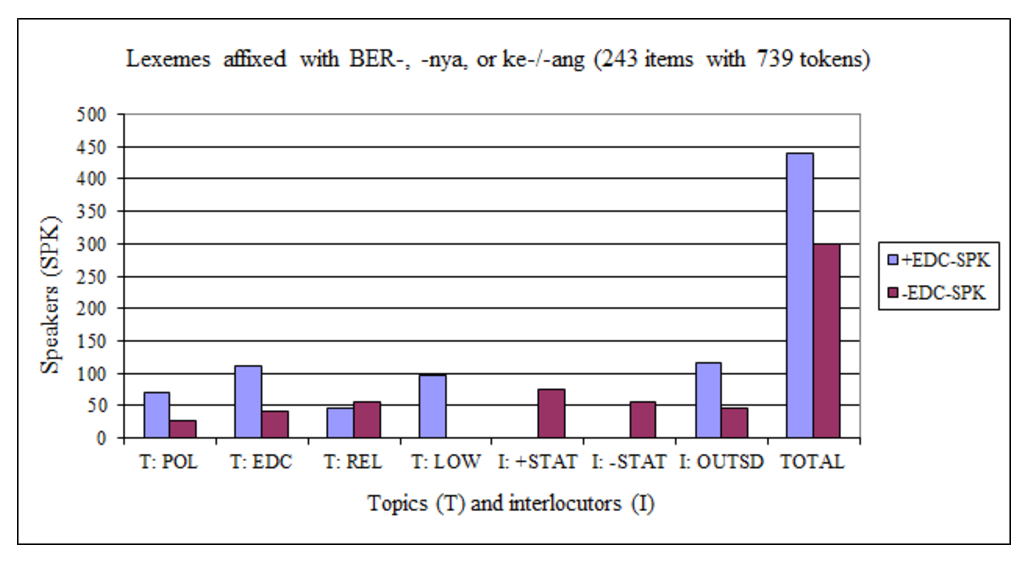
\includegraphics[scale=0.7]{./figures/Figure_3_4}
\resizebox{\textwidth}{!}{
\begin{tikzpicture}
  \begin{axis}[klugeaxis, y={}, height={.5\textheight}, width={\textwidth}, title={Lexemes affixed with \textscItal{ber}-, \textitbf{-nya}, or \textitbf{ke}\textitbf{-}/\textitbf{-}\textitbf{ang} (243 items with 739 tokens)}]
  \addplot[klugedots]	coordinates {(1,69)(2,112)(3,46)(4,97)(5,0)(6,0)(7,116)(8,440)};
  \addplot[klugelines] coordinates {(1,27)(2,40)(3,55)(4,0)(5,76)(6,55)(7,46)(8,299)};		
  \legend{\textsc{+edc-spk},\textsc{-edc-spk}}
  \end{axis}
  \end{tikzpicture}
  }
\caption[Token frequencies for lexemes affixed with {ber-}, \textitbf{-nya}, or \textitbf{ke}\textitbf{-}/\textitbf{-}\textitbf{ang} by speakers, topics, and interlocutors]{Token frequencies for lexemes affixed with \textscItal{ber-}, \textitbf{-nya}, or \textitbf{ke}\textitbf{-}/\textitbf{-}\textitbf{ang} by speakers, topics, and interlocutors}\label{Figure_3.4}
\end{figure}




The data presented in \tabref{Table_3.25} and \figref{Figure_3.4} shows that for the 243 affixed lexemes, most tokens (684/739 – 93\%) can be explained in terms of speaker education levels, topics, and/or role-relations between the speakers and their interlocutors (\textsc{ilct}).


Most tokens (440/739 – 60\%) were produced by \textsc{+edc-spk}, while 299/739 tokens (40\%) were produced by \textsc{-edc-spk}.

 
The \textsc{+edc-spk} produced about half of their tokens (227/440 – 52\%) when talking about \textsc{high} topics. Another 116/440 \textsc{+edc-spk} tokens (26\%) occurred during conversations with an outsider, namely the author (\textsc{outs}). The remaining 97/440 \textsc{+edc-spk} tokens (22\%) were produced during conversations with fellow-Papuans about \textsc{low} topics.



The \textsc{-edc-spk} produced 41\% of their tokens (122/299) while discussing \textsc{high} topics. Another 46/299 \textsc{-edc-spk} tokens (15\%) occurred during conversations with the author. The remaining \textsc{-edc-spk} tokens (131/299 – 44\%) were produced during conversations about \textsc{low} topics. Of these, 76/299 tokens (25\%) occurred when \textsc{-edc-spk} discussed \textsc{low} topics with \textsc{+stat} Papuans. The remaining 55/299 \mbox{\textsc{-edc-spk}} tokens (18\%) were produced during conversations with \textsc{-stat} Papuans, and 
therefore cannot be explained in terms of speaker education levels, topics, and/or role-relations. 
This total of 55 tokens refers to 7\% of the 739 tokens attested in the corpus.\footnote{As for the attested hapaxes, the findings of this domain analysis suggest that most are conditioned by the variables of speaker education levels, topics, and/or role-relations: 22/25 hapaxes prefixed with \textscItal{ber-}, 59/68 hapaxes suffixed with \textitbf{-nya}, and 18/22 hapaxes circumfixed with \textitbf{ke-}/\textitbf{-ang}. These items are best explained as code-switches with Indonesian. This leaves only three \textscItal{ber-}hapaxes, nine \textitbf{-nya}{}-hapaxes, and four \textitbf{ke-}/\textitbf{-ang}{}-hapaxes that are unaccounted for in terms of language external factors and that are likely to be the result of a productive \isi{word-formation} process. This, in turn, decreases the respective P values:
 
\begin{enumerate}[label=(\arabic*)]
\item for three \textscItal{ber-}hapaxes P=0.0183 (N=164) as opposed to P=0.0415 for 25 hapaxes (N=602) (N differs for the two P values, as six of the derived lexemes were excluded from the domain analysis),
\item for nine \textitbf{-nya}{}-hapaxes P=0.0284 (N=317) as opposed to P=0.1758 for 68 hapaxes (N=387) (N differs for the two P values, as one derived lexeme was excluded from the domain analysis), and
\item	 for four \textitbf{ke-}/\textitbf{-ang}{}-hapaxes P=0.0155 as opposed to P=0.0853 for 22 hapaxes (N=258).

\end{enumerate}
}

\section{Compounding}\label{Para_3.2}

Compounding denotes the “formation of a new lexeme by adjoining two or more lexemes” \citep[40]{Bauer.2003}. In Papuan Malay, however, the demarcation between compounds and phrasal expressions is unclear. That is, neither phonological, morphological, morphosyntactic, nor semantic criteria allow classifying word sequences unambiguously as either compounds or phrasal expressions, as shown in §\ref{Para_3.2.1}. The attested word combinations always have a binary structure in that they consist of two juxtaposed lexemes; the first component is always a \isi{noun}. More specifically, three types of word sequences can be distinguished, namely endocentric, exocentric, and coordinative ones, as discussed in §\ref{Para_3.2.2}. The main points on \isi{compounding} are summarized in §\ref{Para_3.3}.
 

\subsection{Demarcation of compounds from phrasal expressions}\label{Para_3.2.1}

Four different criteria have been suggested to distinguish compounds from phrasal expressions: phonological, morphological, morphosyntactic, and semantic criteria {\citep[24]{Aikhenvald.2007}}. They are discussed in turn in this section.



On phonological grounds, compounds can be distinguished from phrasal expressions in terms of their stress behavior. Compounds typically contain one primary stress, where\-as in phrasal expressions each phonological word carries its own stress {\citep[25]{Aikhenvald.2007}}. This criterion also applies to Papuan Malay, as shown in (\ref{Example_3.78}) and (\ref{Example_3.79}). In the \isi{compound} \textitbf{kacang-hijow} ‘mung bean’ in (\ref{Example_3.78}), the penultimate syllable carries primary stress, while secondary stress is assigned to the alternating syllable preceding the one carrying the primary stress. By contrast, in the \isi{phrasal expression} \textitbf{kacang hijow} ‘green bean’ in (\ref{Example_3.79}) each constituent carries its own stress. In fast speech, however, it is difficult to distinguish both constructions on phonological grounds. Instead, the context is the determining factor to establish the intended meaning.


% \todo{check example labelling}
\begin{styleExampleTitle}
{Phonological criteria}
\end{styleExampleTitle}
\ea
\label{Example_3.78}
\glll \textup{/ˌka.tʃaŋ.ˈhi.dʒɔw/} {} kacang-hijow\\ %
 { } { }  {bean-be.green}  \\
  { } { }  {‘mung bean’} \\
\z
\ea
\label{Example_3.79}
\glll \textup{/ˈka.tʃaŋ ˈhi.dʒɔw/} {}  kacang hijow\\ %
{} { }  {bean}  {be.green}  \\
{} { }  {‘green} {bean’} \\
\z


As for morphological criteria, compounds are typically distinct from phrasal expressions in that the former are marked with additional morphemes or have distinct constituent orders vis-à-vis phrasal expressions {\citep[26]{Aikhenvald.2007}}. In terms of morphological criteria, however, Papuan Malay compounds are not distinct from phrasal expressions. As illustrated in (\ref{Example_3.78}) and (\ref{Example_3.79}), neither construction has an additional morpheme that would mark it as a \isi{compound} or \isi{phrasal expression}. Neither are the two constructions distinct in terms of their constituent order, as in each case the head precedes the modifier.


On morphosyntactic grounds, compounds are usually distinct from phrasal expressions in that the components of a \isi{compound} cannot be separated by inserting other morphemes {\citep[26]{Aikhenvald.2007}}. Such an insertion leads to the loss of their \isi{compound} sense. This criterion also applies to Papuan Malay as shown in (\ref{Example_3.80}) and (\ref{Example_3.81}). When, for instance, the \isi{relativizer} \textitbf{yang} ‘\textsc{rel}’ is inserted in the \isi{compound} \textitbf{lemon-manis} ‘orange’ in (\ref{Example_3.80}), the \isi{compound} sense is lost. The result is the \isi{phrasal expression} \textitbf{lemon yang manis} ‘lemon which is sweet’ or ‘sweet lemon’ in (\ref{Example_3.81}).


 
\begin{styleExampleTitle}
{Morphosyntactic criteria}
\end{styleExampleTitle}
 
\ea
\label{Example_3.80}
\gll lemon-manis\\ %
lemon-be.sweet\\
 \glt ‘orange’\\
\z
 
\ea
\label{Example_3.81}
\gll lemon yang manis\\ %
{lemon} \textsc{rel} {be.sweet}\\
 \glt  ‘sweet lemon’ (Lit. ‘lemon which is sweet’)\\
\z



In cases such as the \isi{compound} \textitbf{orang-tua} ‘parent’ in (\ref{Example_3.82}) or the \isi{phrasal expression} \textitbf{orang tua} ‘old person’ in (\ref{Example_3.83}), however, it is difficult to distinguish both constructions on morphosyntactic grounds. Again, the context is the determining factor to establish the intended meaning.



\begin{styleExampleTitle}
{Ambiguities with respect to morphosyntactic criteria}
\end{styleExampleTitle} 
\ea
\label{Example_3.82}
\gll orang-tua\\ %
{person-be.old}\\
 \glt ‘parent’\\
\z 
\ea
\label{Example_3.83}
\gll orang tua\\ %
{person} {be.old}\\
 \glt ‘old person’\\
\z 


Semantically, compounds and phrasal expressions can be arranged on a scale from less to more compositional \citep[28]{Aikhenvald.2007}. The corpus, however, does not contain non-compositional compounds with idiosyncratic semantics.\footnote{While {\citet[28]{Aikhenvald.2007}} suggests that compounds can also be compositional, \citet[175]{Dryer.2007b} maintains that compounds have “an idiosyncratic meaning not predictable from the meaning of the component parts, as compared with syntactic compounds, in which one \isi{noun} is modifying a second \isi{noun} in a productive syntactic construction”.} This is illustrated in (\ref{Example_3.84}) to (\ref{Example_3.88}). Less compositional compounds are expressions such as \textitbf{kampung-tana} ‘home village’ in (\ref{Example_3.84}), or \textitbf{paduang-swara} ‘choir’ in (\ref{Example_3.85}). Compounds that are more compositional are those whose meaning is predictable from the meanings of its parts, such as \textitbf{air-mata} ‘tears’ in (\ref{Example_3.86}) or \textitbf{tali-prut} ‘intestines’ in (\ref{Example_3.87}). Very transparent compounds blend into phrasal expressions such as \textitbf{uang jajang} ‘pocket money’ or ‘money for snacks’ in (\ref{Example_3.88}). On the one hand one could say that \textitbf{uang jajang} ‘pocket money’ is a \isi{compound} with an idiosyncratic meaning. On the other hand one could argue that this construction has a phrasal structure that denotes a purpose relation between the nominal head \textitbf{uang} ‘money’ and its nominal modifier \textitbf{jajang} ‘snack’; hence, the construction \textitbf{uang jajang} ‘money for snacks’ is a \isi{phrasal expression} and not a \isi{compound}. Finally, there are phrasal expressions with clear compositional semantics, such as \textitbf{air sagu} ‘liquid of the sago palm tree’ in (\ref{Example_3.89}). (For details on \isi{noun} phrases with nominal modifiers see §\ref{Para_8.2.2}.)



\begin{styleExampleTitle}
{Semantic criteria}
\end{styleExampleTitle} 
\ea
\label{Example_3.84}
\gll kampung-tana\\ %
 village-ground\\
 \glt ‘home village’\\
\z  
\ea
\label{Example_3.85}
\gll paduang-swara\\ %
 fusion-voice\\
\glt 
‘choir’\\
\z 
\ea
\label{Example_3.86}
\gll air-mata\\ %
 water-eye\\ 
\glt  ‘tears’\\
\z 
\ea
\label{Example_3.87}
\gll tali-prut\\ %
 cord-stomach\\
\glt ‘intestines’\\
\z 
\ea
\label{Example_3.88}
\gll uang jajang\\ %
{money}  {snack}\\
\glt ‘pocket money’ / ‘money for snacks’\\
\z 
\ea
\label{Example_3.89}
\gll air  sagu\\ %
 {water} {sago} \\
\glt 
‘liquid of the sago palm tree’\\
\z

The data presented in this section shows that in Papuan Malay neither phonological, morphological, morphosyntactic, nor semantic criteria allow the unambiguous classification of word sequences as either compounds or phrasal expressions. Instead the data suggests that, following \citegen[14]{Lieber.2009} definition of \isi{compounding}, some Papuan Malay word combinations are “more compoundlike” while others are “less compoundlike [\ldots] with no clear categorical distinction” along this “cline”. The combinations range from less compositional two-word expressions such as \textitbf{kampung-tana} ‘home village’ to those with compositional transparent semantics such as \textitbf{air sagu} ‘liquid of the sago palm tree’. Given this lack of a clear demarcation between compounds and phrasal expressions, the term “\isi{collocation}” rather than “\isi{compound}” is used hereafter for such juxtaposed word sequences.\footnote{Collocations are defined as “word combinations which have developed an idiomatic semantic relation based on their frequent co-occurrence” (\citealt[200]{Bussmann.1996}; see also \citealt{Krishnamurthy.2006}).}


\subsection{Types of collocations}\label{Para_3.2.2}

In Papuan Malay, three types of collocations are found: endocentric, exocentric, and coordinative ones. In the following they are discussed one by one. 



In endocentric collocations, one component has head function while the subordinate component has modifying, content-specifying function, denoting “a sub-class of the items denoted by one of their elements” {\citep[42]{Bauer.2003}}. In Papuan Malay endocentric collocations, the head component always precedes the modifier component which can be a \isi{noun} or a stative \isi{verb}. Semantically, these ``\textsc{n} \textsc{n}'' or ``\textsc{n} \textsc{v}'' collocations encode different types of relationships between their components such as ``part-whole'', ``subtype-of'', or ``characteristic-of'' relations, as illustrated in \tabref{Table_3.26}. In addition, the corpus contains one \isi{collocation} in which the modifying component is a \isi{numeral}: \textitbf{segi-empat} ‘quadrangle’ (literally ‘side-four’).

\begin{table}
\caption{Endocentric ``\textsc{n} \textsc{n/v}'' collocations}\label{Table_3.26}

\begin{tabular}{llll}
\lsptoprule
 \multicolumn{1}{c}{Item} & \multicolumn{1}{c}{Gloss} & \multicolumn{1}{c}{Literal translation} &  \multicolumn{1}{c}{Semantic relation}\\
\midrule


\textitbf{tali-prut} & ‘intestines’ & ‘cord of the stomach’ & ‘Part-whole’\\

cord-stomach &  &  & \\
\\
\textitbf{lemon-manis} & ‘orange’ & ‘sweet lemon’ & ‘Subtype-of’\\

lemon-be.sweet &  &  & \\
\\
\textitbf{kreta-api} & ‘train’ & ‘carriage of fire’ & ‘Characteristic-of’\\

carriage-fire &  &  & \\

\lspbottomrule
\end{tabular}
\end{table}
% \todo[inline]{it is unclear to me how this should be modified}

In exocentric collocations, none of the constituents functions as its head. They “denote something which is not a sub-class” of either of their components; that is, “they are not hyponyms of either of their elements” {\citep[42]{Bauer.2003}}, as shown in \tabref{Table_3.27}. In the \isi{collocation} \textitbf{bapa-ade}, literally ‘father-younger.sibling’, for instance, neither of the two components serves as the content-specifying element. Likewise \textitbf{kepala-batu}, literally ‘head-stone’ does not refer to some kind of head. Instead, it denotes a ‘pig-headed person’. These examples also show that exocentric collocations typically consist of two juxtaposed nouns.

\begin{table}
\caption{Exocentric ``\textsc{n} \textsc{n}'' collocations}\label{Table_3.27}
\begin{tabular}{ll}
\lsptoprule
 \multicolumn{1}{c}{Item} & \multicolumn{1}{c}{Gloss}\\
\midrule

\textitbf{bapa-ade} & ‘father’s younger brother’(FyB) / ‘mother’s\\
father-ySb & younger sister’s husband’ (MyZH)\\
\tablevspace

\textitbf{kepala-batu} & ‘pig-headed person’\\
head-stone & \\
\tablevspace

\textitbf{mata-hari} & ‘sun’\\
eye-day & \\

\lspbottomrule
\end{tabular}
\end{table}


The distinction between endocentric and exocentric collocations is not always clear-cut, however, as shown in \tabref{Table_3.28}. The kinship terms \textitbf{bapa-tua} ‘uncle’ (literally ‘father-be.old’) and \textitbf{mama-tua} ‘aunt’ (literally ‘mother-be.old’) qualify as exocentric collocations on semantic grounds but as endocentric collocations on syntactic grounds. Both terms are exocentric in that they designate something which is not a sub-class of either of their components: \textitbf{bapa-tua} does not refer to an ‘old father’, neither does \textitbf{mama-tua} refer to an ‘old mother’. Instead, \textitbf{bapa-tua} denotes a ‘parent’s older brother’ (PoB) or a ‘parent’s older sister’s husband’ (PoZH), while \textitbf{mama-tua} designates a ‘parent’s older sister’ (PoZ) or a ‘parent’s older brother’s wife’ (PoBW). Syntactically, however, \textitbf{tua} ‘be old’ is subordinate to the head \textitbf{bapa}/\textitbf{mama} ‘father/mother’ and has modifying content-specifying function. Hence, both kinship terms also qualify as endocentric collocations.

\begin{table}
\caption{Endocentric versus exocentric collocations: Ambiguities}\label{Table_3.28}


\begin{tabular}{ll}
\lsptoprule
 \multicolumn{1}{c}{Item} &  \multicolumn{1}{c}{Gloss}\\
\midrule
\textitbf{bapa-tua} & ‘parent’s older brother’ (PeB) / ‘mother’s\\
father-be.old & ‘parent’s older sister’s husband’ (PeZH)\\
\tablevspace
\textitbf{mama-tua} & ‘parent’s older sister’ (PeZ) / ‘mother’s\\
mother-be.old & ‘parent’s older brother’s wife’ (PeBW)\\
\lspbottomrule
\end{tabular}
\end{table}

 

\begin{table}
\caption{Coordinative ‘\textsc{n} \textsc{n}’ collocations}\label{Table_3.29}


\begin{tabular}{lll}
\lsptoprule
 \multicolumn{1}{c}{Item} & \multicolumn{1}{c}{Gloss} &  \multicolumn{1}{c}{Semantic relation}\\
\midrule

\textitbf{ade-kaka} & siblings & Antonyms\\

ySb-oSb &  & \\
\\
\textitbf{kasi-sayang} & ‘deep love’ & Synonyms\\

love-love &  & \\
\\
\textitbf{guntur-kilat} & ‘thunderstorm’ & Different parts/aspects\\

thunder-lightning &  & \\
\\
\textitbf{tete-moyang} & ‘ancestors’ & Different parts/aspects\\

grandfather-ancestor &  & \\

\lspbottomrule
\end{tabular}
\end{table}

 Coordinative collocations designate entities made up of two nominal components that “can be interpreted as being joined by ‘and’” {\citep[351]{Bauer.2009}}. That is, in such collocations both components “are of semantically equal weight” {\citep[221]{Bussmann.1996}}. The nominal components can be antonyms, synonyms, or different parts or aspects of the designated concept, as shown in \tabref{Table_3.29}.

 
 \newpage 
\section{Summary}\label{Para_3.3}
\largerpage
This section briefly summarizes the main points on \isi{affixation} and \isi{compounding}.


\begin{enumerate}
\item 
Affixation


Affixation in Papuan Malay has very limited productivity. This conclusion is based on an investigation of six affixes: the prefixes \textscItal{ter-} ‘\textsc{acl}’, \textscItal{pe(n)-} ‘\textsc{ag}’, and \textscItal{ber-} ‘\textsc{vblz}’, the suffixes -\textitbf{ang} ‘\textsc{pat}’ and \textitbf{-nya} ‘\textsc{3possr}’, and the circumfix \textitbf{ke}-/-\textitbf{ang} ‘\textsc{nmlz}’. Given the \isi{sociolinguistic profile} of Papuan Malay (substantial language contact between Papuan Malay and Indonesian with both languages being in a diglossic distribution, positive to somewhat am\isi{bivalent} language attitudes toward Papuan Malay, and lack of language awareness of many Papuan Malay speakers) no productivity testing was conducted, as a substantial amount of interference from Indonesian was expected. This interference would have skewed testees’ naïve judgments. Instead, the six affixes were examined in terms of six language internal and three language external factors considered relevant in establishing the degree of productivity of these affixes.



The results of this investigation are as follows:
\begin{enumerate}

\item 
Papuan Malay \textscItal{ter-} ‘\textsc{acl}’ has limited productivity; it indicates accidental or unintentional actions or events. In other \ili{eastern Malay varieties} and in Standard Malay, the prefix is rather productive; here it likewise signals accidental or unintentional actions or events.
\item 
Papuan Malay -\textitbf{ang} ‘\textsc{pat}’ has limited productivity; it typically designates the patient or result of an action, event or state. As for other \ili{eastern Malay varieties}, the suffix is only mentioned for \ili{Ambon Malay}; its degree of productivity is unclear. In Standard Malay the suffix is very productive. Both in Ambon and in Standard Malay, the suffix also indicates the patient or product of an action, event or state.
\item 
Papuan Malay \textscItal{pe(n)-} ‘\textsc{ag}’ has marginal productivity, at best. It typically denotes the subject of the action, event, or state specified by the \isi{verbal base}; some of the affixed lexemes also receive an intensified intransitive or monotransitive reading. As for other \ili{eastern Malay varieties}, the prefix seems to have retained its productivity only in \ili{Ternate Malay}. In Standard Malay, the suffix is very productive. In other Malay varieties the prefix likewise denotes the subject of the action, event, or state specified by the \isi{verbal base}. A verbal interpretation, but not the intensified reading, is also reported for other \ili{eastern Malay varieties}. In Standard Malay, by contrast, only derivations with \isi{monovalent} stative bases can function as \isi{monovalent} stative verbs.
\item 
In Papuan Malay, prefix \textscItal{ber-} ‘\textsc{vblz}’ is unproductive, whereas in other \ili{eastern Malay varieties} and Standard Malay the prefix is very productive.
\item 
In Papuan Malay, \textitbf{-nya} ‘\textsc{3possr}’ and \textitbf{ke}\textitbf{-}/\textitbf{-}\textitbf{ang} ‘\textsc{nmlz}’ are unproductive. The same applies to other \ili{eastern Malay varieties}, while both affixes are very productive in Standard Malay.
\end{enumerate}

\item 
Compounding


In Papuan Malay, the demarcation between compounds and phrasal expressions is unclear. Neither phonological, morphological, morphosyntactic, nor semantic criteria allow the unambiguous classification of two juxtaposed nouns as compounds or phrasal expressions. Therefore, the term “\isi{collocation}” is employed as a cover term for such word combinations that differ in transparency from non-com\-posi\-tional idiosyncratic semantics to compositional transparent semantics. Three different types of collocations are attested, endocentric, exocentric, and coordinative ones. Given the lack of a clear demarcation between compounds and phrasal expressions, it remains unclear to what degree \isi{compounding} is a productive process.
\end{enumerate}


% % copy the lines above and adapt as necessary

%%%%%%%%%%%%%%%%%%%%%%%%%%%%%%%%%%%%%%%%%%%%%%%%%%%%
%%%                                              %%%
%%%             Backmatter                       %%%
%%%                                              %%%
%%%%%%%%%%%%%%%%%%%%%%%%%%%%%%%%%%%%%%%%%%%%%%%%%%%%

% There is normally no need to change the backmatter section
\backmatter
\phantomsection%this allows hyperlink in ToC to work
\printbibliography[heading=references] 
\cleardoublepage

\phantomsection 
\addcontentsline{toc}{chapter}{Index} 
\addcontentsline{toc}{section}{Name index}
\ohead{Name index} 
\printindex 
\cleardoublepage
  
\phantomsection 
\addcontentsline{toc}{section}{Language index}
\ohead{Language index} 
\printindex[lan] 
\cleardoublepage
  
\phantomsection 
\addcontentsline{toc}{section}{Subject index}
\ohead{Subject index} 
\printindex[sbj]
\ohead{} 

\cleardoublepage

\includepdf[pages=1]{./LSP/lsp-graphics/didyoulikethisbook}
\end{document} 

% you can create your book by running
% xelatex main.tex
%
% you can also try a simple 
% make
% on the commandline
